\documentclass[11pt,          % font size: 11pt or 12pt
               phd,           % degree:    ms or phd
               onehalfspacing % spacing: onehalfspacing or doublespacing
               ]{ncsuthesis}

%%----------------------------------------------------------------------------%%
%%------------------------------ Import Packages -----------------------------%%
%%----------------------------------------------------------------------------%%

\usepackage{booktabs}  % professionally typeset tables
\usepackage{amsmath}%,amssymb,amsfonts}
\usepackage{textcomp}  % better copyright sign, among other things
%\usepackage{xcolor}
\usepackage{lipsum}    % filler text
%\usepackage{subfig}    % composite figures

%%ORTIZ PACKAGES

%%----------------------------------------------------------------------------%%
%%--------------------------- Personal Packages ------------------------------%%
%%----------------------------------------------------------------------------%%

%\usepackage{comment}
%\usepackage{algorithm,algorithmic}
\usepackage{algorithmic}
\usepackage[ruled, vlined, linesnumbered]{algorithm2e}
\usepackage{tabularx}
\usepackage{multirow}
\usepackage[list=true,justification=centering]{subcaption}
%\usepackage[format=plain,justification=RaggedRight,singlelinecheck=true,font=large,labelfont=bf,labelsep=space]{caption}
\usepackage[format=plain,justification=justified,singlelinecheck=true,font=large,labelfont=bf,labelsep=space]{caption} 
\usepackage{adjustbox}
\usepackage{mfirstuc}
\usepackage{xspace}
\usepackage{enumitem,kantlipsum}
\usepackage{grffile}
\usepackage{pbox}
\usepackage{pifont}% http://ctan.org/pkg/pifont
\newcommand{\cmark}{\ding{51}}%
\newcommand{\xmark}{\ding{55}}%
\newcommand{\what}{{\bf WHAT }}
% for upside down traingle
\newcommand{\custriangle}{\includegraphics[scale=0.5]{Figures/upsidedown.png}}
\newcommand{\cuscross}{\includegraphics[scale=0.4]{Figures/cross.png}}
\newcommand{\cusdot}{\includegraphics[scale=0.5]{Figures/dot.png}}


%%%%%%%%%%%%%%%%%%%%%%%%%%%%%%%%%%%%%%%%%%
%%%%%%%%%%% Old bibliography commands
%%%%%%%%%%%%%%%%%%%%%%%%%%%%%%%%%%%%%%%%%%5
%\usepackage[super,sort&compress,comma,square,authoryear]{natbib} %\cite command %Added by Ortiz

%use the following line with plainnat
%\usepackage[super,sort&compress,comma,square,numbers]{natbib} %\cite command %Added by Ortiz
%\usepackage{natbib}

%\usepackage[style=alphabetic,natbib=true,backend=bibtex
%sorting=nyt,firstinits=true,isbn=false,doi=false,url=false]{biblatex} %couldn't get backend=biber to work

%\usepackage{filecontents}

%\bibliography{Ortiz-thesis2}
%\bibliographystyle{plain}


%%%%%%%%%%%%%%%%%%%%%%%%%%%%%%%%%%%%%%%%%%
%%%%%%%%%%% Hack for alphanumeric bibliography
%%%%%%%%%%%%%%%%%%%%%%%%%%%%%%%%%%%%%%%%%%5
\RequirePackage[
			style=numeric-comp,%alphabetic,%numeric-comp,%authoryear-comp,%
			sorting=nyt,%ynt					
			hyperref=true, %	
			firstinits=true,%
			backend=bibtex,
			natbib=true,
			url=false,
			isbn=false,
			maxnames=2, %for et al to be used
			maxalphanames=1, %to avoid printing a + for every et al in the abbreviation
			doi=false]{biblatex}		
			

%needed to do et al after two names
%http://tex.stackexchange.com/questions/44048/use-et-al-in-biblatex-custom-style
\renewcommand*{\finalnamedelim}{\addspace\&\space}

%Simplify abbreviation (the default uses either one or two authors and it indicates et al with a +)
%The following five lines make it so that only the first author is used in the abbreviation
%http://tex.stackexchange.com/questions/27956/label-only-from-first-author
\renewcommand*{\labelalphaothers}{}
    \renewcommand*{\intitlepunct}{}
    \DefineBibliographyStrings{german}{in={}}
    \DefineBibliographyStrings{english}{in={}}
    \DeclareNameAlias{sortname}{last-first}
    \DeclareNameAlias{default}{last-first}
	
%\AtEveryCitekey{\ifciteseen{}{\defcounter{maxnames}{99}}} %authoryear			
\DeclareFieldFormat[article,periodical]{volume}{\mkbibbold{#1}}
\makeatletter

\newrobustcmd*{\parentexttrack}[1]{%
  \begingroup
  \blx@blxinit
  \blx@setsfcodes
  \blx@bibopenparen#1\blx@bibcloseparen
  \endgroup}

\AtEveryCite{%
  \let\parentext=\parentexttrack%
  \let\bibopenparen=\bibopenbracket%
  \let\bibcloseparen=\bibclosebracket}

\makeatother
\renewcommand{\cite}[1]{\parencite{#1}}


\renewbibmacro{in:}{%
  \ifentrytype{article}{}{%
  \printtext{\bibstring{in}\intitlepunct}}}
  
\AtEveryBibitem{\clearfield{month}}

\AtEveryBibitem{\clearfield{language}}
%%%%%%%%%%%%%%%%%%%%%%%%%%%%%%%%%%%%%%%%%%%%%

%\addbibresource{Ortiz-thesis2.bib}
%\addbibresource{Ortiz-thesisURL.bib}
\addbibresource{thesis.bib}
\addbibresource{conference.bib}

 \defbibheading{myheading}[REFERENCES]{
 \chapter*{#1}
 %\centerline{\bf{#1}}
 \markboth{#1}{#1}}

%\usepackage{amsmath,amssymb,amsfonts} %amssymb and amsfonts cannot be used in conjunction with mdput
%\usepackage{graphicx,subfig}% Include figure files
\usepackage{dcolumn}% Align table columns on decimal point
\usepackage{bm}% bold math
%\usepackage{hyperref}% add hypertext capabilities
%\usepackage{hypernat}% make hyperref and natbib work together
\usepackage{cancel}
\usepackage{verbatim}% multiline commenting
\usepackage{ifthen}
\usepackage{url}
\urlstyle{same}
\usepackage{sectsty}
\usepackage{balance} 
%\usepackage{caption}
\usepackage{graphicx} %eps figures can be used instead
\usepackage{lastpage}
\usepackage{fancyhdr}
\pagestyle{fancy}

%http://tex.stackexchange.com/questions/100817/error-when-using-bc-from-abbrevs-in-caption
%Getting BC
\usepackage{abbrevs}
\usepackage{etoolbox}
\robustify{\DateMark} % after having loaded abbrevs

\usepackage{units} %Needed to solve bug from citation Hydrodynamics in 21/2 dimensions
%see http://www.latex-community.org/viewtopic.php?f=5&t=989

\usepackage[sharp]{easylist} %used for brainstorming purposes 
%\usepackage{mathabx} % used for \Asterisk for convolution %conflicts with \widering

%compile on single pass
%\usepackage[backend=biber,...]{biblatex}


%%%%%%%%%%%%
%%% Hack to make chapters start on odd pages
% http://tex.stackexchange.com/questions/73591/how-to-have-a-blank-even-page-before-every-chapter
%%%%%%%%%%%%
%\newcommand{\ensureoddstart}{\checkoddpage\ifoddpage\else\newpage\mbox{}\fi}
%\newcommand{\ensureoddstart}{}


%%%Fancy tables
%http://tex.stackexchange.com/questions/94032/fancy-tables-in-latex
\usepackage[table]{xcolor}
\usepackage{array,booktabs}
\usepackage{colortbl}
\newcolumntype{L}{@{}>{\kern\tabcolsep}l<{\kern\tabcolsep}}



%%%%%%%%%%
%%%%% Hack to allow more levels in outline
%%%%%%%%%%
%\setcounter{secnumdepth}{5}
%\setcounter{tocdepth}{5} %may violate ETD
%Usage http://pleasemakeanote.blogspot.com/2010/06/how-to-activate-subsubsubsection-in.html
%\section{} % level 1
%\subsection{} % level 2
%\subsubsection{} % level 3
%\paragraph{} % level 4 - equivalent to subsubsubsection
%\subparagraph{} % level 5

%http://tex.stackexchange.com/questions/60209/how-to-add-an-extra-level-of-sections-with-headings-below-subsubsection
\usepackage{titlesec}

\setcounter{secnumdepth}{4}

\titleformat{\paragraph}
{\normalfont\normalsize\bfseries}{\theparagraph}{1em}{}
\titlespacing*{\paragraph}
{0pt}{3.25ex plus 1ex minus .2ex}{1.5ex plus .2ex}

\usepackage{listings}
\definecolor{MyDarkBlue}{rgb}{0,0.08,0.45} 
\lstset{
    language=Python,
    basicstyle=\ttfamily\fontsize{2.7mm}{0.8em}\selectfont,
    breaklines=true,
    prebreak=\raisebox{0ex}[0ex][0ex]{\ensuremath{\hookleftarrow}},
    frame=l,
    showtabs=false,
    showspaces=false,
    showstringspaces=false,
    keywordstyle=\bfseries,
    emph={furthest,gale,better,improved,where,fastmap,split,project,mutate,mutate1}, emphstyle=\bfseries\color{blue},
    stringstyle=\color{green!50!black},
    commentstyle=\color{gray}\itshape,
    numbers=left,
    captionpos=t,
    escapeinside={\%*}{*)}
}
\usepackage{commath}
\usepackage{mathtools}
\newcommand{\bi}{\begin{itemize}}%[leftmargin=0.4cm]}
\newcommand{\ei}{\end{itemize}}
\newcommand{\be}{\begin{enumerate}}
\newcommand{\ee}{\end{enumerate}}
\newcommand{\tion}[1]{\S\ref{sect:#1}}
\newcommand{\fig}[1]{Figure~\ref{fig:#1}}

\newcommand{\tab}[1]{Table ~\ref{tab:#1}}
\newcommand{\eq}[1]{Equation~\ref{eq:#1}}

\usepackage{xcolor}
\definecolor{whatcolor}{HTML}{d9d9d9}
\definecolor{guocolor}{HTML}{999999}

\usepackage{xcolor,soul}
\definecolor{LightGray}{gray}{0.975}
\definecolor{Mygreen}{HTML}{228B22}
\definecolor{Myred}{HTML}{800000}
\DeclareRobustCommand{\hlgreen}[1]{{\sethlcolor{Mygreen}\textcolor{white}{\hl{#1}}}}
\DeclareRobustCommand{\hlyellow}[1]{{\sethlcolor{yellow}\hl{#1}}}
\DeclareRobustCommand{\hlred}[1]{{\sethlcolor{Myred}\textbf{\textcolor{white}{\hl{#1}}}}}
\newcommand{\flash}{{\sc Flash}\xspace}

%%% graph
\newcommand{\crule}[3][darkgray]{\textcolor{#1}{\rule{#2}{#3}}}
%\newcommand{\rone}{\crule{1mm}{1.95mm}}
%\newcommand{\rtwo}{\crule{1mm}{1.95mm}\hspace{0.3pt}\crule{1mm}{1.95mm}}
%\newcommand{\rthree}{\crule{1mm}{1.95mm}\hspace{0.3pt}\crule{1mm}{1.95mm}\hspace{0.3pt}\crule{1mm}{1.95mm}}
%\newcommand{\rfour}{\crule{1mm}{1.95mm}\hspace{0.3pt}\crule{1mm}{1.95mm}\hspace{0.3pt}\crule{1mm}{1.95mm}\hspace{0.3pt}\crule{1mm}{1.95mm}} 
%\newcommand{\rfive}{\crule{1mm}{1.95mm}\hspace{0.3pt}\crule{1mm}{1.95mm}\hspace{0.3pt}\crule{1mm}{1.95mm}\hspace{0.3pt}\crule{1mm}{1.95mm}}
\newcommand{\quart}[3]{\begin{picture}(100,6)%1
{\color{black}\put(#3,3){\circle*{4}}\put(#1,3){\line(1,0){#2}}}\end{picture}}
\newcommand{\quartex}[3]{
\begin{picture}(25,6)%1
    {
        \color{black}
        \put(#3,3)
        {\circle*{4}}
        \put(#1,3)
        {\line(1,0){#2}}
    }
\end{picture}
}

%%%%%%%%%%%%%%%%%%%%%%%%%%
%%%% Hack for containing figures within sections
%%%%%%%%%%%%%%%%%%%%%%%%%%%%
%http://ctan.org/pkg/placeins
\usepackage{placeins}
%De?ج�?�fines a \FloatBar?ج�?�rier com?ج�?�mand, be?ج�?�yond which floats may not pass; use?ج�?�ful, for ex?ج�?�am?ج�?�ple, to en?ج�?�sure all floats for a sec?ج�?�tion ap?ج�?�pear be?ج�?�fore the next \sec?ج�?�tion com?ج�?�mand.

%%%Hack for centering all figures
%\makeatletter
%\g@addto@macro\@floatboxreset\centering
%\makeatother

%%----------------------------------------------------------------------------%%
%%---------------------------- Formatting Options ----------------------------%%
%%----------------------------------------------------------------------------%%
%%

%% -------------------------------------------------------------------------- %%
%% Disposition format -- any titles, headings, section titles
%%  These formatting commands affect all headings, titles, headings,
%%  so sizing commands should not be used here.
%%  Formatting options to consider are
%%     +  \sffamily - sans serif fonts.  Dispositions are often typeset in
%%                    sans serif, so this is a good option. 
%%     +  \rmfamily - serif fonts
%%     +  \bfseries - bold face
%\dispositionformat{\sffamily\bfseries}   % bold and sans serif
\dispositionformat{\bfseries}            % bold and serif

%% -------------------------------------------------------------------------- %%
%% Formatting for centered headings - Abstract, Dedication, etc. headings
%%  This is where one might put a sizing command.
%%  \MakeUppercase can be used to typeset all headings in uppercase.
\headingformat{\large\MakeUppercase}   % All letters uppercase
%\headingformat{\large}                % Not all uppercase
%\headingformat{\Large\scshape}        % Small Caps, used with serif fonts.

%% Typographers recommend using a normal inter-word space after
%% sentences. TeX's default is to add an wider space, but \frenchspacing
%% gives a normal spacing. Comment out the following line if you prefer
%% wider spaces between sentences.
\frenchspacing


%% -------------------------------------------------------------------------- %%
%%  Optional packages
%%    A number of compatible packages to improve the look and feel of
%%    your document are available in the file optional.tex 
%%    (For example, hyperlinks, fancy chapter headings, and fonts)
%% To use these options, uncomment the next line and see optional.tex
\include{optional}
%solve bug from fancyhdr in optional
%http://nw360.blogspot.com/2006/11/latex-headheight-is-too-small.html
\setlength{\headheight}{14pt}

%%----------------------------------------------------------------------------%%
%%---------------------------- Content Options -------------------------------%%
%%----------------------------------------------------------------------------%%
%% Size of committee: 3, 4, 5, or 6 -- this number includes the chair
\committeesize{4}

%% Members of committee
%%  Each of the following member commands takes an optional argument
%%   to specify their role on the committee.
%%  For co-chairs, use the commands:
%%      \cochairI{Doug Dodd}
%%      \cochairII{Chris Cox}
%%
\chair{Dr. Timothy J. Menzies}
\memberI{Dr. Kathyrn Stolee}
\memberII{Dr. Min Chi}
\memberIII{Dr. Ranga Raju Vatsavai, Ph.D. }   % unnecessary if committeesize=3
%\memberIV{Hung-Wei Tseng}    % unnecessary if committeesize=3 or 4
%\memberV{Edna Everitt}  % unnecessary if committeesize=3, 4, or 5


%% Student writing thesis, \student{First Middle}{Last}
\student{Vivek}{Nair} % a full middle name
%\student{John M.}{Smith} % a middle initial

%% Degree program
\program{Computer Science}

%% Thesis Title
%%  Keep in mind, according to ETD guidelines:
%%    +  Capitalize first letter of important words.
%%    +  Use inverted pyramid shape if title spans more than one line.
%%
%%  Note: To break the title onto multiple lines, use \break instead of \\.
%\thesistitle{A North Carolina State University Sample \LaTeX{} Thesis \break 
%with a Title So Long it Needs a Line Break}
% TODO: add verb, right now only with subject
%\thesistitle{Elastic Data-Intensive Computing for the Cloud}
\thesistitle{Frugal ways to find Good Configurations}

%% Degree year.  Necessary if your degree year doesn't equal the current year.
%\degreeyear{1995}


%%----------------------------------------------------------------------------%%
%%---------------------------- Personal Macros -------------------------------%%
%%----------------------------------------------------------------------------%%

%% A central location to add your favorite macros.

%% A few examples to get you started.
\newcommand{\uv}[1]{\ensuremath{\mathbf{\hat{#1}}}}
%\newcommand{\bo}{\ensuremath{\mathbf{\Omega}}}
\newcommand{\eref}[1]{Eq.~\ref{#1}}
\newcommand{\fref}[1]{Fig.~\ref{#1}}
\newcommand{\tref}[1]{Table~\ref{#1}}
%\newcommand{\del}{\nabla}
\renewcommand{\exp}[1]{e^{#1}}
\newcommand{\Conv}{\mathop{\scalebox{1.5}{\raisebox{-0.2ex}{$\ast$}}}}%



\usepackage{color}
%\newcommand{\NEW}[1]{\textcolor{blue}{#1}}
\newcommand{\NEW}[1]{#1}
%% conflict with the algorithmc package?
%\newcommand{\COMMENT}[1]{\textcolor{green}{#1}}


\newcommand{\NOTER}[1]{\textcolor{orange}{#1}}
\newcommand{\NOTEC}[1]{\textcolor{blue}{#1}}
\newcommand{\NOTEK}[1]{\textcolor{magenta}{#1}}

\newcommand{\mum}{\ensuremath{{\mu}\text{m}}}


\setlength{\fboxsep}{0pt}
\usepackage[framemethod=tikz]{mdframed}
\usepackage{lipsum}
\usetikzlibrary{shadows}
\newmdenv[
tikzsetting= {fill=white!20},
linewidth=2pt,
roundcorner=5pt, 
shadow=true
]{myshadowbox}



% words
%\newcommand{\fig}[1]{Fig. #1}
\newcommand{\myfigure}[1]{Figure~#1}
\newcommand{\mytable}[1]{Table~#1}
\newcommand{\naive}{na\"ive\xspace}
\newcommand{\etal}{\textit{et al}.\xspace}
\newcommand{\ie}{\textit{i}.\textit{e}.,\xspace}
\newcommand{\eg}{\textit{e}.\textit{g}.,\xspace}
\newcommand{\etc}{\textit{etc}.\xspace}
%\newcommand{\rone}[1]{{\color{black} #1}}
%\newcommand{\rtwo}[1]{{\color{black} #1}}
\newcommand{\todo}[1]{\textbf{{\color{blue} #1}}}
\newcommand{\quotes}[1]{``#1''}
\newcommand{\myequation}[1]{Equation~#1}


%This makes it so that you can add short paths in your .tex by including the folders where you store your images in the search path
\graphicspath{
{./Chapter-Introduction/}
{./Chapter-Introduction/figures}
{./Chapter-Background/}
{./Chapter-Background/figures/}
{./Chapter-WHAT/}
{./Chapter-WHAT/figures/}
{./Chapter-Rank/}
{./Chapter-Rank/figures/}
{./Chapter-Flash/}
{./Chapter-Flash/figures/}
{./Chapter-Conclusion/}
{./Chapter-Conclusion/figures/}
}

%%---------------------------------------------------------------------------%%
\usepackage{calc}
%% Capital letter height
\newlength{\chaptercapitalheight}
\settoheight{\chaptercapitalheight}{D}
\newlength{\chapterfootskip}
\setlength{\chapterfootskip}{\chaptercapitalheight}
\addtolength{\chapterfootskip}{2\baselineskip}
\addtolength{\chapterfootskip}{0.5ex}  % A little extra space to ensure there are 2 full double spaced lines
%\def\chapterfootskipnum{\chapterfootskip}
\renewcommand{\listfigurename}{LIST OF FIGURES}
\renewcommand{\listtablename}{LIST OF TABLES}
\renewcommand{\bibname}{BIBLIOGRAPHY}

%\renewcommand{\cfttoctitlefont}{\centering\ncsu@headingformat}


%http://tex.stackexchange.com/questions/47184/height-of-figure-caption-textheight
\newlength\graphht
\newcommand\calculategraphicstargetheight[1]{%
     \setlength\graphht{\textheight 
                       -\parskip
                       -\abovecaptionskip -\belowcaptionskip
                       -(12pt * #1) % assuming baselineskip of 12pt in caption
                       -\chapterfootskip
                       }}

%\usepackage{titlesec}

%landscape support in fancyhdr from http://tex.stackexchange.com/questions/9071/how-to-translate-and-rotate-the-heading-of-landscaped-pages
\usepackage{pdflscape}
\usepackage{tikz}
\fancypagestyle{lscapedplain}{%
  \fancyhf{}
  \fancyfoot{%
    \tikz[remember picture,overlay]
      \node[outer sep=1cm,above,rotate=90] at (current page.east) {\thepage};}
\renewcommand{\headrulewidth}{0pt} 
\renewcommand{\footrulewidth}{0pt}
}

%\includeonly{front}
%\includeonly{Chapter-1/main}
                      
\begin{document}
\pagestyle{plain}
%%---------------------------------------------------------------------------%%
\frontmatter

%% ------------------------------ Abstract ---------------------------------- %%
\begin{abstract}
Most software systems available today are configurable, which gives the users an option to customize the system to achieve differ-
ent functional or non-functional (better performance) properties. As systems evolve, more configuration options are added to the
software system. Studies report that developers find it difficult to
understand the configuration spaces, which leaves considerable
optimization potential untapped and induces major economic cost.
To solve this problem of finding the (near) optimal configurations,
engineers have proposed various techniques. Most popular among
them are model-based techniques, where accurate models of the configuration space are created using as few configuration measurements as possible. We notice two major problems with the model-based techniques: 1) previous techniques are expensive to be practically viable, and 2) there are software systems whose configuration spaces cannot be accurately modeled. Consequently, there is
a gap between proposed techniques and practical viability of these
techniques.
This dissertation will focus on proposing techniques which are
easier to understand and is practically viable. 

First, we present \textbf{WHAT} that exploits
some lower dimensional knowledge to build performance models. Prior work on
predicting the performance of software configurations suffered from either (a) requiring
far too many sample configurations or (b) large variances in their predictions.
Both these problems can be avoided using the \textbf{WHAT} spectral learner. WHAT\textquotesingle s innovation
is the use of the spectrum (eigenvalues) of the distance matrix between the
configurations of a configurable software system, to perform dimensionality reduction.
Within that reduced configuration space, many closely associated configurations
can be studied by executing only a few sample configurations. For the subject systems
studied here, a few dozen samples yield accurate and stable predictors?less than
10 \% prediction error, with a standard deviation of less than 2\%. When compared
to the state of the art, WHAT (a) requires 2 to 10 times fewer samples to achieve
similar prediction accuracies, and (b) its predictions are more stable (i.e., have lower
standard deviation). Furthermore, we demonstrate that predictive models generated
by WHAT can be used by optimizers to discover system configurations that closely
approach the optimal performance.


The second contribution is a rank-based method
which shows how an accurate model is not required for performance optimization, but a rank-preserving model is sufficient. We evaluate rank-based method with 21 scenarios based on nine software systems and demonstrate that our approach is beneficial in 16 scenarios; for the remaining five scenarios, an accurate model
can be built by using very few samples anyway, without the need
for a rank-based approach. Additionally, in 8/21 of the scenarios,
the number of measurements required by the rank-based method
is an order of magnitude smaller than methods used in prior work.
To further improve our second contribution, we also propose a
Bayesian-based method called Flash: an alternative to model-based
technique. Based on preliminary evidence, which can further reduce
the cost of performance optimization. 


Finally, we present \textbf{FLASH},  a sequential model-based method, which sequentially explores the configuration space by reflecting on the configurations evaluated so far to determine the next best configuration to explore. FLASH scales up to software systems that defeat the prior state of the art model-based methods in this area. FLASH runs much faster than existing methods and can solve both single-objective and multi-objective optimization problems. The central insight of this paper is to use the prior knowledge (gained from prior runs) to choose the next promising configuration. This strategy reduces the effort (ie, number of measurements) required to find the (near) optimal configuration. We evaluate FLASH using 30 scenarios based on 7 software systems to demonstrate that FLASH saves effort in 100\% and 80\% of cases in single-objective and multi-objective problems respectively by up to several orders of magnitude compared to the state of the art techniques.

\end{abstract}


%% ---------------------------- Copyright page ------------------------------ %%
%% Comment the next line if you don't want the copyright page included.
\makecopyrightpage

%% -------------------------------- Title page ------------------------------ %%
\maketitlepage

%% -------------------------------- Dedication ------------------------------ %%
\begin{dedication}
%\centering{
\begin{center}
To Ammayi---for timely advice and support
\end{center}

\end{dedication}

%% -------------------------------- Biography ------------------------------- %%
\begin{biography}
Vivek Nair was born and raised in the city of Kolkata, India. He graduate from West Bengal University of Technology and National Institute of Technology, Durgapur with and Bachelors in Technology and Master in Technology respectively. 
 His primary research interest is search based software engineering with a primary goal to solve search problems to maximize the quality of the search while minimizing the cost of search.  His current research investigated problems in the software engineering domain and developed techniques not only to solve software configuration problem, but also software product lines as well as cloud architecture tuning problems.  Before joining the PhD program, he
had two years of professional experience in the Samsung Software Engineering Labs. 
During his PhD program, his internship experiences include Lexisnexis Risk Solutions (2015-2017), and
Microsoft Research - Redmond, USA (Summer 2018). He is a student member of IEEE.


\end{biography}

%% ----------------------------- Acknowledgements --------------------------- %%
\begin{acknowledgements}
\textit{*This acknowledgment contains plenty of subtexts and would be found as text within brackets. The subtext is meant to serve the purpose of comic relief and comic relief only.} \\

This thesis is no way an individual work. It is a product of a lot of love and sacrifice, tears and sweat of not just me but for various individuals who have taught lessons throughout my journey as a graduate student, here at NCSU. Although, I have endeavored to acknowledge everyone who has touched my life [for better or for worse], this list is in no way comprehensive. 

One of the primary reasons, I can write this thesis is because of Dr. George N. Rouskas and my aunt, Dr. Latha Unni. 
My first year at NCSU was tumultuous and eventful. As new graduate student, dealing with the stresses of graduate school and the unfavorable environment of my previous lab was overwhelming. This resulted in me [prematurely] deciding to quit graduate school---which I have been so excited to attend. Dr. Rouskas, who provided me with financial support while transitioning from my old advisor to my current advisor. Dr. Rouskas and my aunt counseled and provided support when I needed it the most. This thesis would have never been possible without these two amazing people. 

Secondly my thesis advisor [my academic father], Dr. Menzies, he is a legend [faking the
Aussie accent]. He has been very [not so] patient with me and directed me towards areas which
held promise. He helped me understand the value of collaboration and being a voracious reader
of the literature. That said I have never had a more dramatic relationship with anyone, which
in retrospect is an effective way of training graduate student. Our story has all the elements
of a soap opera, there are love and respect, not so much love [hate sounds just too strong] and
doubt. Either way, he played a massive part in making this thesis possible and made me a better
researcher [hopefully]. Also, he is also a reason I went to a trip around Europe [with Dr. Fu and George].

Thirdly, I would then like to thank my dissertation committee members,
Dr. Ranga Raju Vatsavai, Dr. Min Chi and Dr. Kathryn T. Stolee,
for their valuable feedback and insight on my dissertation.

I am also grateful to my research collaborators: Sven Apel (University of Passau), Norbert Siegmund (Bauhaus-University Weimar), and Pooyan Jamshidi (University of South Carolina), Jianfeng Chen (North Carolina State University).  I would like to gratefully acknowledge researchers who generously shared their research tools and results used in my dissertation.  I am very much
thankful to all my peers at the RAISE Lab, for their constant support, and useful feedback on
my research. I thank Dr. Wei Fu, Dr. Chin-Jung Hsu, Rahul Krishna, George Mathew, and Zhe Yu for the insightful and exciting conversations [interestingly I was able to write papers with all these amazing individuals---so all our discussions were not completely useless---as noted by Dr. Fu in his thesis acknowledgement]. 
I thank my internship mentors in the industry, who have immensely helped me expand
my research to a broader scope: Dan Camper and Arjuna Chala (LexisNexis Risk Solutions), and Chris Duvarney, Kim Herzig, and Hitesh Sajnani (Microsoft Research, USA). 


I extend heartfelt thanks to Kathy Luca, Carol Allen, and all the helpful staff at the Department
of Computer Science. I thank Amruthkiran Hedge, Anand Gorthi, Sandesh Saokar, Siddartha Chauhan, Mayank Vaish, Akhilesh Tanneru [Mr. T], and George Mathew for
sharing the apartment and making my stay at Raleigh eventful. Special thanks to Karen Warmbein, Blue and [Z]Simba whose love and support helped me survive the grind.



Finally, last but not least, I am very thankful to my family and friends. My family and friends were my constant source of support and encouragement throughout my journey as a doctoral student. 
My Ph.D. journey would not have gone so far, without y\textquotesingle all.
\end{acknowledgements}


\thesistableofcontents

\thesislistoftables

\thesislistoffigures


%%---------------------------------------------------------------------------%%
\mainmatter



\pagestyle{plain}
%\newgeometry{margin=1in,lmargin=1.25in,footskip=\chapterfootskip, includehead, includefoot}
\chapter{Introduction}
\label{chapter:one}


Modern software systems nowadays provide configuration options to modify
both functional behavior of the system, i.e. functionality of the system, and non-functional properties of the system, such as performance and memory
consumption. 
Configuration options of a software system that are relevant to users are usually referred to as
features. All the features of a system (vector of configuration options) together defines a \textit{configuration} of a software system. The features can often taken integer, decimal or string values.  One of the most important non-functional properties is performance, because it  influences the how a user interacts with the system. 
Performance can be influenced by many factors including the environment (for example, the hardware in which the software system is current executing).  A software system is required to select and set configuration options to maximize the performance of that system. For example, say we have a software system with 10 (binary) configuration options---it results in a configuration space of size $2^{10}$ or $1024$. The user of the software system, now has to find the optimal configuration for the given task (or input) in hand. 
This problem can be tackled in two different ways: (1) exhaustively measuring performance of all possible configurations---which means running 1024 benchmark runs, and (2) use domain knowledge (assuming the user has tuned similar software system before) to find the best configuration. 
However, as the number of configuration options increase, it
becomes difficult for humans to keep track of the interactions between the configuration options. This means as the configuration space grows (size of the configuration space grows exponentially) it is harder to either exhaustively measure performance for all possible configurations or find domain experts to confidently do so. Please note that the optimal configuration we are trying to find can change dramatically with different inputs (tasks) and the environment---which make domain knowledge based decision less reliable. 

This exact problem has been reported by numerous researchers from different domains.
\begin{itemize}
\item Many software systems have poorly chosen defaults [1], [2]. Hence, it is useful to seek better configurations.
\item Understanding the configuration space of software systems with large configuration spaces is challenging [3].
\item Exploring more than just a handful of configurations is usually infeasible due to long benchmarking time [4].
\end{itemize}


The problem we are trying to tackle throughout this document is: "How can be find a set of configuration options which would \underline{maximize} the performance of a system while \underline{minimizing} the cost of search". Here were would limit our scope of study to just the configurations options or features of a particular software system (and not its environment). 

\begin{figure}[!htbp]
    \centering
    \includegraphics[width=0.8\linewidth]{Figures/table.png}
    \caption{A sample of 16 randomly-selected configurations of x264 and corresponding
performance measurements (seconds)}
    \label{fig:chap1_random_sample}
\end{figure}

\section{Motivating Example}
To motivate our work, we use the same example from a previous work~\cite{guo2013variability}, a configurable
command-line tool x264 for encoding video streams into the H.264/MPEG-4 AVC format.
In this example, we consider 16 encoder features of x264, such as encoding with multiple
reference frames and parallel encoding on multiple CPUs. The user can select
different features to encode a video. The encoding time is used to indicate the performance
of x264 in different configurations. A configuration represents a program variant with
a certain selection of features. This example with only 16 features gives rise to 1,152
configurations. Intuitively, 16 binary features should provide 216 different configurations,
however, in this work we consider only valid configurations i.e. configurations that are
allowed by the system under investigation.
In practice, often only a limited set of configurations can be measured, either by simulation
or by monitoring in the field. For example, Figure~\ref{fig:chap1_random_sample} lists a sample of 16 randomly selected
configurations and their actual performance measurements. How can we determine
the performance of other configurations based on a small random sample of measured configurations?
To formulate the above issue, we represent a feature as a binary decision variable x (please note that decision variable could be decimal as well).
If a feature is selected in a configuration, then the corresponding variable is set to 1, and
0 otherwise. Assume that there are $N$ features in total, all features of a program are
represented as a set $X = {x_1, x_2, ..., x_N}$. A configuration is an N-tuple c, assigning 1 or 0
to each variable. For example, each configuration of x264 is represented by 16-tuple, e.g.
$c_1$ = ($x_1$ = 1, $x_2$ = 1, $x_3$ = 0, $x_4$ = 0, ..., $x_{16}$ = 1). All valid configurations of a program are
denoted by $C$.
Each configuration $c$ of a program has an actual measured performance value y. Performance values are taken from publicly available dataset deployed with SPLConqueror
tool.
All performance values of all configurations $C$ form set $Y$ . Suppose that we acquire a
random sample of configurations $C_S \in C$ and their actual measured performance values
$Y_S \in Y$ , together forming sample $S$. The problem of variability-aware performance prediction
is to predict the performance of other configurations in $C \ CS$ based on the measured
sample S.
We regard all variables in X as predictors and a configuration\textquotesingle s actual performance
value y as the response. In other words, we predict a quantitative response y based on a
set of categorical predictors X, which is a typical regression problem. \textit{Due to feature
interactions, the above issue is reduced to a non-linear regression problem, where the
response depends non-linearly on one or more predictors.}




\section{Dual Axis: Quality and Cost}
\noindent\textbf{Quality}: Quality of an approach refers to the distance between the solutions returned by the techniques proposed and the ground truth. Quality can be calculated as the rank difference which is the distance between best solution (also referred to as configuration) found by (proposed) techniques to the actual best solution.

\noindent\textbf{Cost}: Cost of an approach refers to the effort required by an approach to find a good configurations. In this thesis, we use number of measurements (or benchmark runs) as an proxy to the search effort.

\begin{figure}[!htbp]
    \centering
    \includegraphics[width=0.8\linewidth]{Chapter-Introduction/Figures/sampling_process.png}
    \caption{ General process of performance prediction by sampling}
    \label{fig:chap1_sampling_process}
\end{figure}

\section{Prior Work}
Figure~\ref{fig:chap1_sampling_process} illustrates the general process of performance prediction by sampling. It starts with
an initial sample of measured configurations, which are used to build the prediction model. A
good initial sample significantly reduces the iterations of the entire prediction process. State-of-the-art
approaches fix the size of the initial sample to the number of features or potential feature
interactions of a system~\cite{siegmund2012predicting, guo2013variability}. However, such a strategy might not be the optimal one, as the
number of features (and their interactions) can be high and, at the same time, an acceptable prediction
accuracy might be achieved using a substantially smaller set of measured configurations.

\noindent\textbf{Observation}: Even though, the strategies proposed by earlier work in this domain exploited random sampling and CART decision trees (which are both scalable), there is repeated work. In our two axis' of evaluation, these strategies work well in the quality aspect however, does not fare well in the cost aspect. Most of the method use over 50\% of the configurations (from the configuration space), to build a reliable model. 

\section{Contributions}

\subsection{Clustering}
The prior work in this area~\cite{guo2013variability, sarkar2015cost} used a combination of random sampling and regression trees. However, random sampling completely disregards the presence of clusters in the configuration space. It has been shown in the literature~\cite{oh2017finding} that (1) most of the configuration options does not influence the performance i.e. only a few configurations options are useful, and (2) the performance curve is generally a step function. 

\begin{figure}[!htbp]
    \centering
    \includegraphics[width=0.8\linewidth]{Chapter-Introduction/Figures/stairs.png}
    \caption{Performance curves. (From ~\cite{oh2017finding})}
    \label{fig:chap1_stairs}
\end{figure}

To elaborate, if we sort the configurations from worst-performance to best and
plot configurations along the X-axis and performance along the
Y-axis. We expected a continuous graph
such as Figure~\ref{fig:chap1_stairs}(a), where high-valued (\$) is bad (worst performance is at the far left) and low-valued (\$) is good (best performance is at the
far right). Ω anchors the far-right point on X-axis of graphs. Interestingly, Marker et al.~\cite{marker2014understanding} discovered that performance curves often occurs (in real world) as stairs, as in Figure 3b. Stairs arise from discrete feature decisions;
some features are highly-influential in performance while others
have little or no impact. Consequently, a few critical features
influences the performance while less important feature decisions alter the performance of nearby configurations only slightly (giving a stair its width and slope).

\noindent\textbf{Intuition}: From the literature, it is evident that most of the configuration options in a (given) software system does not affect the performance of the configurations. Hence, the central insight of this work is that random sampling with no regards to this specific feature of this problem is ineffective and hence adds additional cost. 

\noindent\textbf{Proposal}: This problem can be reformulated as a clustering problem, where we try to find an unsupervised method to cluster the configuration space into meaningful clusters. Once we have this cluster (top-down bi-cluster), we can only use random sampling from each of the clusters. This way, we can reduce redundant measurements (measurements which do not provide new information).  

\subsection{Ranking}
Prior work in this area (including~\cite{nair2017faster}), tried to build accurate performance predictors, which (once trained) can be used to predict the performance of a certain configuration. This work reflects on the prior work and asks: ``\textit{Our goal is to find a good configuration~\footnote{Good is defined as the distance from the optimal configuration} but, why does the prior work transform this problem into building an accurate model?}'' Another reason for this question is the very nature of the model building process (previously described in Figure~\ref{fig:chap1_sampling_process}). We ask the question ``How does a user define \textit{Good}''? There is no way for the user to know whether a model can be build with MMRE (Mean Magnitude of Relative Error) less that 10\%. 

Considering the above mentioned questions, we drastically modify our approach to this problem. We hypothesize that to find the best performing configuration, we do not want a model which can return a predicted performance score which is as close to the actual performance score. Instead, we can build a model which preserves the relative ordering of the configurations. 

\noindent\textbf{Intuition}: The central insight of this work is that exact performance
values (e.g., the response time of a software system) are not
required to rank configurations and to identify the optimal one. To elaborate more, let us assume that we have two humans (Adam---134cm, Billy---173cm) (analogous to configurations) and our objective is to identify the tallest person (Billy). To identify the tallest person, do we need a model which accurately predicts their height in a nano-meter scale? We can easily identify Billy even if the bad model predicted Adams height as 700cm and 890cm. 

\noindent\textbf{Proposal}: 
We show that, if we (slightly) relax the question
we ask, we can build useful predictors using very small sample sets.
Specifically, instead of asking ``How long will this configuration
run?'', we ask instead ``Will this configuration run faster than that
configuration?'' or ``Which is the fastest configuration?''.


\subsection{Sequential-Model Based Sampling}
Prior work in this area primarily used two strategies.
Firstly, researchers used machine learning to model the configuration
space. The model is built sequentially, where new
configurations are sampled randomly, and the quality or
accuracy of the model is measured using a holdout set. The
size of the holdout set in some cases could be up to 20\% of
the configuration space~\cite{nair2017using} and needs to be evaluated (i.e.,
measured) before even the model is fully built. This strategy
makes these methods not suitable in a practical setting since
the generated holdout set can be (very) expensive. Secondly,
the sequential model-based techniques used in prior work
relied on Gaussian Process Models (GPM) to reflect on the
configurations explored (or evaluated) so far~\cite{zuluaga2016varepsilon}. However,
GPMs do not scale well for software systems with more than
a dozen configuration options~\cite{wang2016bayesian}.



\noindent\textbf{Intuition}: 
To reduce the cost of sampling and eliminate the need for holdout set, we use sequential Model-based Optimization (SMBO). SMBO uses the Bayesian methodology to the iterative optimizer by incorporating a prior model (built using configuration which are already measured) on the space of possible target functions, $f$. By updating this model every time time a configuration is evaluated, a SMBO routine keeps a posterior model of the target function $f$. This posterior model is the surrogate $f*$ for the function f (ground truth). Figure~\ref{fig:chap1_smbo} encapsulates the process.

\begin{figure}[!htbp]
    \centering
    \includegraphics[width=0.8\linewidth]{Chapter-Introduction/Figures/bayesian_opt.png}
    \caption{Sequential Model-based Optimization. (From ~\url{http://tiny.cc/3hy80y})}
    \label{fig:chap1_smbo}
\end{figure}

\noindent\textbf{Proposal}:
We use the intuition present above to develop a technique called FLASH.
The key idea of FLASH is to build a performance model
that is just accurate enough for differentiating better configurations
from the rest of the configuration space. Tolerating
the inaccuracy of the model is useful to reduce the cost
(measured in terms of the number of configurations evaluated)
and the time required to find the better configuration.
To increase the scalability of methods using GPM (Gaussian Process Models)---used widely in the machine learning domain, FLASH
replaces the GPMs with a fast and scalable decision tree learner.




This dissertation is organized as follows.
Chapter~\ref{chapter:background} presents the background and related work.
Next, Chapter~\ref{chapter:WHAT} describes the design and implementation
of \emph{WHAT}, an approach to use lower dimensions to sample configurations to build performance models to achieve accurate and robust performance prediction.
Chapter~\ref{chapter:rank} proposes using ranking models instead of regression models to save cost while finding good configurations.
In Chapter~\ref{chapter:flash}, we design and implement FLASH
, an efficient and  effective solution to software configuration problem.
Finally, Chapter~\ref{chapter:conclusion} concludes our discussion of software configuration tuning and describes its future directions.

\chapter{Background and Related Work}
\label{chapter:background}

This chapter describes the necessary background that is related to
the research problems addressed in this dissertation.
We first describe data-intensive computing and its storage architecture.
Next we discuss performance prediction for distributed systems.
Last, we discuss related work that uses the data-driven approach
to optimize system performance.

\section{Data-Intensive Computing}

Data-intensive computing is a class of parallel computing that
processes large volumes of data and
incurs significant processing time on I/O.
Data-intensive computing is extremely important because of
the desire to extract information from data
~\cite{KouzesR2009_ChangingParadigm, TolleKris2011FourthParadigm}.
It is critical to design robust and efficient distributed systems
for running applications that require
significant computation and massive storage.
Many systems such as
Hadoop, Spark, and HPCC
store and process large-scale data~\cite{hadoop,spark,hpcc}.
There is also a large body of work in optimizing
data-intensive systems
~\cite{Ananthanarayanan2011,Eltabakh2011,Cruz2013,Lim2010,Rodrigues2013}.
As more and more data-intensive computing is moving to the cloud,
supporting data-intensive computing in cloud has emerged as a critical task.

This section describes two popular execution models,
\emph{MapReduce} and \emph{Dataflow}, in data-intensive computing.
We also describe \emph{Apache Hadoop}, \emph{Apache Spark}, and \emph{HPCC},
which are the widely deployed systems for data-intensive computing.


\subsubsection*{MapReduce Programming Model}

The MapReduce programming model is a simplified model for data processing.
This model consists of two functions: \emph{map} and \emph{reduce}.
The \emph{map} function filters and sorts the input, and
the \emph{reduce} function summarize the output from the \emph{map}.
Although the MapReduce model is embarrassingly parallel,
many data-intensive applications can be implemented using such a model
~\cite{MolerC1986_Embarassing, FosterI1995_Parallel}.
Examples are large-scale indexing, machine learning problems, and
graph computation~\cite{DeanJ2004_MapReduce, hadoop}.
Applications that exploit the MapReduce model are highly scalable because
it requires only loose synchronization~\cite{ShaferJ2010_PhD}

Figure \ref{fig:mapreduce} illustrates the three phases in a MapReduce job.
First, the map phase processes a portion of input data,
\eg one line of a file or a XML document, and
generates a list of key-value pairs.
Second, the shuffle phase aggregates multiple lists of key-value pairs, and
groups them by the key.
The results are then redistributed to corresponding reduce tasks.
Finally, the reduce phase processes the aggregated output.

\begin{figure}[!htbp]
    \centering
    \includegraphics[width=0.8\textwidth]{figures/mapreduce.png}
    \caption{A MapReduce job consists of the map, shuffling and reduce phase.  The map task processes a portion of input data and the reduce task aggregate the output from map tasks.  The phase between the map and the reduce phase to dispatch intermediate result is the shuffling phase.}
    \label{fig:mapreduce}
\end{figure}


\subsubsection*{Dataflow Execution Model}

Although the MapReduce model is well suited to many applications,
it is limited as well to some such as
iterative machine learning and graph processing~\cite{Babu2012}.
The DataFlow execution model is a more generalized form for expressing
varied data access and communication patterns.
Therefore, the dataflow execution model is able to support
a larger category of data-intensive applications
than the MapReduce model.

There are several variants of the dataflow model.
\emph{Dryad} is a general-purpose distributed execution engine
that supports of coarse-grain data parallelism~\cite{IsardM2007_Dyrad}.
Vertexes are the programs and edges represent communication channels.
\emph{Dryad} distributes computation vertexes to a set of distributed computers.
Their communication are handled by either
files, TCP pipes, and shared-memory FIFOs.
Other attempts include
bulk synchronous parallel processing in \emph{Pregel}~\cite{Malewicz2010} and
serving trees in \emph{Dremel}~\cite{Melnik2010}.


\subsubsection*{Apache Hadoop}

Apache Hadoop is an open-source implementation of the MapReduce programming model,
and it is a reliable and scalable system for data processing~\cite{hadoop}.
Apache Hadoop includes four modules:
1) Hadoop YARN is a cluster resource management framework,
2) Hadoop MapReduce is the implementation to support the MapReduce programming model based on YARN,
3) Hadoop HDFS is a distributed storage system for Hadoop application data, and 
4) Hadoop Common is the common utilities that are required by the above modules.

The Resource Manager (RM) is responsible for resource allocation.  
Once received a MapReduce job, RM allocates resource,
\eg CPU and memory, to initialize a AppMaster.
This AppMaster is created to negotiate computing resources with
the resource scheduler,
\eg FIFO Scheduler, Capacity Scheduler \cite{CapacityScheduler}, and
Fair Scheduler \cite{FairScheduler}.
These schedulers allocate resources (or slots) to the AppMaster
based on objectives such as data locality or fairness.
Those allocated resources can be used to run map or reduce tasks.

After obtaining computation resources, the AppMaster starts
multiple node containers to process input splits.
Each map task handles an input split, and the size is usually
64MB or 128MB (the block size of HDFS).
The map task uses \emph{RecordReader} and \emph{FSDataInputStream}
to access input data as shown in \myfigure{\ref{fig:hadoop_model}}.
It is possible to store data on various storage systems such as
parallel file systems and object storage.


\subsubsection*{Apache Spark}

Apache Spark is an in-memory data processing engine~\cite{spark}.
Apache Hadoop uses a linear data pipeline,
which reads and writes data into disks in the map and reduce phase.
This implementation does not fit well to iterative computation,
which is a common requirement for applications such as in machine learning.

Resilient distributed dataset (RDD) is proposed to improve performance of
application that requires iterative computation~\cite{Zaharia2012}.
RDD is read-only and designed to be fault-tolerant.
RDD serves as the working set to Spark applications in a similar form of
distributed share memory~\cite{Zaharia2012}.
Apache Spark has shown an order of magnitude performance improvement,
\eg 20 times, over Apache Hadoop in many applications~\cite{Zaharia2012, spark}.



\subsubsection*{High-Performance Computing Cluster (HPCC)}
\label{sec:hpcc}

High performance computing cluster (HPCC),
also known as data analytics supercomputer,
was developed by LexisNexis Risk Solutions~\cite{hpcc}.
It is a parallel system that is designed for processing large-scale data.
Thor is a \emph{data refinery} that processes large 
datasets in parallel.
It is a batch processing engine that was designed for tasks
similar to those that MapReduce handles best.
Roxie is a \emph{data delivery engine} that responds to queries.
It finds the answers to requests in an index that is partitioned and,
if desired, replicated across the nodes.
Thor generates indexes for Roxie.

The division of labor, into data refinery and delivery engine, allows
each cluster to be optimized for its task.
Thor is optimized for processing large datasets in parallel where
the goal is end-to-end throughput.
Roxie is optimized to handle massive amounts of concurrent requests
with low latency.

\section{Storage Architecture for Data-Intensive Computing}


\begin{figure}[ht]
    \centering
    \includegraphics[width=0.8\textwidth]{figures/hadoop_model.png}
    \caption{System configuration of Hadoop.  Each slot handles one input split and uses the RecordReader object to read data from a POSIX compliant file system or a non-POSIX compliant file system, e.g. distributed data store.}
    \label{fig:hadoop_model}
\end{figure}

The most common way to deploy a Hadoop system is to configure a node to run both Hadoop MapReduce and Hadoop HDFS, which can avoid bringing data to computation.
However, data management, in many cases, requires separating computing and storage nodes for flexibility and efficiency.
For example, enterprises prefer silos in order to manage high-value data.
Amazon Elastic MapReduce primary uses Amazon S3 for its persistent data storage.
Moreover, many high performance files systems are considered to replace HDFS in order to support both MapReduce application and other workload.
As a result, different scenarios require different ways to deploy Hadoop.
As shown in Figure \ref{fig:hadoop_model}, we can define three major types of Hadoop configuration as follows.

Previous work compared the performance of Hadoop
integrated with different types of storage architecture~\cite{ShaferJ2010_PhD}.
The author found that in the \emph{split architecture},
in which compute and data nodes are not co-located,
Hadoop has a imbalance issue of accessing data.
This can lead to poor I/O performance.
In the following, we discussed the use cases that integrate Hadoop with separate storage.
After that, we describe scheduling methods for Hadoop and cluster that are related to our work.

\subsubsection*{Parallel File System}
Several research studies show their interests in replacing HDFS with other high performance storage systems.  
W. Tantisiriroj et al \cite{TantisirirojWittawat2011Duality} argues that parallel file systems can support diverse workloads and provides a better tradeoff between performance and reliability.
The authors proposed a PVFS shim layer to incorporate data layout of PVFS to achieve data locality.
Maltzahn \etal considered Ceph as a scalable alternative to HDFS~\cite{MaltzahnC2010_Ceph}.
The authors create a mapping layer which is similar to the PVFS one.
GPFS is a shared-disked file system developed by IBM, and widely adopted in supercomputers. 
R. Ananthanarayanan \etal from IBM Research modify data layout in GPFS, and
expose this information to Hadoop~\cite{AnanthanarayananR2009_CloudAnalytics}.
These are the attempts to replace HDFS.

\subsubsection*{Enterprise Storage}

Another research study analyzed the feasibility to use a very powerful storage node
to accommodate Hadoop~\cite{PorterG2010_SuperDataNodes}.
The study finds that Hadoop performance is dominated by the bandwidth
between computing and storage facilities.
Some argue that is is necessary to decouple compute and storage nodes 
n big data analytics
because enterprise IT often deploys \textit{silos}
to manage high-value data.
However, decoupled Hadoop model would incur high cost on data loading
from the back-end storage system to compute nodes.
MixApart includes the data-aware task scheduler, the task-aware data scheduler and a caching mechanism, to optimize Hadoop performance~\cite{MihailescuM2012_MixApart}.
It mainly focused on workloads that repeat regularly.

\subsubsection*{Cloud Storage}

Cloud storage typically refers to object storage hosted in cloud.
Amazon S3 and Azure Blob Storage are two examples.
Object storage manages data as objects.
Different from POSIX-compatible file systems,
RESTful API is a common way to access object storage.
Object storage is the primary data repository on the cloud.
Many data-intensive systems, \eg Amazon Elastic MapReduce and Azure HDInsight,
support using object storage as the back-end storage~\cite{aws, WindowsAzure}.
It is generally considered suboptimal than
the Hadoop reference architecture~\cite{hadoop}.

%\begin{table*}[h]
\caption{Comparisons of Hadoop models with different storage architecture}
\begin{center}
\resizebox{\textwidth}{!}{\begin{tabular}{| l | p{4.5cm} | p{4.5cm} | p{4.5cm} |}
\hline
 & \bf{Hadoop Reference Model} & \bf{Remote Storage Model} & \bf{Cloud Storage Model} \\
 \hline
Resource sharing & Dedicated Hadoop cluster & Enable time and space sharing & Same as the remote storage model \\
\hline
Deployment flexibility & The ratio between computation and storage resources remains fixed & Highly flexible to determine the size of computation and storage resource & Same as the remote storage model \\
\hline
Performance scalability & Scale-out easily & Proportional to storage I/O capability and network bandwidth & Network limitation \\
\hline
Read/Write Performance & Depends on local disk configuration & Support concurrent read/write (high I/O performance) & Long latency for REST and SOAP protocol \\
\hline
Replication & Triple replication is common & Block-level replication & Geo-replication is considered to reduce latency \\
\hline
Hadoop compatibility & Native support & Mounted as local storage, e.g. NFS & Only Amazon S3 is supported by default \\
\hline
Hadoop optimization & Schedulers are optimized for data locality & Not optimized & Not optimized \\
\hline
Extra & Hadoop is optimized for this model, but fails to apply to many use cases & Enterprise storage supports rich functions, e.g. de-duplication, archiving, data lifecycle management & Best fits the cloud computing scenario \\
\hline
\end{tabular}}
\end{center}
\label{tab:model_comparison}
\end{table*}

%\input{Chapter-Background/placement}
\section{Performance Prediction and Optimization}

In this section, we describe the techniques to capture workloads and predict workload and system performance.
We also discuss using data-driven approach to optimizing performance.

\subsection{Workload Characterization}

Storage performance modeling has been extensively explored in prior work. 
Three common modeling techniques are analytical, simulation, and data-driven approaches \cite{Shriver1998, Kelly2004, Ardagna2014}.
The analytical model requires domain knowledge to manually identify the factors that affect performance\cite{Shriver1998, Kelly2004}.
Kelly et al. use a probability model to predict response time for an enterprise storage array.
Ruemmler et al. found that a disk is too complex to model with analytical methods and designed a disk simulator to characterize storage behavior \cite{Ruemmler1994}.
However, the simulation approach becomes inefficient when searching a large design space \cite{Kelly2004}.

Mesnier et al. \cite{Mesnier2007} propose a novel black-box approach that can describe the performance difference between two storage devices.
%It may be possible to borrow this idea and apply it to the unseen configuration scenarios as described in Section \ref{sec:unseen_configuration}.
With this approach, we can study the performance difference between two configurations and create a combined model with better prediction accuracy.
Bodik et al. propose an exploration policy for quick collection of essential data required to train a performance model \cite{Bodik2009}.
This policy can reduce the time required for offline and online model training.
Chen et al. propose SLA decomposition that combines profiling and queuing model to derive resource thresholds for meeting application SLA \cite{Chen2007}.


\subsection{Machine Learning}

The data-driven or the measurement-based approach
uses measurement data to derive a prediction model. 
Wang \etal adopt classification-and-regression-tree (CART) to predict the response time of a single disk and a disk array~\cite{Wang2004}.
The authors propose request-level and workload-level device models for different prediction granularities.
Yin et al. also use the regression tree to predict storage throughput and latency \cite{Yin2006}.
Their work mainly focuses on multiple workloads, and proposes a scalable model, by combining related workload features.
Noorshams et al. extensively analyze four different types of algorithms 
(including linear regression and CART models) and apply to IBM storage servers \cite{Noorshams2013}.
They also propose an optimization technique to search for parameters that can improve prediction accuracy.
Their proposed parameter optimization complements our work for improving prediction accuracy.
%To sum up, Inside-Out uses only low-level performance metrics and does not require workload profiles and storage configurations.
%Unlike these studies, Inside-Out is primarily designed for diverse storage services that need to be reconfigured frequently to meet users' demand. 
Machine learning has also been applied to performance modeling for virtual machines (VMs).
DeepDive uses the classification technique to detect performance anomaly among VMs \cite{Novakovic2013}.
In \cite{Kundu2010}, the authors apply regression and artificial neural network to model performance of a single VM.
%Our work focuses on performance prediction of a distributed storage system that includes multiple software and hardware entities.

\subsection{Low-Level Insights}
Low-level performance information is leveraged
to identify performance bottlenecks and to predict application performance.
DeepDive is designed to identify performance interference of co-existing VMs
~\cite{Novakovic2013}.
Wang \etal propose using the CART model to predict storage performance.
Their approach requires workload information, which may not be practical
for our problem setting.
Inside-out provides reliable performance prediction of distributed storage
service by using only low-level performance information~\cite{Hsu2016}.
The authors show that high-level performance can be accurately captured
by only the low-level metrics.
This accurate prediction model can be used to adjust resource allocation
for meeting performance objectives.


\subsection{Sequential Model-based Bayesian Optimization}
\label{sec:smbo}

Sequential model-based optimization (SMBO) is an optimization method that supports any black-box function~\cite{Dewancker2015}.
SMBO is naturally applicable to finding the best VM. 
SMBO iteratively measures solutions (VM types) to optimize for an objective (execution time or deployment cost).
A typical SMBO algorithm is described in Algorithm~\ref{alg:smbo}.
An SMBO algorithm requires 4 inputs namely, a cloud set up to run a workload ($f$), list of VM characteristics ($vm\in\mathit{VM}$) or instance space, an acquisition function ($S$), and a choice of surrogate model ($M$). SMBO starts with an initial sample of VMs (chosen randomly), which are then measured ($D$).
SMBO builds a surrogate or a machine learning model to estimate to predict workload performance.
This model is constructed using VM characteristics and the measured performance.
A VM is selected based on the surrogate model along with a predefined acquisition function.
The selected VM ($x_i$) is then measured ($f$).
The VM ($x_i$) along with performance ($y_i$) is then added to the already measured VMs ($D=\{(vm_1, y_1), (vm_2, y_2)\}$).
This process terminates after a stopping criterion is reached.

%We prefer SMBO because it is resistant to
%the shortcomings in the complex-model building method, and
%is suitable for optimizing any expensive black-box function.
% \textcolor{purple}{Although SMBO requires initial measurements, this overhead can be amortized in recurring workloads.}

\begin{algorithm}[htbp]
{
 \SetAlgoLined
 \DontPrintSemicolon
 \DontPrintSemicolon
 \KwIn{$f$, $\mathit{VM}$, $S$, $M$}
 \KwOut{Near-optimal configurations}
 $D$ := Initial sampling ($f$, $\mathit{VM}$) \;

 \For{$k$ in $|\mathit{VM} \notin D|$}{
   $p(y|vm, D)$ := fit a surrogate model (M, D) \;
   $vm_k$ := $arg max_{vm \in \mathit{VM}} S(vm, p(y|vm, D))$ \;
   $y_k$ := $f(vm_k)$ \;
   $D$ := $D \cup (vm_k, y_k)$ \;
   \If{meeting stopping criteria}{
        break\;
   }
 }
 \caption{Sequential Model-Based Optimization for CAT}
 \label{alg:smbo}
 }
\end{algorithm}




\subsection{Bayesian Optimization}
\label{sec:bo}

\bo (BO) follows the same formalism of sequential model-based optimization (SMBO).
Like SMBO, BO has two essential components namely a (probabilistic) regression model, and an acquisition function (refer to~\cite{shahriari2016taking} for more details.)
BO has been used as a drop-in replacement to standard techniques such as
random search, grid search and manual tuning in numerous domains such as hyperparameter tuning and software performance optimization~\cite{Dewancker2015, golovin2017google, nair2017, zuluaga2016varepsilon}.
To solve the CAT problem,
\emph{CherryPick} used BO to find the best VM for a specific workload~\cite{Alipourfard2017}.

In \bo, Gaussian Process is
the standard probabilistic model used for building the surrogate model.
Gaussian Process is a distribution over objective functions specified by a
mean function and covariance function.
Once a surrogate model is trained, it can be used to estimate performance (of a workload) on the unmeasured VM. The surrogate model returns distribution of the estimated performance associated with the VM (mean and variance). The next VM to measure is determined by an acquisition function. Common acquisition functions are Probability of Improvement (PI),
Expected Improvement (EI), and Gaussian Process Upper Confidence Bound (GP-UCB)~\cite{shahriari2016taking}.
Recently, the entropy search methods, backed by information theory, are promising alternatives~\cite{pmlr-v70-wang17e}.
In practice, EI is effective and used in \emph{CherryPick}.

% explain Matérn kernel
An important component in Gaussian Process is the covariance kernel function, which is crucial for model effectiveness. Covariance kernel ensures that the prior, required for GP to be effective, is met. GP assumes smoothness, or in other words, the VMs which are closer to each other in instance space have similar performance.
% \footnote{Changing the Covariance kernel implies changing the prior.} 
This is particularly difficult in our problem setting, where a slight difference in the instance space can lead to significant differences in performance (cost or time). 
This indicates that before using BO (with GP as a surrogate model), a practitioner needs to choose a proper kernel function to ensure smoothness in the instance space.
Such a task is challenging and can affect the performance of BO. \emph{CherryPick} chooses the \emph{Mat\'ern 5/2} kernel function because it does not require strong smoothness, which are the cases for many real-world applications~\cite{Alipourfard2017,Yadwadkar2017}.


\subsection{Hyper-Parameter Tuning}

System and software performance is highly affected by configurations.
StarFish is an auto-tuning system for Hadoop applications~\cite{herodotou2011starfish}.
\emph{BestConfig} proposes the Divide and Diverge Sampling strategy along with the Recursive Bound and Search method
for turning software parameters~\cite{zhu2017bestconfig}.
Similar framework is also proposed to automate tuning system performance
of stream-processing systems~\cite{bilal2017towards}.
BOAT is a structured Bayesian Optimization-based framework for automatically tuning system performance
~\cite{Dalibard2017} which leverages contextual information.

\emph{BO4CO} uses Bayesian Optimization to continuously optimize system performance~\cite{jamshidi2016uncertainty}.
Similar to \emph{CherryPick}, \emph{BO4CO} leverages Bayesian Optimization but does not consider low-level metrics.
\emph{BOAT} is a structured Bayesian Optimization-based framework for automatically tuning system performance which leverages contextual information~\cite{Dalibard2017}.
\emph{BOAT} combines the parametric and non-parametric model
for better predicting the trend in system performance.
The idea behind their work and our work is very similar:
leveraging domain knowledge to enhance BO.
\emph{BOAT} optimizes software configurations while
\emph{Arrow} tunes architecture (virtual machines).
Parameter tuning is critical to machine learning application~\cite{Dewancker2015,shahriari2016taking,Klein2017,golovin2017google}.


Bilal \etal propose a framework to automate tuning system performance
of stream-processing systems~\cite{bilal2017towards}.
Their modified hill-climbing search with heuristic sampling
inspired by Latin Hypercube shortens the search process by two to five times.
The above methods reduce the search cost by a significant degree.
However, they focus on performance tuning for the same workload (or application)
on the same type of machine. It is not clear how to leverage their approaches to support different
machine configurations in cloud computing.
We, instead, find the best machine configuration for a given workload.

Sampling techniques focus on reducing sampling cost while building accurate models to optimize software systems \cite{oh2017finding, nair2017}.
The above methods reduce the search cost by a significant degree.
However, they focus on performance tuning for the same workload (or application) on the same type of machine. It is not clear how to leverage their approaches to support different
machine configurations in cloud computing. We, instead, find the best machine configuration for a given workload.


In the literature,
software configuration optimization~\cite{herodotou2011starfish,zhu2017bestconfig,bilal2017towards,Dalibard2017},
program parameter tuning~\cite{Klein2017,golovin2017google} and
sampling techniques~\cite{oh2017finding, nair2017} are active research directions.
They all focus on the same machine configuration.
It is not clear how to apply their approach directly to cloud environments, where
workloads perform very differently on distinct cloud configurations, \eg{VM types}.

%\section{Performance Optimization}

\subsection{Cloud Architecture Tuning}

\ernest exploits the internal structure of a workload
to predict its performance.
\ernest only needs smaller input for prediction.
This greatly reduces the search cost because
a workload can be experimentally tested on a smaller cluster.
However, \ernest is not scalable because
the prediction model is specific to a VM type.
\cherrypick implements an optimization engine that uses
Bayesian Optimization in searching for
the best configuration~\cite{Alipourfard2017}.
However, \cherrypick does not leverage
low-level information and uses Gaussian Process-based BO, which makes it fragile.
\paris shares the same goal with our work~\cite{Yadwadkar2017}.
It builds a comprehensive performance model from the large training dataset and uses it along with current measurements





\subsection{\micky}
The cloud computing optimizer determines the best cloud configuration (such as VM types and cluster sizes) for a given workload.
Users are looking for configurations that are
highly performing (\eg{the shortest execution time}) or
cost-effective (\eg{the cheapest operational cost}),
or meeting the trade-off between them~\cite{Alipourfard2017,Yadwadkar2017,Hsu2018Arrow}.
A poor choice, for example, can lead to
a 20 time slowdown or a 10 times increase in total cost~\cite{Hsu2018Arrow}.
Although cloud providers recommend the choice of VM types,
it is too coarse grain to be effective~\cite{aws, google_rightsizing}.
Besides, resource requirement for meeting a certain objective
is opaque~\cite{Yadwadkar2017}.
Previous attempts are listed as follows.

\textbf{Ernest}
exploits the internal structure of the workload to predict execution time of a workload~\cite{Venkataraman2016}. This significantly reduces measurement cost. However, \emph{Ernest} is not scalable because the prediction model is specific to a VM type.

\textbf{PARIS} uses historical data to build a learning model for predicting performance and cost of workloads on different VM types~\cite{Yadwadkar2017}.
Building an accurate model requires comprehensive training data to cover diverse workload characteristics.
Besides, it may suffer from high prediction error (as high as 50\%) in batch-processing workloads~\cite{Yadwadkar2017}. 

\textbf{CherryPick} uses Bayesian Optimization, which updates its beliefs (workload performance on configurations) and finds the best configuration sequentially~\cite{Alipourfard2017}.
Although Bayesian Optimization is powerful, it can be fragile when the search space is not well represented~\cite{Hsu2018Arrow}.


\textbf{Arrow} leverages low-level performance metrics to address the fragility issue in \textbf{CherryPick} due to insufficient representation in the search space and poor choices of the kernel function in Gaussian Process~\cite{Hsu2018Arrow}.

\textbf{Scout} uses historical data and leverages low-level performance metrics~\cite{Hsu2018Scout}.
This approach improves model accuracy, solves the cold-start issue and alleviates the fragility issue.


In the literature, software configuration optimization~\cite{herodotou2011starfish,zhu2017bestconfig,bilal2017towards,Dalibard2017}, program parameter tuning~\cite{Klein2017,golovin2017google} and sampling techniques~\cite{oh2017finding, nair2017} are active research directions.
They all focus on the same machine configuration.
It is not clear how to apply their approach directly to cloud environments, where
workloads perform very differently on distinct cloud configurations, \eg{VM types}.


One way to choose the best VM for a given workload is to build a complex prediction model from measurements as done in~\cite{Yadwadkar2017}.
However, this approach may encounter several obstacles.
First, the method assumes that data collection is free of noise.
However, this is not true in a cloud environment due to the sharing infrastructure, and therefore,
performance interference is unavoidable~\cite{Novakovic2013}. Second, a large amount of training data is required for building such complex models---which is not viable since each execution is expensive.
Moreover, even with the availability of data, performance predictability remains an issue.
For instance, \emph{PARIS} shows up to $50\%$ RMSE (Root Mean Squared Error) while predicting performance. 






%\section{Challenges}

\subsection{Generalization Error}
Overfitting vs underfitting

\subsection{The Exploration-Exploitation Dilemma}

\chapter{Faster Discovery of Faster System Configurations with Spectral Learning}
\label{chapter:WHAT}

This chapter proposes a collective optimization method
for a group of workloads in the CAT setting.

\section{Introduction}
\label{sec:micky:introduction}

Cloud computing optimizer is a device to select the best cloud configurations
(such as virtual machine (VM) types and the number of VMs)
for a given workload.
Choosing the right cloud configuration is essential to maximize application performance and minimize operational costs. However, such optimization task is not straightforward due to opaque resource requirement~\cite{Yadwadkar2017,Hsu2016}.
To address this challenge, prior work either
builds prediction models (as in \emph{Ernest}~\cite{Venkataraman2016} and \emph{PARIS}~\cite{Yadwadkar2017}) or
uses sequential model-based optimization (as in \emph{CherryPick}~\cite{Alipourfard2017}).
We also choose sequential model-based optimization
as in \emph{Arrow}~\cite{Hsu2018Arrow} (see Chapter~\ref{chapter:arrow}) and
as in \emph{Scout}~\cite{Hsu2018Scout} (see Chapter~\ref{chapter:scout}).


While they are effective, they are only designed for a single workload.
In practice, it is rare to migrate only one workload~\cite{khajeh2010cloud,sripanidkulchai2010clouds}.
Since these optimizers are expensive to run,
applying them independently to workloads requires
significant measurement cost and
long optimization process.
In this chapter, we optimize a batch of workloads altogether.

This kind of collective optimization is impossible if
workloads execute very differently on different cloud configurations.
Prior work reports there does not exist an one-size-fits-all VM type that is best for all workloads~\cite{Alipourfard2017, Yadwadkar2017, Hsu2018Arrow}.
However, while analyzing the data from our large empirical study involving three different software systems and over 100 workloads, we noticed that there does exist at least a cloud configuration (\eg{m4.large}), which performs satisfactorily
for the majority of workloads.
If the above is prevalent in cloud computing,
it should be possible to simplify collective optimization.
In this chapter, we exploit this phenomenon in order to further reduce optimization cost.


We call such a cloud configuration \textit{Exemplar Configuration}, which is near-optimal or satisfactory for the majority of workloads.
In our empirical study, the exemplar configuration is only 5-20\% slower or more expensive than the optimal choice.
In any cloud optimizer, there exists a trade-off between search performance (how far a choice is from the optimal) and measurement cost (how many tests an optimizer requires to find a suitable configuration).
With the exemplar configuration,
we can trade a slight decrease in search performance for a large reduction in measurement cost because
redundant efforts can be reduced in collective optimization.
When optimizing a group of workloads,
such trade-off not only brings significant cost reduction but also shortens the optimization process as well as the migration procedure.
However, finding such an exemplar configuration is not straightforward because it depends on workloads and performance objectives.
Moreover, as cloud providers expand their cloud portfolio, the exemplar configuration is also likely to change.
In this chapter, we focus on finding out this exemplar configuration efficiently.

To this end, we propose and evaluate a collective optimization method, \micky\footnote{Micky (Rosa) is a  character, from the Hollywood movie 21, who founded the MIT Black Jack team of card counters.}, which enables users to deploy a group (not one) of workloads to the cloud more efficiently (lower measurement cost).
We reformulate ``finding the exemplar configuration'' as the multi-armed bandit problem~\cite{weber1992gittins,bergemann2006bandit,audibert2011introduction,dambreville2017load,jiang2017pytheas}.
The two problems are similar because
the bandit problem aims to maximize rewards (\micky, for example, minimizes execution time or operational cost) in a series of decisions (to run a workload on a cloud configuration), each is associated with an unknown payoff and a known opportunity loss (whether the decision meets the performance objective).
Our evaluation shows that \micky can find the exemplar configuration using only 12\% of the total effort compared to a sophisticated single-optimizer.
This cooperative style of search methods ensures that users do not need to optimize each workload separately; instead, finds the exemplar cloud configuration collectively, thereby reducing measurement cost. 

\micky finds a configuration that is near-optimal for the majority of workloads.
But the chosen configuration could perform unacceptably for some workloads.
To remedy this issue,
we integrate our previously built system \scout
to identify sub-optimal cases~\cite{Hsu2018Scout}.
This enables elaborate optimization for unsatisfactory workloads if strict performance is required.

We demonstrate the effectiveness of \micky by evaluating it on 107 real-world workloads (using three popular software systems) and show that \micky can find near-optimal cloud configurations by using only a fraction (12\%) of the measurement cost used by the state of the art methods, at the expense of less optimal choices.
There is always a trade-off between search performance and measurement cost.
Based on our evaluation,
we advise users not to use \micky
only when the same workloads will repeat  more than tens of runs (\ie{30 times} using our analysis) .
To deploy a batch of workloads to cloud,
we believe \micky is more desirable than state-of-the-art methods
because the higher number of recurrence would certainly
limit the applicability of cloud optimization.
Furthermore, those sub-optimal choices can be eliminated
through the integration between \micky and \scout,
thereby creating a more robust solution.

\section{Why Collective Optimization}
\label{sec:motivation}

A cloud optimizer is often evaluated with search performance and measurement cost.

\begin{itemize}
\item \textbf{Search performance} is the measure of the quality of the found solutions by an optimizer.
For example, in searching for the most cost-effective configuration, an optimizer that finds a configuration that is only 10\% more expensive than the optimal is considered better than another optimizer
that can only find a configuration that yields 30\% more cost.
Therefore, we use normalized performance (to the optimal) for evaluation.

\item \textbf{Search cost}
is the total cost of running an optimizer.
An optimization process is expensive because it requires
to test a workload on some cloud configurations for deriving
the best choice.
We use the number of tests as the search cost (or measurement cost)
because it is an intuitive measure.
The amount of charge is another measure~\cite{Alipourfard2017}. 

\end{itemize}


There is always a trade-off between measurement cost and search performance.
The primary motivation for collective optimization is to reduce high measurement cost of optimizing multiple workloads.
If users demand strict search performance, they better turn to single-optimizers.
However, we argue that collective optimization is promising
because it achieves comparable or slightly worse search performance
while reducing measurement cost significantly.
In the following,
we discuss the benefits of having a collective optimizer.


\begin{itemize}
\item \textbf{Large scale cloud migration.}
Cloud computing is a cost-effective solution.
Enterprises are moving in-house applications to the cloud,
and need a quick way for large migration~\cite{khajeh2010cloud,sripanidkulchai2010clouds}.
Elaborate optimizers are expensive (in measurement cost) and time-consuming (in optimization process).

\item \textbf{Limited budgets.}
The single-optimizer such as \emph{CherryPick} and \emph{Scout} are effective and desirable for highly recurring workloads because the measurement cost can be amortized.
However, the number of budgets to run optimizers
does not increase linearly with the number of workloads.
To better support multiple workloads,
we need to reduce measurement cost while delivering comparable search performance.

\item \textbf{Expanding cloud portfolio.}
Cloud providers expand their cloud portfolio more than 20 times in a year~\cite{ec2history}.
Therefore, users have to rerun optimizers to update their configurations for all workloads.
Again, this is an expensive and time-consuming process.

\item \textbf{Seed cloud optimizers.}
All the cloud optimizers require initial measurements.
It is unclear how to determine the best starting points.
We aim to find the exemplar configurations,
which can be used as the starting points, thereby
reducing measurement cost.
The exemplar configuration can be used to seed singe-optimizers such as CherryPick and \scout, which will be discussed more in Section~\ref{sec:system}.

\end{itemize}

In summary, users would prefer collective optimization if search performance is comparable to single-optimizers while measurement cost can be reduced greatly.

\begin{figure}[!htbp]
\centering
\begin{subfigure}[b]{0.5\textwidth}
    \includegraphics[width=\linewidth]{Figures/motivation_cost_hadoop_percentage.pdf}
    \caption{Hadoop 2.7}
    \label{fig:motivation_percentage_1}
\end{subfigure}
\begin{subfigure}[b]{0.5\textwidth}
    \includegraphics[width=\linewidth]{Figures/motivation_cost_spark_percentage.pdf}
    \caption{Spark 2.1}
    \label{fig:motivation_percentage_2}
\end{subfigure}
\begin{subfigure}[b]{0.5\textwidth}
    \includegraphics[width=\linewidth]{Figures/motivation_cost_spark1.5_percentage.pdf}
    \caption{Spark 1.5}
    \label{fig:motivation_percentage_3}
\end{subfigure}
\caption{\textbf{Opportunity to find the exemplar VM instances across workloads for reducing operational cost.} The \emph{y-axis} represents the percentage of workloads (out of 107 in three systems) that are within 30\% difference with the optimal performance.  The colored bars are VM types that considered the exemplar configurations for the majority of workloads ($>= 50\%$).
 The \textcolor{red}{red} bar represents that the VM type is more likely to be the optimal choice.}
\label{fig:motivation_percentage}
\end{figure}


\section{Finding the Exemplar Cloud Configuration}
\label{sec:mab}

In this section, we first present our empirical study
on investigating the potential of finding the exemplar cloud configuration.
We then formulate ``finding the exemplar configuration in the cloud'' as the multi-armed bandit problem.
Finally, we discuss the heuristics to derive the exemplar configuration.

%\todo{we can extend to find multiple exemplar configurations}


\subsection{Empirical Study}
\label{sec:empirical}

We choose three popular software systems for cloud applications, namely Apache Hadoop 2.7, Spark 2.1 and Spark 1.5.
This study includes 30 applications for diversification.
They are data processing, OLAP queries, common statistics functions, and
popular machine learning algorithms.
Although they do not cover all the spectrum of real-world applications,
they are representative of many nowadays cloud applications.
When the input to applications changes, the workload behavior changes accordingly~\cite{Venkataraman2016, Dalibard2017}.
We also choose three different input parameters and data sizes for each application.
In total, our evaluation includes 107 workloads.

We conduct our evaluation on AWS EC2~\cite{aws}.
Regarding the VM to run the workloads, we choose 18 different VM types.
They include three instance families:
1) compute-optimized instances (\emph{c3} and \emph{c4}),
2) memory-optimized instances (\emph{r3} and \emph{r4}), and
3) general-purpose instances (\emph{m3} and \emph{m4}).
For each instance family, we choose \emph{large}, \emph{xlarge} and \emph{2xlarge} for the instance size.
Although we only evaluate 21\% VM types (AWS supports 85 kinds as of January in 2018),
they reflect many use cases on AWS EC2.
Besides, some VM types are designed for acceleration using GPU and FPGA, and therefore, they are less common and not included.
Furthermore, it is reported that VM types with lower than 8 cores dominate VM useage on Azure~\cite{Cortez2017}.
We try our best to reflect the common cloud deployment.
More details regrading data collection can be found in our previous work~\cite{Hsu2018Arrow, Hsu2018Scout}.
We also made our data public available for further research~\cite{scoutdataset}.
Please refer Section~\ref{sec:cat::dataset} in more detail.



\subsection{The Exemplar Configurations}
\label{sec:exemplar}
The exemplar configurations are configurations that
are near-optimal or satisfactory in the majority of workloads.
When the percentage is large, 
we can exploit the exemplar configurations to simplify collective optimization.
In \myfigure{\ref{fig:motivation_percentage}}, we present the opportunity of exploiting such configurations.
We count the number of the normalized performance that is within 30\% of the optimal.
The colored bars are possible exemplars because they are satisfactory at least in half of the workloads.
The red bar represents the VM type that is more likely to be the optimal than other configurations.
These figures show there exist several exemplar configurations.


% datasize=medium
\begin{table}[!htbp]
\centering
\caption{\textbf{Normalized performance on a selected group of VM types and workloads.}  The number $1.0$ represents the optimal choice across the 18 VM types for the particular workload.}
\label{table:dataset}
%{\scriptsize
\resizebox{0.75\columnwidth}{!}{%
\renewcommand{\baselinestretch}{0.5} 
\begin{tabular}{@{}c@{~}l@{~}r@{~}r@{~}r@{~}r@{~}r@{}}
\toprule
\multicolumn{1}{l}{\textbf{System}} & \textbf{Workload} & \textbf{c3.large} & \textbf{c4.large} & \textbf{c4.xlarge} & \textbf{m4.large} & \textbf{m4.xlarge} \\ \midrule
\multirow{6}{*}{\rotatebox[origin=c]{90}{\parbox[c]{1.5cm}{\centering Hadoop 2.7}}} & aggregation & 1.26 & 1.00 & 1.12 & 1.12 & 1.29 \\
 & join & 1.26 & 1.00 & 1.09 & 1.17 & 1.26 \\
 & scan & 1.16 & 1.00 & 1.70 & 1.15 & 1.89 \\
 & sort & 1.10 & 1.00 & 1.06 & 1.03 & 1.11 \\
 & terasort & 1.31 & 1.00 & 1.16 & 1.07 & 1.12 \\
 & pagerank & 1.24 & 1.03 & 1.16 & 1.05 & 1.00 \\ \midrule
\multirow{10}{*}{\rotatebox[origin=c]{90}{\parbox[c]{1cm}{\centering Spark 2.2}}} & join & 1.12 & 1.00 & 1.40 & 1.12 & 1.23 \\
 & scan & 1.13 & 1.00 & 1.48 & 1.03 & 1.59 \\
 & sort & 1.11 & 1.00 & 1.42 & 1.13 & 1.40 \\
 & terasort & 1.30 & 1.19 & 1.66 & 1.34 & 1.46 \\
 & wordcount & 1.83 & 1.64 & 1.23 & 1.00 & 1.08 \\
 & als & 1.00 & 1.67 & 3.19 & 1.46 & 2.72 \\
 & aggregation & 1.30 & 2.00 & 1.08 & 1.00 & 1.18 \\
 & pagerank & 2.33 & 2.12 & 1.00 & 1.31 & 2.10 \\
 & bayes & 3.15 & 3.57 & 1.00 & 1.60 & 1.61 \\
 & lr & 6.50 & 5.56 & 1.44 & 1.00 & 2.61 \\ \midrule
\multirow{19}{*}{\rotatebox[origin=c]{90}{\parbox[c]{1cm}{\centering Spark 1.5}}} & chi-feature & 1.19 & 1.00 & 1.32 & 1.29 & 1.53 \\
 & fp-growth & 1.27 & 1.00 & 1.37 & 1.20 & 1.46 \\
 & gmm & 1.19 & 1.00 & 1.27 & 1.25 & 1.36 \\
 & gb-tree & 1.19 & 1.00 & 1.63 & 1.17 & 1.94 \\
 & pca & 1.16 & 1.00 & 1.11 & 1.15 & 1.31 \\
 & pearson & 1.19 & 1.00 & 1.11 & 1.19 & 1.11 \\
 & word2vec & 1.22 & 1.00 & 1.06 & 1.15 & 1.24 \\
 & spearman & 1.21 & 1.00 & 1.12 & 1.06 & 1.02 \\
 & statistics & 1.15 & 1.00 & 1.43 & 1.08 & 1.56 \\
 & svd & 1.16 & 1.00 & 1.02 & 1.07 & 1.09 \\
 & chi-gof & 1.24 & 1.12 & 1.46 & 1.00 & 1.81 \\
 & bayes & 1.27 & 1.15 & 1.19 & 1.25 & 1.35 \\
 & lda & 1.66 & 1.36 & 1.10 & 1.00 & 1.31 \\
 & pic & 1.53 & 1.39 & 1.00 & 1.15 & 1.31 \\
 & d-tree & 1.70 & 1.70 & 1.23 & 1.00 & 1.48 \\
 & als & 2.23 & 1.86 & 2.89 & 1.00 & 1.27 \\
 & regression & 4.03 & 3.60 & 4.06 & 4.42 & 4.70 \\
 & classification & 6.11 & 5.41 & 5.70 & 6.07 & 1.00 \\
 & kmeans & 6.22 & 5.74 & 3.66 & 3.73 & 1.00 \\ \midrule
\multicolumn{2}{c}{\textbf{\# of optimal}} & 1 & 18 & 3 & 7 & 3 \\
\multicolumn{2}{c}{\textbf{Mean}} & 1.89 & 1.72 & 1.63 & \textbf{1.45} & 1.53 \\
\multicolumn{2}{c}{\textbf{25\%}} & 1.18 & 1.00 & 1.11 & 1.04 & 1.15 \\
\multicolumn{2}{c}{\textbf{Median}} & 1.26 & 1.00 & 1.23 & 1.15 & 1.31 \\
\multicolumn{2}{c}{\textbf{75\%}} & 1.68 & 1.69 & 1.47 & \textbf{1.25} & 1.58 \\ \bottomrule
\end{tabular}
}
\end{table}


In \mytable{\ref{table:dataset}}, we give snippets of measurement data to better illustrate the exemplar configurations.
This table presents the normalized performance of workloads on some of the VM types.
A $1.0$ number indicates the VM type is the optimal choice for the corresponding workload while a larger number implies a sub-optimal choice.
We can observe that \emph{c4.large} is the optimal configuration for 18 workloads (out of 35).
However, it is also a sub-optimal VM type ($>1.4$) in 11 workloads, which generating
$1.72$ normalized performance on average.
On the other hand, \emph{m4.large} seems to be a better choice because it delivers $1.45$ performance on average and creates only 5 sub-optimal workloads.
The above gives one way to select the exemplar configuration and in the following,
we describe the challenges of selecting the exemplar.



\begin{itemize}
\item \textbf{Varying workloads.}
In \mytable{\ref{table:dataset}}, we show five possible exemplar configurations for those particular workloads.
The exemplars very in different sets of workloads.
For example, \emph{c4.large} is the best choice in Hadoop 2.7 while
\emph{m4.large} should be selected as the exemplar VM type in Spark 2.1.

\item \textbf{Expanding cloud portfolio.}
As mentioned before, cloud providers introduce new VM types regularly, which
includes performance boost and price adjustment.
The exemplar configurations might also change accordingly.

\item \textbf{Online discovery.}
We present an offline analysis of measurement data above.
However, finding the exemplar configuration is an online task (for unknown workloads), which is considered a difficult learning problem.
This is similar to the exploration-exploitation dilemma~\cite{kaelbling1996reinforcement}.

\end{itemize}

From the above, it would appear that there exist exemplar configurations in real-world workloads.
Note that if the exemplar configuration is prevalent, it should be possible to simplify collective optimization as follows:
finding the exemplar configuration instead of finding the optimal choice for each of the workload.
The exemplar configurations deliver near-optimal to satisfactory performance in the majority of workloads.
The rest of this work is a test of that speculation.






\subsection{Problem Formulation}
\label{sec:formulation}

\micky attempts to find the exemplar VM type ($vm^*\in VM$) for a group of workloads ($W$).
The workload refers to a combination of an application and the data used.
The performance is measured in terms of \textit{execution time} and \textit{operational cost}. The cloud configuration space for workload
$w$ is referred to as ($s\in S_w$), where $S_w$ is the set of cloud configuration options for a workload $w$. The size
of the search space is $N_w$ cloud configurations. In our setting, the size of the cloud configuration space is same for all workloads. For a given workload $w$, each configuration $s$ has a corresponding performance
measure $y_{w, s} = \phi(w, s)$.
%Each configuration in the cloud configuration space $s$ is represented as the features of the cloud configuration such as number of cores, size of the memory.
%The objective is to find a cloud

Single-optimizers such as Cherrypick~\cite{Alipourfard2017} searches a suitable VM type for every workload $w$ separately.
The search starts with a pool of unevaluated configuration ($U_w$)---the specific workload has not been run on any configuration.
As the search proceeds, the cloud configuration are selected from $U_w$ and moved to the evaluated pool ($E_w$). The sum of the cardinalities
of $U_w$ and $E_w$ is equal to the cardinality of $S_w$ ($|U_w| +|E_w| = |S_w|$).
The measurement cost of the search process is $C_w=|E_w|$.
When optimizing a group of workloads,
single-optimizers generate a total cost $C=\sum_{w \in W} |C_w|$.

\micky is a collective optimization method.
We explore the exemplar VM type $vm^*$ so that 
$|E_{w_1} \cup E_{w_2} \cup \cdots \cup E_{w_n}|$ is minimized while the corresponding performance measure
$y_{w, vm^*}$ is comparable to the the ones in single-optimizers.



\subsection{The Multi-Armed Bandit Problem}

To realize collective optimization, we reformulate the problem of configuration optimization as a multi-armed bandit problem~
\cite{robbins1985some,weber1992gittins,bergemann2006bandit,audibert2011introduction}.
In the problem setting,
an agent  (gambler) sequentially searches for a slot machine (from a group of slot machines) to maximize the total reward collected in the long run. This problem is non-trivial since the agent (gambler) cannot access the true probability of winning---all learning is carried out via the means of trial-and-error and value estimation. To find the suitable slot machine, the agent needs to acquire information about arms  (exploration)  while  simultaneously  optimizing  immediate rewards  (exploitation).
The is referred to as the exploration-exploitation dilemma~\cite{kaelbling1996reinforcement}.
Finding the better VM type for workloads naturally fits into the multi-armed bandit problem.
We describe their similarities in the following.

\begin{itemize}
\item \textbf{Slot Machine.} Each VM type is similar to a slot machine. Our objective is to find the best VM that maximizes the reward for a group of workloads.
\item \textbf{Arm.} Arms are the choices of slot machines. In the cloud setting, an optimizer chooses a VM type to run a workload.
\item \textbf{Pull.} A pull is one play on the slot machine. It takes coins (cost) and yields a reward.
Similarly, an optimizer picks a VM type and measures the performance of a workload on the selected VM.
\item \textbf{Reward.} Reward refers to the amount of money a gambler wins or loses from pulling the arms.
In our setting, the reward is determined by where it meets a performance objective.
We use performance delta (between the selected and the optimal choice) for calculating the reward.
Please note that the optimal configuration is not known in the real-world setting.
\item \textbf{Budget.}
A gambler owns a certain amount to spend on the slot machines.
In our setting, an optimizer requires to complete the optimization process in a limited budget.
We use the number of measurements as the budget ($C$).
In practice, the minimal budget is usually $|\mathit{VM}|$
and the maximum budget is $|\mathit{VM}| \times |\mathit{W}|$.
The budget is determined by users.
A higher budget yields a better reward.
\item \textbf{Objective.}
The objective of \micky is to find the best configuration (minimize performance delta) for multiple workloads with fewer measurements.
\end{itemize}

The multi-armed bandit problems have attracted attention for solving online learning problems.
For example, 
Dambreville et al.~\cite{dambreville2017load} used multi-arm bandit to minimize the energy consumption of a cloud platform by
using workload prediction to reallocate the set of available servers.
Jiang et al. perform data-driven QoE (quality of experience) optimization for real-time exploration and exploitation~\cite{jiang2017pytheas}.
While we borrow techniques from this rich literature~\cite{bergemann2006bandit}, our contribution is to shed light on how to use these techniques to find the exemplar cloud configurations and to show collective optimization can solve the problem using only a fraction of measurement cost required by prior work.


\begin{figure}[!htbp]
\centering
\begin{subfigure}[b]{0.6\textwidth}
    \includegraphics[width=\linewidth]{Figures/s2_single_hadoop_cost_performance.pdf}
    \caption{Hadoop 2.7}
    \label{fig:single_time_steps}
\end{subfigure}
\begin{subfigure}[b]{0.6\textwidth}
    \includegraphics[width=\linewidth]{Figures/s2_single_spark_cost_performance.pdf}
    \caption{Spark 2.1}
    \label{fig:single_time_performance}
\end{subfigure}
\begin{subfigure}[b]{0.6\textwidth}
    \includegraphics[width=\linewidth]{Figures/s2_single_spark15_cost_performance.pdf}
    \caption{Spark 1.5}
    \label{fig:single_time_performance}
\end{subfigure}
\caption{\small{\textbf{Search performance of optimization methods in search for cost-effective cloud configurations.} Three software systems are evaluated.  \emph{CherryPick} finds good solutions in the three systems while \micky is comparable in Hadoop 2.7 but shows higher variance (sub-optimal choices).  We propose a integrated system (in \myfigure{\ref{fig:system_design}}) to detect those sub-optimal cases for improving \micky.}}
\label{fig:s2_cost_performance}
\end{figure}


\subsection{Heuristics}
\label{sec:methods}

% need to put softmax in the following text
% we might need to try thompson sampling
% need citation
In the literature, several strategies have been proposed to find the most rewarding slot machines (the exemplar configurations) in the multi-arm bandit setting.
These strategies can be divided into three major groups.
First, the \textit{Epsilon-greedy}, works by oscillating between (a) exploiting the best option which is currently known, and (b) exploring at random among all of the options available to it.
Second, the probability matching strategy selects the arms according to the probability of the arm being the optimal choice.
Thompson sampling or Bayesian Bandits are well-known probability matching strategies.
Last, in the contextual bandit problem, strategies such as Upper Confidence Bound (UCB) builds a predictor from existing observation for making a better decision.
UCB always opportunistically chooses the arm that has the highest upper confidence bound of reward, and therefore, it will naturally tend to use arms with high
expected rewards or high uncertainty.
The above only discusses some important methods.
It is not the major focus to design the best method but to evaluate the existing methods best for collective optimization.
\section{Evaluation}
\label{sec:evaluation}

This section presents our evaluation.
We introduce our experimental setup and benchmark
design.
We then evaluate different placement schemes
by measuring query throughput and
testing their robustness to slight workload mispredictions.


\subsection{Experiment Setup}

We conducted our evaluation on Virtual Computing Lab (VCL), a cloud
platform provided by NC State University.
All servers are equipped with 2-core Intel Xeon CPU and 8GB memory
and connected to a 10 Gbit switch. 
VCL only provides limited storage capacity of local disks or
\emph{instance storage}.
This is also the case for many cloud configurations.
In fact, a majority of EC2 instance types in Amazon Web Services (AWS) do not
have any instance storage.
Instead one must mount a remote volume served by a enterprise-level
storage system.
(AWS calls this \emph{elastic block storage}--EBS.)
We evaluate our approach using both instance storage (local disks) and
remote volumes provided by network file system (NFS),
backed by NetApp 2554 filer with dual controllers.

We evaluate our placement schemes on
high performance computing cluster (HPCC)~\cite{middleton2011hpcc}.
HPCC is an open source
data analytics computer developed by LexisNexis Risk
Solutions for processing big data.
They maintain several clusters with more than 100 nodes, the largest
with more than 500, to provide services to their clients.
Experiments were conducted on a HPCC Roxie cluster.
Roxie is a \emph{data delivery engine} that responds to queries.
It finds the answers to requests in an index that is partitioned and,
if desired, replicated across the nodes.
Roxie is optimized to handle massive amounts of concurrent requests
with low latency.

Data replication and placement that fit workload demands
have direct performance impact on performance.
Roxie clusters partition and distribute data
with two replicas per partition by default.
We modified Roxie to incorporate our data placement schemes.
Our approaches are not specific to Roxie.
They should be able to apply to
Apache Hadoop, HBase, Cassandra, and Ceph, providing benefit when
workloads are not uniformly distributed across
keys, partitions or nodes.


\subsection{Workload Generator and Benchmark Suite}

To evaluate the results learned in our simulation, we developed a
distributed benchmark tool 
that is able to issue a large volume of concurrent queries to
Roxie. 
This benchmark tool adopts the master-slave architecture, where
the the master node generates workload according to a workload profile, and
the slave nodes execute the query requests.
This tool is customizable and supports any number of
workload distributions.
This benchmark suite is written in Python, and designed for testing
query performance at large scale.

In our evaluation, we are interested in how placement schemes
with different levels of partition granularity
respond to different types of workload distribution.
We consider \emph{uniform}, \emph{beta}, \emph{power law}, \emph{normal}, and \emph{gamma} distributions.
The beta distribution is defined on the interval $[0, 1]$ with
two shape parameters, $\alpha$ and $\beta$.
We choose $\alpha=2$ and $\beta=2$ for the base case of beta distribution. 
The power law distribution is controlled by the
\emph{shape} parameter and we choose $3$ for the base case.
Regarding the normal (or Gaussian) distribution it has a
\emph{mean} and a \emph{standard deviation} parameter, which is
$0$ and $1$ in our case.
The gamma distribution also has a \emph{shape} parameter and the base case
uses $5$.
%\ick[redundant?] -> we didn't specify the parameters in detail.
A single instance of each workload is used in all the empirical tests
of Roxie so that results can be compared across multiple runs and
different configurations.
The specific workloads used are those shown in
\mytable{\ref{tab:load-imbalance}}.


\subsection{Benchmark Steps}

To best measure the performance, our benchmark service runs
one worker node for each Roxie server, which 
eliminates the performance impact at the client side.
We use separate machines from the Roxie cluster on the VCL for the benchmark service.
The Roxie controller node dispatches requests and synchronizes with workers.
Worker nodes request jobs and execute them as soon as possible.


We generate the five workload distributions
with different access counts to keys.
All datasets are 128GB.
Next, we specify the smallest cluster size $M$,
the replication factor $R$ (which determines
the cluster size $N$), and
the partition granularity $k$.
In our evaluation, $M$ is equal to 4.
The coarse-grain schemes replicate data on
a node basis.
Fine-grain schemes, on the other hand,
divides the data on a node into 32 equal-size partitions
(1GB per partition).

We compare five placement schemes in total.
First, \emph{base} represents the uniform data placement.
It is coarse grain ($k=1$) and not workload aware.
The \emph{coarse} scheme is also coarse-grain but replicates partitions
based on anticipated workload.
For the fine-grain schemes ($k=32$), we consider
\emph{compact} to reduce storage footprint while maximizing cache locality,
and \emph{balanced} to minimize load imbalance among machines.
In our evaluation, we found that the \emph{balanced} and \emph{full} scheme
have comparable performance.
Due to the page limit, we report the results of \emph{balanced} in most cases.
Last, the \emph{complete} is an ``idealistic'' placement where each
node holds the entire dataset.
It represents an upper bound.

\begin{table}[t]
\centering
\caption{Steady-State Throughput Comparison (instance storage)}
\resizebox{\columnwidth}{!}{%
\begin{tabular}{llllll}
\toprule
{} &  Uniform & Beta &  Power Law & Normal  &   Gamma \\
\midrule
\emph{base}          & 394.8            &  353.5            &  206.6             &    290.4             &  171.2 \\
\emph{coarse}        & -                &  367.8 ($4.0\%$)  &  381.9 ($84.9\%$)  &    364.0 ($25.3\%$)  &  309.7 ($80.9\%$) \\
\emph{compact}       & 375.4 ($-4.9\%$) &  377.5 ($6.8\%$)  &  383.2 ($85.5\%$)  &    374.6 ($29.0\%$)  &  374.2 ($118.6\%$) \\
%Rainbow       & 388.6 ($-1.6\%$) &  398.8 ($12.8\%$) &  438.7 ($51.1\%$)  &    416.8 ($101.8\%$) &  438.5 ($156.2\%$) \\
\emph{balanced}      & 408.1 ($3.4\%$)  &  412.6 ($16.7\%$) &  422.8 ($104.7\%$) &    442.5 ($52.4\%$)  &  455.9 ($166.3\%$) \\
%MCMLB         & 447.0 ($6.8\%$) &  449.0 ($14.8\%$) &  484.0 ($56.1\%$)  &    460.0 ($119.4\%$) &  483.0 ($201.9\%$) \\
\emph{complete}      & 446.8 ($13.2\%$) &  445.4 ($26.0\%$) &  448.3 ($117.0\%$) &    450.1 ($55.0\%$)  &  447.0 ($161.1\%$) \\
\bottomrule
\multicolumn{6}{r}{unit: queries/second} 
\end{tabular}
}
\label{tab:throughput_comparison_local}
\end{table}


Our next step is to change the data layout in Roxie to reflect
the desired data placement decision.
The Roxie cluster is restarted to load the new data layout.
To avoid cache interference, the file system cache is cleared
before every benchmark run.

Last, a workload profile is submitted to the benchmark controller.
The controller node generates the query plan accordingly.
In this way, the same stream of requests is presented for each
benchmark, which allows us to verify results with multiple identical
runs and to compare results from different placements.
We collect query throughput during the entire benchmark process.

\subsection{Steady-State Throughput}
\label{sec:throughput}

We conduct this evaluation to test steady-state throughput.
We generate 30,000 requests for each of the five workload
distributions.
We then calculate the average throughput over the sampling period
(the first and last $10\%$ period are not included.)
This measurement ensures we capture the stable throughput, but not
the warm-up period (low throughput) and
the long-tail period (system is not saturated).


\begin{figure}[!htbp]
\begin{subfigure}[b]{0.6\textwidth}
    \includegraphics[width=\linewidth]{figures/E38_robustness_std_beta.eps}
    \caption{Beta}
    \label{fig:robustness_beta}
\end{subfigure}
\begin{subfigure}[b]{0.6\textwidth}
    \includegraphics[width=\linewidth]{figures/E38_robustness_std_powerlaw.eps}
    \caption{Power Law}
    \label{fig:robustness_powerlaw}
\end{subfigure}
\begin{subfigure}[b]{0.6\textwidth}
    \includegraphics[width=\linewidth]{figures/E38_robustness_std_gamma.eps}
    \caption{Gamma}
    \label{fig:robustness_gamma}
\end{subfigure}
    \centering
    \caption{Compare robustness under slight workload mispredictions. The $y$-axis represents queries per second, and starts from 200 for better presentation to tell performance difference.}
    \label{fig:robustness}
\end{figure}


\subsubsection{Local Storage}

Our evaluation starts with storing data required for Roxie queries
on local disks.
This evaluation involves 8 Roxie nodes: $M=4$ and $R=2$.
\mytable{\ref{tab:throughput_comparison_local}} shows the throughput
of proposed replication and placement schemes under
different workloads.
The values in parenthesis are the speedup relative to \emph{base} performance at
the top of each column.
The \emph{base} placement strategy is uniform.
It does not perform well as
the skewness of workload increases.
For example, the power law workload in the uniform data placement
can only achieve $52.3\%$ of the throughput of a uniform workload.
The second strategy is also coarse grain but replicates according to
anticipated workload.
On a uniform workload this is the same as \emph{base}.
It out performs \emph{base} on skewed workloads.
For example, it
achieves $84.9\%$ more throughput than \emph{base} on \emph{power law}.


Two fine-grain approaches, \emph{compact} and \emph{balanced}, which
further improve performance over \emph{coarse}, are also shown.
In the normal workload case, \emph{compact} and \emph{balanced}
improve on \emph{coarse} by an additional $10.6$ and $78.5$ queries per second.
In the gamma case, \emph{balance} adds $146.2$ queries,
a $47.2\%$ improvement over \emph{coarse}.
Workload-aware data placement is preferable for non-uniform workloads.
The fine-grain strategies out perform \emph{coarse} on all the skewed
workloads.
This is attributed to better load balancing.
As skew increases, the benefit from fine-grain increases (because the
load imbalance in \emph{coarse} increases).


\begin{comment}
\begin{table*}[h]
\centering
\caption{Steady-State Throughput Comparison}
\begin{tabular}{llllll}
\toprule
{} &  Uniform & Beta &  Normal &  Power Law &   Gamma \\
\midrule
Base          & 399.0           &  267.0          &  227.0           &    180.0           &  159.0 \\
Coase         & -               &  368.0 ($38\%$) &  362.0 ($59\%$)  &    371.5 ($106\%$) &  309.5 ($\ \ 95\%$) \\
Monochromatic & 402.5 ($0.9\%$) &  409.0 ($53\%$) &  410.0 ($81\%$)  &    403.5 ($124\%$) &  399.0 ($151\%$) \\
Rainbow       & 426.0 ($6.8\%$) &  431.0 ($61\%$) &  405.5 ($79\%$)  &    442.0 ($146\%$) &  427.0 ($169\%$) \\
Complete      & 438.0 ($9.8\%$) &  414.0 ($55\%$) &  433.0 ($91\%$)  &    449.0 ($149\%$) &  431.0 ($171\%$) \\
\bottomrule
\multicolumn{6}{r}{unit: queries/second} 
\end{tabular}
\label{tab:throughput_comparison}
\end{table*}
\end{comment}


\begin{table}[t]
\centering
\caption{Steady-State Throughput Comparison (NFS)}
\resizebox{\columnwidth}{!}{%
\begin{tabular}{llllll}
\toprule
{} &  Uniform & Beta &  Power Law &  Normal &   Gamma \\
\midrule
\emph{base}       & 446.1            &  383.1            &  220.2             &    393.3             &  176.4 \\
\emph{coarse}     & -                &  396.4 ($3.5\%$)  &  415.3 ($88.6\%$)  &    379.6 ($29.4\%$)  &  327.9 ($85.9\%$) \\
\emph{compact}    & 403.7 ($-9.5\%$) &  416.2 ($8.7\%$)  &  401.3 ($82.3\%$)  &    407.1 ($38.8\%$)  &  407.8 ($131.1\%$) \\
%Rainbow   & 447.3 ($0.3\%$)  &  428.1 ($11.8\%$) &  474.0 ($61.6\%$)  &    469.0 ($113.0\%$) &  481.5 ($172.9\%$) \\
\emph{balanced}   & 447.6 ($0.3\%$)  &  440.8 ($15.1\%$) &  454.0 ($106.2\%$) &    469.7 ($60.1\%$)  &  485.9 ($175.5\%$) \\
%MCMLB     & 447.9 ($0.4\%$)  &  448.8 ($17.2\%$) &  479.8 ($63.6\%$)  &    455.5 ($106.9\%$) &  482.0 ($173.2\%$) \\
\emph{complete}   & 484.2 ($9.0\%$)  &  485.6 ($26.8\%$) &  492.4 ($123.7\%$) &    495.0 ($68.8\%$)  &  490.0 ($177.8\%$) \\
\bottomrule
\multicolumn{6}{r}{unit: queries/second} 
\end{tabular}
}
\label{tab:throughput_comparison_nfs}
\end{table}


The \emph{complete} solution out performs all others, including both fine-grain
solutions.
This is because while the workload was probabilistically generated
over 30,000 requests.
The workload for each small window of requests does not always reflect
the overall workload.
In such cases, \emph{complete} performs better.
However, \emph{complete} is generally not feasible
when dataset is too large to fit into one node.

Overall, workload-aware data placement significantly increases query throughput.
Using fine partition granularity better balances the load.
\emph{Balanced} performs better than \emph{compact}, indicating that
the benefit of a smaller footprint is less than the cost of poorer load
balancing.
The \emph{balanced} scheme is occasionally competitive with \emph{complete}.

\subsubsection{Remote Storage}
Next, we evaluate our proposed schemes against data storing on remote storage.
The Roxie cluster size and the number of benchmark clients remain the same
with the local storage case.
\mytable{\ref{tab:throughput_comparison_nfs}} details the throughput numbers.
This evaluation confirms the general observations seen in the instance
storage test.
However, the throughput is higher using remote storage.
While somewhat counter intuitive, it is not unheard.
This occurs because local storage uses plain commodity disks and the
% not sure the original sentence is grammerly correct
filer uses high-performance disks as well as aggressive caching.
Moreover, the I/O demand does not exceed the capacity of the NFS server.
Therefore, the additional network traffic is not creating a
performance bottleneck.


\subsection{Robustness Comparison}
\label{sec:robustness}

We are interested in how sensitive a placement scheme is to minor
deviations in the anticipated workload.
(Tables~\ref{tab:throughput_comparison_local} and
\ref{tab:throughput_comparison_nfs} show performance degradation for
major deviations.)
We say a placement scheme is more \emph{robust} when the scheme works
well even when the actual workload is slightly different from the
anticipated workload.
We pick different parameters for generating slight workload variance.
For example, we change the shape parameter in the power law distribution.
Therefore, it becomes either less or more skewed.
We create two less and two more skewed workloads for each type.

\myfigure{\ref{fig:robustness}} shows how different placement schemes react
to workload shifts.
The figure shows the average throughput and the standard deviation
 of the placement schemes under the four ``shifted'' workloads
The figure indicates that the coarse-grain scheme
under performs in both average (lower) and deviation (greater)
compared to the fine-grain schemes.

The \emph{compact} scheme is better than \emph{coarse} but its performance is not as
good as the \emph{balanced} scheme.
The \emph{balanced} scheme overall exhibits higher throughput than
\emph{coarse} and \emph{compact}.
More importantly, \emph{balanced} shows consistent standard deviation
in three workloads.
The highest performance degradations in each workload are
$2\%$, $6\%$ and $3\%$
while the \emph{compact} scheme shows
$3\%$, $5\%$ and $14\%$ (increasing as skewness increases) degradation respectively.
% The \emph{balanced} shows $6\%$ performance loss at most.
% balanced
%  - beta: 436.41 vs 444.75
%  - power law: 442.22 vs. 471.82
%  - gamma: 472.98 vs. 487.88
% compact
%  - beta: 396.85 vs. 410.53
%  - power: 388.71 vs. 408.26
%  - gamma: 350.19 vs. 408.02
The above suggests than \emph{balanced} is more robust then
\emph{compact}, which is robust than \emph{coarse}.
There is little difference between \emph{balanced} and \emph{full} in either
average throughput or standard deviation.
This is because there is little difference in the placement of
partitions---that is, the balanced scheme tends to have a high degree of
unique partitions on each node.



\subsection{Micro Benchmark}

We have presented the steady-state throughput in Section~\ref{sec:throughput}.
In this section, we further examine why different placement schemes
lead to large performance difference.

We investigate resource utilization of different placement schemes
for understanding the tradeoff between the \emph{compact} and
\emph{balanced} scheme. 
We collect system statistics
(\textit{dstat}~\cite{dstat} and \textit{cachestat}~\cite{cachestat})
during the entire benchmark runs.
\mytable{\ref{tab:micro_nfs}} presents the system statistics, and
metrics are normalized to the smallest value in each metric group,
except the \emph{max:mean} ratio. 
This normalization better shows the difference between placement schemes.
Except \emph{mean \%CPU}, a system is more efficient when
the metrics listed are small.
These metrics are collected from the benchmark runs under the gamma workload.
Other workloads present very similar trends.

First, we examine CPU utilization across all Roxie nodes.
The average CPU utilization indicates whether Roxie is fully saturated,
and the \emph{max:mean} metric tells whether loads are well balanced
among Roxie nodes.
In the \emph{base} scheme, CPU utilization is the lowest and load imbalance
is the highest, which explains why uniform data placement under performs.
Workload-aware replication eliminates load imbalance while
improving CPU utilization.
Fine-grain partition further reduces load imbalance,
as in the \emph{balanced} scheme.

\begin{table}[ht]
\centering
\caption{Normalized System Statistics of Roxie Servers}
\resizebox{\columnwidth}{!}{%
\begin{tabular}{lllllll}
\toprule
	& Metrics	&	\emph{base}	&	\emph{coarse} & \emph{compact} & \emph{balanced} & \emph{complete} \\
\midrule
\multirow{2}{*}{Load Balancing} & \% CPU (mean)		& \textbf{1.00} (13\%) & 2.29   & 2.37 & 3.11 & 2.97     \\
		                        & \% CPU (max:mean) & 2.01 & 1.34   & 1.23 & 1.1    & 1.14     \\
\midrule
\multirow{3}{*}{Cache Locality} & cache misses (sum)     & 1.13 & 1.24   & \textbf{1.00} (659K) & 1.26 & 1.22     \\
		                        & dirty pages (sum)     & 1.20 & 1.47   & \textbf{1.00} (200K) & 1.52 & 1.29     \\
		                        & cache sizes (max) & 2.11 & 1.51   & \textbf{1.00} (825MB)   & 1.17 & 1.15     \\
\midrule
\multirow{2}{*}{Efficiency}     & I/O wait (mean) & 1.39 & 6.73   & \textbf{1.00} (2.35\%) & 2.48 & 2.55     \\
		                        & TCP connections (mean)   & 2.40 & 1.53   & 1.31 & 1.10 & \textbf{1.00} (1357) \\
%		                        & disk read         & 2.72 & 2.00   & 1.09 & \textbf{1.00} & 3.48    \\
\bottomrule
\end{tabular}
}
\label{tab:micro_nfs}
\end{table}



Second, we examine the benefits of packing multiple replicas into the same node,
as in the \emph{compact} scheme.
\mytable{\ref{tab:micro_nfs}} shows that cache misses and dirty pages
are significantly lower in the \emph{compact} scheme.
Besides, \emph{compact} has much lower cache sizes, $17\%$ lower than
\emph{balanced} and $51\%$ less than the \emph{coarse} scheme.
Although the \emph{compact} scheme outperforms others in cache locality and
requires less cache,
it does not generate the highest query throughput.
A possible explanation is that requests do not greatly benefit from better cache locality.
We suspect the \emph{compact} scheme is useful especially when query applications
require costly read operations.
% We will need to further investigate this case.

Third, we compare I/O wait time and the number of TCP connections
for comparing their efficiency.
A lower I/O wait time indicates that systems do not waste much time on slow I/O operations.
The \emph{compact} scheme, with maximum cache locality, has the lowest I/O wait value.
The number of TCP connections at a given time is related to processing efficiency.
We observe that the \emph{balanced} scheme yields a lower number of TCP connections
than the other schemes, suggesting that requests complete more quickly.


\subsection{Summary}
Our evaluation provides empirical data to support our findings
in the simulation.
First, workload-aware data placement, both the coarse and fine grain methods,
reduces load imbalance, thereby improving system throughput.
However, the coarse-grain approach is insufficient
when workload is highly skewed.
Finer partitioning further balances the loads and in many cases,
the \emph{balanced} scheme has comparable performance to \emph{complete}
(an ``idealistic'' placement).
Furthermore, both \emph{balanced} and \emph{full} are robust while
\emph{compact} reduces storage footprint to $1/R$. 



\section{To Eliminate Sub-Optimal Choices}
\label{sec:system}

While the exemplar configuration is adequate for most workloads and reduces measurement cost significantly, it is almost inevitably that fewer workloads may suffer from sub-optimal performance (since we trade-off near-optimal performance for a large reduction in measurement cost).
For instance, 30\% workloads (\textit{c4.large}) underperform ($> 1.4$) as shown in \mytable{\ref{table:top3}}.
Similarly, the 90 percentile in \myfigure{\ref{fig:s2_cost_performance}}.
Although we have shown \micky is much more practical in the knee point analysis (Section~\ref{sec:kneepoint}),
it would be great if we can inform users of those sub-optimal choices.


We propose a two-level approach that integrates our previously built system, \scout, to detect this problem for further optimization~\cite{Hsu2018Scout}.
\scout is able to answer ``is there a better configuration than the current choice?''.
\myfigure{\ref{fig:system_design}} illustrates the proposed system integration.
Users get choices of optimizing those under-performed workloads.
\myfigure{\ref{fig:detection_misprediction}} indicates that those sub-optimal choices are very likely to be identified.
The detection module can detect bad performance with a median accuracy of 98\%.
This is promising because users benefit from
low measurement cost (by \micky) and
performance guarantee (by \scout).
This ability enables users to further optimize for those sub-optimal workloads, which is particularly beneficial to highly recurring workloads.
%\section{A Practical Guide to Cloud Optimizer}
\label{sec:guide}

%\subsection{Selecting the Right Optimizer}

\begin{figure*}[t]
 \includegraphics[width=.75\textwidth]{Figures/practical_guide.pdf}
 \vspace*{-2mm}
 \centering
 \caption{\textbf{A practical guide to choosing the right optimization method.} \emph{CheeryPick} works for any workloads without historical and low-level performance data~\cite{Alipourfard2017}. \emph{Arrow} uses low-level metrics to augment Bayesian Optimization (used in \emph{CherryPick})~\cite{Hsu2018Arrow}.  \emph{PARIS} requires low-level and historical data for predicting execution time and running cost of workloads on different VM types~\cite{Yadwadkar2017}.  \scout leverages a learning model and sequential model-based optimization (SMBO) to deliver efficient, effective and reliable recommendation~\cite{Hsu2018Scout}.  \emph{Micky}, different from others, applies collective optimization to largely reduce measurement cost.}
 \label{fig:practical_guide}
 \vspace*{-4mm}
\end{figure*}


To pick an optimizer, we should compare its search performance and measurement cost, and understand their assumptions and constraints.
In \myfigure{\ref{fig:practical_guide}}, we derive a practical guide
for selecting an optimizer.
This guide is derived based on extended literature review and our extensive experimentation.

\textbf{Performance delta (Perf $\Delta$)}
represents search performance, the lower, the better.
Some cloud optimizers may suffer from
the fragility issue or high prediction error.
They are considered less reliable.
When using these optimizers, users should be more careful
because they do not know whether the recommended configurations by the optimizers are near-optimal or sub-optimal.

\textbf{Low-level Metrics (LLM)} are runtime information (such as CPU utilization, memory usage, and I/O rates) for better characterizing
workloads.
If such low-level information is accessible, users should choose optimizers that leverage low-level performance information.

\textbf{Historical data (History)} is execution records of workloads on cloud configurations.
\emph{CherryPick} and \emph{Arrow} do not use historical data (from other workloads) and therefore, require significant initial measurements for 
building prediction models while
\emph{PARIS} and \emph{Scout} uses historical data.

\textbf{Budget} is the measurement cost a user is willing to pay for an optimizer.
While the brute force approach delivers the best search performance,
it is too expensive in practice.
Using the state-of-the-art methods, for example,
\emph{CherryPick} incurs measurement cost of about 22\% to 33\% of the configuration space, and
\emph{Scout} reduces the cost down to 11\% to 19\% while achieving similar or better search performance~\cite{Hsu2018Scout}.

\myfigure{\ref{fig:practical_guide}} summarizes the contribution of this paper.
\micky reduces measurement cost while delivering comparable search performance for a group of workloads.
To address the sub-optimal choices in some workloads, we propose an integration with \scout for further optimization.
\section{Conclusion}
\label{sec:conclusion}
Collective optimization is promising and yet practical for deploying multiple workloads in clouds.
The collective optimization problem is similar to the multi-armed bandit problem.
With existing heuristics, we are able to derive the exemplar cloud configuration that works well across a group of workloads. Collective optimization greatly reduces measurement cost while producing optimal to satisfactory performance.

\chapter{Using Bad Learners to find Good Configurations}
\label{chapter:rank}

\noindent\textit{This chapter originally appeared as 
Vivek Nair, Tim Menzies, Norbert Siegmund, and Sven Apel. 2017. Using bad learners to find good configurations. In Proceedings of the 2017 11th Joint Meeting on Foundations of Software Engineering (ESEC/FSE 2017).}


\section{Abstract}

 Finding the optimally performing configuration of a software system for a given setting is often challenging. Recent approaches address this challenge by learning performance models based on a sample set of configurations.
 However, building an accurate performance model can be very expensive (and is often infeasible in practice). 
The central  insight of this paper is that   
exact performance values (e.g., the response time of a software system) are not required to rank  configurations and to identify the optimal one. 
As shown by our experiments, performance models that are cheap to learn but inaccurate (with respect to the difference between actual and predicted performance) can still be used rank configurations and hence find the optimal configuration. This novel \emph{rank-based approach} allows us to significantly reduce the cost (in terms of number of measurements of sample configuration) as well as the time required to build performance models. We evaluate our approach with 21 scenarios based on 9 software systems and demonstrate that our approach is beneficial in 16 scenarios; for the remaining 5 scenarios, an accurate model can be built by using very few samples anyway, without the need for a rank-based approach.




\section{Introduction}
This paper proposes an improvement of recent papers presented at ICSE'12, ASE'13, and ASE'15, which predict system performance based on learning influences of individual configuration options and combinations of thereof~\cite{siegmund2012predicting,guo2013variability,sarkar2015cost}. The idea is to measure a few configurations of a configurable software system and to make statements about the performance of its other configurations. Thereby, the goal is to predict the performance of a given configuration as accurate as possible.
We show that, if we (slightly) relax the
question we ask, we can build useful predictors using very small sample sets. Specifically,
instead of asking ``How long will this configuration run?'', we
ask instead ``Will \underline{this} configuration run faster than \underline{that} configuration?'' or ``Which is the \underline{fastest} configuration?''. 


This is an important area of research since understanding system configurations
has become a major problem in modern software systems. 
In their recent paper, Xu et al.\ documented the  difficulties developers face
with understanding  the configuration spaces of their systems~\cite{xu2015hey}. As a result, developers tend to ignore over 83\% of configuration options, which leaves considerable optimization potential untapped and induces major economic cost~\cite{xu2015hey}.


With many configurations available for today's software systems, it is challenging to optimize for functional and non-functional properties. For functional properties, Chen et. al~\cite{chen2016sampling} and Sayyad et. al~\cite{sayyad2013scalable} developed fast techniques to find near-optimal configurations by solving a five-goal optimization problem. Henard et. al~\cite{henard2015combining} used a SAT solver along with Multi-Objective Evolutionary Algorithms to repair invalid mutants found during the search process. 

For non-functional properties, researchers have also developed a number of approaches. For example, it has been shown that the runtime of
a configuration can be predicted with high accuracy by sampling and learning performance models~\cite{siegmund2012predicting,guo2013variability,sarkar2015cost}. 
State-of-the-art techniques rely on configuration data from which it is possible to build very accurate models. For example, prior work~\cite{nair2017faster} has used sub-sampling to build predictors for configuration runtimes using predictors with error
rates less than 5\% (quantified in terms of \emph{residual-based} measures such as Mean Magnitude of Relative Error, or  MMRE, $(\sum_i^n  (|a_i - p_i|/a_i))/n$ where $a_i,p_i$ are the
{\em actual} and {\em predicted values}).
Figure~\ref{fig:model_efficiency} shows in \hlgreen{green} a number of real-world systems 
whose performance behavior can be modelled with high accuracy using state-of-the-art techniques.

Recently, we have come across software systems whose configuration spaces
are far more complicated and hard to model. For example, when the state-of-the-art technique of Guo at al.~\cite{guo2013variability} is applied to these software systems, the error
rates of the generated predictor is up to 80\%---see the 
\hlyellow{yellow} and
\hlred{red} systems of Figure~\ref{fig:model_efficiency}. The existence
of these harder-to-model systems raises a serious validity question 
for all prior research in this area:
\begin{itemize}
\item Was prior research merely solving easy problems?
\item Can we learn predictors for non-functional properties of more complex systems?
\end{itemize}
One pragmatic issue that complicates answering these two questions is the {\em minimal sampling problem}. It can be prohibitively expensive to run and test all configurations
of modern software systems since their configuration spaces are very large. For example, to obtain the data used in our experiments, we required over a month of  CPU time for measuring
(and much longer, if we also count the time required for compiling the code prior to
execution). Other researchers have commented that, in real-world scenarios, the cost
of acquiring the optimal configuration is overly expensive and time-consuming~\cite{weiss2008maximizing}. Hence, the goal of this paper must be:
\begin{enumerate}
\item Find  predictors for non-functional properties for the hard-to-model systems of Figure~\ref{fig:model_efficiency}, where learning accurate performance models is expensive.
\item Use as few sample configurations as possible.
\end{enumerate}

 
The key result of this paper is that, even when {\em residual-based} performance models are
inaccurate, {\em ranking} performance models can still be very useful for configuration optimization. Note that:
\begin{itemize}
\item Predictive models return a value for a configuration;
\item Ranking models rank $N$ configurations from ``best'' to ``worst''.
\end{itemize}
There are two very practical cases where such ranking models would suffice:
\begin{itemize}
\item Developers want to know the fastest configuration;
\item Developers are debating alternate configurations and want to know
which might run faster.
\end{itemize}
In this paper, we explore two research questions about  constructing ranking models.

\begin{figure}[t]
\centering
\includegraphics[scale=0.35]{Figures/figure1}
\caption{{\small Errors of the predictions made by using CART, a machine learning technique (refer to Section~\ref{sec:systems}), to model different
software systems. Due to the results of \fig{learning_curve}, we use  30\%/70\% of the  valid configurations (chosen randomly) to train/test the model. }
}
\label{fig:model_efficiency}
\end{figure}


  \noindent
  {\em  {\bf RQ1:}  Can  inaccurate predictive  models still accurately rank
configurations?}

We show below that,   even if a model has, overall, a low predictive accuracy (i.e., a high MMRE), the
predictions can still be used to effectively rank configurations.
The rankings are heuristic in nature and hence may be slightly inaccurate (w.r.t the actual performance value).
That said, overall, our rankings are surprisingly accurate. For example,
when exploring the configuration space of SQLite, our 
rankings are usually wrong only by less than 6 neighboring configurations -- which is a very small number
considering that SQLite has almost 4 million configurations.

\noindent {\em {\bf RQ2:} How expensive is a rank-based approach (in terms of
 how many configurations must be executed)?}

To answer this question, we studied the configurations of 21 scenarios based on 9 open-source systems.
We measure the benefit of our rank-based approach
as  the percentage of required measurements
needed by state-of-the-art techniques in this field (see Sarkar et al.~\cite{sarkar2015cost} presented at ASE'15). Those percentages were as follows -- 
Note that {\em lower} values are {\em better} and values under 100\% denote
an improvement over  the state-of-the-art (from Figure~\ref{fig:evals_ratio}):  

\begin{center}
\{5,5,5,5,5,10,20,20,20,20,30,30,35,35,40,40,50,50,70,80,80,110\}\%
\end{center}

\noindent
That is, the novel rank-based approach described in this paper is rarely worse than the  state of the art and often far better. For example, as shown later in Figure~\ref{fig:evals_ratio}, for one of the scenarios of Apache Storm, SS11, the rank-based approach uses only 5\% of the measurements used by a residual-based approach.

The rest of this paper is structured as follows: we first formally describe the prediction problem. Then, we describe the state-of-the-art approach proposed by Sarkar et al.~\cite{sarkar2015cost}, henceforth referred to as residual-based approach, followed by the description of our rank-based approach. Then, the subject systems used in the paper are described followed by our evaluation. The paper ends with a discussion on why a rank-based approach works; finally, we conclude.
To assist other researchers, a reproduction package with all our scripts and data are available
on GitHub.\footnote{
\url{https://github.com/ai-se/Reimplement/tree/cleaned_version}
}


\begin{figure}[t]
\centering
\includegraphics[scale=0.23]{Figures/figure3}
\caption{{\small The relationship between the accuracy (in terms of MMRE) and the number of samples used to train the performance model of the Apache Web Server. Note that the accuracy does not improve substantially after 20 sample configurations.}
}
\label{fig:learning_curve}
\end{figure}

\begin{figure}[t]
\small
\hspace{0.2cm}\begin{lstlisting}[xleftmargin=5.0ex,mathescape,frame=none,numbers=left]
  # Progressive Sampling
  def progressive(training, testing, lives=3): 
    # For stopping criterion
    last_score = -1
    independent_vals = list()
    dependent_vals = list()
    for count in range(1, len(training)):    
      # Add one configuration to the training set
      independent_vals += training[count]      
      # Measure the performance value for the newly
      # added configuration 
      dependent_vals += measure(training_set[count])  
      # Build model
      model = build_model(independent_vals, dependent_vals)      
      # Test Model
      perf_score = test_model(model, testing, measure(testing))
      # If current accuracy score is not better than
      # the previous accuracy score, then loose life
      if perf_score <= last_score:
        lives -= 1
      last_score = perf_score
      # If all lives are lost, exit loop
      if lives == 0: break 
    return model
\end{lstlisting}
\caption{\small{Pseudocode of progressive sampling.}}
\label{fig:progressive_sampling}  
\end{figure}

\section{Problem Formalization}\label{sec:problem_formal}

A configurable software system has a set $X$ of configurations $x \in X$. Let $x_i$ indicate the \textit{ith} configuration option of configuration $x$, which takes the values from a finite domain $Dom(x_i)$. In general, $x_i$ indicates either an (i) integer variable or a (ii) Boolean variable. The configuration space is thus $Dom(x_1) \times Dom(x_2) \times ... \times Dom(x_n)$, which is the Cartesian product of the domains, where $n = |x|$ is the number of configuration options of the system. Each configuration ($x$) has a corresponding performance measure $y \in Y$ associated with it. The performance measure is also referred to as dependent variable. We denote the performance measure associated with a given configuration by $y=f(x)$.  We consider the problem of ranking  configurations ($x^*$) that such that $f(x)$ is less than other configurations in the configuration space of $X$ with few measurements.
\begin{equation}
    f(x^*) \le f(x),~~~ \forall x \in {X\setminus x^*}
\end{equation}
 
 Our goal is to find the (near) optimal configuration of a system where it is not possible to build an accurate performance model as prescribed in earlier work.

\section{Residual-based Approaches}\label{sec:residual}
% \textcolor{red}{Describe what is training, testing and validation test sets}

In this section, we discuss the residual-based approaches for building performance models for configurable software systems. For further details, we refer to Sarkar et. al~\cite{sarkar2015cost}.




\subsection{Progressive Sampling}
When the cost of collecting data is higher than the cost of building a performance model, it is imperative to minimize the number of measurements required for model building. A learning curve shows the relationship between the size of the training set and the accuracy of the model. In Figure~\ref{fig:learning_curve}, the horizontal axis represents the number of samples used to create the performance model, whereas the vertical axis represents the accuracy (measured in terms of MMRE) of the model learned. 
Learning curves typically have a steep sloping portion early in the curve followed by a plateau late in the curve. The plateau occurs when adding data does not improve the accuracy of the model. As engineers, we would like to stop sampling as soon as the learning curve starts to flatten.




Figure~\ref{fig:progressive_sampling} is a generic algorithm that defines the process of progressive sampling. \emph{Progressive} sampling starts by clearly defining the data used in the training set, called training pool, from which the samples would be selected (randomly, in this case) and then tested against the testing set. At each iteration, a (set of) data instance(s) of the training pool is added to the training set (Line 9). Once the data instances are selected from the training pool, they are evaluated, which in our setting means measuring the performance of the selected configuration (Line 12). The configurations and the associated performance scores are used to build  the model (Line 14). The model is validated using the testing set\footnote{The testing data consist of the configurations as well as the corresponding performance scores.}, then, the accuracy is then computed. The accuracy can be quantified by any measure, such as MMRE, MBRE, Absolute Error, etc. In our setting, we assume that the measure is accuracy (higher is better). Once the accuracy score is calculated, it is compared with the accuracy score obtained before adding the new set of configurations to the training set. If the accuracy of the model (with more data) does not improve the accuracy when compared to the previous iteration (lesser data), then a life is lost. This termination criterion is widely used in the field of multi-objective optimization to determine degree of convergence~\cite{krall2015gale}.
% For further details, we refer to Sarkar et. al~\cite{sarkar2015cost}.



\begin{figure}[!t]
\small
\hspace{0.4cm}\begin{lstlisting}[xrightmargin=5.0ex, mathescape,frame=none,numbers=right]
  # Projective Sampling
  def projective(training, testing, thres_freq=3): 
    collector = list()
    independent_vals = list()
    dependent_vals = list()
    for count in range(1, len(training)):    
      # Add one configuration to the training set
      independent_vals += training[count]      
      # Measure the performance value for the newly
      # added configuration 
      dependent_vals += measure(training_set[count])  
      # update feature frequency table 
      T = update_frequency_table(training[count])
      # Build model
      model = build_model(independent_vals, dependent_vals)     
      # Test Model
      perf_score = test_model(model, testing, measure(testing))
      # Collect the the pair of |training set| 
      # and performance score
      collector += [count, perf_score]
      # minimum values of the feature frequency table
      if min(T) >= thresh_freq: break
    return model
\end{lstlisting}
\caption{\small{Pseudocode of projective sampling.}
}
\label{fig:projective_sampling} 
\end{figure}

\subsection{Projective Sampling}\label{sec:soa}

One of the shortcomings of progressive sampling is that the resulting 
performance model achieves an acceptable accuracy only after a large number of iterations, which implies  high modelling cost. There is no way to actually determine the cost of modelling until the performance model is already built, which defeats its purpose, as there is a risk of over-shooting the modelling budget and still not obtain an accurate model. \emph{Projective} sampling addresses this problem by approximating the learning curve using a minimal set of initial sampling points (configurations), thus providing the stakeholders with an estimate of the modelling cost. Sarkar et. al~\cite{sarkar2015cost} used projective sampling to predict the number of samples required to build a performance model. The initial data points are selected by randomly adding a constant number of samples (configurations) to the training set from the training pool. In each iteration, the model is built, and the accuracy of the model is calculated using the testing data. 
A feature-frequency heuristic is used as the termination criterion.
% The termination criteria used unlike the progressive sampling is a novel feature-frequency heuristic. 
The feature-frequency heuristic counts the number of times a feature has been selected and deselected. Sampling stops when the counts of features selected and deselected is, at least, at a predefined threshold (\textit{thresh\_freq}).



Figure~\ref{fig:projective_sampling} provides a generic algorithm for projective sampling. Similar to progressive sampling, projective sampling starts with selecting samples from the training pool and adding them to the training set (Line 8). Once the samples are selected, the corresponding configurations are evaluated (Line 11). The feature-frequency table T is then updated by calculating the number of features that are selected and deselected in \textit{independent\_vals} (Line 13). The configurations and the associated performance values are then used to build a performance model, and the accuracy is calculated (Lines 15--17). The number of configurations and the accuracy score are stored in the collector, since our objective is to estimate the learning curve.  $min(T)$ holds the minimum value of the feature selection and deselection frequencies in T. Once the value of $min(T)$ is greater than  \textit{thresh\_freq}, the sampled points are used to estimate the learning curve. These points are used to search for a best-fit function that can be used to extrapolate the learning curve (there are several available, including Logarithmic, Weiss and Tian, Power Law and Exponential~\cite{sarkar2015cost}). Once the best-fit function is found, it is used to determine the point of convergence.


\section{Rank-based approach}


Typically, performance models are evaluated based on the accuracy or error. The error can be computed using\footnote{Aside: There has been a lot of criticism regarding MMRE, which shows that MMRE along with other accuracy statistics such as MMRE, MBRE has been shown to cause conclusion instability~\cite{myrtveit2012validity, myrtveit2005reliability, foss2003simulation}.}:
\begin{equation}\label{eq:err}
\mathit{MMRE}=\frac{\mid\mathit{predicted} - \mathit{actual}\mid}{\mathit{actual}} \cdot 100
\end{equation}


The key idea in this paper is to use ranking as an approach for building regression models. There are a number of advantages of using a rank-based approach:
\begin{itemize}
    \item For the use cases listed in the introduction, \textit{ranking is the ultimate goal}. A user may just want to identify the top-ranked configurations rather than to rank the whole space of configurations. For example, a practitioner trying to optimize an Apache Web server is searching for a set of configurations that can handle maximum load, and is not interested in the whole configuration space. 
    
    \item \textit{Ranking is extremely robust} since it is only mildly affected by errors or outliers~\cite{kloke2012rfit, rosset2005ranking}. Even though measures such as Mean Absolute Error are robust, in the configuration setting, a practitioner is often more interested in knowing the rank rather than the predicted performance scores.

    \item \textit{Ranking reduces the number of training samples required to train a model}. We will demonstrate that the number of training samples required to find the optimal configuration using a rank-based approach is reduced considerably, compared to residual-based approaches which use MMRE.
\end{itemize} 


\begin{figure}[t]
\small
\hspace{0.4cm}\begin{lstlisting}[xrightmargin=5.0ex,mathescape,frame=none,numbers=right]
  # rank-based approach
  def rank_based(training, testing, lives=3): 
    last_score = -1
    independent_vals = list()
    dependent_vals = list()
    for count in range(1, len(training)):    
      # Add one configuration to the training set
      independent_vals += training[count]      
      # Measure the performance value for the newly
      # added configuration 
      dependent_vals += measure(training_set[count])
      # Build model
      model = build_model(independent_vals, dependent_vals)     
      # Predicted performance values
      predicted_performance = model(testing) 
      # Compare the ranks of the actual performance 
      # scores to ranks of predicted performance scores
      actual_ranks = ranks(measure(testing))
      predicted_ranks = ranks(predicted_performance)
      mean_RD = RD(actual_ranks, predicted_ranks)
      # If current rank difference is not better than
      # the previous rank difference, then loose life
      if mean_rank_difference <= last_rank_difference:
        lives -= 1
      last_rank_difference = mean_RD
      # If all lives are lost, exit loop
      if lives == 0: break
    return model
      

\end{lstlisting}
\caption{\small{Psuedocode of rank-based approach.}
}
\label{fig:rank-based}  
\end{figure}
It is important to note that we aim at building a performance model similar to the accurate performance model building process used by prior work as described in Section~\ref{sec:residual}. But instead of using residual measures of errors, as described in Equation~\ref{eq:err}, which depend on residuals ($r = y - f(x)$), \footnote{Refer to Section~\ref{sec:problem_formal} for definitions.} we use a rank-based measure. While training the performance model ($f(x)$), the configuration space is iteratively sampled (from the training pool) to train the performance model. Once the model is trained, the accuracy of the model is measured  by sorting the values of $y=f(x)$ from `small' to `large', that is:
\begin{equation}
    f(x_1) \le f(x_2) \le f(x_3) \le ... \le f(x_n).
\end{equation}
The predicted rank order is then compared to the actual rank order. The accuracy is calculated using the mean rank difference:
\begin{equation} \label{eq:rank_performance}
    \mathit{accuracy} = \frac{1}{n} \cdot \mathlarger{\mathlarger{\sum}}_{i=1}^{n}\abs{rank(y_i) - rank(f(x_i))}
\end{equation}
This measure simply counts how many of the pairs in the test data were ordered incorrectly by the performance model $f(x)$ and measures the average of magnitude of the ranking difference. 



In Figure~\ref{fig:rank-based}, we list a generic algorithm for our rank-based approach. Sampling starts by selecting samples randomly from the training pool and by adding them to the training set (Line 8). The collected sample configurations are then evaluated (Line 11). The configurations and the associated performance measure are used to build a performance model (Line 13). The generated model (CART, in our case) is used to predict the performance measure of the configurations in the testing pool (Line 16). Since the performance value of the testing pool is already measured, hence known, the ranks of the actual performance measures, and predicted performance measure are calculated. (Lines 18--19). The actual and predicted performance measure is then used to calculate the rank difference using Equation~\ref{eq:rank_performance}. If the rank difference of the model (with more data) does not decrease  when compared to the previous generation (lesser data), then a life is lost (Lines 23--24). When all lives are expired, sampling terminates (Line 27).

The motivation behind using the parameter \textit{lives} is: to detect convergence of the model building process. If adding more data does not improve the accuracy of the model (for example, in Figure~\ref{fig:learning_curve} the accuracy of the model generated does not improve after 20 samples configuration), the sampling process should terminate to avoid resource wastage; see also Section~\ref{sec:tradeoff}.

\section{Subject Systems}\label{sec:systems}
To compare residual-based approaches with our rank-based approach, we evaluate it using 21 test cases collected in 9 open-source software systems\footnote{For more details on the subject systems and configurations options refer to \url{http://tiny.cc/3wpwly}}. 
\begin{enumerate}
 \item \hlgreen{SS1} \textsc{x264} is a video-encoding library that encodes video streams to H.264/MPEG-4 AVC format. We consider 16 features, which results in 1152 valid configurations.
 
 \item \hlgreen{SS2} \textsc{Berkeley DB (C)} is an embedded key-value-based database library that provides scalable high performance database management services to applications. We consider 18 features resulting in 2560 valid configurations.
 
 \item \hlgreen{SS3} \textsc{SQLite} is the most popular lightweight relational database management system. It is used by several browsers and operating systems as an embedded database. In our experiments, we consider 39 features that give rise to more than 3 million valid configurations.
 
 \item \hlgreen{SS4} \textsc{wget} is a software package for retrieving files using HTTP, HTTPS, and FTP. It is a non-interactive command line tool. In our experiments, we consider 16 features, which result in 188 valid configurations.

\item \hlyellow{SS5} \textsc{lrzip} or Long Range ZIP is a compression program optimized for large files, consisting mainly of an extended rzip step for long distance redundant reduction and a normal compressor step. We consider 19 features, which results in 432 valid configurations.


\item \hlyellow{SS6} \textsc{Dune} or the Distributed and Unified Numerics Environment, is a modular C++ library for solving partial differential equations using grid-based methods. We consider 11 feature resulting in 2305 valid configurations.

\item \hlyellow{SS7} \textsc{HSMGP} or Highly Scalable MG Prototype is a prototype code for benchmarking Hierarchical Hybrid Grids data structures, algorithms, and concepts. It was designed to run on super computers. We consider 14 features resulting in 3456 valid configurations.

\item \hlyellow{SS8} \textsc{Apache} HTTP Server is a Web Server; we consider 9 features resulting in 192 valid configurations.     
   
    

\end{enumerate}

In addition to these 8 subject systems, we also consider Apache Storm, a distributed system, in several scenarios. The datasets were obtained from the paper by Jamshidi et al.~\cite{jamshidi2016uncertainty}. The experiment considers three  benchmarks namely:
\begin{itemize}
    \item WordCount (\textsc{wc}) counts the number of occurences of the words in a text file. 
    \item RollingSort (\textsc{rs}) implements a common pattern in real-time analysis that performs rolling counts of messages. 
    \item SOL (\textsc{sol}) is a network intensive topology, where the message is routed through an inter-worker network.
\end{itemize}
The experiments were conducted with all the above mentioned benchmarks on 5 cloud clusters. The experiments also contain measurement variabilities, the \textsc{wc} experiments were also carried out on multi-tenant cluster, which were shared with other jobs. For example, \textsc{wc}+\textsc{rs} means \textsc{wc} was deployed in a multi-tenant cluster with \textsc{rs} running on the same cluster. As a result, not only latency increased but also variability became greater. The environments considered in our experiments are:
\begin{enumerate}
    \setcounter{enumi}{8}
    \item \hlyellow{SS9} \textsc{\textsc{wc}-6d-throughput} is an environment configuration where \textsc{wc} is executed by varying 6 features resulting in 2879 configurations;  throughput is calculated.

    \item \hlyellow{SS10} \textsc{\textsc{rs}-6d-throughput} is an environment configuration where \textsc{rs} is run by varying 6 features which results in 3839 configurations; the throughput is measured.
    
    \item \hlyellow{SS11} \textsc{\textsc{wc}-6d-latency} is an environment configuration where \textsc{wc} is executed by varying 6 features resulting in 2879 configurations; latency is calculated.
    
    \item \hlyellow{SS12} \textsc{\textsc{rs}-6d-latency} is an environment configuration where \textsc{rs} is executed by varying 6 features, which results in 3839 configurations; latency is measured.
    
    \item \hlyellow{SS13} \textsc{ \textsc{wc}+\textsc{rs}-3d-throughput} is an environment configuration where \textsc{wc} is run in a multi-tenant cluster along with \textsc{rs}. \textsc{wc} is executed by varying 3 features resulting in 195 configurations; throughput is measured.
    
    \item \hlyellow{SS14} \textsc{\textsc{wc}+\textsc{sol}-3d-throughput} is an environment configuration where \textsc{wc} is run in a multi-tenant cluster along with \textsc{sol}. \textsc{wc} is executed by varying 3 features resulting in 195 configurations; throughput is measured.
    
    \item \hlred{SS15} \textsc{\textsc{wc}+\textsc{wc}-3d-throughput} is an environment configuration where \textsc{wc} is run in a multi-tenant cluster along with \textsc{wc}. \textsc{wc} is executed by varying 3 features resulting in 195 configurations; throughput is measured.
    
    \item \hlred{SS16} \textsc{\textsc{sol}-6d-throughput} is an environment configuration where \textsc{sol} is executed by varying 6 features resulting in 2865 configurations; throughput is measured.
        
    \item \hlred{SS17} \textsc{\textsc{wc}-\textsc{wc}-3d-throughput} is an environment configuration where \textsc{wc} is executed by varying 3 features resulting in 755 configurations; throughput is calculated.
    
    \item \hlred{SS18} \textsc{\textsc{wc}+\textsc{sol}-3d-latency} is an environment configuration where \textsc{wc} is run in a multi-tenant cluster along with \textsc{sol}. The \textsc{wc} is executed by varying 3 features resulting in 195 configurations; latency is measured.
    
    \item \hlred{SS19} \textsc{\textsc{wc}+\textsc{wc}-3d-latency} is an environment configuration where \textsc{wc} is run in a multi-tenant cluster along with \textsc{wc}. The \textsc{wc} is executed by varying 3 features resulting in 195 configurations; latency is measured.
    
    
    \item \hlred{SS20} \textsc{\textsc{sol}-6d-latency} is an environment configuration where \textsc{sol} is executed by varying 6 features resulting in 2861 configuration setting; latency is measured.
    
    \item \hlred{SS21} \textsc{\textsc{wc}+\textsc{rs}-3d-latency} is an environment configuration where \textsc{wc} is run in a multi-tenant cluster along with \textsc{rs}. \textsc{wc} is executed by varying 3 features resulting in 195 configurations; latency is measured.
    
    
    
    
\end{enumerate}
% More information on the Apache Storm experiments can be found in Jamshidi et al.~\cite{jamshidi2016uncertainty}. 

\section{Evaluation}
\subsection{Research Questions}
In the past, configuration ranking required an accurate model of the configuration space, since an inaccurate model implicitly indicates that the model has missed the trends of the configuration space. Such accurate models require the evaluation/measurement of hundreds of configuration options for training~\cite{siegmund2012predicting, guo2013variability, sarkar2015cost}. There are also cases where building an accurate model is not possible, as shown in Figure~\ref{fig:model_efficiency} (right side). 

Our research questions are geared towards finding optimal configurations when building an accurate model of a given software system is not possible. As our approach relies on ranking, our hypothesis is that we would be able to find the (near) optimal configuration  using our rank-based approach while using fewer measurements, as compared to an accurate model learnt using  residual-based approaches\footnote{Aside: It is worth keeping in mind that the approximation error in a model does not always harm. A model capable to smoothing the complex landscape of a problem can be beneficial for the search process. This sentiment has been echoed in the evolutionary algorithm literature as well~\cite{lim2010generalizing}.}.

Our proposal is to embrace rank preservation but with inaccurate models and to use these models to guide configuration rankings. Therefore, to assess the feasibility and usefulness of the inaccurate model in configuration rankings, we consider the following:
\begin{itemize}
    \item Accurate rankings found by inaccurate models using a rank-based approach, and
    %\item Performance scores of an inaccurate model (with high error rates) compared to the accurate model
    \item the effort (number of measurements) required to build an inaccurate model. 
\end{itemize}
The above considerations lead to  two research questions:

 
  
 
\textbf{RQ1}\textit{: Can  inaccurate    models accurately rank
configurations?}
Here, the optimal configurations found using an inaccurate model are compared to the more accurate models generated using residual-based approaches. The accuracy of the models is calculated using MMRE (from Equation~\ref{eq:err}). 

% \textit{RQ2: Does rank-based approach really result in inaccurate models?}
% Since, our hypothesis is `inaccurate models can be used to guide the configuration optimization', it is of particular concern to compare the accuracy as well as variance of MMRE based techniques and Rank based techniques of surrogate model building. 

\textbf{RQ2}\textit{: How expensive is a rank-based approach (in terms of
 how many configurations must be executed)?}
It is expensive to build accurate models, and our goal is to minimize the number of measurements. It is important to demonstrate that we can find optimal configurations of a system using inaccurate models as well as reducing the number of measurements.

\begin{figure*}[tbh]
\centering
\includegraphics[width=0.8\paperwidth, height=4.7cm]{Figures/figure4_2_mod}
\caption{
    \small{The rank difference of the prediction made by the model built using residual-based and rank-based approaches. Note that the y-axis of this chart rises to some very large values; e.g., SS3 has over three million
    possible configurations. Hence, the above charts could be summarised as follows: ``the rank-based approach is surprisingly accurate since the rank difference is usually close to 0\% of the total number of possible configurations''. In this figure, \protect\custriangle{}, \protect\cusdot{}, and \protect\cuscross{} represent the subject systems (using the technique mentioned at the top of the figure), in which we could build a prediction model, where accuracy is  $< 5\%$, $5\%<MMRE<10\%$, and $>10\%$ respectively. This is based on Figure~\ref{fig:model_efficiency}.
    %Since we are measuring rank difference, lower rank difference is better.
    }
}\label{fig:rankdiff}
\end{figure*}



\subsection{Experimental Rig}
For each subject system, we build a table of data, one row per valid configuration. We then run all configurations of all systems and record the performance scores (i.e., that are invoked by a benchmark). The exception is SQLite, for which we measure only 4400 configurations corresponding to feature-wise and pair-wise sampling and additionally 100 random configurations. (This is because SQLite has 3,932,160 possible configurations,
which is an impractically large number of configurations to test.) To this table, we added a column showing the performance score obtained from the actual measurements for each configuration. Note that, while answering the research questions, we ensure that we never test any prediction model on the data that we used to learn the model. Next, we repeat the following procedure 20 times. 

To answer the research questions, we split the datasets into training pool (40\%), testing pool (20\%), and validation pool (40\%). The experiment is conducted in the following way:
\begin{itemize}
    \item Randomize the order of rows  in  the training data
    \item \textbf{Do}
    \begin{itemize}
        \item Select one configuration (by sampling with replacement) and add it to the training set
        \item Determine the performance scores associated with the configuration. This corresponds to  a table look-up, but would entail compiling or configuring and executing a system configuration in a practical setting.
        \item Using the training set and the accuracy, build a performance model using CART.
        \item Using the data from the testing pool, assess the accuracy either using MMRE (as described in Equation~\ref{eq:err}) or the rank difference (as described in Equation~\ref{eq:rank_performance}).         
    \end{itemize}
    \item \textbf{While} the accuracy is greater or equal to the threshold determined by the practitioner (rank difference in the case of our rank-based approach and MMRE in the case of the residual-based approaches).
\end{itemize}

Once the model has been iteratively trained, it is used on the data in the validation pool. Please note, the learner has not been trained on the validation pool.
RQ1 relates the results found by the inaccurate performance models (rank-based) to more accurate models (residual-based). We use the absolute difference between the ranks of the configurations predicted to be the optimal configuration and the actual optimal configuration. We call this measure rank difference (\textit{RD}).  
\begin{equation}\label{eq:rankdiff}
    \begin{split}
        RD &= \abs{\mathit{rank(actual_{optimal})} - \mathit{rank(predicted_{optimal})}}\\
        %   &= \abs{1 - \mathit{rank(predicted_{optimal})}}
    \end{split}
\end{equation}



\noindent Ranks are calculated by sorting the configurations based on their performance scores. The configuration with the least performance score, $\mathit{rank(actual_{optimal})}$, is ranked 1 and the one with highest  score is ranked as $N$, where $N$ is the number of configurations.

% The RD is an absolute value and hence does not throw light on how predicted rank performs with respect to the total number of configurations of system. Hence we divide \textit{RD} with total number of configurations\footnote{In our case, number of configurations in the test set} and inverse it. We call this measure the \textit{RDGain}, where more the better. Hence,
% \begin{equation}
%     RDGain = \frac{N}{\abs{1 - \mathit{rank(predicted_{optimal})}}}
% \end{equation}

 

% RQ2 reports the performance of the inaccurate models based on the more accurate models. We report the mean MMRE found by both inaccurate models as well as accurate models. This would help us demonstrate that configuration optimization does need to depend on accurate models as shown in the literature.

% \subsection{Parameters used in the study}


\section{Results}
\subsection{RQ1: \textit{Can  inaccurate    models accurately rank configurations?}}

\begin{figure}[tbh]
    {
        {\scriptsize \begin{tabular}{|l@{~~~}|l@{~~~}|r@{~~~}|r@{~~~}|c|}
            \hline
            \textbf{Rank} & \textbf{Treatment} & \textbf{Median} & \textbf{IQR} & \textbf{Median and IQR chart}\\\hline
            
            \rowcolor{lightgray}
            \textbf{SS1}  & \textbf{} & \textbf{} & \textbf{}& \\\hline            
                1 & Projective &    0.0  &  0.0 & \quart{0}{0}{0} \\
                  1 & Progressive &    0.0  &  1.0 & \quart{0}{9}{0} \\
                2 &  Rank-based &    2.0  &  8.0 & \quart{0}{79}{19} \\
            
            
            \hline \rowcolor{lightgray}
            \textbf{SS2}  & \textbf{} & \textbf{} & \textbf{}& \\\hline
            
              1 & Projective &    0.0  &  1.0 & \quart{0}{4}{0} \\
            2 &  Rank-based &    1.0  &  6.0 & \quart{0}{25}{4} \\
              2 & Progressive &    2.0  &  18.0 & \quart{4}{75}{8} \\
              \rowcolor{lightgray}
            \textbf{SS3}  & \textbf{} & \textbf{} & \textbf{}& \\\hline
            
                1 & Progressive &    10.0  &  17.0 & \quart{0}{9}{5} \\
                  2 & Projective &    15.0  &  139.0 & \quart{0}{79}{8} \\
                  2 &  Rank-based &    21.0  &  40.0 & \quart{1}{23}{11} \\
                  
                
                
            \hline \rowcolor{lightgray}
            \textbf{SS11}  & \textbf{} & \textbf{} & \textbf{}& \\\hline  
                
                  1 & Progressive &    0.0  &  1.0 & \quart{0}{26}{0} \\
                2 &  Rank-based &    1.0  &  3.0 & \quart{0}{79}{26} \\
                  2 & Projective &    1.0  &  2.0 & \quart{0}{53}{26} \\
                  
                  
                \hline \rowcolor{lightgray}
            \textbf{SS20}  & \textbf{} & \textbf{} & \textbf{}& \\\hline   
                  1 & Projective &    0.0  &  1.0 & \quart{0}{3}{0} \\
  1 & Progressive &    0.0  &  1.0 & \quart{0}{3}{0} \\
 2 &  Rank-based &    5.0  &  19.0 & \quart{3}{76}{19} \\
                              
            \hline  \end{tabular}}
    }
    
    \caption{
        {\small 
            Median rank difference of 20 repeats. Median ranks is the rank difference  as described in Equation~\ref{eq:rankdiff}, and IQR the difference between 75th percentile and 25th percentile found during multiple repeats. 
            Lines with a dot in the middle 
            (~\protect\quartex{-2}{13}{6}), 
            show the median as a round dot within the IQR.
            %(and if the IQR is very small, only a  round dot will be visible)
            All the results are sorted by the median rank difference: a lower median value is better. 
            The left-hand column (\textit{Rank}) ranks the various techniques for example, when comparing various techniques for SS1, a rank-based approach has a different rank since their median rank difference is statistically different. 
            % \textit{Rank} is computed using Scott-Knott (non-parametric tests), bootstrap 95\% confidence, and the A12 test. 
            % We only present the Scott-Knott report for the systems where the rank-based approach is statistically different from the residual-based approaches.
        }
    }
    \label{fig:stat-test}
\end{figure}

\begin{figure*}[t]
        \centering
        \includegraphics[width=0.7\paperwidth, height=5.4cm]{Figures/figure6}

        \caption{
        \small{
        Number of measurements required to train models  by different approaches. The software systems are ordered based on the accuracy scores of Figure~\ref{fig:model_efficiency}. }
        }\label{fig:evals}
\end{figure*}



Figure~\ref{fig:rankdiff} shows the \textit{RD} of the predictions built using the rank-based approach and residual-based approaches \footnote{The MMRE scores for the models \url{http://tiny.cc/bu14iy}} by learning from 40\% of the training set and iteratively adding data to the training set (from the training pool), while testing against the testing set (20\%). The model is then used to find the optimal configuration among the configurations in the validation dataset (40\%). The horizontal axis shows subject systems. The vertical axis shows the rank difference (\textit{RD}) from Equation~\ref{eq:rankdiff}. In this figure:
\begin{itemize}
    \item The perfect performance model would be able to find the optimal configuration. Hence, the ideal result of this figure would be if all the points lie on the $y=0$ or the horizontal axis. That is, the model was able to find the optimal configuration for all the subject systems (\textit{RD} = 0). 
    \item The markers \protect\custriangle{}, \protect\cusdot{}, and \protect\cuscross{} represent the software systems where  a  model with a certain accuracy can be built, measured in MMRE is  $<5\%$, $5\%<$MMRE$<10\%$, and $>10\%$ respectively.
\end{itemize}



Overall, in Figure~\ref{fig:rankdiff}, we find that:
\begin{itemize}
    \item The \cuscross{} represents software systems where the performance models are inaccurate ($>10\%$ MMRE) and still can be used for ranking configurations, since the rank difference of these systems is always less than 4. Hence, even an inaccurate performance model can rank configurations.
    \item All three models built using both rank-based and residual-based approaches are able to find near optimal configurations. For example, progressive sampling for SQLite predicted the configuration whose performance score is ranked 9th in the testing set. This is good enough since progressive sampling is able to find the 9th most performant configuration among 1861 configurations\footnote{Since we test only on 40\% of the possible configuration space (40\% of 4653).}.
    \item The mean rank difference of the $\mathit{predicted}_{\mathit{\small{optimal}}}$ is 1.4, 0.77, and 0.93\footnote{The median rank difference is 0 for all the approaches.} for the rank-based approach, progressive sampling, and projective sampling respectively. Thus, a performance model can be used to rank configurations.
\end{itemize}


We claim that the rank of the optimal configuration found by the residual and rank-based approaches is the same. To verify that the similarity is statistically significant, we further studied the results using non-parametric tests, which were used by Arcuri and Briand at ICSE'11~\cite{mittas13}. For testing statistical significance,
we used a non-parametric bootstrap test with 95\% confidence~\cite{efron93}, followed by
an A12 test to check that any observed differences were not trivially small effects;
that is, given two lists $X$ and $Y$, count how often there are larger
numbers in the former list (and if there are ties, add a half mark):
$a=\forall x\in X, y\in Y\frac{\#(x>y) + 0.5\cdot\#(x=y)}{|X|\cdot|Y|}$
(as per Vargha~\cite{Vargha00}, we say that a ``small'' effect has $a <0.6$). 
Lastly, to generate succinct reports, we use the Scott-Knott test to recursively
divide our approaches. This recursion used A12 and bootstrapping  
to group together subsets that are (a)~not significantly different and are (b)~not
just a small effect different to each other. This use of the Scott-Knott test is endorsed
by Mittas and Angelis~\cite{mittas13}
and by Hassan et al.~\cite{7194626}.

% \begin{figure*}[th]
% \centering
% \includegraphics[width=0.8\paperwidth]{Figures/figure5}
% \caption{Performance of the models learned by different sampling techniques. The vertical axis represents the accuracy of the predicted model in terms of MMRE. The subject systems are ordered based on the performance scores shown in Figure~\ref{fig:model_efficiency}.}\label{fig:perform}
% \end{figure*}




In Figure~\ref{fig:stat-test}, the table shows the Scott-Knott ranks for the three approaches. The quartile charts are the Scott-Knott results for our subject systems, where the rank-based approach did not do as well as the residual-based approaches~\footnote{For complete Skott-Knott charts, refer to \url{http://geekpic.net/pm-1GUTPZ.html}.}. For example, the statistic test for SS1 shows that the ranks of the optimal configuration by the rank-based approach was statistically different from the ones found by the residual-based approaches. We think this is reasonably close since the median rank  found by the rank-based approach is 2 out of 460 configurations, whereas residual-based approaches find the optimal configurations with a median rank of 0. As our motivation was to find optimal configurations for software systems for which performance models were difficult or infeasible to build, we look at SS20. If we look at the Skott-Knott chart for SS20, the median rank found by the rank-based approach is 5, whereas the residual-based approaches could find the optimal configurations very consistently (IQR=1). But as engineers, we feel that this is close because we are able to find the 5th best configuration using 33 measurements compared to 251 and 576 measurements used for progressive and projective sampling, respectively. Overall, our results indicate that:
\vskip 1ex
 \begin{myshadowbox}
         A rank preserving (probably inaccurate) model can be useful in finding (near) optimal configurations of a software system using a rank-based approach.
 \end{myshadowbox}

\subsection{RQ2: {\em How expensive is a rank-based approach?}}
\begin{figure*}[t]
        \centering
        \includegraphics[width=0.7\paperwidth, height=6cm]{Figures/figure6c}
        \caption{
        \small{The percentage of measurement used for training models with respect to the number of measurements used by projective sampling (dashed line). The rank-based approach uses almost 10 times less measurements than the residual-based approaches. The subject systems are ordered based on the accuracy scores of Figure~\ref{fig:model_efficiency}.}
        }\label{fig:evals_ratio}
\end{figure*}

To answer the question of whether we can recommend the rank-based approach as a cheap method for finding the optimal configuration, it is important to demonstrate that rank-based models are indeed cheap to build. In our setting, the cost of a model is determined by the number of measurements required to train the model. Figure~\ref{fig:evals} demonstrates this relationship. The vertical axis denotes the number of measurements in log scale and horizontal axis represents the subject systems.
% sorted based on performance scores as seen in Figure~\ref{fig:model_efficiency}.

In the systems SS1--SS4 (green band), the number of measurements required by the rank-based approach is less than for projective sampling and more than for progressive sampling. This is because the subject systems are easy to model.
For the systems SS4--SS13 (yellow band), the number of measurements required to build models using the rank-based approach is less than residual-based approaches, with the exception of SS8. Note that, as building accurate models becomes difficult,  the difference between the number of measurements required by the rank-based approach and residual-based approaches increases. 
For the systems SS14--SS21 (red band), the number of measurements required by the rank-based approach to build a model is always less than for residual-based approaches, with significant gains for SS19--SS21. 

In Figure~\ref{fig:evals_ratio}, the ratio of the measurements of different approaches are represented as the percentage of number of measurements required by projective sampling -- since it uses the most measurements in 50\% of the subject systems. For example, in SS5, the number of measurements used by progressive sampling is twice as much as used by projective sampling, whereas the rank-based approach uses half of the total number of measurements used by projective sampling. We observe that the number of measurements required by the rank-based approach is much lower than for the residual-based approaches, with the only exceptions of SS4 and SS8. 
% Since our motivation is to find the optimal configuration of a given system, where building an accurate model is infeasible.
We argue that such outliers are not of a big concern since the motivation of rank-based approach is to find optimal configurations for software systems, where an accurate model is  infeasible.



To summarize, the number of samples required by the rank-based approach is much smaller than for residual-based approaches. There are $\frac{4}{21}$ cases where residual-based approaches (progressive sampling) use fewer measurements. The subject systems where residual-based approaches use fewer measurements are systems where accurate models are easier to build (green and yellow band):
\vskip 1ex
\begin{myshadowbox}
 Models built using the rank-based approach require fewer measurements than residual-based approaches. In $\frac{8}{21}$ of the cases, the number of measurements is an order of magnitude smaller than residual-based approaches.
\end{myshadowbox}

\begin{figure}[t]
\centering
\includegraphics[scale=0.2]{Figures/figure7}
\caption{\small The correlation between actual and predicted performance values (not ranks) increases as the training set increases. This is evidence that the model does learn as training progresses. 
% Our rank-based approach used rank difference (RD) to decide whether the learner has learnt enough to make predictions such that the actual and the predicted values are correlated. 
}\label{fig:correl}
\end{figure}

% Vivek: I really think this section should be there? In our FSE reviews, we were asked to explain why WHAT worked and I believe this section would answer the question about why ranking based techniques would work.
\section{Discussion}

\subsection{How is rank difference useful in configuration optimization?}


The objective of the modelling task considered here is to assist practitioners to find optimal configuration/s. We use a performance model, like traditional approaches, to solve this problem, but rather than using a residual-based accuracy measure, we use rank difference. Rank difference can also be thought as a correlation-based metric, since rank difference essentially tries to preserve the ordering of performance scores. 

In our rank-based approach, we do not train the model to predict the dependent values of the testing set. But rather, we attempt to train the model to predict the dependent value that is correlated to the actual values of the testing set. So, during iterative sampling based on the rank-based approach, we should see an increase in the correlation coefficient as the training progresses. Figure~\ref{fig:correl} shows how the correlation between actual and the predicted values increases as the size of the training set grows. From the combination of Figure~\ref{fig:model_efficiency} and Figure~\ref{fig:rankdiff}, we see that even an inaccurate model can be used to find an optimal configuration.\footnote{This also shows how a correlation-based measure can be used as a stopping criterion.}


\subsection{Can inaccurate models be built using residual-based approaches?}
We have already shown that a rank preserving (probably inaccurate) model is sufficient to find the optimal configuration of a given system. MMRE can be used as a stopping criterion, but as we have seen with residual-based approaches, they require a larger training set and hence are not cost effective. This is because, with residual-based approaches, unlike our rank-based approach, it is not possible to know when to terminate sampling. 
It may be noted that rank difference can be easily replaced with a correlation-based approach such as Pearson's or Spearman's correlation.


\subsection{Can we predict the complexity of a system to determine which approach to use?}
From our results, we observe that a rank-based approach is not as effective as the residual-based approaches for software systems that can be modelled accurately (\hlgreen{green} band). Hence, it is important to distinguish between software systems where the rank-based approach is suitable and software systems where residual-based approaches are suitable. This is relatively straight-forward since both rank-based and residual-based approaches use random sampling to select the samples. The primary difference between the approaches is the termination criterion. The rank-based approach uses rank difference as the termination criterion whereas residual-based approaches use criterion based on MMRE, etc. Hence, it is possible to use both techniques simultaneously. If a practitioner observes that the accuracy of the model during the building process is high (as in case of SS2), residual-based approaches would be preferred. Conversely, if the accuracy of the model is low (as in the case of 
% \textsc{wc+rs-3d-latency}
, SS21), the rank-based approach would be preferred.


\begin{figure}[t]
\centering
\includegraphics[scale=0.27]{Figures/figure8}
\caption{\small The trade-off between the number of measurements or size of the training set and the number of \textit{lives}.
% We choose the value of \textit{lives}=3 since, our goal is to minimize the number of measurements required to find (near) optimal configurations.
}\label{fig:paramT}
\end{figure}

\subsection{What is the trade-off between the number of lives and the number of measurements?}\label{sec:tradeoff}
Our rank-based approach requires that the practitioner defines a termination criterion (\textit{lives} in our setting) before the sampling process commences, which is a similar to progressive sampling. The termination criterion preempts the process of model building based on an accuracy measure. The rank-based approach uses rank difference as the termination criterion, whereas residual-based approaches use residual-based measures. In our experiments, the number of measurements or the size of the training set depends on the termination criterion~(\textit{lives}). An early termination of the sampling process would lead to a sub-optimal configuration, while late termination would result in resource wastage. Hence, it is important to discuss the trade-off between the number of \textit{lives} and the number of measurements.
In Figure~\ref{fig:paramT}, we show the trade-off between the median minimum ranks found and the number of measurements (size of training set). The markers of the figure are annotated with the values of \textit{lives}. The trade-off characterizes the relationship between two conflicting objectives, for example, point (\textit{lives}=2) requires very few measurements but the minimum rank found is the highest, whereas point (\textit{lives}=10) requires a large number of measurements but is able to find the best performing configuration. Note, this curve is an aggregate of the trade-off curves of all the software systems discussed in this paper\footnote{Complete trade-off curves can be found at \url{http://tiny.cc/kgs2iy} or \url{http://tiny.cc/rank-param}.}.  Since our objective is to minimize the number of measurements while reducing rank difference, we assign the value of $3$ to \textit{lives} for the purposes of our experiments.



\section{Reliability and Validity} 
{\em Reliability} refers to the consistency of the results obtained
from the research.  For example,   how well can independent researchers reproduce the study? To increase external
reliability, we took care to either  clearly define our
algorithms or use implementations from the public domain
(scikit-learn)~\cite{scikit-learn}. Also, all data and code used in this work are available
on-line.\footnote{ 
\url{https://github.com/ai-se/Reimplement/tree/cleaned_version}}

{\em Validity} refers to the extent to which a piece of research actually
investigates what the researcher purports to investigate~\cite{SSA15}.
{\em Internal validity} is concerned with whether the differences found in
the treatments can be ascribed to the treatments under study. 

For SQLite, we cannot measure all possible configurations in reasonable time. Hence, we sampled only 100 configurations to compare prediction and actual values. We are aware that this evaluation leaves room for outliers and that measurement bias can cause false interpretations~\cite{me12d}. Since we limit our attention to predicting performance for a given workload, we did not vary benchmarks.



We aimed at increasing {\em external validity} by choosing subject systems from different domains with different configuration mechanisms. Furthermore, our subject systems  are deployed and used in the real world.

\section{Conclusion}
Configurable systems are widely used in practice, but it requires careful tuning to adapt them to a particular setting. State-of-the-art approaches use a residual-based technique to guide the search for optimal configurations. The model-building process involves iterative sampling used along with a residual-based accuracy measure to determine the termination point. These approaches require too many measurements and hence are expensive. To overcome the requirement of a highly accurate model, we propose a rank-based approach, which requires a lesser number of measurements and finds the optimal configuration just by using the ranks of configurations as an evaluation criterion.

Our key findings are the following. First, a highly accurate model is not required for  configuration optimization of a software system. We demonstrated how a rank-preserving (possibly even inaccurate) model can still be useful for ranking configurations, whereas a model with accuracy as low as 26\% can be useful for configuration ranking. Second, we introduce a new rank-based approach that can be used to decide when to stop iterative sampling. We show how a rank-based approach is not trained to predict the raw performance score but rather learns the model, so that the predicted values are correlated to actual performance scores.

To compare the rank-based approach to the state-of-the-art residual-based approaches (projective and progressive sampling), we conducted  a number of experiments on 9 real-world configurable systems to demonstrate the effectiveness of our approach. We observed that the rank-based approach is effective to find the optimal configurations for most subject systems while using fewer measurements than residual-based approaches. The only exceptions are subject systems for which building an accurate model is easy, anyway.
\chapter{Finding faster configurations using flash}
\label{chapter:flash}

This chapter presents an approach to estimating end-to-end performance
of distributed storage systems.
We explain why low-level performance metrics are a desirable proxy
for estimating end-to-end performance.
We then present our automatic model building tool for generating
robust and accurate performance models.

% \section{Introduction}
\label{ch4:sec:introduction}

Many storage systems are moving away from dedicated appliance-based storage model to software-defined 
storage (SDS), which separates software that provisions and manages storage from the hardware that provides raw physical storage~\cite{sds_att, Thereska2013, Jalaparti2012}.
This trend is partly driven by the tremendous growth of data and the emergence of cloud applications that operate in a multi-tenant environment with diverse workload characteristics.
As a result, the rigid appliance-based model, with tightly-coupled hardware and software features, is no longer cost-effective, lacks flexibility, and does not scale well.
SDS systems are increasingly abandoning centralized storage services in favor of distributed systems like Ceph~\cite{ceph}, HDFS~\cite{hadoop}, Swift~\cite{openstack}. 
Distributed storage systems are attractive because they scale well, allowing storage services to grow or shrink, based on storage demands. 
They are also better suited to handle diverse multi-tenant workloads. 

Providing reliable quality of service (QoS) to storage applications is critical in an SDS environment shared by multiple applications 
with diverse usage patterns. However, in a distributed storage environment, it is challenging to provide storage QoS in a consistent 
and reliable manner. Practical deployments of modern distributed storage systems like Ceph are composed of a large number of 
individual storage components that can interact in a complex manner. 
Diverse and time-varying storage workloads and performance interference in a multi-tenant environment further 
complicate the reliable assurance of storage QoS. Reliable and accurate monitoring of 
high-level storage performance metrics (e.g. throughput and IOPS) is critical 
for providing storage QoS guarantees.    
However, monitoring end-to-end storage performance is difficult in a distributed storage service. 
Instrumenting user applications to measure storage performance is not always practical. 
Performing benchmark tests in production systems also has practical limitations since they 
interfere with storage application workload.
Furthermore, running exhaustive benchmark experiments to cover diverse application workloads, 
deployment topologies, and large configuration parameter space is time-consuming and impractical in many cases. 
Building accurate analytical performance models, on the other hand, is also difficult for the reasons mentioned above.
 
This chapter proposes the idea of using low-level system metrics (e.g., CPU usage, RAM usage and network I/O)
as a proxy for measuring high-level performance (e.g., end-to-end IOPS and throughput) of 
distributed storage applications.
We design, implement and evaluate a practical tool, called \emph{Inside-Out}, that applies 
machine learning techniques to the low-level metrics collected from individual components 
of a distributed storage system to accurately estimate high-level storage performance metrics---like throughput and IOPS---of the entire 
distributed storage system.
We believe that a tool like Inside-Out can serve as an important component of the overall SDS architecture.

Inside-Out takes a black-box modeling approach, which does not require knowledge about distributed storage system protocol, workload characteristics, and deployment topology. 
Inside-Out relies upon machine learning techniques to automatically derive an accurate end-to-end performance model.
We explore several well-known machine learning algorithms including linear regression, 
decision tree learning, and ensemble methods \cite{Wang2004, Noorshams2013}, and conclude that  
there does not exist an one-size-fits-all algorithm that can work in all prediction cases.
Hyperparameter tuning \cite{Chapelle2002, Noorshams2013}, model selection \cite{Kohavi1995} and 
feature selection \cite{guyon2003introduction, Saeys12007} all turn out to be too complicated for optimizing prediction accuracy.
In contrast, Inside-Out uses a two-level learning method that automatically selects important features, boosts prediction accuracy, and achieves consistent prediction. 
This two-level learning method pipelines two supervised learning algorithms to eliminate irrelevant features while avoiding overfitting problems.\footnote{\label{ft:overfitting}
Overfitting describes the situation when a model captures the relationship of noisy data but not the underlying relationship \cite{domingos2012few}.
Overfitting becomes more prominent in the presence of high dimensional data}

Inside-Out offers several key benefits. 
%[MRA] Unlike traditional analytic performance modeling approach, Inside-Out is generic in nature, and therefore, it can be applied to different storage services.  
Unlike traditional analytic performance modeling approach, Inside-Out is more generic, 
and therefore can be more easily applied to different storage services.  
Different from previous work, Inside-Out 
does not require information about system configuration and application workload~\cite{Ruemmler1994, Shriver1998, Wang2004, Kelly2004, Yin2006, Noorshams2013, Ardagna2014}. 
Due to the self-learning property, \emph{Inside-Out} improves performance prediction accuracy with more data.
It can also adapt to changes in the system
by continuously learning the system behavior. 

We evaluate Inside-Out using Ceph~\cite{ceph} %as an example distributed storage system 
running on an OpenStack-based SDS platform.
The low-level performance metrics are collected from participant virtual machines 
running various components of a Ceph storage service.\footnote{\label{ft:vm}
Our approach is not limited to VM-based environments.
It can be applied to container-based and bare-metal storage servers as well.
}
Our in-depth evaluation shows that Inside-Out generates end-to-end performance models with 91.1\% prediction accuracy on average.
More importantly, as discussed above, Inside-Out is generic in nature as it captures the behavior of the storage system 
by analyzing low-level system metrics (that are protocol and application agnostic). Furthermore, we demonstrate that Inside-Out 
%[MRA] can provide reliable performance monitoring even in the presence of evolving workload characteristics, changing storage 
can provide reliable hints for performance monitoring tasks even in the presence of evolving workload characteristics, changing storage 
configuration and interfering tenants. We also show that Inside-Out is reliable in estimating end-to-end performance 
even when the storage system expands or shrinks.
We show that Inside-Out provides reliable performance 
prediction when the storage system is up to four times larger than the one used for building machine learning models during 
the training phase. 
Lastly, Inside-Out is able to learn new storage behavior over time.
% \section{Mapping from Low to High}
\label{sec:challenges}

%[commented by MRA] We discuss how to use low-level performance metrics collected from distributed components to build an accurate end-to-end performance model for a distributed storage system in the SDS environment.
This section discusses the guiding principles and challenges in using low-level performance metrics
to build accurate end-to-end performance models for a distributed storage system.
%collected from individual components of a 
%distributed storage system for building an accurate end-to-end performance model.

%\subsection{Searching for Representative Features}
\subsection{Important Considerations}

This section describes how we use low-level performance metrics
to predict high-level system performance.
We discuss how we pick the metrics and how to transform metrics
to meaningful features.

\label{sec:feaatures_for_distributed_system}

%[commented by MRA] We have to keep in mind that we are developing a tool that can apply to diverse storage services to be deployed in SDS.
%Manually building models for each storage service requires energy and cost that are several times more than an automatic and general approach.
%Note that we are developing a tool that can be applied to a diverse set of storage systems and services.
%Manually building a model for each storage service requires more effort and cost compared to an automated 
%and general, i.e., application-agnostic, approach.

%\subsubsection{Requiring general performance metrics}
\subsubsection*{General low-level metrics}
%
%Low-level performance metrics are general and application independent.
Since our goal is to provide a tool for estimating the end-to-end performance of a diverse set of 
storage systems, the inputs to our model need to be generic in nature, \ie they need to 
be independent of storage systems or the distributed protocols used by such applications. An SDS provider 
should be able to obtain the input metrics without instrumenting storage application or requiring domain 
knowledge about the storage application. Low-level system metrics (e.g. CPU utilization, memory usage, network IO, etc.) 
satisfy these requirements. DeepDive uses low-level metrics to identify performance anomaly for a running VM~\cite{Novakovic2013}. 
To the best of our knowledge, this work presents the first study that maps low-level system metrics to 
high-level end-to-end performance of a distributed storage service.

%Low-level performance metrics are application independent.
%An SDS provider can obtain this information without instrumenting applications.
%For example, DeepDive~\mra{citation?} use low-level metrics to identify performance anomaly for a running VM \cite{Novakovic2013}.
%To the best of our knowledge, this paper presents the first study that maps low-level performance metrics to high-level end-to-end performance of a distributed storage service.

\begin{figure}
\centering
\includegraphics[width=0.9\textwidth, keepaspectratio]{figures/features.pdf}
\caption{Four statistical features used in Inside-Out to capture load and internal status of a distributed storage system.  The numbers and metrics represent low-level performance data collected from storage nodes.}
\label{fig:feature_types}
\end{figure}


%\subsubsection{Handling the distributed system scenario}
\subsubsection*{Capture important features of a distributed storage system}
%
%One important characteristic of a distributed storage system is that it can expand or shrink on demand 
A distributed storage system can dynamically expand or shrink
according to demand.
The performance model has to capture the current 
scale of the deployment, the bottlenecks, and the average and variance in performance
of individual components of the distributed system. For each low-level system metric collected from 
various components of the distributed system, we use four statistical variables to characterize the behavior of a distributed system (see \myfigure{\ref{fig:feature_types}}). 
The statistical variable \textit{mean} and \textit{std} describe whether the impact of the workload is evenly distributed among 
storage components. The \textit{sum} variable represents the scale of the deployment, while the variable \textit{5\%} (top 5 percentile) captures the hot spot situations. 
The feature transformation from raw system metrics to these four statistical values also allows Inside-Out to apply 
the uniform input format for developing performance models for distributed systems at different scales.

\subsection{Feature Selection}
\label{sec:non-deterministic}

In this work, we collect low-level performance metrics
from two components of Ceph
namely monitor (MON) and Object Storage Daemons (OSD).
We use \emph{dstat}, a monitoring tool to collect resource statistics,
to collect 32 low-level performance metrics in total.
These measurements are then transformed using the process described in \myfigure{\ref{fig:feature_types}} (refer to Section~\ref{sec:data_preprocessing} for more details).


Selecting the ``right'' features from high dimensional data
is a challenging task because
as computation complexity increases, prediction accuracy may decreases
~\cite{guyon2003introduction, Saeys12007}.
Furthermore, for our case, the right feature set is not always the identical.
Table \ref{tab:challenge_feature_selection} shows the \emph{model accuracy} of different learning methods when modeling 
read throughput. 
%\chin{
%verified with $10$-fold cross validation.
%}
We see that all learning methods achieve high model accuracy
even though they choose different features. 
The model accuracy was obtained using $k$-fold cross validation (\textit{k}=10),
a common technique for assessing model accuracy. 
The training data is partitioned into $k$ disjoint sets. 
A single data partition is used for validation purpose and the remaining $k-1$ partitions are used for training data.
Although all models yield good model accuracy, they perform poorly and inconsistently when the storage environment changes. 
In \myfigure{\ref{fig:challenge_generalization}},
we show the prediction accuracy under
%we show prediction accuracy when we make
three types of changes in the storage environment---increase in the size of the distributed 
storage system, read workload and individual storage IO request size.
These algorithms (discussed later in Section~\ref{sec:algorithm_selection}) do not yield consistent prediction accuracy any more. 
For example, Lasso can still predict well when workload has changed but Decision Tree cannot.
On the contrary, Decision Tree performs better than Lasso when the size of the storage system increases.
We suspect this is caused by the large feature space, which leads to the overfitting problem \cite{domingos2012few, hastie2005}.
Next, we manually remove most features and select only a few with a trial-and-error strategy.
As shown in \myfigure{\ref{fig:challenge_generalization}}, we see significant improvement in some cases, but not all. 
Since an SDS environment can change over time, it is important for our model to provide consistent prediction accuracy under system changes
such as software reconfiguration and cluster expansion.


\begin{table*}[t!]
\caption{Important features selected by different algorithms are not deterministic}
\centering
\label{tab:challenge_feature_selection}
%\begin{tabular}{|lll|lll|lll|lll|lll|}
%\resizebox{!}{.8\linewidth}{
\resizebox*{\textwidth}{!}{
\begin{tabular}{|lll|lll|lll|lll|lll|}
%\begin{tabularx}{1.0\linewidth}{|lXl|lXl|lXl|lXl|lXl|}

\hline
\multicolumn{3}{|c|}{\textbf{Lasso}}   & \multicolumn{3}{c|}{\textbf{Ridge}}   & \multicolumn{3}{c|}{\textbf{Elastic Net}} & \multicolumn{3}{c|}{\textbf{Decision Tree}} & \multicolumn{3}{c|}{\textbf{Random Forest}} \\
\hline
osd  & network.send  & sum  & \textbf{osd}  & \textbf{network.recv}  & \textbf{mean} & osd   & network.send   & sum    & osd    & disk.read       & sum    & osd    & disk.read       & sum    \\
osd  & disk.writ     & sum  & \textbf{osd}  & \textbf{disk.read}     & \textbf{5\%}  & osd   & disk.writ      & sum    & osd    & network.send    & sum    & osd    & network.send    & sum    \\
\textbf{osd}  & \textbf{cpu.sys}       & \textbf{sum}  & \textbf{osd}  & \textbf{load.15m}      & \textbf{std}  & osd   & disk.read      & sum    & osd    & network.recv    & sum    & osd    & disk.writ       & sum    \\
osd  & io.read       & sum  & osd  & network.send  & sum  & osd   & cpu.sys        & sum    & osd    & disk.writ       & sum    & \textbf{osd}    & \textbf{network.recv}    & \textbf{sum}    \\
osd  & vm.minpf      & mean & osd  & tcp.tim       & std  & osd   & tcp.lis        & sum    & \textbf{mon}    & \textbf{memory.buff}     & \textbf{mean}   & osd    & memory.cach     & sum    \\
\textbf{mon}  & \textbf{memory.used}   & \textbf{5\%}  & osd  & network.recv  & std  & osd   & io.read        & std    & osd    & cpu.sys         & sum    & osd    & memory.buff     & mean   \\
\textbf{mon}  & \textbf{memory.cach}   & \textbf{5\%}  & osd  & load.5m       & std  & osd   & io.read        & sum    & osd    & vm.alloc        & sum    & osd    & memory.buff     & 5\%    \\
osd  & tcp.lis       & sum  & osd  & cpu.idl       & sum  & osd   & vm.minpf       & mean   & osd    & vm.minpf        & 5\%    & mon    & io.writ         & sum    \\
osd  & io.read       & std  & osd  & cpu.wai       & sum  & osd   & io.writ        & mean   & \textbf{mon}    & \textbf{cpu.idl}         & \textbf{std}    & osd    & memory.buff     & sum    \\
osd  & io.writ       & mean & osd  & cpu.sys       & sum  & \textbf{mon}   & \textbf{memory.used}    & \textbf{sum}    & mon    & memory.cach     & sum    & mon    & vm.free         & sum    \\
\hline
\multicolumn{3}{|c|}{96.20\%} & \multicolumn{3}{c|}{96.60\%} & \multicolumn{3}{c|}{96.18\%}     & \multicolumn{3}{c|}{96.78\%}       & \multicolumn{3}{c|}{96.94\%} \\
\hline
\end{tabular}
%\end{tabularx}
}
\end{table*}



\begin{figure*}
    \centering
    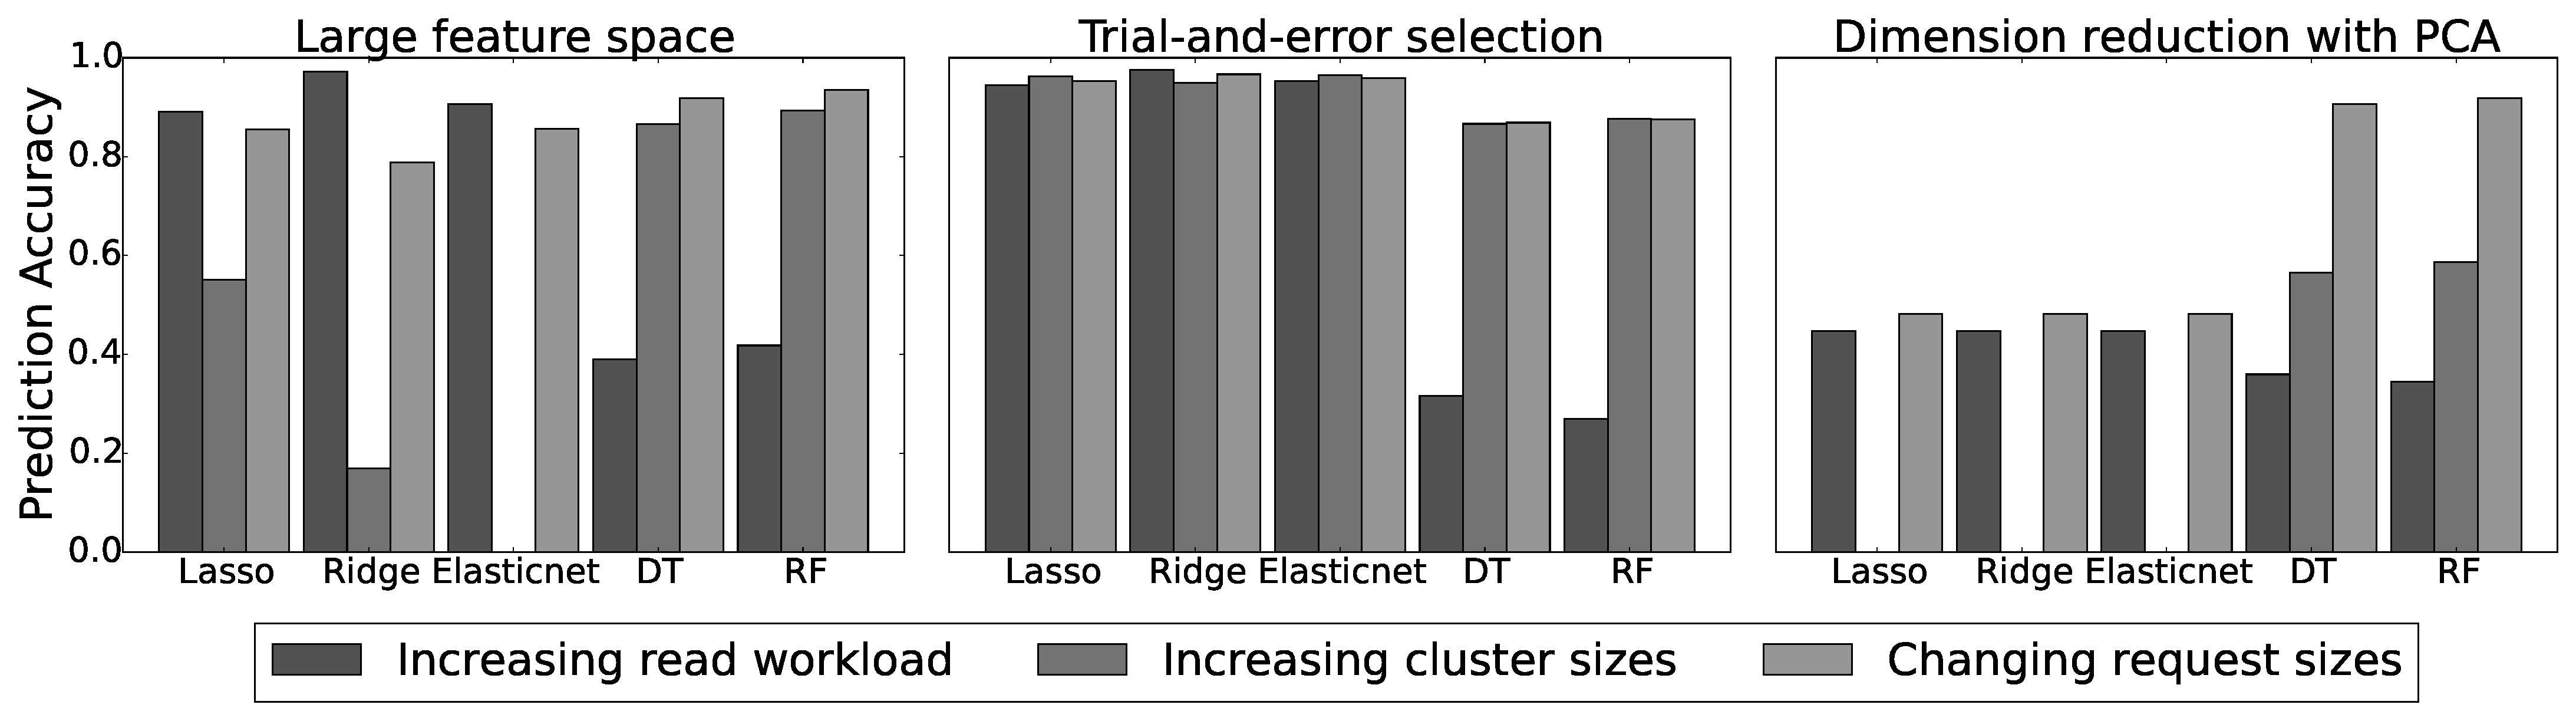
\includegraphics[width=1\textwidth]{figures/challenge_generalization_combined_horizental.eps}
    \caption{Prediction accuracy is inconsistent due to the large feature space.
    Learning methods fail to select the right features in some cases.
    Dimension reduction (PCA with 10 components) does not help in this case.
    In the trial-and-error case, we select a subset of metrics, e.g. \emph{mean(disk.read)}, \emph{sum(network.recv)} and \emph{std(cpu.usr)}.}
    \label{fig:challenge_generalization}
\end{figure*}

Although Hyperparameter tuning, model selection, and 
feature selection have been proposed as potential solutions, it is challenging 
to use them in practice, not to mention the complexity of automating this task. 
PCA (Principle Component Analysis) is another potential solution \cite{Shlens2003}.
PCA transforms original data into a lower dimension while keeping high fidelity.
However, PCA has several limitations. 
First, PCA is not scale invariant.
Not all performance metrics are comparable and therefore, there is no standard way to scale these metrics.
Second, PCA assumes Gaussian distribution in data points; however, many storage workloads have Pareto distribution \cite{Kim2010}.
Third, determining a good number of components is also a challenging task.
In our case, PCA does not address the problems.
In fact, \myfigure{\ref{fig:challenge_generalization}} shows that it can further degrade prediction accuracy.

\subsection{A Two-Level Approach}

Instead of performing feature selection or dimension reduction, we propose a generic two-step approach that can improve the consistency of prediction accuracy. 
In the first step, we use some heuristic methods to filter out irrelevant features.
Then, in the second step, we apply machine learning algorithms to build performance models with the reduced feature set.
The intuition behind this idea is that it is difficult to determine the most important performance features but it is relatively easy to eliminate unimportant features.
For example, the features which are not in the top 100 list after step one can be labeled as unimportant features.
% \section{The Inside-Out Design}
\label{sec:methodology}
%\rp{Chin: In the previous section, you say ``As we will explain in Section V-A, we use 32 low-level performance 
%metrics collected with dstat''. This section does not say anything about 32 metrics. Please mention them here. 
%I think we need to write this section in a much better way. You should clearly explain the steps: something like: We collect 32 
%low level system metrics from each VM (either give the list or mention just the few) every x seconds. Then say we take mean, std, sum and 5\% of each 
%of these 32 metrics for every moving window of xxx seconds. Then explain why we use moving window. then say that for training and validation purposes, 
%we measure the end-to-end performance metrics (IOPS, throughput, and latency) using cosbench every x seconds. Then we take average, xxx, xxx etc. 
%of these metrics ...I think you get the point now, right? We have to clearly explain what we exactly did. }
In this section, we present the design of Inside-Out.
We also discuss the trade-offs among a set of representative machine learning algorithms
and propose a two-step learning technique for mitigating overfitting problems.



\subsection{Collecting and Pre-Processing Low-Level Metrics}
\label{sec:data_preprocessing}

Inside-Out collects general, low-level system metrics from individual machines running the distributed storage service.
However, the raw collected data suffers from various problems due to inefficiency of data collectors, system clock skews,
incomparable data formats, workload outliers, bursty system anomalies, \etc
The noisy data can lead to unstable and 
inaccurate performance models. 
Inside-Out performs a series of data pre-processing functions to address these issues.

%\rp{The goal of this step is to remove unwanted characteristics of the collected data, such as
%workload outliers, system clock deviation, incomparable data format, etc.
%}


%Data preprocessing is a preparation step before training a model.


\subsubsection{Monitoring storage components}
We collect low-level system metrics of the underlying operating system to capture resource utilization 
(\eg cpu, memory, disk and network usage).  
The low-level performance metrics are sampled with one-second granularity.
Such data can be collected from \textit{libvirt}, Ganglia, instrumented hypervisors \cite{Koh2007} and \textit{Ceilometer} in OpenStack.
We use  \emph{dstat} monitoring tool (with option: -tcly -mg --vm -dr -n --tcp --float) to collect these data.


%This step helps us eliminate unwanted characteristics of the collected data, such as
%high variation due to workloads, uncertainty originated by physical hardware, 
%system clock deviation, incomparable data format, etc.
%For the collected performance data, fluctuating metrics, time synchronization and feature transformation for a distributed system are the major challenges.

%\subsubsection{Smoothing monitored data}
\subsubsection{Data smoothing}
%
Building a performance model with data collected at one-second granularity is challenging because 
system data can exhibit high variance at small time scales, \eg due to dynamic/bursty workloads and interference among co-located tenants.
Furthermore, the storage IO operation needs to pass through a series of software layers 
between the storage client and the back-end raw physical storage device. 
The long storage IO path can introduce high variability in resource utilization at smaller time scales. 
For example, HDFS and Ceph both replicate data blocks across storage nodes distributed in physically disjoint 
servers, racks or even datacenters.
To address the uncertainties due to complex IO path spanning several software layers, 
we compute the moving average of the collected performance data.
We have empirically found that one-minute window for processing the moving average is sufficient to 
eliminate outliers from the raw data.
%we use moving averages to construct a stable prediction model.
%We choose one-minute windows for moving average since we have empirically found 60-second moving averages to smooth out raw data sufficiently, without 
%compromising data quality, in order to yield stable and accurate performance models.
%A fine granularity, at lease 15 seconds, is also desirable from our experience.

%RP: Chin, I commented the following line becuause it looks too vague. If you want to clarify this, 
%we can restate in a better way. 
%and the uncertainty come from the interaction between software and hardware components.
%We use moving average to smooth the collected performance data for stable prediction model.
%\rp{Chin: Please explain ``moving average of xxx'', ``why 15 seconds is a desirable window''. These aspects need to be mentioned 
%in a clear manner, not in a handwavy way.}
%We use moving average to construct a stable prediction model.
%Based on our data collected from our internal testbed, 
%it is desirable to use a window greater than 15 seconds. 
%From our experience, a window greater than 15 seconds shows stable results.
%One reason is that a storage request can last longer than 10 seconds for accessing large objects (or files).

\subsubsection{Timestamp alignment}
Proper time synchronization among participating servers is essential to correlate data collected from those servers. 
We use NTP for time synchronization.
The average timestamp of all nodes is taken as the basis for time alignment.

\subsubsection{Feature transformation for a distributed storage system}
%
As mentioned earlier, elasticity is an important feature of SDS, since it needs to adjust its size based on storage demand. 
%The built prediction model needs to be able to predict end-to-end performance at different system scales.
Thus our model must accurately predict end-to-end performance at arbitrary deployment scales.
However, the data collected from different scales may have different dimensions. 
For instance, Ceph with 10 Object Storage Servers (OSDs) generates 10 copies of low-level performance metrics, 
while Ceph with 5 OSDs generates fewer data points. This makes it hard to train and build a unified model.
As mentioned in Section~\ref{sec:feaatures_for_distributed_system}, we use \emph{mean, sum, std, and 5\%} statistical 
variables to capture 
different types of workload distribution such as
\emph{hotspot}, \emph{load imbalance}, and \emph{aggregate performance}.

%To achieve the goal, we need to make sure the dimension of data, collecting from different system configurations are comparable.
%As suggested in Section~\ref{sec:feaatures_for_distributed_system}, our feature transformation describes a distributed system as in one of the four conditions: load-balancing, non-load-balancing, hotspot and the aggregate workload.
%As suggested in Section~\ref{sec:feaatures_for_distributed_system}, our feature transformation process 
%takes four conditions into account: load-balancing, non-load-balancing, hotspot and the aggregate workload.

In summary, Inside-Out collects 32 raw low-level system metrics with one-second granularity.
Inside-Out applies proper time alignment and moving average with one-minute windows for stabilizing performance data.
Then it calculates \emph{mean}, \emph{std}, \emph{sum} and \emph{5\%} of individual metrics collected from multiple machines.
This ensures that our performance model can accept input data for systems with varying scales of deployment, 
while preserving important characteristics of a distributed storage system.
For training and validation purposes, 
we measure end-to-end performance metrics (IOPS, throughput, and latency) every 5 seconds using COSbench \cite{cosbench}, and take average over the one-minute window.
Next, we describe how we build end-to-end performance models in order to capture the relationship between low-level system metrics and end-to-end throughput and IOPS.

%Lastly, we transform low-level performance metrics to create comparable dataset while preserving characteristics 
%of a distributed storage system, using the feature transformation specified in Figure~\ref{fig:feature_types}.

%In summary, we use a 60-seconds window to smooth performance data, and proper time alignment has applied to the monitored performance data.
%\mra{Chin, what did you use to transform the data? average? It would be good if we can briefly state how we transform the data.
%if you already described this somewhere later in the paper, we could forward reference the section.}


\subsection{Exploring Learning Methods}
\label{sec:algorithm_selection}

%We collect time series data composed of low-level system metrics collected from all machines running the distributed storage system. 
%At each sampling time (every $t$ seconds), a low-level performance snapshot of a running distributed storage system is \rp{obtained from} the dataset.
%Given a performance snapshot at time $t$ of a running distributed storage, we aim to build a model that predicts the storage's end-to-end performance, e.g. throughput and IOPS.
%The performance snapshot is the low-level performance metrics collected from distributed storage nodes.

Our goal is to build a model that accurately predicts end-to-end throughput and IOPS by analyzing only the low-level metrics of a distributed storage system.
We explore several algorithms, including statistical regression \cite{Fron2004, hastie2005}, 
decision tree learning and random forests learning \cite{hastie2005,Wang2004}.
For statistical regression, we mainly focus on linear regression techniques, 
which can be extended to support non-linear regression by expanding features that simulate, 
for example, quadratic terms \cite{Kundu2010}.
We did not find this necessary in our application and exclude the discussion.

%\subsubsection{Lasso}
%\textit{Lasso\footnote{Least Absolute Shrinkage and Selection Operator}} 
% remove the full name above
\textit{Lasso} 
is a least square linear regression technique with L1-norm regularization.
The L1 penalty function leads to a sparse solution, which has an effect of restricting 
the number of selected variables.
This property is useful for figuring out important features, especially 
when the number of variables or features is large.
%
%\subsubsection{Ridge}
\textit{Ridge} is similar to Lasso but instead uses L2-norm regularization, 
which has the effect of group selection of variables.
This property does not restrict the number of variables selected by the prediction model 
and therefore, the prediction accuracy might degrade and become inconsistent 
%when the feature space is large.
when the number of input features to the training model is large. 
%when we use a small number of features out of much larger feature space.
%\mra{Chin, I modified the previous sentence. Check if it is ok with you.}
%
%\subsubsection{Elastic Net}
\textit{Elastic Net} combines both advantages---it does group selection while enforcing sparsity.
Based on our data set, Lasso and Elastic Net have similar prediction performance, and Ridge shows larger variance.
%
The \textit{Decision Tree} (DT) learning uses a top-down approach and recursively partitions data to fit target values.
The tree-based model is easy to interpret and scales well to large datasets.
\textit{Random Forests} (RF) is an ensemble method that uses multiple decision trees~\cite{hastie2005}.
%In practice, it is accurate, efficient, and more robust compared to a single decision tree.
RF improves a single decision tree in many ways, e.g., accuracy, efficiency, and robustness.
%Due to space limit, please refer to \cite{hastie2005} for detailed description.

To summarize, linear regression models assume a linear relationship and might oversimplify the storage behavior. 
Nonetheless, it has the potential to exhibit better generalization for extrapolating performance prediction 
for the unknown behavior case (the pattern not included in the training dataset).
On the other hand, the tree-based learning can achieve good model accuracy (perfectly fits the training data), 
but it can easily lead to overfitting problems.
Its prediction accuracy decreases, for example,
under different storage workloads,
as shown in \myfigure{\ref{fig:challenge_generalization}}.


\subsection{Two-level Training}
\label{sec:auto_feature_selection}

%As discussed in Section~\ref{sec:non-deterministic}, 
The fundamental challenge 
in building an effective prediction model from a large set of features is the overfitting problem.
One way to address this problem is to perform manual feature selection.
However, this approach is problematic because the right set of features depend on application types, 
deployment topology, resource constraint, etc.

Instead, we propose a two-level training process that filters out irrelevant features in the first step 
and then builds models by using the reduced set of features in the second step.
To this end, Inside-Out pipelines Ridge and Lasso together, where Ridge filters features in 
coarse-granularity and then Lasso builds the prediction model.
We choose Ridge as the filtering algorithm because it is not a sparse solution and considers all features. 
We then apply exhaustive grid search to find the optimized score for important features.
We use $\alpha \times$ \textit{median(coefficients)} derived from Ridge as the threshold.

For comparison, we consider Decision Tree with Lasso (Auto-DTL) and RandomForest with Lasso (Auto-RFL).
Our evaluation shows Inside-Out outperforms consistently across all prediction cases, 
and boosts prediction accuracy in several scenarios, where the linear regression models 
fail to generalize the behavior of a distributed storage system.
We also experimented by using Lasso and Elastic Net as the filter algorithm but did not find comparable performance with Inside-Out.
%Beside, we also evaluated Lasso and used Elastic Net as a filter algorithm and 
%found they are not comparable with Auto-RL.
%\mra{this sentence is a little confusing..}
%We will leave them as future work to further study the major difference.

Inside-Out uses the following pseudo code to generate an end-to-end performance model.
In practice, we set $k$ to $10$ for stable prediction results.
The data processing part is explained in previous sections.
Features are automatically selected using the Ridge algorithm
with multiple thresholds.
We vary $\alpha$ from $0.1, 0.2, ..., 1.0$.
The grid search approach is used to select the best model.


 \begin{algorithm}
 \caption{Inside-Out Model Building}
 \begin{algorithmic}[1]
 \renewcommand{\algorithmicrequire}{\textbf{Input:}}
 \renewcommand{\algorithmicensure}{\textbf{Output:}}
 \REQUIRE low-level performance metrics from distributed nodes
 \ENSURE  an end-to-end performance model
 \\ \textit{Initialisation}
  \STATE $thresholds = \left \{ \alpha_{1}, ... , \alpha_{N} \right \} $\
  \STATE $m1 =$ filtering algorithm $\rightarrow Ridge$
  \STATE $m2 =$ model algorithm $\rightarrow Lasso$
  \STATE $k =$ k-fold cross validation
  \STATE $score = 0$
 \\ \textit{Data preprocessing} (refer to Section~\ref{sec:data_preprocessing})
  \STATE alignment of input data
  \STATE calculate moving average across metrics
  \STATE feature transformation for the distributed scenario
 \\ \textit{Grid Search}
  \FORALL{$t \in thresholds$}
  \STATE $features =$ execute $m1$ with threshold $t$
  \STATE $score, m = $max(crossvalidation($k$, $m2$, $features$))
  \ENDFOR
 \RETURN $m$ with maximum $score$
 \end{algorithmic} 
 \end{algorithm}

% 
\section{Evaluation}
\label{sec:evaluation}

%In this section, we present a comprehensive evaluation of how well Inside-Out can predict end-to-end storage performance (latency, throughput and IOPS) 
%using low-level system metrics for a wide range of SDS environment.
In this section, we present a comprehensive evaluation of Inside-Out.
We demonstrate that Inside-Out can accurately predict end-to-end performance, 
i.e., throughput and IOPS, using low-level system metrics and
is applicable to a wide range of realistic scenarios.

%SDS offers wide flexibility for hosting storage services and in this section, we present comprehensive evalution to study whether low-level performance metrics can accurate end-to-end performance and Inside-Out can be applied for practical use in many SDS senarios.
%All SDS scenarios are listed in Table~\ref{tab:prediction_scenario}.


\subsection{Setup}
\label{sec:dataset}

%We choose Ceph as the storage service running on our SDS platform \cite{ceph}. 
%We use COSBench for measuring the storage performance \cite{cosbench}.
%COSBench supports several object storage protocols, including \textit{librados} used by Ceph. 
We choose Ceph~\cite{ceph} as a target distributed storage service for our evaluation and             
use COSBench~\cite{cosbench} to generate various types of storage workloads.
COSBench supports several object storage protocols, including \textit{librados} for Ceph, and
provides a set of knobs to change storage traffic pattern. 
Table~\ref{tab:cosbench_configurations} lists Ceph and COSBench configurations used in our experiments.
%We collected benchmarking data from three SDS clusters 
%located in a research lab of a major telecommunication company. 

\newcommand{\scenarioMU}{Increasing users}
\newcommand{\scenarioCUB}{Complex usage}
\newcommand{\scenarioCRB}{Complex request}
\newcommand{\scenarioWIB}{Write intensive}
\newcommand{\scenarioRIB}{Read intensive}
\newcommand{\scenarioMWIB}{Medium write intensive}
\newcommand{\scenarioMRIB}{Medium read intensive}
\newcommand{\scenarioMM}{Reconfigure Ceph}
\newcommand{\scenarioSUI}{Scale-up instances}
\newcommand{\scenarioMBS}{Medium network SLO}
\newcommand{\scenarioLBS}{Low network SLO}
\newcommand{\scenarioSON}{Scale out to}
\newcommand{\scenarioSIN}{Shrink in to}
\newcommand{\scenarioMTA}{Case 1 - tenant 1 (250 Mbit)}
\newcommand{\scenarioMTB}{Case 1 - tenant 2}
\newcommand{\scenarioMTAA}{Case 2 - tenant 1}
\newcommand{\scenarioMTBB}{Case 2 - tenant 2}


\newcommand{\spheading}[2][10em]{% \spheading[<width>]{<stuff>}
  \rotatebox{90}{\parbox{#1}{\raggedright #2}}}

\begin{table*}[t!]
  \fontsize{8}{8}\selectfont
  \centering
  \caption{Common scenarios that storage behavior can change in a software-define storage environment}
  \begin{tabularx}{.95\linewidth}{|l|c|c|c|X|}
  \hline
  & \textbf{Scenario} & \textbf{Training Dataset} &  \textbf{Prediction Dataset} & \textbf{Explanation} \\
  \hline
  \multirow{7}{*}[-0.3ex]{\rotatebox[origin=c]{90}{\textbf{Changing Workload}}} & \scenarioMU & \{1, 2\} & \{4\} & The number of client virtual machines running COSBench. \\
  \cline{2-5}
  & \scenarioCUB & \{1, 2, 4, 8\} & \{16, 32\} & The number of threads for all benchmark clients. \\
  \cline{2-5}
  & \scenarioCRB & 512KB & 1-1024KB & The request size (either static or variable) of the workload, configured in COSBench. \\
  \cline{2-5}
  & \scenarioWIB & \{50, 75, 100\} & \{25, 0\} & \multirow{4}{1\linewidth}{The percentage of read operations the workload. The read and write percentages are 100 in total.}\\
  \cline{2-4}
  & \scenarioRIB & \{0, 25, 50\} & \{75, 100\} & \\
  \cline{2-4}
  & \scenarioMWIB & \{0, 50, 100\} & \{25\} & \\
  \cline{2-4}
  & \scenarioMRIB & \{0, 50, 100\} & \{75\} & \\
  \hline
  \hline
  \multirow{4}{*}[-1.7ex]{\rotatebox[origin=c]{90}{{\textbf{Reconfiguration}}}} & \scenarioMM & \{1\} & \{2\} & The number of Ceph monitor daemons.\\
  \cline{2-5}
  & \scenarioSUI & m1.small & m1.medium & The instance type of the virtual machines running Ceph is upgraded to a powerful one.  A m1.small instance has one core and 2GB memory and m1.medium has two cores and 4GB memory.  Note that in this setting, the configuration of disk I/O remains the same.\\
  \cline{2-5}
  & \scenarioMBS & unrestricted & 500 Mbps & The network bandwidth of virtual machines is limited at 500 Mbps.  We use the Linux tool \textit{tc} for network throttling\\
  \cline{2-5}
  & \scenarioLBS & unrestricted & 250 Mbps & Network bandwidth is limited at 250 Mbps.\\
  \hline
  \hline
  \multirow{2}{*}[-0.5ex]{\rotatebox[origin=c]{90}{\textbf{Elasticity}}} & \scenarioSON { \textit{n}} & \{4, 6, 8, 10\} & \{20, 30, 40\} & The total number of Ceph OSDs.  Note that each OSD is running in a virtual machine and different OSDs can run on the same physical servers (10 servers in total). \\
  \cline{2-5}
  & \scenarioSIN { \textit{n}} & \{20, 30, 40\} & \{4, 6, 8, 10\} & Similar to the above, but the cluster size is decreased. \\
  \hline
  \end{tabularx}
  \label{tab:prediction_scenario}
\end{table*}

\begin{table}[!htbp]
\centering

\caption{The evaluated applications. In total, there are 30 applications and 107 workloads measured on Hadoop 2.7, Spark 1.5 and Spark 2.1.}
\label{tab:dataset}
\resizebox{.95\linewidth}{!}{%
\begin{tabular}{@{}p{2.5cm}p{14cm}@{}}
\toprule
\textbf{Application} & \textbf{Description} \\ \midrule
\multicolumn{2}{l}{\noindent{\textbf{Micro Benchmark}}} \\
sort & Sorts text input data, generated by RandomTextWriter in Hadoop. \\
terasort & A standard Hadoop benchmark. Data is generated from TeraGen. \\
pagerank & The PageRank algorithm. Hyperlinks follow the Zipfian distribution. \\
wordcount & Counts the frequency of words that generated by RandomTextWriter.  This is a typical MapReduce job. \\ \midrule
\multicolumn{2}{l}{\textbf{OLAP}} \\
aggregation & A Hive query performing aggregation. \\
join & Implement the join operation in Hive \\
scan & Implement the scan operation in Hive \\ \midrule
\multicolumn{2}{l}{\textbf{Statistics Function}} \\ 
chi-feature & Chi-square Feature Selection. \\
chi-gof & Chi-Square Goodness of Fit Test. \\
chi-mat & Chi-square Tests for identity matrix. \\
spearman & Compute Spearman's Correlation of two RDDs. \\
statistics & Generate column-wise summary statistics. \\
pearson & Compute the Pearson's correlation of two series of data. \\
svd & Singular Value Decomposition, a fundamental matrix operation for finding approximate solutions.\\
pca & Principal Component Analysis for dimension reduction. \\
word2vec & Generate distributed vector presentation of words according to distance. \\ \midrule
\multicolumn{2}{l}{\textbf{Machine Learning}} \\
classification & Implement the generalized linear classification model. \\
regression & Generalized Linear Regression Model. \\
als & The Alternating Least Squares algorithm, implemented in spark.mllib. It is a collaborative filtering algorithm used for product recommendation. \\
bayes & Implements the Naive Bayes algorithm for the multiclass classification problem. Input documents are generated from /usr/share/dict/linux.words.ords. \\
lr & A popular algorithm for the classification problem. \\
mm & Matrix multiplication with configurable row, column and block sizes.\\
d-tree & A greedy algorithm for classification and regression problems. \\
gb-tree & Gradient Boosted Tree, an ensemble learning method for classification and regression problems. \\
df & The Random Forest algorithm for classification and regression problems. \\
fp-growth & The FP-growth algorithm to mine frequent pattern in large-scale dataset. \\
gmm & Gaussian Mixture Model is a clustering algorithm that uses k Gaussian distributions to find the k clusters. \\
kmeans & K-means is a common clustering algorithm that finds k cluster centers. \\
lda & Latent Dirichlet allocation is a clustering algorithm that infers topics from a collection of text documents. \\
pic & Power iteration clustering is a scalable algorithm for clustering. \\ \bottomrule
\end{tabular}
}
\end{table}



We collected benchmarking data from an OpenStack-based SDS platform.
The cluster has 16 machines, and
each machine has 16 cores, 24GB memory and 250GB disk space.
Each machine has 1Gbps network interface connected to a 10Gbps switch.
The dataset is collected from about 5300 benchmark runs. The total dataset is composed of about 15.2 million records, each of which is 
a vector of 32 low-level performance data.
The end-to-end performance data collected from COSBench contains 
3 million records. 
The combined dataset is about 24GB, collected over two weeks. 

%[comment: please briefly describe cluster A/B/C in text as well (using the table II's content). we need to be kind.]
%The dataset is collected from 8300 benchmark runs in total; 5300 runs on \textit{Cluster A}, 
%1500 runs on \textit{Cluster B}, and 1500 runs on \textit{Cluster C}.
%The total number of records of low-level performance data is more than 18 million 
%and each record is a vector with 32 metrics.
%Our resulting dataset is made up of 18 million records, each of which is 
%a vector of 32 low-level performance data.}
%The number of records for \chin{end-to-end} performance data collected from COSBench contains 
%\chin{3.6 million} records, which is one-fifth of the low-level records.
%The combined dataset is about 34GB, and is worth about two-week measurements in total.
%All raw performance data can be found at \chin{http://xxx.xxx}.
%RP: We cannot publish any data without approval from AT&T.


\subsection{The Comparison Method}
Our goal is to find a function $f(X_t)$ that predicts the end-to-end performance, where $X_t$ is a vector that describes the internal status at time $t$ of a distributed storage service.
We say a model is accurate if $f(X_t)=\hat{y_t} \simeq y_t$, where $y_t$ is the ground truth (measured at the client side) and $\hat{y_t}$ is the predicted values.
To interpret performance models, we are interested in four indicators:
1) the overall prediction accuracy,
2) the goodness-of-fit,
3) the consistency across diverse scenarios and
4) the consistency across prediction instances.

First, we use mean absolute percentage error (MAPE) to compute prediction accuracy as 
\setlength{\abovedisplayskip}{0pt} \setlength{\abovedisplayshortskip}{0pt}
%\begin{center}
\begin{equation} \label{eq:prediction_accuracy}
max(1 - \frac{\sum_{t=1}^{n} {|\frac{y_t - \hat{y_t}}{y_t}|}}{n}, 0)
\end{equation}
%\end{center}
where $n$ is the length of the observation period.
%For example, for a three-minute measurement period with one-minute sampling window, 
%if the measured performance values are $[10, 20, 30]$ and the predicted values are $[9, 18, 33]$, the average prediction accuracy is $90\%$.
We restrict the scope of prediction accuracy between $0$ to $1$ because the prediction accuracy can be negative (e.g. when $y_t$ is small).

Second, we use the coefficient of determination $R^2$ to interpret \emph{Goodness-of-Fit}, which is less than or equal to one \cite{Noorshams2013}.
Third, we examine whether a performance model can present consistent prediction in various SDS scenarios.
Last, we further analyze the probability density function of prediction decisions for different categories of prediction scenarios.

We consider prediction of throughput and IOPS for both read and write operations, and use the following terms $TP_r$, $TP_w$, $OP_r$ and $OP_w$ for read 
throughput, write throughput, read IOPS and write IOPS, respectively.



\subsection{Baseline: Prediction Performance on Static Deployment}
%

We evaluate prediction accuracy of Inside-Out under a variety of scenarios 
with different storage workloads and configurations
listed in Table~\ref{tab:prediction_scenario}.
In this subsection, we focus on a static deployment scenario with one storage tenant 
running on a distributed Ceph storage service that does not expand or shrink in terms 
of number of VMs used for running Ceph.
Later, we evaluate more challenging scenarios 
in which the Ceph cluster expands or shrinks based on user demand,
and storage traffic of multiple tenants interfere with each other.

%with the Ceph cluster expanding or shrinking based on user demand, 
%and multiple tenants interfering with each others storage traffic. 
%shows various scenarios where the prediction dataset differs from the training dataset.



\vspace{1ex}
%\subsection{Changing Workload}
\subsubsection{Can Inside-Out handle diverse workloads?}
\label{sec:changing_workload}

\begin{figure}
    \centering
    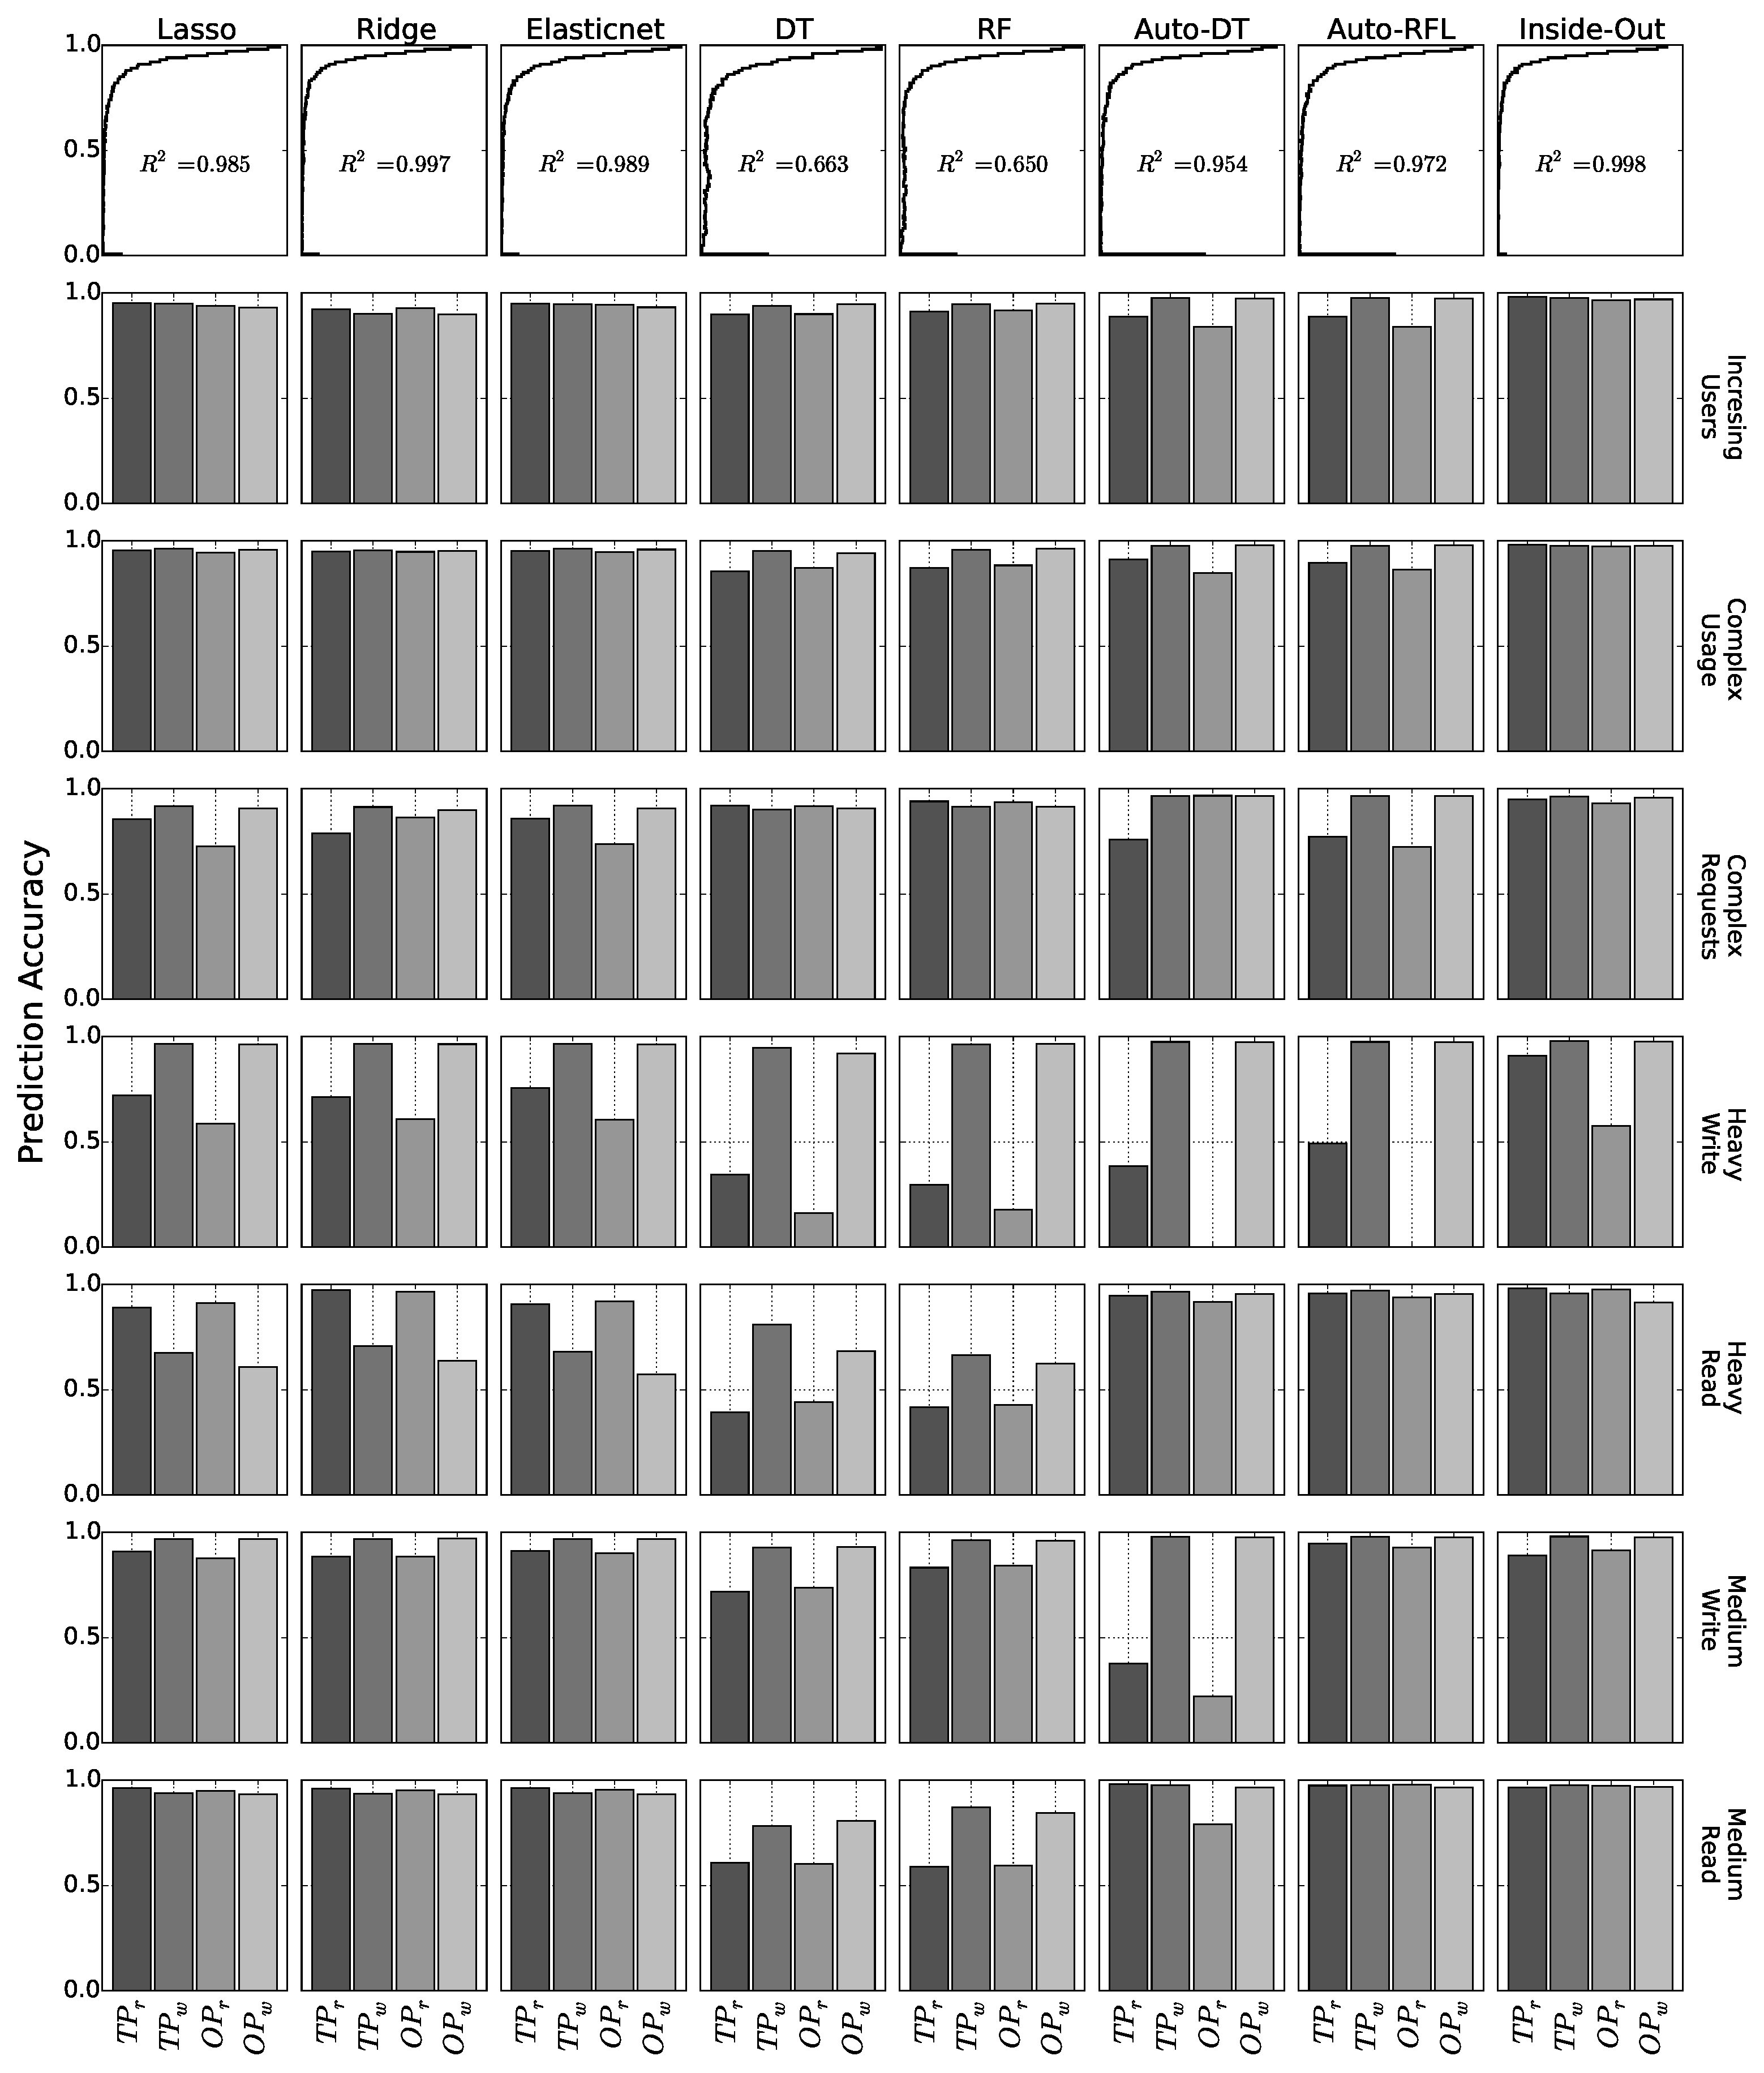
\includegraphics[width=0.9\textwidth]{Chapter-InsideOut/figures/unseen_workload_all_new.eps}
    \caption{Analysis of performance models with diverse workloads. Each bar is the average prediction accuracy. The top row is the probability density function of prediction accuracy for each performance model.}
    \label{fig:changing_workload}
\end{figure}

%\hfill\break

An SDS application needs to handle various request volumes, object/file sizes and different ratios of read/write workloads.
%In practice, it is difficult to obtain a training dataset that includes all access patterns.
First we examine whether Inside-Out can achieve accurate and consistent predictions when workload changes.


\paragraph*{Changing user behavior}
%\textbf{Changing user behavior.}

We increase the number of concurrent clients to stress the Ceph cluster.
%We push the Ceph cluster to a certain limit by increasing the parallelism of clients.
The \emph{\MakeLowercase{\scenarioMU}} scenario changes the number of COSBench clients and the \emph{\MakeLowercase{\scenarioCUB}} scenario increases the worker threads of each client.
As shown in \myfigure{\ref{fig:changing_workload}}, all prediction models perform well. The linear regression technique performs slightly better than the tree-based learning.
The linearly increasing load is well captured by linear models because of proportional change in low-level metrics.
When we switch to the \emph{\MakeLowercase{\scenarioCRB}} scenario, the variable request size slightly changes the behavior of Ceph, affecting prefetching and caching. 
We observe that the linear regression methods (Lasso, Ridge and Elastic Net) show drops in accuracy, e.g. 20\% in the $OP_r$ case; however, Inside-Out 
maintains good accuracy. 
The tree-based learning shows comparable predictions (5-10\% lower) with Inside-Out in these settings.



%\textbf{Complex request behavior.}
%Next, we change the workload from a constant IO request size to variable size.
%In this case, Inside-Out slightly improves the prediction accuracy over Lasso, %and outperforms the three linear models.
%Auto-DT and Auto-RFL show inconsistent prediction result with about 15\% %degradation of accuracy, comparing with the best case.
%One possible expalantion is that some important features filtered by DT and RF 
%are removed.
%Lasso and Elastic Net encounters accuracy drop in the read IOPS prediction


\paragraph*{Varying I/O pattern}

%The workload is a strong performance factor to a storage system \cite{Noorshams2013}.
%The read performance, for example, is affected by the amount of concurrent read or write operations.
Next, we consider workloads with different ratios of read to write operations.
\myfigure{\ref{fig:changing_workload}} shows that varying workload poses a big challenge to performance models. 
The linear regression methods (Lasso, Ridge and Elastic Net) present better prediction accuracy than tree-based models (DT, RL).
In addition, we observe that several models make poor predictions of $TP_r$ and $TP_r$.
The reason is that read behavior is largely affected by \textit{cache}, and large read variance contributes to low prediction accuracy.
Inside-Out performs consistently well, whereas the three linear regression techniques show accuracy drops.
One exception is the $OP_r$ prediction in the \textit{write-intensive} scenario even though $TP_r$ prediction is accurate.
As we will show later in Section~\ref{sec:online_learning}, \emph{over- and under-predictions} cause such behavior. 
The self-learning property of Inside-Out improves its prediction accuracy as it keeps learning the new storage behavior.


\begin{figure}
    \centering
    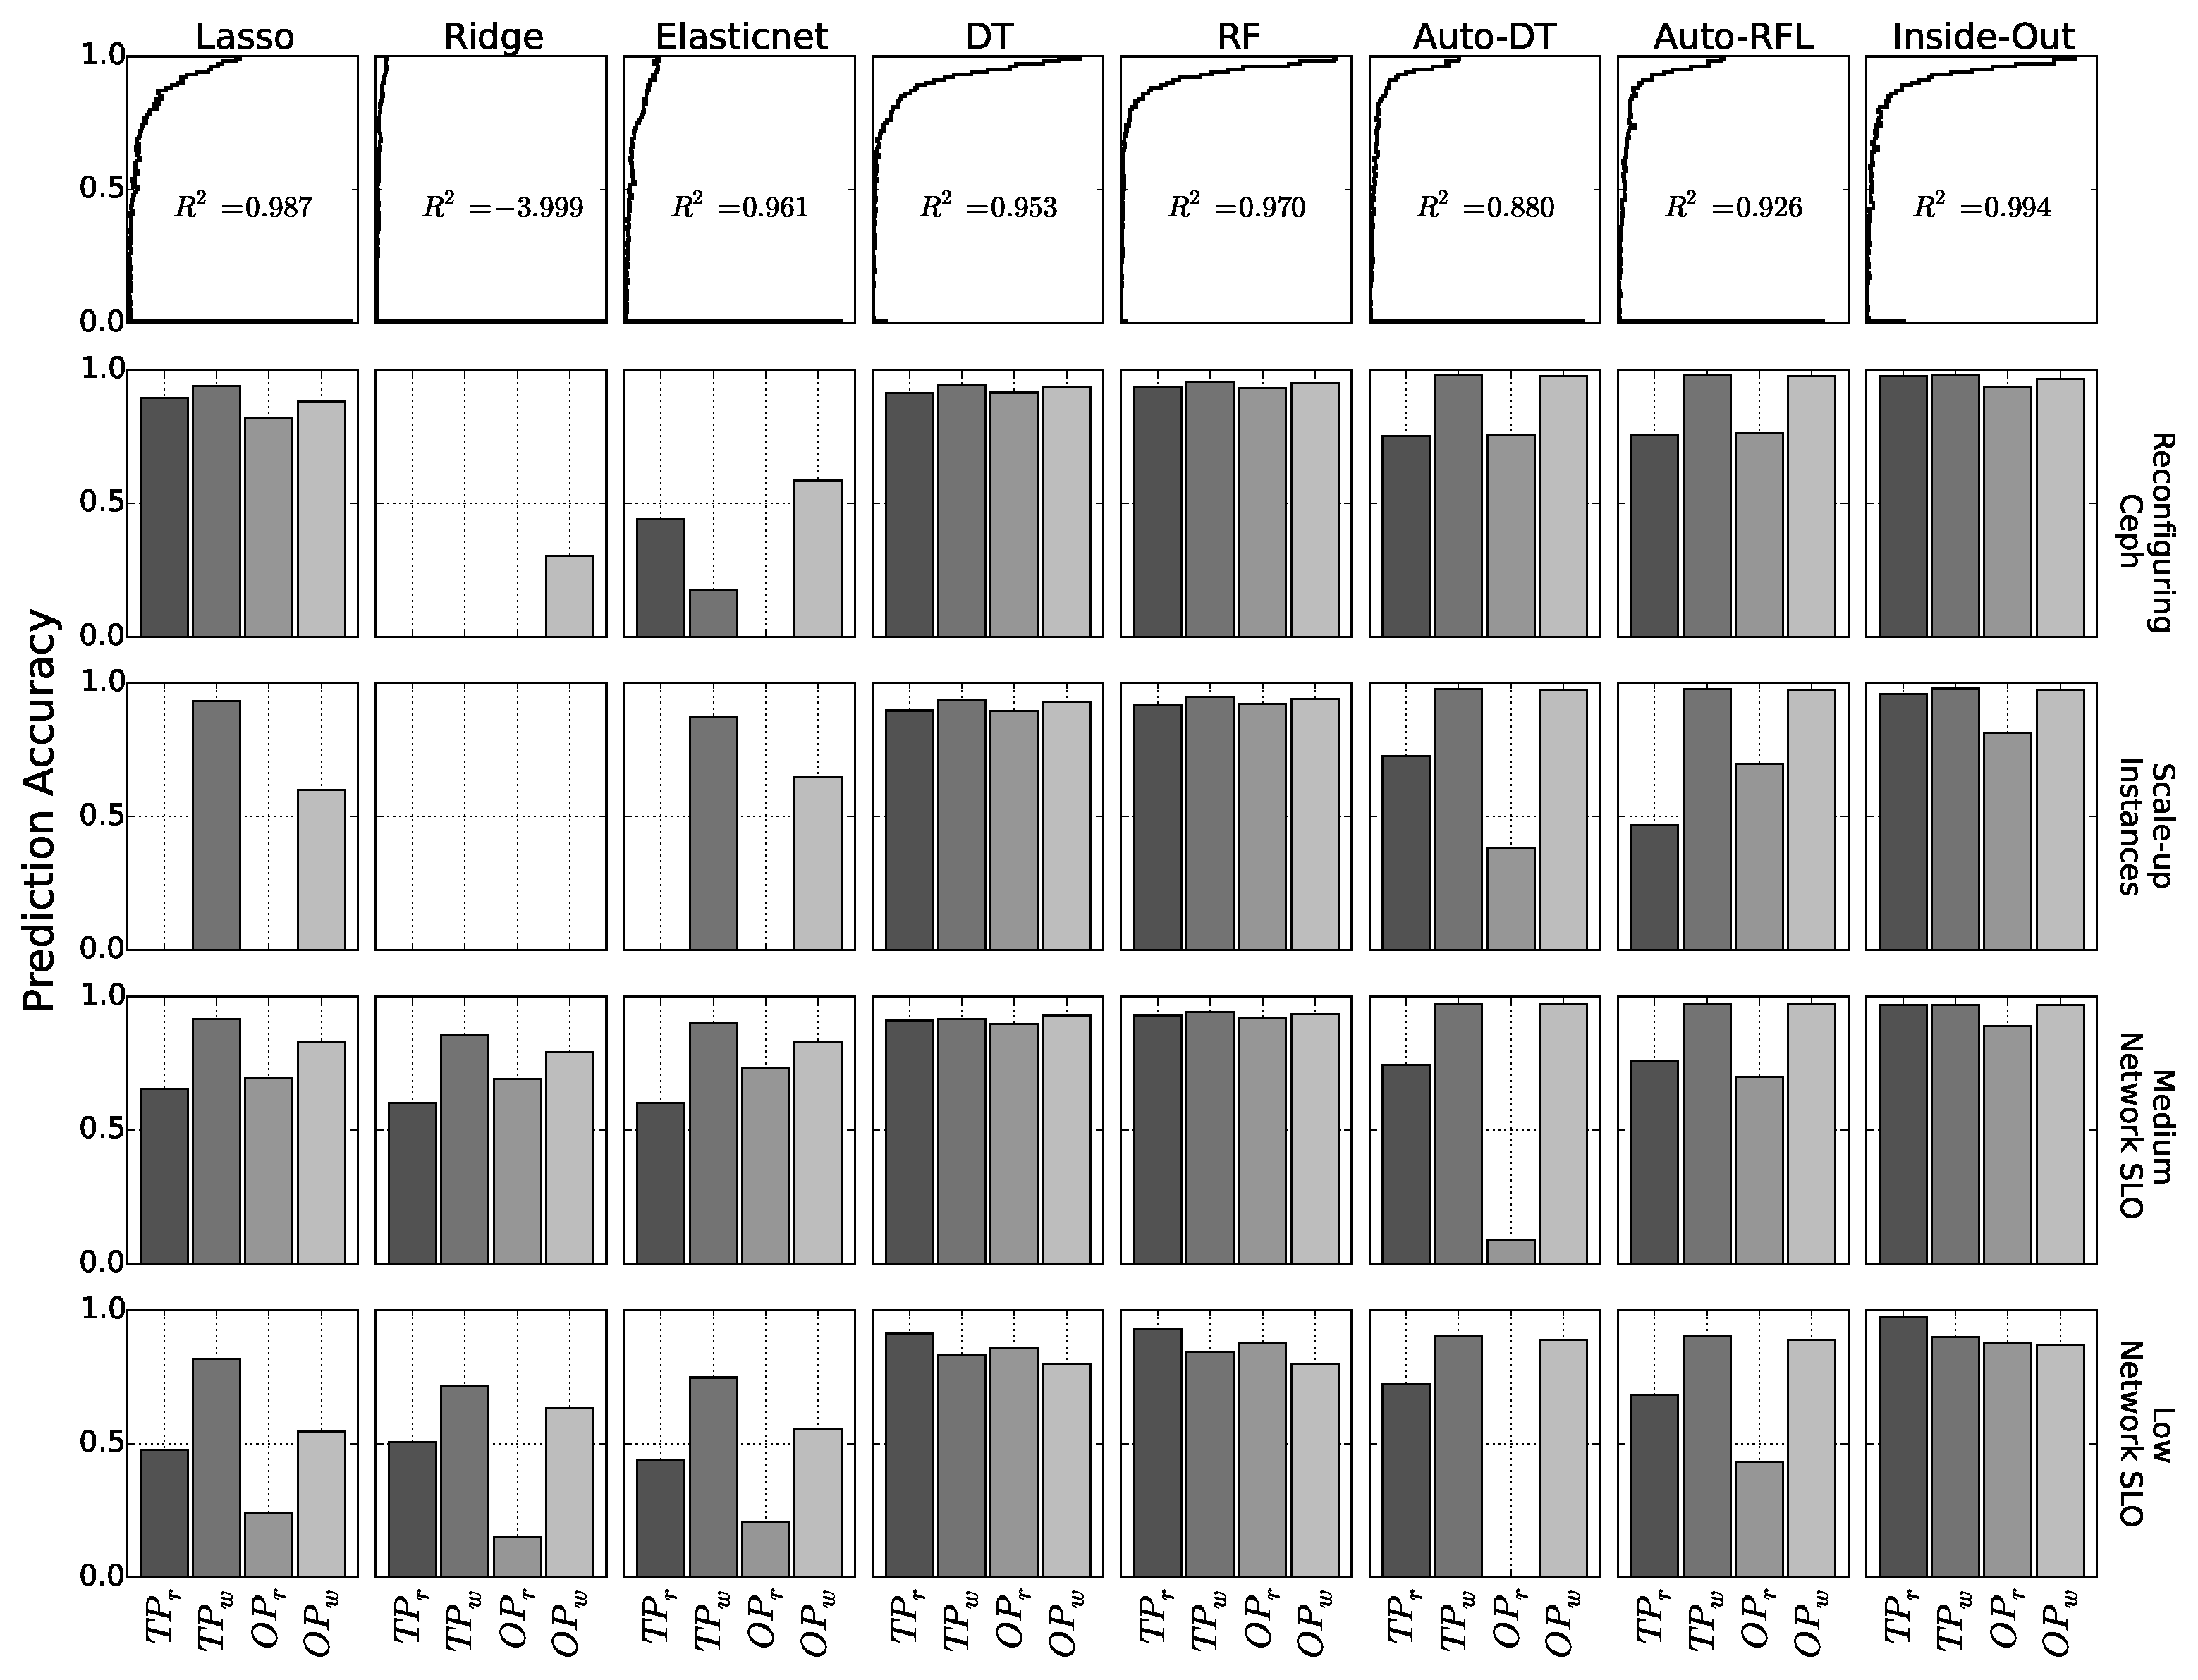
\includegraphics[width=0.9\textwidth]{Chapter-InsideOut/figures/unseen_configuration_all_new.eps}
    \caption{Comparison of performance models when the storage service is reconfigured: Ceph, VMs and network SLOs}
    \label{fig:reconfiguring_storage}
\end{figure}


\paragraph*{Summary}
The linear regression models achieve high prediction accuracy, great goodness-of-fit ($>0.98$) and consistency in prediction 
for many instances (see the distribution of prediction accuracy in \myfigure{\ref{fig:changing_workload}}), but they 
are not consistent across all prediction scenarios.
Inside-Out achieves good prediction accuracy across all cases consistently because the two-level approach 
filters out many irrelevant features in the first step, thereby presenting a smaller relevant feature space to the second step. 
The tree-based learning methods (DT and RF) do not show consistent prediction across all scenarios.
Auto-DT and Auto-RFL, which use DT and RF as the filter algorithms, are not as consistent as Inside-Out.

\vspace{1ex}

%\subsubsection{Reconfiguring Storage}
\subsubsection{Can Inside-Out handle different system configurations?}
\label{sec:unseen_configuration}

We study whether low-level metrics can capture the storage behavior when it is reconfigured by tenants. The results are reported in \myfigure{\ref{fig:reconfiguring_storage}}.


\textbf{Reconfiguring Ceph.}
The first change is to add one extra Ceph monitor daemon. %\chin{which increases the capability to handle a large number of clients.}
Ridge and Elastic Net fail to generate consistent predictions, but Lasso is able to achieve around 80\% to 90\% prediction accuracy.
DT, RF and Inside-Out have very close prediction accuracies, but Auto-DRL and Auto-RFL perform slightly worse in predicting $TP_r$ and $OP_r$.

\textbf{Scale-up instances.}
Increasing CPU and memory allocation to Ceph VM instances improves Ceph's ability to handle more requests.
In this test, we change the instance type from m1.small (1 vCPU, 2GB memory) to m1.medium (2 vCPUs, 4GB memory).
The linear models are unable to predict $TP_r$ and $OP_r$, but Inside-Out's two-level learning performs well by avoiding the overfitting problem. 

\textbf{Network SLOs.}
Here we consider the case where the amount of network bandwidth allocated to Ceph VMs is limited. 
We use Linux network throttling tool \textit{tc} to limit network bandwidth at 500 Mbps and 250 Mbps for medium and low bandwidth SLOs, respectively.
We observe that linear models without the two-level method do not show comparable prediction accuracy across both throughput and IOPS predictions.
The tree-based learning models, on the other hand, achieve 80\% to 90\% accuracy, comparable to Inside-Out.


\textbf{Summary.}
Tree-based learning (DT, RF) models demonstrate promising prediction in terms of prediction accuracy and consistency.
Lasso, Ridge and Elastic Net show inconsistent behavior in the above four scenarios.
Inside-Out, on the other hand, provides consistent predictions and improves Lasso, from 23.9\% to 87.6\% in the extreme case.


\begin{figure}
    \centering
    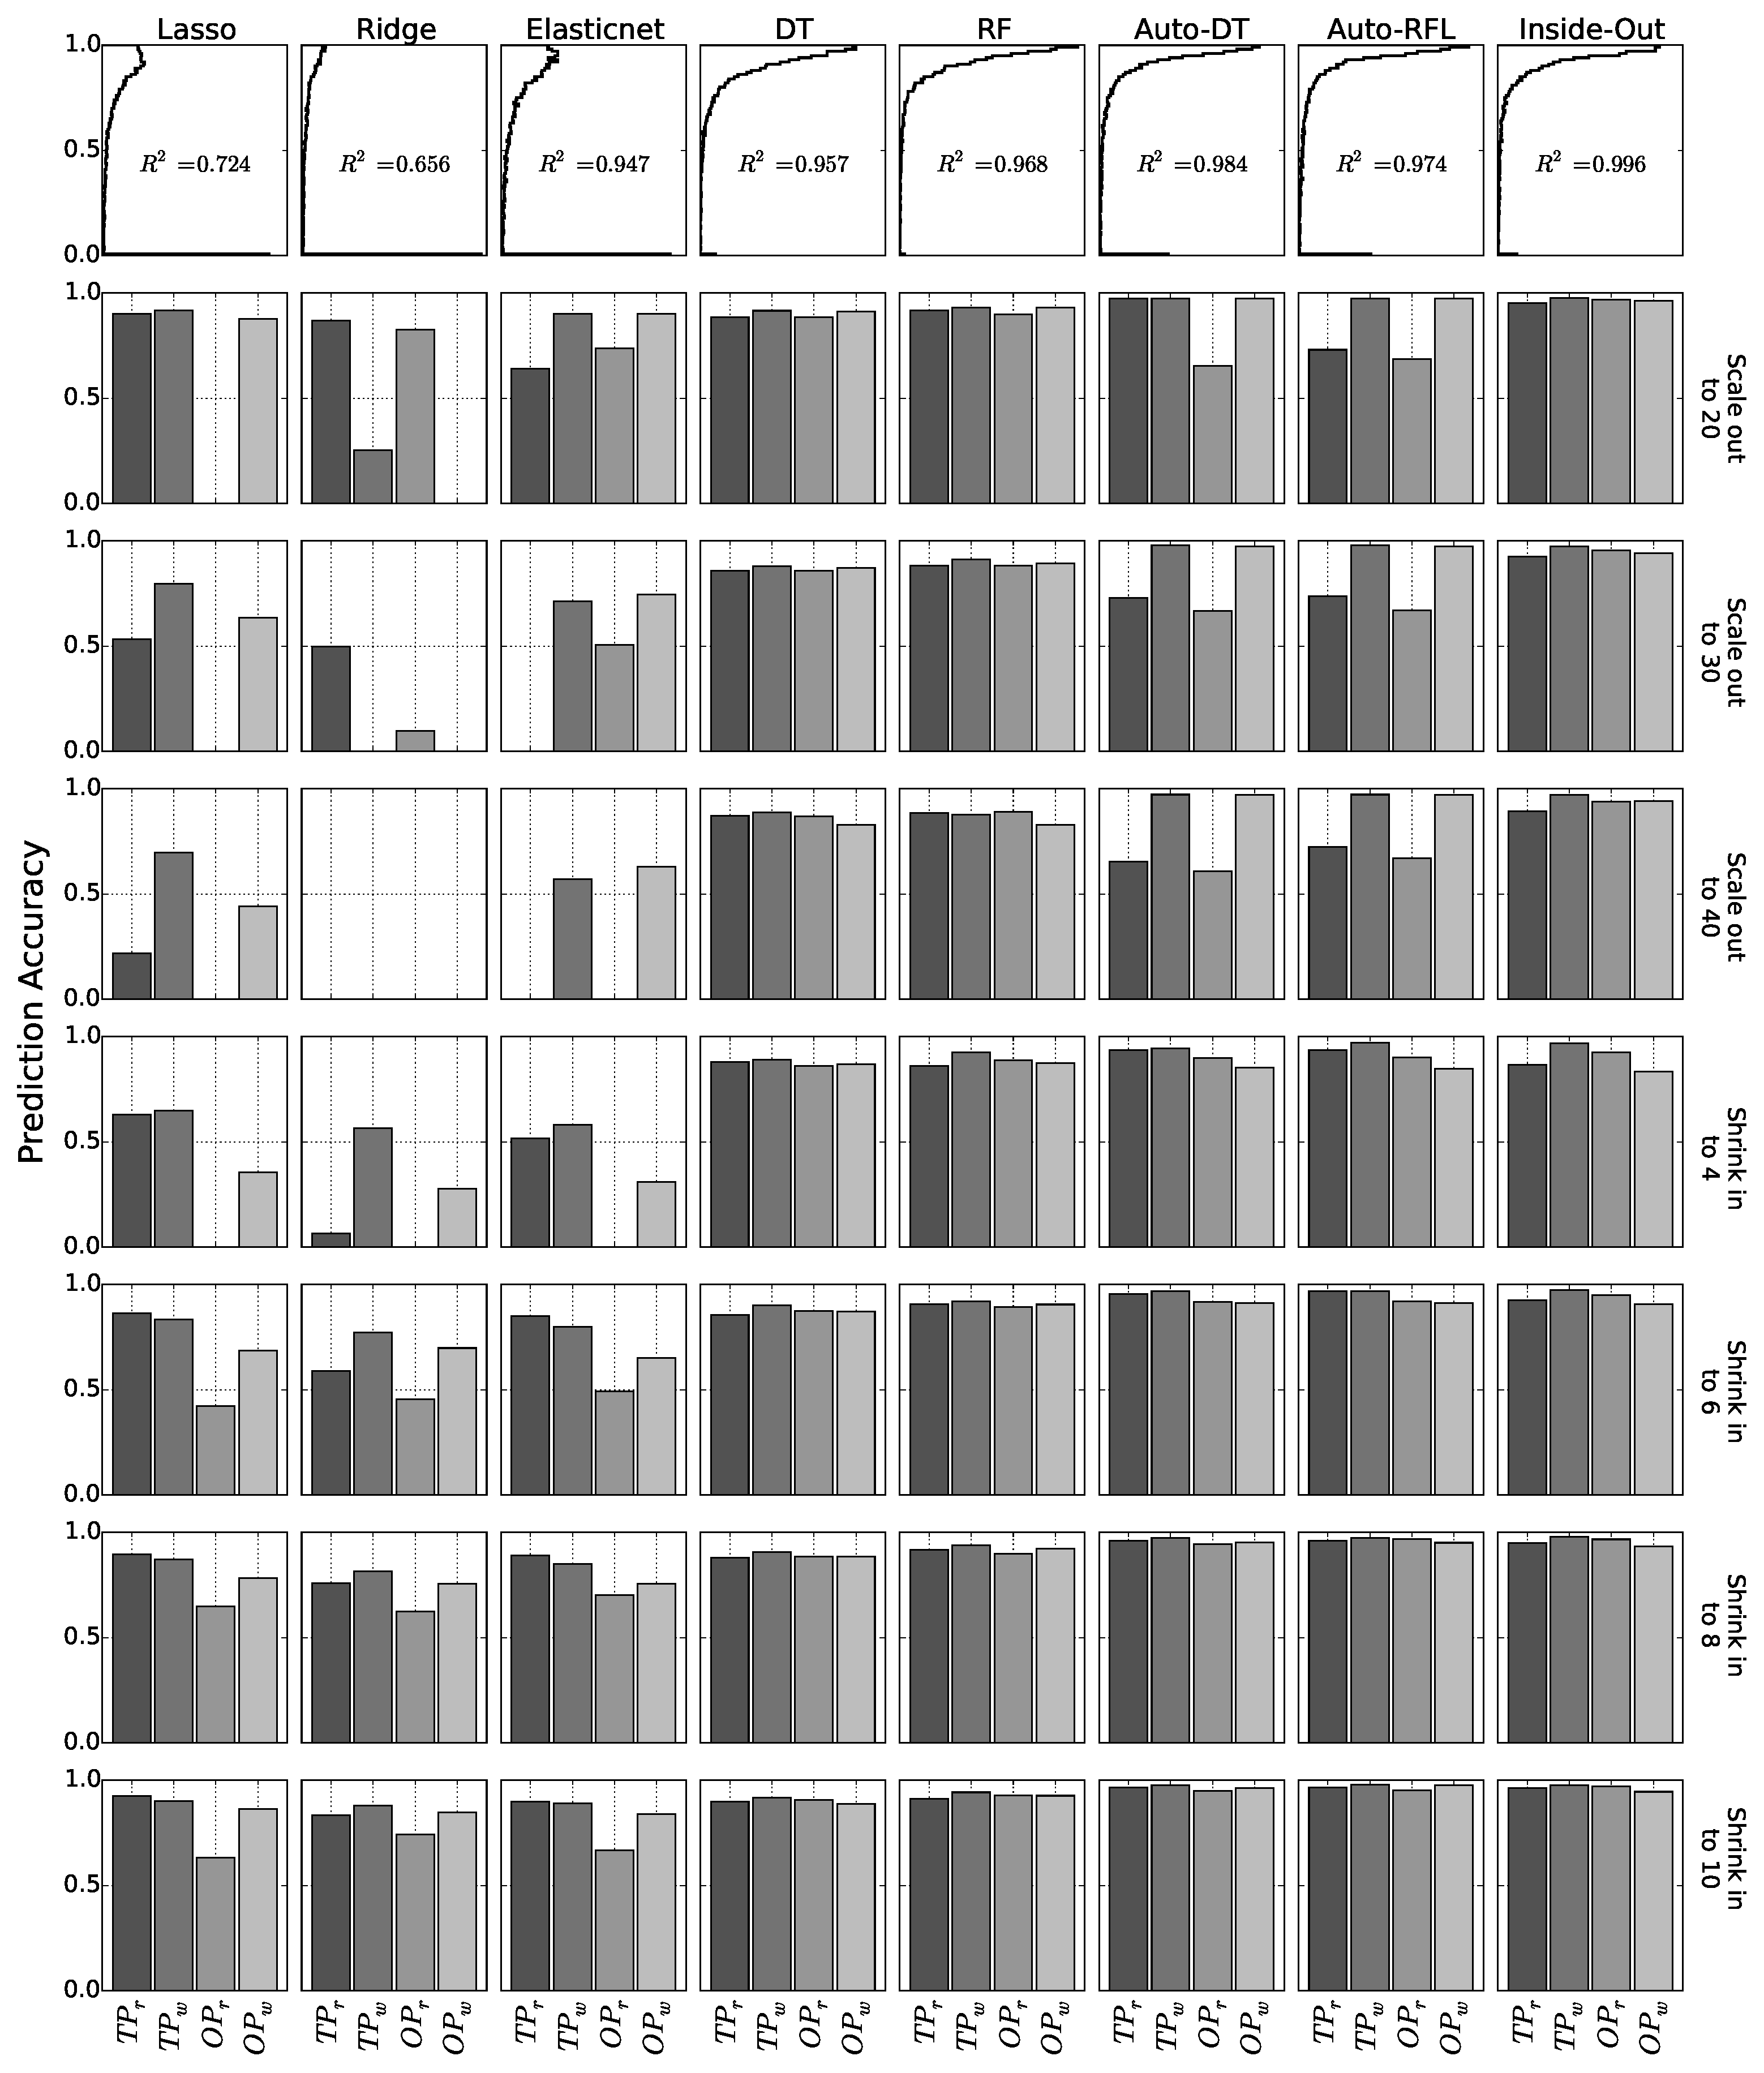
\includegraphics[width=0.9\textwidth]{Chapter-InsideOut/figures/unseen_scale_all_new.eps}
    \caption{Comparison of model performance in the on-demand scaling scenario. In the scale-out scenario, a performance model trained with 10 Ceph nodes is used to predict the performance of Ceph cluster with 20, 30 and 40 nodes.}
    \label{fig:elasticity}
\end{figure}


\subsection{Prediction Performance in a Multi-tenant Cloud}

This section examines the modeling performance of Inside-Out.
We first evaluate whether Inside-Out is able to extrapolate
performance of a larger Ceph cluster. 
Next, we evaluate how Inside-Out performs
when systems are subject to performance interference.

\subsubsection{Elastic Storage (On-demand Scaling)}
\label{sec:scaleout_prediction}

A storage service needs to grow or shrink its capacity on demand.
We evaluate Inside-Out's ability to capture the storage behavior at different system scales.
As shown in \myfigure{\ref{fig:elasticity}}, we use training data collected from 
4, 6, 8, and 10 nodes, and then predict the performance of 20, 30, and 40 nodes.
We also evaluate prediction accuracy in the \emph{shrink-in} scenario.
For both read and write throughput predictions, the linear models exhibit high variance.
In the $OP_r$ and $OP_w$ cases, the prediction results are not even comparable to the other methods.
Inside-Out, on the other hand, helps mitigate this issue, and achieves more than 90\% accuracy.
With increasing sizes of the storage, the prediction accuracy decreases because the prediction target 
becomes increasingly different from the training data.
Running a benchmark test against a very large system is time-consuming.
Here we demonstrate that Inside-Out can predict performance for systems that are 
four times larger than the system for which training data was collected.
%Due to resource limitations, we cannot show the upper bound of the largest system size that we can predict.
%However, we believe the upper bound can increase as the performance model keeps learning the system behavior.

\begin{figure}
    \centering
    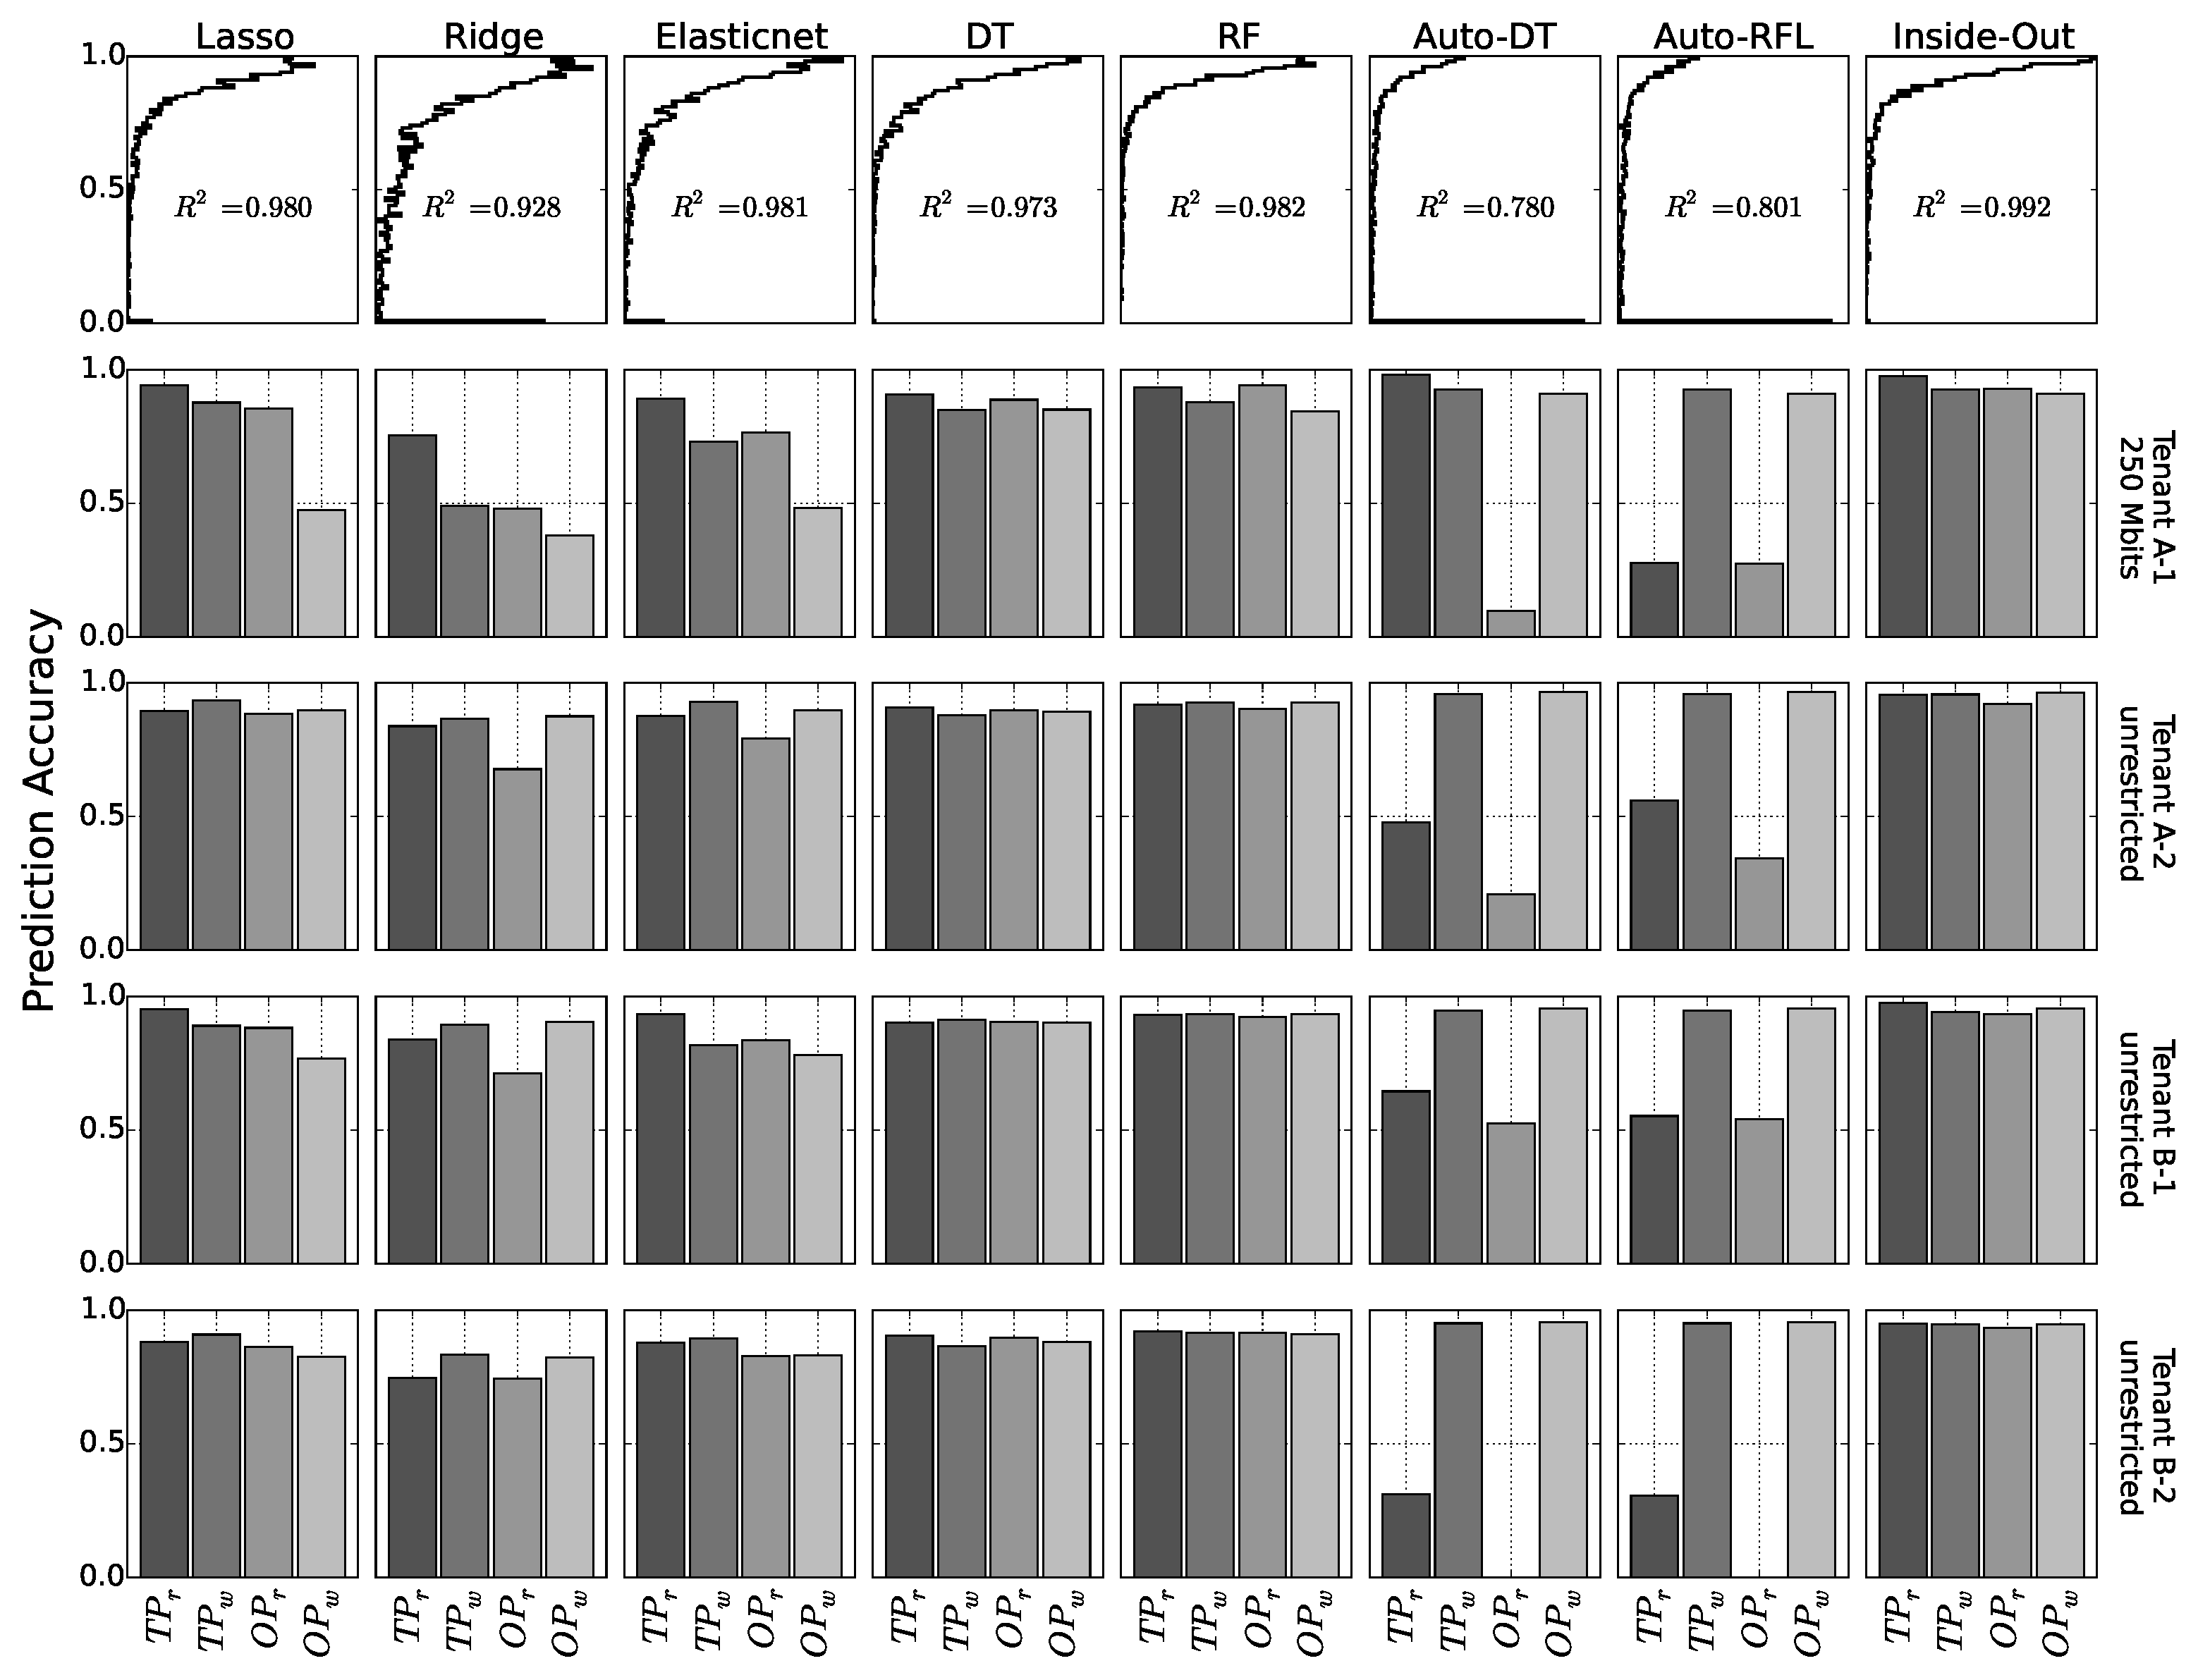
\includegraphics[width=0.9\textwidth]{Chapter-InsideOut/figures/multi_tenancy_all_new.eps}
    \caption{Prediction accuracy in a multi-tenancy scenario. Tenant A-1 is co-located with Tenant B-2. Tenant A-1 is throttled at 250Mbps. Tenant B-1 and B-2 are co-located without any traffic throttling.}
    \label{fig:multi_tenancy}
\end{figure}


\begin{figure*}
    \centering
    \includegraphics[width=0.9\textwidth]{Chapter-InsideOut/figures/real-world_tp_read.pdf}
    \caption{Application of Inside-Out to real time prediction of read throughput on a 10-node Ceph cluster.  Inside-Out starts from a simple prediction model trained by our collected benchmarking data.  Inside-Out keeps learning the storage behavior while improving prediction accuracy over time.}
    \label{fig:real_workload}
\end{figure*}


\subsubsection{Multi-Tenancy}
 
Next we evaluate Inside-Out's ability to adapt to performance interference among storage tenants.
We consider two cases for this evaluation. 
Each tenant runs a Ceph cluster with 10 OSDs separately, but tenants share the same 10 physical machines.
In the first case, we restrict the bandwidth of only the first tenant at 250Mbps.
%Two tenants compete for resources and \chin{\textbf{Tenant A-1}} has lower bandwidth SLO.
In the second case, we run two concurrent Ceph clusters but without network throttling.
\myfigure{\ref{fig:multi_tenancy}} shows that most prediction models are able to achieve more than 80\% accuracy.
The linear models like Ridge and Elasticnet yield lower prediction accuracies in some cases; however, Inside-Out performs well consistently.
Performance interference is challenging for a performance model designed for an isolated environment.
This evaluation demonstrates that the low-level performance metrics are good proxies for measuring
the end-to-end storage performance, even in a shared SDS environment.
%These metrics are able to reflect the behavior changes in the storage system.

%low-level performance feature selection approach is effective in capturing end-to-end performance, even under high storage interference.
%This property is important to SDS because it can help guarantee reliable end-to-end performance in a shared SDS environment.



\begin{comment}
\begin{figure*}
    \centering
    \includegraphics[width=0.9\textwidth]{figures/synthetic.eps}
    \caption{An online prediction scenario about six-hour long workload.  This synthetic workload is composed of 360 stages and each stage uniformly selects parameters such as workload types, request sizes and the number of clients.  The average stage duration is 60 seconds with standard deviation 20 seconds.}
\end{figure*}
\end{comment}

\begin{comment}
\begin{figure*}
    \centering
    \begin{subfigure}[b]{0.45\textwidth}
        \includegraphics[width=\textwidth]{figures/synthetic_read.eps}
        \caption{Read Throughput}
        \label{fig:synthetic_read}
    \end{subfigure}
    ~ %add desired spacing between images, e. g. ~, \quad, \qquad, \hfill etc.
      %(or a blank line to force the subfigure onto a new line)
    \begin{subfigure}[b]{0.45\textwidth}
        \includegraphics[width=\textwidth]{figures/synthetic_write.eps}
        \caption{Write Throughput}
        \label{fig:synthetic_write}
    \end{subfigure}
    \caption{An online prediction scenario about six-hour long workload.  This synthetic workload is composed of 360 stages and each stage uniformly selects parameters such as workload types, request sizes and the number of clients.  The average stage duration is 60 seconds with standard deviation 20 seconds.}
    \label{fig:synthetic_workload}
\end{figure*}
\end{comment}

%\subsection{Synthetic Workload}
\subsection{Online Self-Learning}
\label{sec:online_learning}

%Our goal is to apply Inside-Out to an online system so that SDS providers can guarantee the performance of a storage service hosted on their SDS platform.
%To evaluate this potential, 
Next, we create several synthetic workloads with mixed read/write ratios.
This synthetic workload spans 12 hours with 720 stages.
Each stage is 60-second long on average, with a standard deviation of 20 seconds.
We run four COSBench virtual machines for benchmarking and up to eight threads per COSBench client, with 10 Ceph OSDs and one monitor daemon.
We use Inside-Out to build an initial performance model with the training dataset described in Section~\ref{sec:dataset}.
\myfigure{\ref{fig:real_workload}} shows the prediction result for read throughput.
We can observe that the generated model can capture the overall trend, but suffers from over and under predictions.
This is because our training dataset is generated from a relatively clean environment, \ie the OS memory is flushed before any benchmarking process.
However, in the online prediction setting, cache is continuously consumed by non-stop client requests, which 
causes the real time storage behavior to be different from the training dataset.
With continuous monitoring of the performance of the storage service, 
we use Inside-Out to generate a new performance model at the sixth hour.
\myfigure{\ref{fig:real_workload}} shows that Inside-Out learns the new storage behavior and therefore, 
the over- and under-prediction issues are greatly mitigated.
%This evaluation demonstrates the potential of Inside-Out when applying it in an online system.
By continuously learning the storage behavior, SDS can accurately capture performance changes and therefore is able to provide reliable storage service.

%the problems due to over- and under-predictions are greatly mitigated.
%This evaluation demonstrates how Inside-Out can be used to continuously learn the storage behavior in an online system.


\begin{figure}
\centering
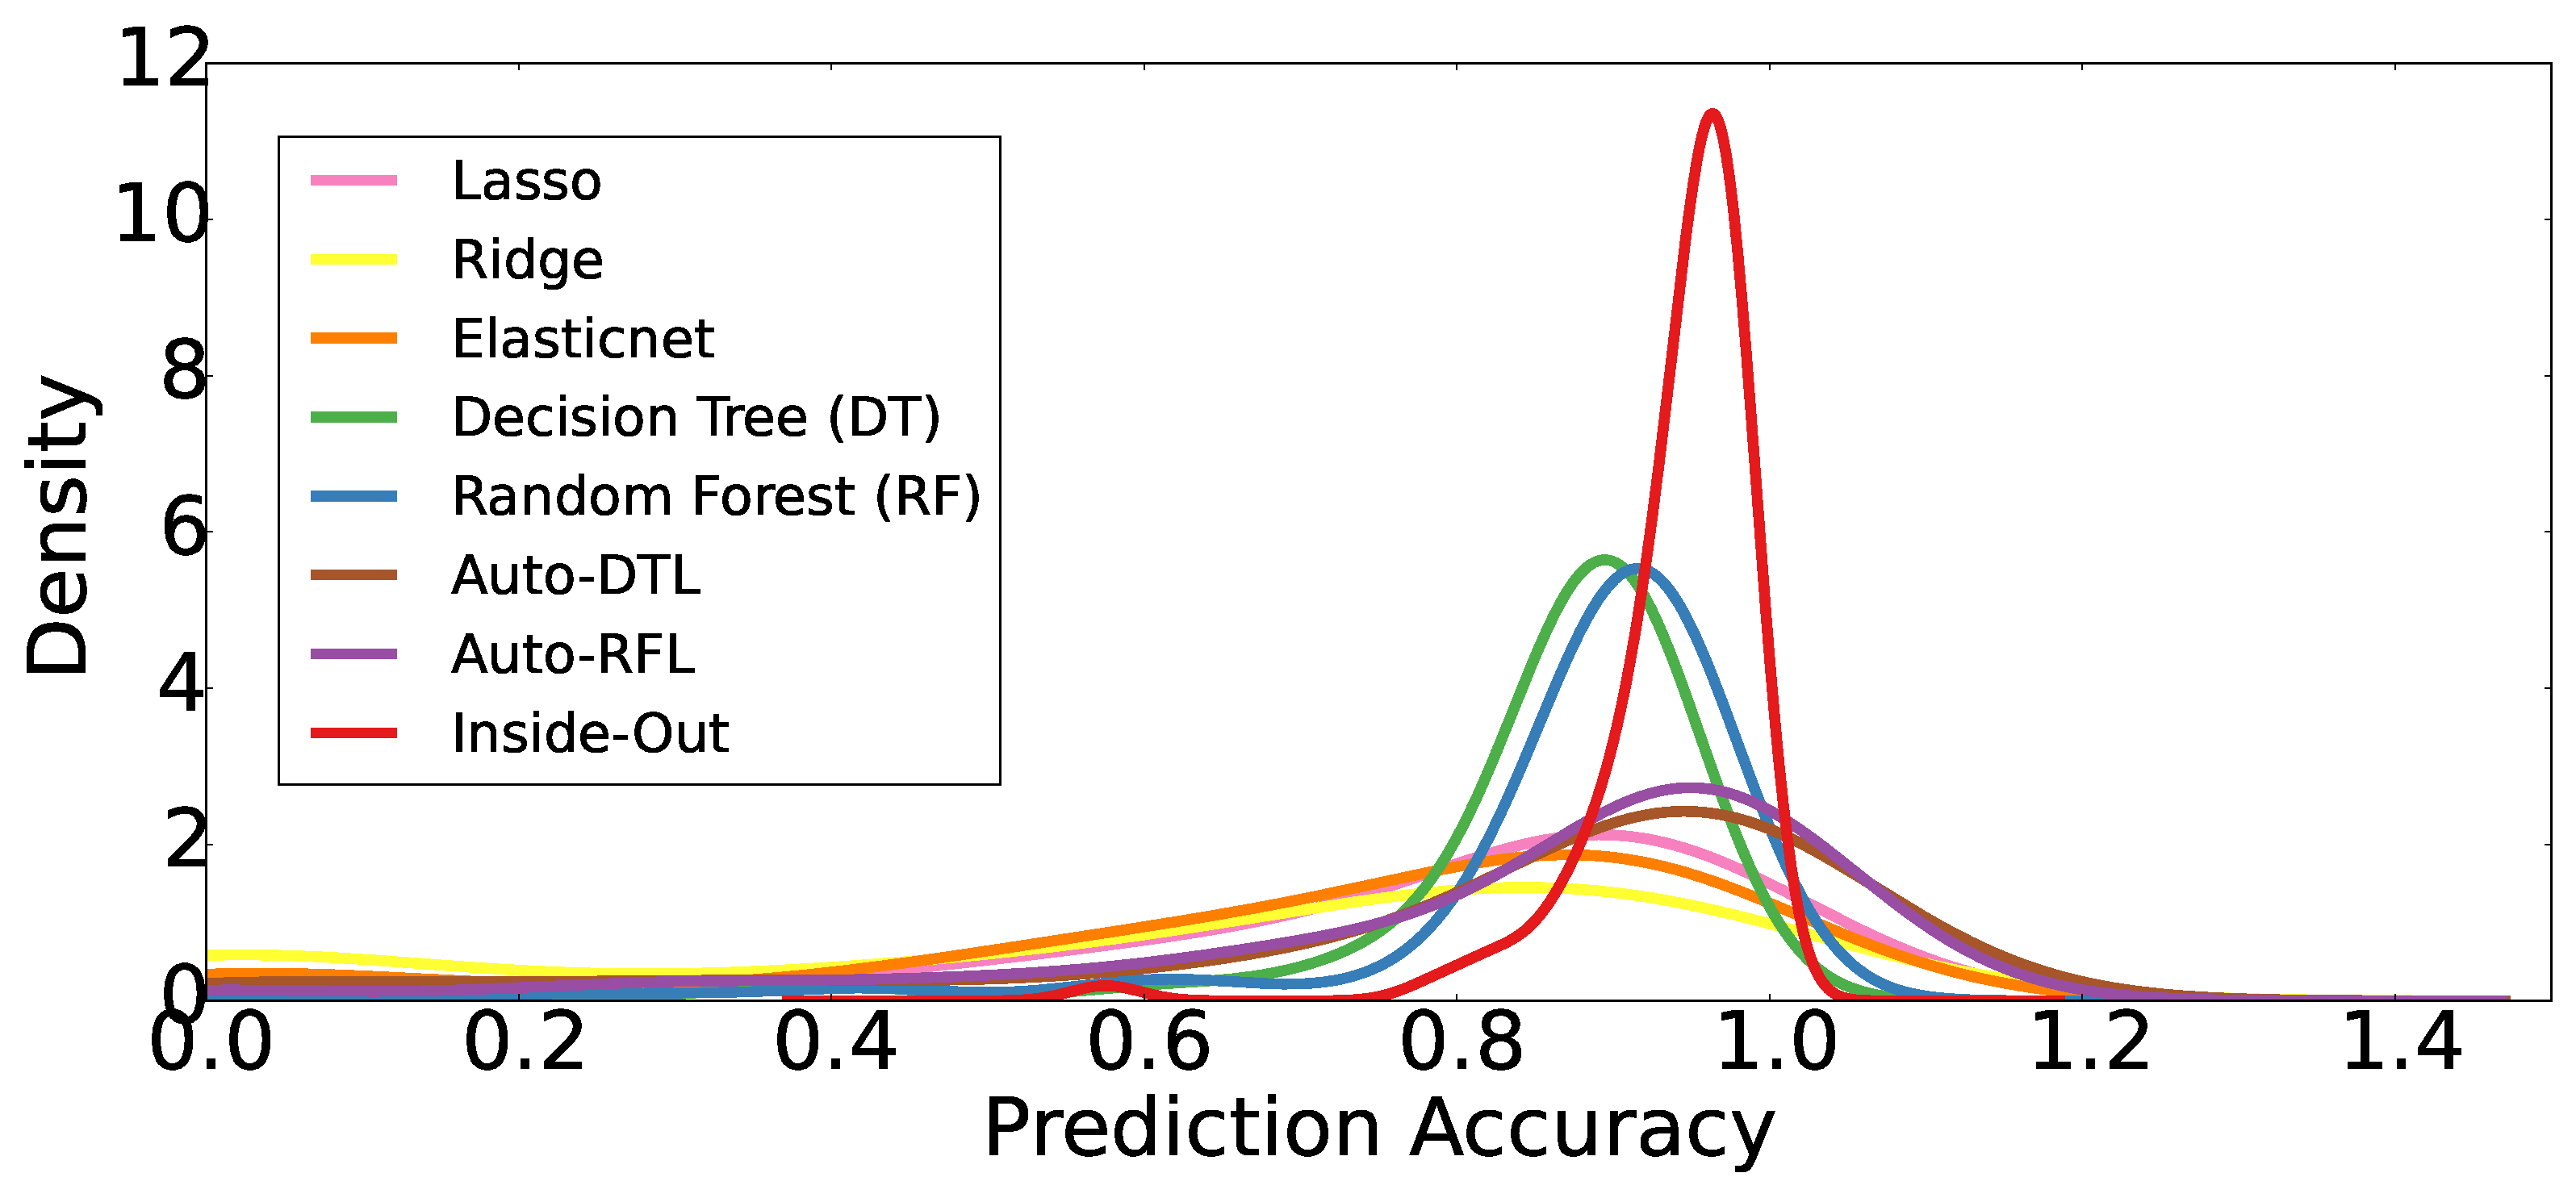
\includegraphics[width=0.9\textwidth, keepaspectratio]{Chapter-InsideOut/figures/aggregate_median.eps}
\caption{Kernel density function of prediction accuracy from \myfigure{\ref{fig:changing_workload}} to \myfigure{\ref{fig:multi_tenancy}}.  Each colored line represents the density function of a modeling approach.  Inside-Out is more consistent and accurate across almost every prediction case.}
\label{fig:aggregate}
\end{figure}


\vspace{1ex}
\subsection{Discussion}
We have shown that low-level performance metrics are useful to predict end-to-end throughput and IOPS.
%We applied Inside-Out to latency prediction and observe large variance and inconsistency.
%\chin{One} possible explanation is insufficient features and high variance in latency.
%The \chin{collected} low-level metrics are related to utilization, and these metrics might not provide enough information to fit a good model for predicting latency.
%Common approaches usually require request-level information \cite{Wang2004}.
%We need to further investigate latency prediction with other alternative generic low-level performance metrics.
Our evaluation has shown that low-level performance metrics are good indicators of end-to-end throughput and IOPS. 
Most existing performance models exhibit an inconsistent prediction behavior in the presence of diverse storage scenarios, 
such as changing workload, storage reconfigurations,
growing/shrinking storage, and multi-tenancy environments.
Our proposed two-level learning method can greatly improve prediction accuracy and yield consistent behavior.
Machine learning provides powerful tools, but they need to be used intelligently to achieve the best prediction accuracy. 
\myfigure{\ref{fig:aggregate}} shows the kernel density function of prediction accuracy across all prediction scenarios.
Inside-Out is a clear winner in terms of accuracy and consistency. 
More importantly, Inside-Out is able to learn new storage behavior, thereby enabling the performance model to adapt to the complex SDS environment.





% %\section{Related Work}
\label{sec:related_work}

\begin{itemize}
\item
  Characterizing application
\item
  Analyzing the energy-time trade-off in high-performance computing
  applications
\item
  Dynamically Controlling Node-Level Parallelism in Hadoop
\item
  Data-Driven Performance Modeling
\item
  Model Building

  \begin{itemize}
  \item
    Inside-out
  \end{itemize}
\item
  Configuration Recommendation
\item
  Parameter Tuning

  \begin{itemize}
  \item
    Selfish
  \item
    Dynamically Controlling Node-Level Parallelism in Hadoop
  \end{itemize}
\item
  Storage configurations
\item
  Cloud configurations

  \begin{itemize}
  \item
    Earnest
  \item
    CherryPick
  \end{itemize}
\item
  Search Algorithms
\item
  Random Search
\item
  Coordinate Descent
\item
  Genetic Algorithm
\item
  Bayesian Optimization
\end{itemize}
% \section{Conclusion}
\label{sec:conclusion}

The decoupled Hadoop model is flexible and much more preferable in many scenarios.
However, existing Hadoop schedulers do not consider this model and hence the scheduling method fails to optimize the system throughput.
Our flow scheduling method uses the penalty cost for task assignments in order to increase the processing flow rate on computing facilities.
We encode this problem as the min-cost flow problem and then we can obtain the optimal assignment.
We have implemented a pluggable Flow Scheduler for Hadoop YARN and it supports the latest version of Hadoop.
Our experiment results have shown that our flow scheduling can greatly improve the system throughput by about 30\% so as to eliminate stragglers.
These results support that the proposed flow scheduling can maintain the flow rate of processing.

Flow scheduling seems efficient for the decoupled model, but there still remains large space to improve.
For our current implementation, Flow Scheduler requires job profile and machine profile, which is not practical.
We believe we can estimate the flow demand of tasks and the flow capability of facilities at runtime.
A naive approach is to sample the flow demand of a task and then use this information to decide the cost of the remaining tasks of the same job.
Another approach is to monitor the flow rate of tasks so that we can adjust the penalty cost dynamically.
We can also decide the flow capability of facilities in a similar way.
Overall, we are positive about flow scheduling but more extensive evaluations have to be conducted before we can conclude.

% \chapter{A Collective CAT Optimizer for Multiple Workloads}
\label{chapter:micky}

This chapter proposes a collective optimization method
for a group of workloads in the CAT setting.

\section{Introduction}
\label{ch4:sec:introduction}

Many storage systems are moving away from dedicated appliance-based storage model to software-defined 
storage (SDS), which separates software that provisions and manages storage from the hardware that provides raw physical storage~\cite{sds_att, Thereska2013, Jalaparti2012}.
This trend is partly driven by the tremendous growth of data and the emergence of cloud applications that operate in a multi-tenant environment with diverse workload characteristics.
As a result, the rigid appliance-based model, with tightly-coupled hardware and software features, is no longer cost-effective, lacks flexibility, and does not scale well.
SDS systems are increasingly abandoning centralized storage services in favor of distributed systems like Ceph~\cite{ceph}, HDFS~\cite{hadoop}, Swift~\cite{openstack}. 
Distributed storage systems are attractive because they scale well, allowing storage services to grow or shrink, based on storage demands. 
They are also better suited to handle diverse multi-tenant workloads. 

Providing reliable quality of service (QoS) to storage applications is critical in an SDS environment shared by multiple applications 
with diverse usage patterns. However, in a distributed storage environment, it is challenging to provide storage QoS in a consistent 
and reliable manner. Practical deployments of modern distributed storage systems like Ceph are composed of a large number of 
individual storage components that can interact in a complex manner. 
Diverse and time-varying storage workloads and performance interference in a multi-tenant environment further 
complicate the reliable assurance of storage QoS. Reliable and accurate monitoring of 
high-level storage performance metrics (e.g. throughput and IOPS) is critical 
for providing storage QoS guarantees.    
However, monitoring end-to-end storage performance is difficult in a distributed storage service. 
Instrumenting user applications to measure storage performance is not always practical. 
Performing benchmark tests in production systems also has practical limitations since they 
interfere with storage application workload.
Furthermore, running exhaustive benchmark experiments to cover diverse application workloads, 
deployment topologies, and large configuration parameter space is time-consuming and impractical in many cases. 
Building accurate analytical performance models, on the other hand, is also difficult for the reasons mentioned above.
 
This chapter proposes the idea of using low-level system metrics (e.g., CPU usage, RAM usage and network I/O)
as a proxy for measuring high-level performance (e.g., end-to-end IOPS and throughput) of 
distributed storage applications.
We design, implement and evaluate a practical tool, called \emph{Inside-Out}, that applies 
machine learning techniques to the low-level metrics collected from individual components 
of a distributed storage system to accurately estimate high-level storage performance metrics---like throughput and IOPS---of the entire 
distributed storage system.
We believe that a tool like Inside-Out can serve as an important component of the overall SDS architecture.

Inside-Out takes a black-box modeling approach, which does not require knowledge about distributed storage system protocol, workload characteristics, and deployment topology. 
Inside-Out relies upon machine learning techniques to automatically derive an accurate end-to-end performance model.
We explore several well-known machine learning algorithms including linear regression, 
decision tree learning, and ensemble methods \cite{Wang2004, Noorshams2013}, and conclude that  
there does not exist an one-size-fits-all algorithm that can work in all prediction cases.
Hyperparameter tuning \cite{Chapelle2002, Noorshams2013}, model selection \cite{Kohavi1995} and 
feature selection \cite{guyon2003introduction, Saeys12007} all turn out to be too complicated for optimizing prediction accuracy.
In contrast, Inside-Out uses a two-level learning method that automatically selects important features, boosts prediction accuracy, and achieves consistent prediction. 
This two-level learning method pipelines two supervised learning algorithms to eliminate irrelevant features while avoiding overfitting problems.\footnote{\label{ft:overfitting}
Overfitting describes the situation when a model captures the relationship of noisy data but not the underlying relationship \cite{domingos2012few}.
Overfitting becomes more prominent in the presence of high dimensional data}

Inside-Out offers several key benefits. 
%[MRA] Unlike traditional analytic performance modeling approach, Inside-Out is generic in nature, and therefore, it can be applied to different storage services.  
Unlike traditional analytic performance modeling approach, Inside-Out is more generic, 
and therefore can be more easily applied to different storage services.  
Different from previous work, Inside-Out 
does not require information about system configuration and application workload~\cite{Ruemmler1994, Shriver1998, Wang2004, Kelly2004, Yin2006, Noorshams2013, Ardagna2014}. 
Due to the self-learning property, \emph{Inside-Out} improves performance prediction accuracy with more data.
It can also adapt to changes in the system
by continuously learning the system behavior. 

We evaluate Inside-Out using Ceph~\cite{ceph} %as an example distributed storage system 
running on an OpenStack-based SDS platform.
The low-level performance metrics are collected from participant virtual machines 
running various components of a Ceph storage service.\footnote{\label{ft:vm}
Our approach is not limited to VM-based environments.
It can be applied to container-based and bare-metal storage servers as well.
}
Our in-depth evaluation shows that Inside-Out generates end-to-end performance models with 91.1\% prediction accuracy on average.
More importantly, as discussed above, Inside-Out is generic in nature as it captures the behavior of the storage system 
by analyzing low-level system metrics (that are protocol and application agnostic). Furthermore, we demonstrate that Inside-Out 
%[MRA] can provide reliable performance monitoring even in the presence of evolving workload characteristics, changing storage 
can provide reliable hints for performance monitoring tasks even in the presence of evolving workload characteristics, changing storage 
configuration and interfering tenants. We also show that Inside-Out is reliable in estimating end-to-end performance 
even when the storage system expands or shrinks.
We show that Inside-Out provides reliable performance 
prediction when the storage system is up to four times larger than the one used for building machine learning models during 
the training phase. 
Lastly, Inside-Out is able to learn new storage behavior over time.
\section{Why Collective Optimization}
\label{sec:motivation}

A cloud optimizer is often evaluated with search performance and measurement cost.

\begin{itemize}
\item \textbf{Search performance} is the measure of the quality of the found solutions by an optimizer.
For example, in searching for the most cost-effective configuration, an optimizer that finds a configuration that is only 10\% more expensive than the optimal is considered better than another optimizer
that can only find a configuration that yields 30\% more cost.
Therefore, we use normalized performance (to the optimal) for evaluation.

\item \textbf{Search cost}
is the total cost of running an optimizer.
An optimization process is expensive because it requires
to test a workload on some cloud configurations for deriving
the best choice.
We use the number of tests as the search cost (or measurement cost)
because it is an intuitive measure.
The amount of charge is another measure~\cite{Alipourfard2017}. 

\end{itemize}


There is always a trade-off between measurement cost and search performance.
The primary motivation for collective optimization is to reduce high measurement cost of optimizing multiple workloads.
If users demand strict search performance, they better turn to single-optimizers.
However, we argue that collective optimization is promising
because it achieves comparable or slightly worse search performance
while reducing measurement cost significantly.
In the following,
we discuss the benefits of having a collective optimizer.


\begin{itemize}
\item \textbf{Large scale cloud migration.}
Cloud computing is a cost-effective solution.
Enterprises are moving in-house applications to the cloud,
and need a quick way for large migration~\cite{khajeh2010cloud,sripanidkulchai2010clouds}.
Elaborate optimizers are expensive (in measurement cost) and time-consuming (in optimization process).

\item \textbf{Limited budgets.}
The single-optimizer such as \emph{CherryPick} and \emph{Scout} are effective and desirable for highly recurring workloads because the measurement cost can be amortized.
However, the number of budgets to run optimizers
does not increase linearly with the number of workloads.
To better support multiple workloads,
we need to reduce measurement cost while delivering comparable search performance.

\item \textbf{Expanding cloud portfolio.}
Cloud providers expand their cloud portfolio more than 20 times in a year~\cite{ec2history}.
Therefore, users have to rerun optimizers to update their configurations for all workloads.
Again, this is an expensive and time-consuming process.

\item \textbf{Seed cloud optimizers.}
All the cloud optimizers require initial measurements.
It is unclear how to determine the best starting points.
We aim to find the exemplar configurations,
which can be used as the starting points, thereby
reducing measurement cost.
The exemplar configuration can be used to seed singe-optimizers such as CherryPick and \scout, which will be discussed more in Section~\ref{sec:system}.

\end{itemize}

In summary, users would prefer collective optimization if search performance is comparable to single-optimizers while measurement cost can be reduced greatly.

\begin{figure}[!htbp]
\centering
\begin{subfigure}[b]{0.5\textwidth}
    \includegraphics[width=\linewidth]{Figures/motivation_cost_hadoop_percentage.pdf}
    \caption{Hadoop 2.7}
    \label{fig:motivation_percentage_1}
\end{subfigure}
\begin{subfigure}[b]{0.5\textwidth}
    \includegraphics[width=\linewidth]{Figures/motivation_cost_spark_percentage.pdf}
    \caption{Spark 2.1}
    \label{fig:motivation_percentage_2}
\end{subfigure}
\begin{subfigure}[b]{0.5\textwidth}
    \includegraphics[width=\linewidth]{Figures/motivation_cost_spark1.5_percentage.pdf}
    \caption{Spark 1.5}
    \label{fig:motivation_percentage_3}
\end{subfigure}
\caption{\textbf{Opportunity to find the exemplar VM instances across workloads for reducing operational cost.} The \emph{y-axis} represents the percentage of workloads (out of 107 in three systems) that are within 30\% difference with the optimal performance.  The colored bars are VM types that considered the exemplar configurations for the majority of workloads ($>= 50\%$).
 The \textcolor{red}{red} bar represents that the VM type is more likely to be the optimal choice.}
\label{fig:motivation_percentage}
\end{figure}


\section{Finding the Exemplar Cloud Configuration}
\label{sec:mab}

In this section, we first present our empirical study
on investigating the potential of finding the exemplar cloud configuration.
We then formulate ``finding the exemplar configuration in the cloud'' as the multi-armed bandit problem.
Finally, we discuss the heuristics to derive the exemplar configuration.

%\todo{we can extend to find multiple exemplar configurations}


\subsection{Empirical Study}
\label{sec:empirical}

We choose three popular software systems for cloud applications, namely Apache Hadoop 2.7, Spark 2.1 and Spark 1.5.
This study includes 30 applications for diversification.
They are data processing, OLAP queries, common statistics functions, and
popular machine learning algorithms.
Although they do not cover all the spectrum of real-world applications,
they are representative of many nowadays cloud applications.
When the input to applications changes, the workload behavior changes accordingly~\cite{Venkataraman2016, Dalibard2017}.
We also choose three different input parameters and data sizes for each application.
In total, our evaluation includes 107 workloads.

We conduct our evaluation on AWS EC2~\cite{aws}.
Regarding the VM to run the workloads, we choose 18 different VM types.
They include three instance families:
1) compute-optimized instances (\emph{c3} and \emph{c4}),
2) memory-optimized instances (\emph{r3} and \emph{r4}), and
3) general-purpose instances (\emph{m3} and \emph{m4}).
For each instance family, we choose \emph{large}, \emph{xlarge} and \emph{2xlarge} for the instance size.
Although we only evaluate 21\% VM types (AWS supports 85 kinds as of January in 2018),
they reflect many use cases on AWS EC2.
Besides, some VM types are designed for acceleration using GPU and FPGA, and therefore, they are less common and not included.
Furthermore, it is reported that VM types with lower than 8 cores dominate VM useage on Azure~\cite{Cortez2017}.
We try our best to reflect the common cloud deployment.
More details regrading data collection can be found in our previous work~\cite{Hsu2018Arrow, Hsu2018Scout}.
We also made our data public available for further research~\cite{scoutdataset}.
Please refer Section~\ref{sec:cat::dataset} in more detail.



\subsection{The Exemplar Configurations}
\label{sec:exemplar}
The exemplar configurations are configurations that
are near-optimal or satisfactory in the majority of workloads.
When the percentage is large, 
we can exploit the exemplar configurations to simplify collective optimization.
In \myfigure{\ref{fig:motivation_percentage}}, we present the opportunity of exploiting such configurations.
We count the number of the normalized performance that is within 30\% of the optimal.
The colored bars are possible exemplars because they are satisfactory at least in half of the workloads.
The red bar represents the VM type that is more likely to be the optimal than other configurations.
These figures show there exist several exemplar configurations.


% datasize=medium
\begin{table}[!htbp]
\centering
\caption{\textbf{Normalized performance on a selected group of VM types and workloads.}  The number $1.0$ represents the optimal choice across the 18 VM types for the particular workload.}
\label{table:dataset}
%{\scriptsize
\resizebox{0.75\columnwidth}{!}{%
\renewcommand{\baselinestretch}{0.5} 
\begin{tabular}{@{}c@{~}l@{~}r@{~}r@{~}r@{~}r@{~}r@{}}
\toprule
\multicolumn{1}{l}{\textbf{System}} & \textbf{Workload} & \textbf{c3.large} & \textbf{c4.large} & \textbf{c4.xlarge} & \textbf{m4.large} & \textbf{m4.xlarge} \\ \midrule
\multirow{6}{*}{\rotatebox[origin=c]{90}{\parbox[c]{1.5cm}{\centering Hadoop 2.7}}} & aggregation & 1.26 & 1.00 & 1.12 & 1.12 & 1.29 \\
 & join & 1.26 & 1.00 & 1.09 & 1.17 & 1.26 \\
 & scan & 1.16 & 1.00 & 1.70 & 1.15 & 1.89 \\
 & sort & 1.10 & 1.00 & 1.06 & 1.03 & 1.11 \\
 & terasort & 1.31 & 1.00 & 1.16 & 1.07 & 1.12 \\
 & pagerank & 1.24 & 1.03 & 1.16 & 1.05 & 1.00 \\ \midrule
\multirow{10}{*}{\rotatebox[origin=c]{90}{\parbox[c]{1cm}{\centering Spark 2.2}}} & join & 1.12 & 1.00 & 1.40 & 1.12 & 1.23 \\
 & scan & 1.13 & 1.00 & 1.48 & 1.03 & 1.59 \\
 & sort & 1.11 & 1.00 & 1.42 & 1.13 & 1.40 \\
 & terasort & 1.30 & 1.19 & 1.66 & 1.34 & 1.46 \\
 & wordcount & 1.83 & 1.64 & 1.23 & 1.00 & 1.08 \\
 & als & 1.00 & 1.67 & 3.19 & 1.46 & 2.72 \\
 & aggregation & 1.30 & 2.00 & 1.08 & 1.00 & 1.18 \\
 & pagerank & 2.33 & 2.12 & 1.00 & 1.31 & 2.10 \\
 & bayes & 3.15 & 3.57 & 1.00 & 1.60 & 1.61 \\
 & lr & 6.50 & 5.56 & 1.44 & 1.00 & 2.61 \\ \midrule
\multirow{19}{*}{\rotatebox[origin=c]{90}{\parbox[c]{1cm}{\centering Spark 1.5}}} & chi-feature & 1.19 & 1.00 & 1.32 & 1.29 & 1.53 \\
 & fp-growth & 1.27 & 1.00 & 1.37 & 1.20 & 1.46 \\
 & gmm & 1.19 & 1.00 & 1.27 & 1.25 & 1.36 \\
 & gb-tree & 1.19 & 1.00 & 1.63 & 1.17 & 1.94 \\
 & pca & 1.16 & 1.00 & 1.11 & 1.15 & 1.31 \\
 & pearson & 1.19 & 1.00 & 1.11 & 1.19 & 1.11 \\
 & word2vec & 1.22 & 1.00 & 1.06 & 1.15 & 1.24 \\
 & spearman & 1.21 & 1.00 & 1.12 & 1.06 & 1.02 \\
 & statistics & 1.15 & 1.00 & 1.43 & 1.08 & 1.56 \\
 & svd & 1.16 & 1.00 & 1.02 & 1.07 & 1.09 \\
 & chi-gof & 1.24 & 1.12 & 1.46 & 1.00 & 1.81 \\
 & bayes & 1.27 & 1.15 & 1.19 & 1.25 & 1.35 \\
 & lda & 1.66 & 1.36 & 1.10 & 1.00 & 1.31 \\
 & pic & 1.53 & 1.39 & 1.00 & 1.15 & 1.31 \\
 & d-tree & 1.70 & 1.70 & 1.23 & 1.00 & 1.48 \\
 & als & 2.23 & 1.86 & 2.89 & 1.00 & 1.27 \\
 & regression & 4.03 & 3.60 & 4.06 & 4.42 & 4.70 \\
 & classification & 6.11 & 5.41 & 5.70 & 6.07 & 1.00 \\
 & kmeans & 6.22 & 5.74 & 3.66 & 3.73 & 1.00 \\ \midrule
\multicolumn{2}{c}{\textbf{\# of optimal}} & 1 & 18 & 3 & 7 & 3 \\
\multicolumn{2}{c}{\textbf{Mean}} & 1.89 & 1.72 & 1.63 & \textbf{1.45} & 1.53 \\
\multicolumn{2}{c}{\textbf{25\%}} & 1.18 & 1.00 & 1.11 & 1.04 & 1.15 \\
\multicolumn{2}{c}{\textbf{Median}} & 1.26 & 1.00 & 1.23 & 1.15 & 1.31 \\
\multicolumn{2}{c}{\textbf{75\%}} & 1.68 & 1.69 & 1.47 & \textbf{1.25} & 1.58 \\ \bottomrule
\end{tabular}
}
\end{table}


In \mytable{\ref{table:dataset}}, we give snippets of measurement data to better illustrate the exemplar configurations.
This table presents the normalized performance of workloads on some of the VM types.
A $1.0$ number indicates the VM type is the optimal choice for the corresponding workload while a larger number implies a sub-optimal choice.
We can observe that \emph{c4.large} is the optimal configuration for 18 workloads (out of 35).
However, it is also a sub-optimal VM type ($>1.4$) in 11 workloads, which generating
$1.72$ normalized performance on average.
On the other hand, \emph{m4.large} seems to be a better choice because it delivers $1.45$ performance on average and creates only 5 sub-optimal workloads.
The above gives one way to select the exemplar configuration and in the following,
we describe the challenges of selecting the exemplar.



\begin{itemize}
\item \textbf{Varying workloads.}
In \mytable{\ref{table:dataset}}, we show five possible exemplar configurations for those particular workloads.
The exemplars very in different sets of workloads.
For example, \emph{c4.large} is the best choice in Hadoop 2.7 while
\emph{m4.large} should be selected as the exemplar VM type in Spark 2.1.

\item \textbf{Expanding cloud portfolio.}
As mentioned before, cloud providers introduce new VM types regularly, which
includes performance boost and price adjustment.
The exemplar configurations might also change accordingly.

\item \textbf{Online discovery.}
We present an offline analysis of measurement data above.
However, finding the exemplar configuration is an online task (for unknown workloads), which is considered a difficult learning problem.
This is similar to the exploration-exploitation dilemma~\cite{kaelbling1996reinforcement}.

\end{itemize}

From the above, it would appear that there exist exemplar configurations in real-world workloads.
Note that if the exemplar configuration is prevalent, it should be possible to simplify collective optimization as follows:
finding the exemplar configuration instead of finding the optimal choice for each of the workload.
The exemplar configurations deliver near-optimal to satisfactory performance in the majority of workloads.
The rest of this work is a test of that speculation.






\subsection{Problem Formulation}
\label{sec:formulation}

\micky attempts to find the exemplar VM type ($vm^*\in VM$) for a group of workloads ($W$).
The workload refers to a combination of an application and the data used.
The performance is measured in terms of \textit{execution time} and \textit{operational cost}. The cloud configuration space for workload
$w$ is referred to as ($s\in S_w$), where $S_w$ is the set of cloud configuration options for a workload $w$. The size
of the search space is $N_w$ cloud configurations. In our setting, the size of the cloud configuration space is same for all workloads. For a given workload $w$, each configuration $s$ has a corresponding performance
measure $y_{w, s} = \phi(w, s)$.
%Each configuration in the cloud configuration space $s$ is represented as the features of the cloud configuration such as number of cores, size of the memory.
%The objective is to find a cloud

Single-optimizers such as Cherrypick~\cite{Alipourfard2017} searches a suitable VM type for every workload $w$ separately.
The search starts with a pool of unevaluated configuration ($U_w$)---the specific workload has not been run on any configuration.
As the search proceeds, the cloud configuration are selected from $U_w$ and moved to the evaluated pool ($E_w$). The sum of the cardinalities
of $U_w$ and $E_w$ is equal to the cardinality of $S_w$ ($|U_w| +|E_w| = |S_w|$).
The measurement cost of the search process is $C_w=|E_w|$.
When optimizing a group of workloads,
single-optimizers generate a total cost $C=\sum_{w \in W} |C_w|$.

\micky is a collective optimization method.
We explore the exemplar VM type $vm^*$ so that 
$|E_{w_1} \cup E_{w_2} \cup \cdots \cup E_{w_n}|$ is minimized while the corresponding performance measure
$y_{w, vm^*}$ is comparable to the the ones in single-optimizers.



\subsection{The Multi-Armed Bandit Problem}

To realize collective optimization, we reformulate the problem of configuration optimization as a multi-armed bandit problem~
\cite{robbins1985some,weber1992gittins,bergemann2006bandit,audibert2011introduction}.
In the problem setting,
an agent  (gambler) sequentially searches for a slot machine (from a group of slot machines) to maximize the total reward collected in the long run. This problem is non-trivial since the agent (gambler) cannot access the true probability of winning---all learning is carried out via the means of trial-and-error and value estimation. To find the suitable slot machine, the agent needs to acquire information about arms  (exploration)  while  simultaneously  optimizing  immediate rewards  (exploitation).
The is referred to as the exploration-exploitation dilemma~\cite{kaelbling1996reinforcement}.
Finding the better VM type for workloads naturally fits into the multi-armed bandit problem.
We describe their similarities in the following.

\begin{itemize}
\item \textbf{Slot Machine.} Each VM type is similar to a slot machine. Our objective is to find the best VM that maximizes the reward for a group of workloads.
\item \textbf{Arm.} Arms are the choices of slot machines. In the cloud setting, an optimizer chooses a VM type to run a workload.
\item \textbf{Pull.} A pull is one play on the slot machine. It takes coins (cost) and yields a reward.
Similarly, an optimizer picks a VM type and measures the performance of a workload on the selected VM.
\item \textbf{Reward.} Reward refers to the amount of money a gambler wins or loses from pulling the arms.
In our setting, the reward is determined by where it meets a performance objective.
We use performance delta (between the selected and the optimal choice) for calculating the reward.
Please note that the optimal configuration is not known in the real-world setting.
\item \textbf{Budget.}
A gambler owns a certain amount to spend on the slot machines.
In our setting, an optimizer requires to complete the optimization process in a limited budget.
We use the number of measurements as the budget ($C$).
In practice, the minimal budget is usually $|\mathit{VM}|$
and the maximum budget is $|\mathit{VM}| \times |\mathit{W}|$.
The budget is determined by users.
A higher budget yields a better reward.
\item \textbf{Objective.}
The objective of \micky is to find the best configuration (minimize performance delta) for multiple workloads with fewer measurements.
\end{itemize}

The multi-armed bandit problems have attracted attention for solving online learning problems.
For example, 
Dambreville et al.~\cite{dambreville2017load} used multi-arm bandit to minimize the energy consumption of a cloud platform by
using workload prediction to reallocate the set of available servers.
Jiang et al. perform data-driven QoE (quality of experience) optimization for real-time exploration and exploitation~\cite{jiang2017pytheas}.
While we borrow techniques from this rich literature~\cite{bergemann2006bandit}, our contribution is to shed light on how to use these techniques to find the exemplar cloud configurations and to show collective optimization can solve the problem using only a fraction of measurement cost required by prior work.


\begin{figure}[!htbp]
\centering
\begin{subfigure}[b]{0.6\textwidth}
    \includegraphics[width=\linewidth]{Figures/s2_single_hadoop_cost_performance.pdf}
    \caption{Hadoop 2.7}
    \label{fig:single_time_steps}
\end{subfigure}
\begin{subfigure}[b]{0.6\textwidth}
    \includegraphics[width=\linewidth]{Figures/s2_single_spark_cost_performance.pdf}
    \caption{Spark 2.1}
    \label{fig:single_time_performance}
\end{subfigure}
\begin{subfigure}[b]{0.6\textwidth}
    \includegraphics[width=\linewidth]{Figures/s2_single_spark15_cost_performance.pdf}
    \caption{Spark 1.5}
    \label{fig:single_time_performance}
\end{subfigure}
\caption{\small{\textbf{Search performance of optimization methods in search for cost-effective cloud configurations.} Three software systems are evaluated.  \emph{CherryPick} finds good solutions in the three systems while \micky is comparable in Hadoop 2.7 but shows higher variance (sub-optimal choices).  We propose a integrated system (in \myfigure{\ref{fig:system_design}}) to detect those sub-optimal cases for improving \micky.}}
\label{fig:s2_cost_performance}
\end{figure}


\subsection{Heuristics}
\label{sec:methods}

% need to put softmax in the following text
% we might need to try thompson sampling
% need citation
In the literature, several strategies have been proposed to find the most rewarding slot machines (the exemplar configurations) in the multi-arm bandit setting.
These strategies can be divided into three major groups.
First, the \textit{Epsilon-greedy}, works by oscillating between (a) exploiting the best option which is currently known, and (b) exploring at random among all of the options available to it.
Second, the probability matching strategy selects the arms according to the probability of the arm being the optimal choice.
Thompson sampling or Bayesian Bandits are well-known probability matching strategies.
Last, in the contextual bandit problem, strategies such as Upper Confidence Bound (UCB) builds a predictor from existing observation for making a better decision.
UCB always opportunistically chooses the arm that has the highest upper confidence bound of reward, and therefore, it will naturally tend to use arms with high
expected rewards or high uncertainty.
The above only discusses some important methods.
It is not the major focus to design the best method but to evaluate the existing methods best for collective optimization.
\section{Evaluation}
\label{sec:evaluation}

This section presents our evaluation.
We introduce our experimental setup and benchmark
design.
We then evaluate different placement schemes
by measuring query throughput and
testing their robustness to slight workload mispredictions.


\subsection{Experiment Setup}

We conducted our evaluation on Virtual Computing Lab (VCL), a cloud
platform provided by NC State University.
All servers are equipped with 2-core Intel Xeon CPU and 8GB memory
and connected to a 10 Gbit switch. 
VCL only provides limited storage capacity of local disks or
\emph{instance storage}.
This is also the case for many cloud configurations.
In fact, a majority of EC2 instance types in Amazon Web Services (AWS) do not
have any instance storage.
Instead one must mount a remote volume served by a enterprise-level
storage system.
(AWS calls this \emph{elastic block storage}--EBS.)
We evaluate our approach using both instance storage (local disks) and
remote volumes provided by network file system (NFS),
backed by NetApp 2554 filer with dual controllers.

We evaluate our placement schemes on
high performance computing cluster (HPCC)~\cite{middleton2011hpcc}.
HPCC is an open source
data analytics computer developed by LexisNexis Risk
Solutions for processing big data.
They maintain several clusters with more than 100 nodes, the largest
with more than 500, to provide services to their clients.
Experiments were conducted on a HPCC Roxie cluster.
Roxie is a \emph{data delivery engine} that responds to queries.
It finds the answers to requests in an index that is partitioned and,
if desired, replicated across the nodes.
Roxie is optimized to handle massive amounts of concurrent requests
with low latency.

Data replication and placement that fit workload demands
have direct performance impact on performance.
Roxie clusters partition and distribute data
with two replicas per partition by default.
We modified Roxie to incorporate our data placement schemes.
Our approaches are not specific to Roxie.
They should be able to apply to
Apache Hadoop, HBase, Cassandra, and Ceph, providing benefit when
workloads are not uniformly distributed across
keys, partitions or nodes.


\subsection{Workload Generator and Benchmark Suite}

To evaluate the results learned in our simulation, we developed a
distributed benchmark tool 
that is able to issue a large volume of concurrent queries to
Roxie. 
This benchmark tool adopts the master-slave architecture, where
the the master node generates workload according to a workload profile, and
the slave nodes execute the query requests.
This tool is customizable and supports any number of
workload distributions.
This benchmark suite is written in Python, and designed for testing
query performance at large scale.

In our evaluation, we are interested in how placement schemes
with different levels of partition granularity
respond to different types of workload distribution.
We consider \emph{uniform}, \emph{beta}, \emph{power law}, \emph{normal}, and \emph{gamma} distributions.
The beta distribution is defined on the interval $[0, 1]$ with
two shape parameters, $\alpha$ and $\beta$.
We choose $\alpha=2$ and $\beta=2$ for the base case of beta distribution. 
The power law distribution is controlled by the
\emph{shape} parameter and we choose $3$ for the base case.
Regarding the normal (or Gaussian) distribution it has a
\emph{mean} and a \emph{standard deviation} parameter, which is
$0$ and $1$ in our case.
The gamma distribution also has a \emph{shape} parameter and the base case
uses $5$.
%\ick[redundant?] -> we didn't specify the parameters in detail.
A single instance of each workload is used in all the empirical tests
of Roxie so that results can be compared across multiple runs and
different configurations.
The specific workloads used are those shown in
\mytable{\ref{tab:load-imbalance}}.


\subsection{Benchmark Steps}

To best measure the performance, our benchmark service runs
one worker node for each Roxie server, which 
eliminates the performance impact at the client side.
We use separate machines from the Roxie cluster on the VCL for the benchmark service.
The Roxie controller node dispatches requests and synchronizes with workers.
Worker nodes request jobs and execute them as soon as possible.


We generate the five workload distributions
with different access counts to keys.
All datasets are 128GB.
Next, we specify the smallest cluster size $M$,
the replication factor $R$ (which determines
the cluster size $N$), and
the partition granularity $k$.
In our evaluation, $M$ is equal to 4.
The coarse-grain schemes replicate data on
a node basis.
Fine-grain schemes, on the other hand,
divides the data on a node into 32 equal-size partitions
(1GB per partition).

We compare five placement schemes in total.
First, \emph{base} represents the uniform data placement.
It is coarse grain ($k=1$) and not workload aware.
The \emph{coarse} scheme is also coarse-grain but replicates partitions
based on anticipated workload.
For the fine-grain schemes ($k=32$), we consider
\emph{compact} to reduce storage footprint while maximizing cache locality,
and \emph{balanced} to minimize load imbalance among machines.
In our evaluation, we found that the \emph{balanced} and \emph{full} scheme
have comparable performance.
Due to the page limit, we report the results of \emph{balanced} in most cases.
Last, the \emph{complete} is an ``idealistic'' placement where each
node holds the entire dataset.
It represents an upper bound.

\begin{table}[t]
\centering
\caption{Steady-State Throughput Comparison (instance storage)}
\resizebox{\columnwidth}{!}{%
\begin{tabular}{llllll}
\toprule
{} &  Uniform & Beta &  Power Law & Normal  &   Gamma \\
\midrule
\emph{base}          & 394.8            &  353.5            &  206.6             &    290.4             &  171.2 \\
\emph{coarse}        & -                &  367.8 ($4.0\%$)  &  381.9 ($84.9\%$)  &    364.0 ($25.3\%$)  &  309.7 ($80.9\%$) \\
\emph{compact}       & 375.4 ($-4.9\%$) &  377.5 ($6.8\%$)  &  383.2 ($85.5\%$)  &    374.6 ($29.0\%$)  &  374.2 ($118.6\%$) \\
%Rainbow       & 388.6 ($-1.6\%$) &  398.8 ($12.8\%$) &  438.7 ($51.1\%$)  &    416.8 ($101.8\%$) &  438.5 ($156.2\%$) \\
\emph{balanced}      & 408.1 ($3.4\%$)  &  412.6 ($16.7\%$) &  422.8 ($104.7\%$) &    442.5 ($52.4\%$)  &  455.9 ($166.3\%$) \\
%MCMLB         & 447.0 ($6.8\%$) &  449.0 ($14.8\%$) &  484.0 ($56.1\%$)  &    460.0 ($119.4\%$) &  483.0 ($201.9\%$) \\
\emph{complete}      & 446.8 ($13.2\%$) &  445.4 ($26.0\%$) &  448.3 ($117.0\%$) &    450.1 ($55.0\%$)  &  447.0 ($161.1\%$) \\
\bottomrule
\multicolumn{6}{r}{unit: queries/second} 
\end{tabular}
}
\label{tab:throughput_comparison_local}
\end{table}


Our next step is to change the data layout in Roxie to reflect
the desired data placement decision.
The Roxie cluster is restarted to load the new data layout.
To avoid cache interference, the file system cache is cleared
before every benchmark run.

Last, a workload profile is submitted to the benchmark controller.
The controller node generates the query plan accordingly.
In this way, the same stream of requests is presented for each
benchmark, which allows us to verify results with multiple identical
runs and to compare results from different placements.
We collect query throughput during the entire benchmark process.

\subsection{Steady-State Throughput}
\label{sec:throughput}

We conduct this evaluation to test steady-state throughput.
We generate 30,000 requests for each of the five workload
distributions.
We then calculate the average throughput over the sampling period
(the first and last $10\%$ period are not included.)
This measurement ensures we capture the stable throughput, but not
the warm-up period (low throughput) and
the long-tail period (system is not saturated).


\begin{figure}[!htbp]
\begin{subfigure}[b]{0.6\textwidth}
    \includegraphics[width=\linewidth]{figures/E38_robustness_std_beta.eps}
    \caption{Beta}
    \label{fig:robustness_beta}
\end{subfigure}
\begin{subfigure}[b]{0.6\textwidth}
    \includegraphics[width=\linewidth]{figures/E38_robustness_std_powerlaw.eps}
    \caption{Power Law}
    \label{fig:robustness_powerlaw}
\end{subfigure}
\begin{subfigure}[b]{0.6\textwidth}
    \includegraphics[width=\linewidth]{figures/E38_robustness_std_gamma.eps}
    \caption{Gamma}
    \label{fig:robustness_gamma}
\end{subfigure}
    \centering
    \caption{Compare robustness under slight workload mispredictions. The $y$-axis represents queries per second, and starts from 200 for better presentation to tell performance difference.}
    \label{fig:robustness}
\end{figure}


\subsubsection{Local Storage}

Our evaluation starts with storing data required for Roxie queries
on local disks.
This evaluation involves 8 Roxie nodes: $M=4$ and $R=2$.
\mytable{\ref{tab:throughput_comparison_local}} shows the throughput
of proposed replication and placement schemes under
different workloads.
The values in parenthesis are the speedup relative to \emph{base} performance at
the top of each column.
The \emph{base} placement strategy is uniform.
It does not perform well as
the skewness of workload increases.
For example, the power law workload in the uniform data placement
can only achieve $52.3\%$ of the throughput of a uniform workload.
The second strategy is also coarse grain but replicates according to
anticipated workload.
On a uniform workload this is the same as \emph{base}.
It out performs \emph{base} on skewed workloads.
For example, it
achieves $84.9\%$ more throughput than \emph{base} on \emph{power law}.


Two fine-grain approaches, \emph{compact} and \emph{balanced}, which
further improve performance over \emph{coarse}, are also shown.
In the normal workload case, \emph{compact} and \emph{balanced}
improve on \emph{coarse} by an additional $10.6$ and $78.5$ queries per second.
In the gamma case, \emph{balance} adds $146.2$ queries,
a $47.2\%$ improvement over \emph{coarse}.
Workload-aware data placement is preferable for non-uniform workloads.
The fine-grain strategies out perform \emph{coarse} on all the skewed
workloads.
This is attributed to better load balancing.
As skew increases, the benefit from fine-grain increases (because the
load imbalance in \emph{coarse} increases).


\begin{comment}
\begin{table*}[h]
\centering
\caption{Steady-State Throughput Comparison}
\begin{tabular}{llllll}
\toprule
{} &  Uniform & Beta &  Normal &  Power Law &   Gamma \\
\midrule
Base          & 399.0           &  267.0          &  227.0           &    180.0           &  159.0 \\
Coase         & -               &  368.0 ($38\%$) &  362.0 ($59\%$)  &    371.5 ($106\%$) &  309.5 ($\ \ 95\%$) \\
Monochromatic & 402.5 ($0.9\%$) &  409.0 ($53\%$) &  410.0 ($81\%$)  &    403.5 ($124\%$) &  399.0 ($151\%$) \\
Rainbow       & 426.0 ($6.8\%$) &  431.0 ($61\%$) &  405.5 ($79\%$)  &    442.0 ($146\%$) &  427.0 ($169\%$) \\
Complete      & 438.0 ($9.8\%$) &  414.0 ($55\%$) &  433.0 ($91\%$)  &    449.0 ($149\%$) &  431.0 ($171\%$) \\
\bottomrule
\multicolumn{6}{r}{unit: queries/second} 
\end{tabular}
\label{tab:throughput_comparison}
\end{table*}
\end{comment}


\begin{table}[t]
\centering
\caption{Steady-State Throughput Comparison (NFS)}
\resizebox{\columnwidth}{!}{%
\begin{tabular}{llllll}
\toprule
{} &  Uniform & Beta &  Power Law &  Normal &   Gamma \\
\midrule
\emph{base}       & 446.1            &  383.1            &  220.2             &    393.3             &  176.4 \\
\emph{coarse}     & -                &  396.4 ($3.5\%$)  &  415.3 ($88.6\%$)  &    379.6 ($29.4\%$)  &  327.9 ($85.9\%$) \\
\emph{compact}    & 403.7 ($-9.5\%$) &  416.2 ($8.7\%$)  &  401.3 ($82.3\%$)  &    407.1 ($38.8\%$)  &  407.8 ($131.1\%$) \\
%Rainbow   & 447.3 ($0.3\%$)  &  428.1 ($11.8\%$) &  474.0 ($61.6\%$)  &    469.0 ($113.0\%$) &  481.5 ($172.9\%$) \\
\emph{balanced}   & 447.6 ($0.3\%$)  &  440.8 ($15.1\%$) &  454.0 ($106.2\%$) &    469.7 ($60.1\%$)  &  485.9 ($175.5\%$) \\
%MCMLB     & 447.9 ($0.4\%$)  &  448.8 ($17.2\%$) &  479.8 ($63.6\%$)  &    455.5 ($106.9\%$) &  482.0 ($173.2\%$) \\
\emph{complete}   & 484.2 ($9.0\%$)  &  485.6 ($26.8\%$) &  492.4 ($123.7\%$) &    495.0 ($68.8\%$)  &  490.0 ($177.8\%$) \\
\bottomrule
\multicolumn{6}{r}{unit: queries/second} 
\end{tabular}
}
\label{tab:throughput_comparison_nfs}
\end{table}


The \emph{complete} solution out performs all others, including both fine-grain
solutions.
This is because while the workload was probabilistically generated
over 30,000 requests.
The workload for each small window of requests does not always reflect
the overall workload.
In such cases, \emph{complete} performs better.
However, \emph{complete} is generally not feasible
when dataset is too large to fit into one node.

Overall, workload-aware data placement significantly increases query throughput.
Using fine partition granularity better balances the load.
\emph{Balanced} performs better than \emph{compact}, indicating that
the benefit of a smaller footprint is less than the cost of poorer load
balancing.
The \emph{balanced} scheme is occasionally competitive with \emph{complete}.

\subsubsection{Remote Storage}
Next, we evaluate our proposed schemes against data storing on remote storage.
The Roxie cluster size and the number of benchmark clients remain the same
with the local storage case.
\mytable{\ref{tab:throughput_comparison_nfs}} details the throughput numbers.
This evaluation confirms the general observations seen in the instance
storage test.
However, the throughput is higher using remote storage.
While somewhat counter intuitive, it is not unheard.
This occurs because local storage uses plain commodity disks and the
% not sure the original sentence is grammerly correct
filer uses high-performance disks as well as aggressive caching.
Moreover, the I/O demand does not exceed the capacity of the NFS server.
Therefore, the additional network traffic is not creating a
performance bottleneck.


\subsection{Robustness Comparison}
\label{sec:robustness}

We are interested in how sensitive a placement scheme is to minor
deviations in the anticipated workload.
(Tables~\ref{tab:throughput_comparison_local} and
\ref{tab:throughput_comparison_nfs} show performance degradation for
major deviations.)
We say a placement scheme is more \emph{robust} when the scheme works
well even when the actual workload is slightly different from the
anticipated workload.
We pick different parameters for generating slight workload variance.
For example, we change the shape parameter in the power law distribution.
Therefore, it becomes either less or more skewed.
We create two less and two more skewed workloads for each type.

\myfigure{\ref{fig:robustness}} shows how different placement schemes react
to workload shifts.
The figure shows the average throughput and the standard deviation
 of the placement schemes under the four ``shifted'' workloads
The figure indicates that the coarse-grain scheme
under performs in both average (lower) and deviation (greater)
compared to the fine-grain schemes.

The \emph{compact} scheme is better than \emph{coarse} but its performance is not as
good as the \emph{balanced} scheme.
The \emph{balanced} scheme overall exhibits higher throughput than
\emph{coarse} and \emph{compact}.
More importantly, \emph{balanced} shows consistent standard deviation
in three workloads.
The highest performance degradations in each workload are
$2\%$, $6\%$ and $3\%$
while the \emph{compact} scheme shows
$3\%$, $5\%$ and $14\%$ (increasing as skewness increases) degradation respectively.
% The \emph{balanced} shows $6\%$ performance loss at most.
% balanced
%  - beta: 436.41 vs 444.75
%  - power law: 442.22 vs. 471.82
%  - gamma: 472.98 vs. 487.88
% compact
%  - beta: 396.85 vs. 410.53
%  - power: 388.71 vs. 408.26
%  - gamma: 350.19 vs. 408.02
The above suggests than \emph{balanced} is more robust then
\emph{compact}, which is robust than \emph{coarse}.
There is little difference between \emph{balanced} and \emph{full} in either
average throughput or standard deviation.
This is because there is little difference in the placement of
partitions---that is, the balanced scheme tends to have a high degree of
unique partitions on each node.



\subsection{Micro Benchmark}

We have presented the steady-state throughput in Section~\ref{sec:throughput}.
In this section, we further examine why different placement schemes
lead to large performance difference.

We investigate resource utilization of different placement schemes
for understanding the tradeoff between the \emph{compact} and
\emph{balanced} scheme. 
We collect system statistics
(\textit{dstat}~\cite{dstat} and \textit{cachestat}~\cite{cachestat})
during the entire benchmark runs.
\mytable{\ref{tab:micro_nfs}} presents the system statistics, and
metrics are normalized to the smallest value in each metric group,
except the \emph{max:mean} ratio. 
This normalization better shows the difference between placement schemes.
Except \emph{mean \%CPU}, a system is more efficient when
the metrics listed are small.
These metrics are collected from the benchmark runs under the gamma workload.
Other workloads present very similar trends.

First, we examine CPU utilization across all Roxie nodes.
The average CPU utilization indicates whether Roxie is fully saturated,
and the \emph{max:mean} metric tells whether loads are well balanced
among Roxie nodes.
In the \emph{base} scheme, CPU utilization is the lowest and load imbalance
is the highest, which explains why uniform data placement under performs.
Workload-aware replication eliminates load imbalance while
improving CPU utilization.
Fine-grain partition further reduces load imbalance,
as in the \emph{balanced} scheme.

\begin{table}[ht]
\centering
\caption{Normalized System Statistics of Roxie Servers}
\resizebox{\columnwidth}{!}{%
\begin{tabular}{lllllll}
\toprule
	& Metrics	&	\emph{base}	&	\emph{coarse} & \emph{compact} & \emph{balanced} & \emph{complete} \\
\midrule
\multirow{2}{*}{Load Balancing} & \% CPU (mean)		& \textbf{1.00} (13\%) & 2.29   & 2.37 & 3.11 & 2.97     \\
		                        & \% CPU (max:mean) & 2.01 & 1.34   & 1.23 & 1.1    & 1.14     \\
\midrule
\multirow{3}{*}{Cache Locality} & cache misses (sum)     & 1.13 & 1.24   & \textbf{1.00} (659K) & 1.26 & 1.22     \\
		                        & dirty pages (sum)     & 1.20 & 1.47   & \textbf{1.00} (200K) & 1.52 & 1.29     \\
		                        & cache sizes (max) & 2.11 & 1.51   & \textbf{1.00} (825MB)   & 1.17 & 1.15     \\
\midrule
\multirow{2}{*}{Efficiency}     & I/O wait (mean) & 1.39 & 6.73   & \textbf{1.00} (2.35\%) & 2.48 & 2.55     \\
		                        & TCP connections (mean)   & 2.40 & 1.53   & 1.31 & 1.10 & \textbf{1.00} (1357) \\
%		                        & disk read         & 2.72 & 2.00   & 1.09 & \textbf{1.00} & 3.48    \\
\bottomrule
\end{tabular}
}
\label{tab:micro_nfs}
\end{table}



Second, we examine the benefits of packing multiple replicas into the same node,
as in the \emph{compact} scheme.
\mytable{\ref{tab:micro_nfs}} shows that cache misses and dirty pages
are significantly lower in the \emph{compact} scheme.
Besides, \emph{compact} has much lower cache sizes, $17\%$ lower than
\emph{balanced} and $51\%$ less than the \emph{coarse} scheme.
Although the \emph{compact} scheme outperforms others in cache locality and
requires less cache,
it does not generate the highest query throughput.
A possible explanation is that requests do not greatly benefit from better cache locality.
We suspect the \emph{compact} scheme is useful especially when query applications
require costly read operations.
% We will need to further investigate this case.

Third, we compare I/O wait time and the number of TCP connections
for comparing their efficiency.
A lower I/O wait time indicates that systems do not waste much time on slow I/O operations.
The \emph{compact} scheme, with maximum cache locality, has the lowest I/O wait value.
The number of TCP connections at a given time is related to processing efficiency.
We observe that the \emph{balanced} scheme yields a lower number of TCP connections
than the other schemes, suggesting that requests complete more quickly.


\subsection{Summary}
Our evaluation provides empirical data to support our findings
in the simulation.
First, workload-aware data placement, both the coarse and fine grain methods,
reduces load imbalance, thereby improving system throughput.
However, the coarse-grain approach is insufficient
when workload is highly skewed.
Finer partitioning further balances the loads and in many cases,
the \emph{balanced} scheme has comparable performance to \emph{complete}
(an ``idealistic'' placement).
Furthermore, both \emph{balanced} and \emph{full} are robust while
\emph{compact} reduces storage footprint to $1/R$. 



\section{To Eliminate Sub-Optimal Choices}
\label{sec:system}

While the exemplar configuration is adequate for most workloads and reduces measurement cost significantly, it is almost inevitably that fewer workloads may suffer from sub-optimal performance (since we trade-off near-optimal performance for a large reduction in measurement cost).
For instance, 30\% workloads (\textit{c4.large}) underperform ($> 1.4$) as shown in \mytable{\ref{table:top3}}.
Similarly, the 90 percentile in \myfigure{\ref{fig:s2_cost_performance}}.
Although we have shown \micky is much more practical in the knee point analysis (Section~\ref{sec:kneepoint}),
it would be great if we can inform users of those sub-optimal choices.


We propose a two-level approach that integrates our previously built system, \scout, to detect this problem for further optimization~\cite{Hsu2018Scout}.
\scout is able to answer ``is there a better configuration than the current choice?''.
\myfigure{\ref{fig:system_design}} illustrates the proposed system integration.
Users get choices of optimizing those under-performed workloads.
\myfigure{\ref{fig:detection_misprediction}} indicates that those sub-optimal choices are very likely to be identified.
The detection module can detect bad performance with a median accuracy of 98\%.
This is promising because users benefit from
low measurement cost (by \micky) and
performance guarantee (by \scout).
This ability enables users to further optimize for those sub-optimal workloads, which is particularly beneficial to highly recurring workloads.
%\section{A Practical Guide to Cloud Optimizer}
\label{sec:guide}

%\subsection{Selecting the Right Optimizer}

\begin{figure*}[t]
 \includegraphics[width=.75\textwidth]{Figures/practical_guide.pdf}
 \vspace*{-2mm}
 \centering
 \caption{\textbf{A practical guide to choosing the right optimization method.} \emph{CheeryPick} works for any workloads without historical and low-level performance data~\cite{Alipourfard2017}. \emph{Arrow} uses low-level metrics to augment Bayesian Optimization (used in \emph{CherryPick})~\cite{Hsu2018Arrow}.  \emph{PARIS} requires low-level and historical data for predicting execution time and running cost of workloads on different VM types~\cite{Yadwadkar2017}.  \scout leverages a learning model and sequential model-based optimization (SMBO) to deliver efficient, effective and reliable recommendation~\cite{Hsu2018Scout}.  \emph{Micky}, different from others, applies collective optimization to largely reduce measurement cost.}
 \label{fig:practical_guide}
 \vspace*{-4mm}
\end{figure*}


To pick an optimizer, we should compare its search performance and measurement cost, and understand their assumptions and constraints.
In \myfigure{\ref{fig:practical_guide}}, we derive a practical guide
for selecting an optimizer.
This guide is derived based on extended literature review and our extensive experimentation.

\textbf{Performance delta (Perf $\Delta$)}
represents search performance, the lower, the better.
Some cloud optimizers may suffer from
the fragility issue or high prediction error.
They are considered less reliable.
When using these optimizers, users should be more careful
because they do not know whether the recommended configurations by the optimizers are near-optimal or sub-optimal.

\textbf{Low-level Metrics (LLM)} are runtime information (such as CPU utilization, memory usage, and I/O rates) for better characterizing
workloads.
If such low-level information is accessible, users should choose optimizers that leverage low-level performance information.

\textbf{Historical data (History)} is execution records of workloads on cloud configurations.
\emph{CherryPick} and \emph{Arrow} do not use historical data (from other workloads) and therefore, require significant initial measurements for 
building prediction models while
\emph{PARIS} and \emph{Scout} uses historical data.

\textbf{Budget} is the measurement cost a user is willing to pay for an optimizer.
While the brute force approach delivers the best search performance,
it is too expensive in practice.
Using the state-of-the-art methods, for example,
\emph{CherryPick} incurs measurement cost of about 22\% to 33\% of the configuration space, and
\emph{Scout} reduces the cost down to 11\% to 19\% while achieving similar or better search performance~\cite{Hsu2018Scout}.

\myfigure{\ref{fig:practical_guide}} summarizes the contribution of this paper.
\micky reduces measurement cost while delivering comparable search performance for a group of workloads.
To address the sub-optimal choices in some workloads, we propose an integration with \scout for further optimization.
\section{Conclusion}
\label{sec:conclusion}

The decoupled Hadoop model is flexible and much more preferable in many scenarios.
However, existing Hadoop schedulers do not consider this model and hence the scheduling method fails to optimize the system throughput.
Our flow scheduling method uses the penalty cost for task assignments in order to increase the processing flow rate on computing facilities.
We encode this problem as the min-cost flow problem and then we can obtain the optimal assignment.
We have implemented a pluggable Flow Scheduler for Hadoop YARN and it supports the latest version of Hadoop.
Our experiment results have shown that our flow scheduling can greatly improve the system throughput by about 30\% so as to eliminate stragglers.
These results support that the proposed flow scheduling can maintain the flow rate of processing.

Flow scheduling seems efficient for the decoupled model, but there still remains large space to improve.
For our current implementation, Flow Scheduler requires job profile and machine profile, which is not practical.
We believe we can estimate the flow demand of tasks and the flow capability of facilities at runtime.
A naive approach is to sample the flow demand of a task and then use this information to decide the cost of the remaining tasks of the same job.
Another approach is to monitor the flow rate of tasks so that we can adjust the penalty cost dynamically.
We can also decide the flow capability of facilities in a similar way.
Overall, we are positive about flow scheduling but more extensive evaluations have to be conducted before we can conclude.

% \chapter{A Collective CAT Optimizer for Multiple Workloads}
\label{chapter:micky}

This chapter proposes a collective optimization method
for a group of workloads in the CAT setting.

\section{Introduction}
\label{ch4:sec:introduction}

Many storage systems are moving away from dedicated appliance-based storage model to software-defined 
storage (SDS), which separates software that provisions and manages storage from the hardware that provides raw physical storage~\cite{sds_att, Thereska2013, Jalaparti2012}.
This trend is partly driven by the tremendous growth of data and the emergence of cloud applications that operate in a multi-tenant environment with diverse workload characteristics.
As a result, the rigid appliance-based model, with tightly-coupled hardware and software features, is no longer cost-effective, lacks flexibility, and does not scale well.
SDS systems are increasingly abandoning centralized storage services in favor of distributed systems like Ceph~\cite{ceph}, HDFS~\cite{hadoop}, Swift~\cite{openstack}. 
Distributed storage systems are attractive because they scale well, allowing storage services to grow or shrink, based on storage demands. 
They are also better suited to handle diverse multi-tenant workloads. 

Providing reliable quality of service (QoS) to storage applications is critical in an SDS environment shared by multiple applications 
with diverse usage patterns. However, in a distributed storage environment, it is challenging to provide storage QoS in a consistent 
and reliable manner. Practical deployments of modern distributed storage systems like Ceph are composed of a large number of 
individual storage components that can interact in a complex manner. 
Diverse and time-varying storage workloads and performance interference in a multi-tenant environment further 
complicate the reliable assurance of storage QoS. Reliable and accurate monitoring of 
high-level storage performance metrics (e.g. throughput and IOPS) is critical 
for providing storage QoS guarantees.    
However, monitoring end-to-end storage performance is difficult in a distributed storage service. 
Instrumenting user applications to measure storage performance is not always practical. 
Performing benchmark tests in production systems also has practical limitations since they 
interfere with storage application workload.
Furthermore, running exhaustive benchmark experiments to cover diverse application workloads, 
deployment topologies, and large configuration parameter space is time-consuming and impractical in many cases. 
Building accurate analytical performance models, on the other hand, is also difficult for the reasons mentioned above.
 
This chapter proposes the idea of using low-level system metrics (e.g., CPU usage, RAM usage and network I/O)
as a proxy for measuring high-level performance (e.g., end-to-end IOPS and throughput) of 
distributed storage applications.
We design, implement and evaluate a practical tool, called \emph{Inside-Out}, that applies 
machine learning techniques to the low-level metrics collected from individual components 
of a distributed storage system to accurately estimate high-level storage performance metrics---like throughput and IOPS---of the entire 
distributed storage system.
We believe that a tool like Inside-Out can serve as an important component of the overall SDS architecture.

Inside-Out takes a black-box modeling approach, which does not require knowledge about distributed storage system protocol, workload characteristics, and deployment topology. 
Inside-Out relies upon machine learning techniques to automatically derive an accurate end-to-end performance model.
We explore several well-known machine learning algorithms including linear regression, 
decision tree learning, and ensemble methods \cite{Wang2004, Noorshams2013}, and conclude that  
there does not exist an one-size-fits-all algorithm that can work in all prediction cases.
Hyperparameter tuning \cite{Chapelle2002, Noorshams2013}, model selection \cite{Kohavi1995} and 
feature selection \cite{guyon2003introduction, Saeys12007} all turn out to be too complicated for optimizing prediction accuracy.
In contrast, Inside-Out uses a two-level learning method that automatically selects important features, boosts prediction accuracy, and achieves consistent prediction. 
This two-level learning method pipelines two supervised learning algorithms to eliminate irrelevant features while avoiding overfitting problems.\footnote{\label{ft:overfitting}
Overfitting describes the situation when a model captures the relationship of noisy data but not the underlying relationship \cite{domingos2012few}.
Overfitting becomes more prominent in the presence of high dimensional data}

Inside-Out offers several key benefits. 
%[MRA] Unlike traditional analytic performance modeling approach, Inside-Out is generic in nature, and therefore, it can be applied to different storage services.  
Unlike traditional analytic performance modeling approach, Inside-Out is more generic, 
and therefore can be more easily applied to different storage services.  
Different from previous work, Inside-Out 
does not require information about system configuration and application workload~\cite{Ruemmler1994, Shriver1998, Wang2004, Kelly2004, Yin2006, Noorshams2013, Ardagna2014}. 
Due to the self-learning property, \emph{Inside-Out} improves performance prediction accuracy with more data.
It can also adapt to changes in the system
by continuously learning the system behavior. 

We evaluate Inside-Out using Ceph~\cite{ceph} %as an example distributed storage system 
running on an OpenStack-based SDS platform.
The low-level performance metrics are collected from participant virtual machines 
running various components of a Ceph storage service.\footnote{\label{ft:vm}
Our approach is not limited to VM-based environments.
It can be applied to container-based and bare-metal storage servers as well.
}
Our in-depth evaluation shows that Inside-Out generates end-to-end performance models with 91.1\% prediction accuracy on average.
More importantly, as discussed above, Inside-Out is generic in nature as it captures the behavior of the storage system 
by analyzing low-level system metrics (that are protocol and application agnostic). Furthermore, we demonstrate that Inside-Out 
%[MRA] can provide reliable performance monitoring even in the presence of evolving workload characteristics, changing storage 
can provide reliable hints for performance monitoring tasks even in the presence of evolving workload characteristics, changing storage 
configuration and interfering tenants. We also show that Inside-Out is reliable in estimating end-to-end performance 
even when the storage system expands or shrinks.
We show that Inside-Out provides reliable performance 
prediction when the storage system is up to four times larger than the one used for building machine learning models during 
the training phase. 
Lastly, Inside-Out is able to learn new storage behavior over time.
\section{Why Collective Optimization}
\label{sec:motivation}

A cloud optimizer is often evaluated with search performance and measurement cost.

\begin{itemize}
\item \textbf{Search performance} is the measure of the quality of the found solutions by an optimizer.
For example, in searching for the most cost-effective configuration, an optimizer that finds a configuration that is only 10\% more expensive than the optimal is considered better than another optimizer
that can only find a configuration that yields 30\% more cost.
Therefore, we use normalized performance (to the optimal) for evaluation.

\item \textbf{Search cost}
is the total cost of running an optimizer.
An optimization process is expensive because it requires
to test a workload on some cloud configurations for deriving
the best choice.
We use the number of tests as the search cost (or measurement cost)
because it is an intuitive measure.
The amount of charge is another measure~\cite{Alipourfard2017}. 

\end{itemize}


There is always a trade-off between measurement cost and search performance.
The primary motivation for collective optimization is to reduce high measurement cost of optimizing multiple workloads.
If users demand strict search performance, they better turn to single-optimizers.
However, we argue that collective optimization is promising
because it achieves comparable or slightly worse search performance
while reducing measurement cost significantly.
In the following,
we discuss the benefits of having a collective optimizer.


\begin{itemize}
\item \textbf{Large scale cloud migration.}
Cloud computing is a cost-effective solution.
Enterprises are moving in-house applications to the cloud,
and need a quick way for large migration~\cite{khajeh2010cloud,sripanidkulchai2010clouds}.
Elaborate optimizers are expensive (in measurement cost) and time-consuming (in optimization process).

\item \textbf{Limited budgets.}
The single-optimizer such as \emph{CherryPick} and \emph{Scout} are effective and desirable for highly recurring workloads because the measurement cost can be amortized.
However, the number of budgets to run optimizers
does not increase linearly with the number of workloads.
To better support multiple workloads,
we need to reduce measurement cost while delivering comparable search performance.

\item \textbf{Expanding cloud portfolio.}
Cloud providers expand their cloud portfolio more than 20 times in a year~\cite{ec2history}.
Therefore, users have to rerun optimizers to update their configurations for all workloads.
Again, this is an expensive and time-consuming process.

\item \textbf{Seed cloud optimizers.}
All the cloud optimizers require initial measurements.
It is unclear how to determine the best starting points.
We aim to find the exemplar configurations,
which can be used as the starting points, thereby
reducing measurement cost.
The exemplar configuration can be used to seed singe-optimizers such as CherryPick and \scout, which will be discussed more in Section~\ref{sec:system}.

\end{itemize}

In summary, users would prefer collective optimization if search performance is comparable to single-optimizers while measurement cost can be reduced greatly.

\begin{figure}[!htbp]
\centering
\begin{subfigure}[b]{0.5\textwidth}
    \includegraphics[width=\linewidth]{Figures/motivation_cost_hadoop_percentage.pdf}
    \caption{Hadoop 2.7}
    \label{fig:motivation_percentage_1}
\end{subfigure}
\begin{subfigure}[b]{0.5\textwidth}
    \includegraphics[width=\linewidth]{Figures/motivation_cost_spark_percentage.pdf}
    \caption{Spark 2.1}
    \label{fig:motivation_percentage_2}
\end{subfigure}
\begin{subfigure}[b]{0.5\textwidth}
    \includegraphics[width=\linewidth]{Figures/motivation_cost_spark1.5_percentage.pdf}
    \caption{Spark 1.5}
    \label{fig:motivation_percentage_3}
\end{subfigure}
\caption{\textbf{Opportunity to find the exemplar VM instances across workloads for reducing operational cost.} The \emph{y-axis} represents the percentage of workloads (out of 107 in three systems) that are within 30\% difference with the optimal performance.  The colored bars are VM types that considered the exemplar configurations for the majority of workloads ($>= 50\%$).
 The \textcolor{red}{red} bar represents that the VM type is more likely to be the optimal choice.}
\label{fig:motivation_percentage}
\end{figure}


\section{Finding the Exemplar Cloud Configuration}
\label{sec:mab}

In this section, we first present our empirical study
on investigating the potential of finding the exemplar cloud configuration.
We then formulate ``finding the exemplar configuration in the cloud'' as the multi-armed bandit problem.
Finally, we discuss the heuristics to derive the exemplar configuration.

%\todo{we can extend to find multiple exemplar configurations}


\subsection{Empirical Study}
\label{sec:empirical}

We choose three popular software systems for cloud applications, namely Apache Hadoop 2.7, Spark 2.1 and Spark 1.5.
This study includes 30 applications for diversification.
They are data processing, OLAP queries, common statistics functions, and
popular machine learning algorithms.
Although they do not cover all the spectrum of real-world applications,
they are representative of many nowadays cloud applications.
When the input to applications changes, the workload behavior changes accordingly~\cite{Venkataraman2016, Dalibard2017}.
We also choose three different input parameters and data sizes for each application.
In total, our evaluation includes 107 workloads.

We conduct our evaluation on AWS EC2~\cite{aws}.
Regarding the VM to run the workloads, we choose 18 different VM types.
They include three instance families:
1) compute-optimized instances (\emph{c3} and \emph{c4}),
2) memory-optimized instances (\emph{r3} and \emph{r4}), and
3) general-purpose instances (\emph{m3} and \emph{m4}).
For each instance family, we choose \emph{large}, \emph{xlarge} and \emph{2xlarge} for the instance size.
Although we only evaluate 21\% VM types (AWS supports 85 kinds as of January in 2018),
they reflect many use cases on AWS EC2.
Besides, some VM types are designed for acceleration using GPU and FPGA, and therefore, they are less common and not included.
Furthermore, it is reported that VM types with lower than 8 cores dominate VM useage on Azure~\cite{Cortez2017}.
We try our best to reflect the common cloud deployment.
More details regrading data collection can be found in our previous work~\cite{Hsu2018Arrow, Hsu2018Scout}.
We also made our data public available for further research~\cite{scoutdataset}.
Please refer Section~\ref{sec:cat::dataset} in more detail.



\subsection{The Exemplar Configurations}
\label{sec:exemplar}
The exemplar configurations are configurations that
are near-optimal or satisfactory in the majority of workloads.
When the percentage is large, 
we can exploit the exemplar configurations to simplify collective optimization.
In \myfigure{\ref{fig:motivation_percentage}}, we present the opportunity of exploiting such configurations.
We count the number of the normalized performance that is within 30\% of the optimal.
The colored bars are possible exemplars because they are satisfactory at least in half of the workloads.
The red bar represents the VM type that is more likely to be the optimal than other configurations.
These figures show there exist several exemplar configurations.


% datasize=medium
\begin{table}[!htbp]
\centering
\caption{\textbf{Normalized performance on a selected group of VM types and workloads.}  The number $1.0$ represents the optimal choice across the 18 VM types for the particular workload.}
\label{table:dataset}
%{\scriptsize
\resizebox{0.75\columnwidth}{!}{%
\renewcommand{\baselinestretch}{0.5} 
\begin{tabular}{@{}c@{~}l@{~}r@{~}r@{~}r@{~}r@{~}r@{}}
\toprule
\multicolumn{1}{l}{\textbf{System}} & \textbf{Workload} & \textbf{c3.large} & \textbf{c4.large} & \textbf{c4.xlarge} & \textbf{m4.large} & \textbf{m4.xlarge} \\ \midrule
\multirow{6}{*}{\rotatebox[origin=c]{90}{\parbox[c]{1.5cm}{\centering Hadoop 2.7}}} & aggregation & 1.26 & 1.00 & 1.12 & 1.12 & 1.29 \\
 & join & 1.26 & 1.00 & 1.09 & 1.17 & 1.26 \\
 & scan & 1.16 & 1.00 & 1.70 & 1.15 & 1.89 \\
 & sort & 1.10 & 1.00 & 1.06 & 1.03 & 1.11 \\
 & terasort & 1.31 & 1.00 & 1.16 & 1.07 & 1.12 \\
 & pagerank & 1.24 & 1.03 & 1.16 & 1.05 & 1.00 \\ \midrule
\multirow{10}{*}{\rotatebox[origin=c]{90}{\parbox[c]{1cm}{\centering Spark 2.2}}} & join & 1.12 & 1.00 & 1.40 & 1.12 & 1.23 \\
 & scan & 1.13 & 1.00 & 1.48 & 1.03 & 1.59 \\
 & sort & 1.11 & 1.00 & 1.42 & 1.13 & 1.40 \\
 & terasort & 1.30 & 1.19 & 1.66 & 1.34 & 1.46 \\
 & wordcount & 1.83 & 1.64 & 1.23 & 1.00 & 1.08 \\
 & als & 1.00 & 1.67 & 3.19 & 1.46 & 2.72 \\
 & aggregation & 1.30 & 2.00 & 1.08 & 1.00 & 1.18 \\
 & pagerank & 2.33 & 2.12 & 1.00 & 1.31 & 2.10 \\
 & bayes & 3.15 & 3.57 & 1.00 & 1.60 & 1.61 \\
 & lr & 6.50 & 5.56 & 1.44 & 1.00 & 2.61 \\ \midrule
\multirow{19}{*}{\rotatebox[origin=c]{90}{\parbox[c]{1cm}{\centering Spark 1.5}}} & chi-feature & 1.19 & 1.00 & 1.32 & 1.29 & 1.53 \\
 & fp-growth & 1.27 & 1.00 & 1.37 & 1.20 & 1.46 \\
 & gmm & 1.19 & 1.00 & 1.27 & 1.25 & 1.36 \\
 & gb-tree & 1.19 & 1.00 & 1.63 & 1.17 & 1.94 \\
 & pca & 1.16 & 1.00 & 1.11 & 1.15 & 1.31 \\
 & pearson & 1.19 & 1.00 & 1.11 & 1.19 & 1.11 \\
 & word2vec & 1.22 & 1.00 & 1.06 & 1.15 & 1.24 \\
 & spearman & 1.21 & 1.00 & 1.12 & 1.06 & 1.02 \\
 & statistics & 1.15 & 1.00 & 1.43 & 1.08 & 1.56 \\
 & svd & 1.16 & 1.00 & 1.02 & 1.07 & 1.09 \\
 & chi-gof & 1.24 & 1.12 & 1.46 & 1.00 & 1.81 \\
 & bayes & 1.27 & 1.15 & 1.19 & 1.25 & 1.35 \\
 & lda & 1.66 & 1.36 & 1.10 & 1.00 & 1.31 \\
 & pic & 1.53 & 1.39 & 1.00 & 1.15 & 1.31 \\
 & d-tree & 1.70 & 1.70 & 1.23 & 1.00 & 1.48 \\
 & als & 2.23 & 1.86 & 2.89 & 1.00 & 1.27 \\
 & regression & 4.03 & 3.60 & 4.06 & 4.42 & 4.70 \\
 & classification & 6.11 & 5.41 & 5.70 & 6.07 & 1.00 \\
 & kmeans & 6.22 & 5.74 & 3.66 & 3.73 & 1.00 \\ \midrule
\multicolumn{2}{c}{\textbf{\# of optimal}} & 1 & 18 & 3 & 7 & 3 \\
\multicolumn{2}{c}{\textbf{Mean}} & 1.89 & 1.72 & 1.63 & \textbf{1.45} & 1.53 \\
\multicolumn{2}{c}{\textbf{25\%}} & 1.18 & 1.00 & 1.11 & 1.04 & 1.15 \\
\multicolumn{2}{c}{\textbf{Median}} & 1.26 & 1.00 & 1.23 & 1.15 & 1.31 \\
\multicolumn{2}{c}{\textbf{75\%}} & 1.68 & 1.69 & 1.47 & \textbf{1.25} & 1.58 \\ \bottomrule
\end{tabular}
}
\end{table}


In \mytable{\ref{table:dataset}}, we give snippets of measurement data to better illustrate the exemplar configurations.
This table presents the normalized performance of workloads on some of the VM types.
A $1.0$ number indicates the VM type is the optimal choice for the corresponding workload while a larger number implies a sub-optimal choice.
We can observe that \emph{c4.large} is the optimal configuration for 18 workloads (out of 35).
However, it is also a sub-optimal VM type ($>1.4$) in 11 workloads, which generating
$1.72$ normalized performance on average.
On the other hand, \emph{m4.large} seems to be a better choice because it delivers $1.45$ performance on average and creates only 5 sub-optimal workloads.
The above gives one way to select the exemplar configuration and in the following,
we describe the challenges of selecting the exemplar.



\begin{itemize}
\item \textbf{Varying workloads.}
In \mytable{\ref{table:dataset}}, we show five possible exemplar configurations for those particular workloads.
The exemplars very in different sets of workloads.
For example, \emph{c4.large} is the best choice in Hadoop 2.7 while
\emph{m4.large} should be selected as the exemplar VM type in Spark 2.1.

\item \textbf{Expanding cloud portfolio.}
As mentioned before, cloud providers introduce new VM types regularly, which
includes performance boost and price adjustment.
The exemplar configurations might also change accordingly.

\item \textbf{Online discovery.}
We present an offline analysis of measurement data above.
However, finding the exemplar configuration is an online task (for unknown workloads), which is considered a difficult learning problem.
This is similar to the exploration-exploitation dilemma~\cite{kaelbling1996reinforcement}.

\end{itemize}

From the above, it would appear that there exist exemplar configurations in real-world workloads.
Note that if the exemplar configuration is prevalent, it should be possible to simplify collective optimization as follows:
finding the exemplar configuration instead of finding the optimal choice for each of the workload.
The exemplar configurations deliver near-optimal to satisfactory performance in the majority of workloads.
The rest of this work is a test of that speculation.






\subsection{Problem Formulation}
\label{sec:formulation}

\micky attempts to find the exemplar VM type ($vm^*\in VM$) for a group of workloads ($W$).
The workload refers to a combination of an application and the data used.
The performance is measured in terms of \textit{execution time} and \textit{operational cost}. The cloud configuration space for workload
$w$ is referred to as ($s\in S_w$), where $S_w$ is the set of cloud configuration options for a workload $w$. The size
of the search space is $N_w$ cloud configurations. In our setting, the size of the cloud configuration space is same for all workloads. For a given workload $w$, each configuration $s$ has a corresponding performance
measure $y_{w, s} = \phi(w, s)$.
%Each configuration in the cloud configuration space $s$ is represented as the features of the cloud configuration such as number of cores, size of the memory.
%The objective is to find a cloud

Single-optimizers such as Cherrypick~\cite{Alipourfard2017} searches a suitable VM type for every workload $w$ separately.
The search starts with a pool of unevaluated configuration ($U_w$)---the specific workload has not been run on any configuration.
As the search proceeds, the cloud configuration are selected from $U_w$ and moved to the evaluated pool ($E_w$). The sum of the cardinalities
of $U_w$ and $E_w$ is equal to the cardinality of $S_w$ ($|U_w| +|E_w| = |S_w|$).
The measurement cost of the search process is $C_w=|E_w|$.
When optimizing a group of workloads,
single-optimizers generate a total cost $C=\sum_{w \in W} |C_w|$.

\micky is a collective optimization method.
We explore the exemplar VM type $vm^*$ so that 
$|E_{w_1} \cup E_{w_2} \cup \cdots \cup E_{w_n}|$ is minimized while the corresponding performance measure
$y_{w, vm^*}$ is comparable to the the ones in single-optimizers.



\subsection{The Multi-Armed Bandit Problem}

To realize collective optimization, we reformulate the problem of configuration optimization as a multi-armed bandit problem~
\cite{robbins1985some,weber1992gittins,bergemann2006bandit,audibert2011introduction}.
In the problem setting,
an agent  (gambler) sequentially searches for a slot machine (from a group of slot machines) to maximize the total reward collected in the long run. This problem is non-trivial since the agent (gambler) cannot access the true probability of winning---all learning is carried out via the means of trial-and-error and value estimation. To find the suitable slot machine, the agent needs to acquire information about arms  (exploration)  while  simultaneously  optimizing  immediate rewards  (exploitation).
The is referred to as the exploration-exploitation dilemma~\cite{kaelbling1996reinforcement}.
Finding the better VM type for workloads naturally fits into the multi-armed bandit problem.
We describe their similarities in the following.

\begin{itemize}
\item \textbf{Slot Machine.} Each VM type is similar to a slot machine. Our objective is to find the best VM that maximizes the reward for a group of workloads.
\item \textbf{Arm.} Arms are the choices of slot machines. In the cloud setting, an optimizer chooses a VM type to run a workload.
\item \textbf{Pull.} A pull is one play on the slot machine. It takes coins (cost) and yields a reward.
Similarly, an optimizer picks a VM type and measures the performance of a workload on the selected VM.
\item \textbf{Reward.} Reward refers to the amount of money a gambler wins or loses from pulling the arms.
In our setting, the reward is determined by where it meets a performance objective.
We use performance delta (between the selected and the optimal choice) for calculating the reward.
Please note that the optimal configuration is not known in the real-world setting.
\item \textbf{Budget.}
A gambler owns a certain amount to spend on the slot machines.
In our setting, an optimizer requires to complete the optimization process in a limited budget.
We use the number of measurements as the budget ($C$).
In practice, the minimal budget is usually $|\mathit{VM}|$
and the maximum budget is $|\mathit{VM}| \times |\mathit{W}|$.
The budget is determined by users.
A higher budget yields a better reward.
\item \textbf{Objective.}
The objective of \micky is to find the best configuration (minimize performance delta) for multiple workloads with fewer measurements.
\end{itemize}

The multi-armed bandit problems have attracted attention for solving online learning problems.
For example, 
Dambreville et al.~\cite{dambreville2017load} used multi-arm bandit to minimize the energy consumption of a cloud platform by
using workload prediction to reallocate the set of available servers.
Jiang et al. perform data-driven QoE (quality of experience) optimization for real-time exploration and exploitation~\cite{jiang2017pytheas}.
While we borrow techniques from this rich literature~\cite{bergemann2006bandit}, our contribution is to shed light on how to use these techniques to find the exemplar cloud configurations and to show collective optimization can solve the problem using only a fraction of measurement cost required by prior work.


\begin{figure}[!htbp]
\centering
\begin{subfigure}[b]{0.6\textwidth}
    \includegraphics[width=\linewidth]{Figures/s2_single_hadoop_cost_performance.pdf}
    \caption{Hadoop 2.7}
    \label{fig:single_time_steps}
\end{subfigure}
\begin{subfigure}[b]{0.6\textwidth}
    \includegraphics[width=\linewidth]{Figures/s2_single_spark_cost_performance.pdf}
    \caption{Spark 2.1}
    \label{fig:single_time_performance}
\end{subfigure}
\begin{subfigure}[b]{0.6\textwidth}
    \includegraphics[width=\linewidth]{Figures/s2_single_spark15_cost_performance.pdf}
    \caption{Spark 1.5}
    \label{fig:single_time_performance}
\end{subfigure}
\caption{\small{\textbf{Search performance of optimization methods in search for cost-effective cloud configurations.} Three software systems are evaluated.  \emph{CherryPick} finds good solutions in the three systems while \micky is comparable in Hadoop 2.7 but shows higher variance (sub-optimal choices).  We propose a integrated system (in \myfigure{\ref{fig:system_design}}) to detect those sub-optimal cases for improving \micky.}}
\label{fig:s2_cost_performance}
\end{figure}


\subsection{Heuristics}
\label{sec:methods}

% need to put softmax in the following text
% we might need to try thompson sampling
% need citation
In the literature, several strategies have been proposed to find the most rewarding slot machines (the exemplar configurations) in the multi-arm bandit setting.
These strategies can be divided into three major groups.
First, the \textit{Epsilon-greedy}, works by oscillating between (a) exploiting the best option which is currently known, and (b) exploring at random among all of the options available to it.
Second, the probability matching strategy selects the arms according to the probability of the arm being the optimal choice.
Thompson sampling or Bayesian Bandits are well-known probability matching strategies.
Last, in the contextual bandit problem, strategies such as Upper Confidence Bound (UCB) builds a predictor from existing observation for making a better decision.
UCB always opportunistically chooses the arm that has the highest upper confidence bound of reward, and therefore, it will naturally tend to use arms with high
expected rewards or high uncertainty.
The above only discusses some important methods.
It is not the major focus to design the best method but to evaluate the existing methods best for collective optimization.
\section{Evaluation}
\label{sec:evaluation}

This section presents our evaluation.
We introduce our experimental setup and benchmark
design.
We then evaluate different placement schemes
by measuring query throughput and
testing their robustness to slight workload mispredictions.


\subsection{Experiment Setup}

We conducted our evaluation on Virtual Computing Lab (VCL), a cloud
platform provided by NC State University.
All servers are equipped with 2-core Intel Xeon CPU and 8GB memory
and connected to a 10 Gbit switch. 
VCL only provides limited storage capacity of local disks or
\emph{instance storage}.
This is also the case for many cloud configurations.
In fact, a majority of EC2 instance types in Amazon Web Services (AWS) do not
have any instance storage.
Instead one must mount a remote volume served by a enterprise-level
storage system.
(AWS calls this \emph{elastic block storage}--EBS.)
We evaluate our approach using both instance storage (local disks) and
remote volumes provided by network file system (NFS),
backed by NetApp 2554 filer with dual controllers.

We evaluate our placement schemes on
high performance computing cluster (HPCC)~\cite{middleton2011hpcc}.
HPCC is an open source
data analytics computer developed by LexisNexis Risk
Solutions for processing big data.
They maintain several clusters with more than 100 nodes, the largest
with more than 500, to provide services to their clients.
Experiments were conducted on a HPCC Roxie cluster.
Roxie is a \emph{data delivery engine} that responds to queries.
It finds the answers to requests in an index that is partitioned and,
if desired, replicated across the nodes.
Roxie is optimized to handle massive amounts of concurrent requests
with low latency.

Data replication and placement that fit workload demands
have direct performance impact on performance.
Roxie clusters partition and distribute data
with two replicas per partition by default.
We modified Roxie to incorporate our data placement schemes.
Our approaches are not specific to Roxie.
They should be able to apply to
Apache Hadoop, HBase, Cassandra, and Ceph, providing benefit when
workloads are not uniformly distributed across
keys, partitions or nodes.


\subsection{Workload Generator and Benchmark Suite}

To evaluate the results learned in our simulation, we developed a
distributed benchmark tool 
that is able to issue a large volume of concurrent queries to
Roxie. 
This benchmark tool adopts the master-slave architecture, where
the the master node generates workload according to a workload profile, and
the slave nodes execute the query requests.
This tool is customizable and supports any number of
workload distributions.
This benchmark suite is written in Python, and designed for testing
query performance at large scale.

In our evaluation, we are interested in how placement schemes
with different levels of partition granularity
respond to different types of workload distribution.
We consider \emph{uniform}, \emph{beta}, \emph{power law}, \emph{normal}, and \emph{gamma} distributions.
The beta distribution is defined on the interval $[0, 1]$ with
two shape parameters, $\alpha$ and $\beta$.
We choose $\alpha=2$ and $\beta=2$ for the base case of beta distribution. 
The power law distribution is controlled by the
\emph{shape} parameter and we choose $3$ for the base case.
Regarding the normal (or Gaussian) distribution it has a
\emph{mean} and a \emph{standard deviation} parameter, which is
$0$ and $1$ in our case.
The gamma distribution also has a \emph{shape} parameter and the base case
uses $5$.
%\ick[redundant?] -> we didn't specify the parameters in detail.
A single instance of each workload is used in all the empirical tests
of Roxie so that results can be compared across multiple runs and
different configurations.
The specific workloads used are those shown in
\mytable{\ref{tab:load-imbalance}}.


\subsection{Benchmark Steps}

To best measure the performance, our benchmark service runs
one worker node for each Roxie server, which 
eliminates the performance impact at the client side.
We use separate machines from the Roxie cluster on the VCL for the benchmark service.
The Roxie controller node dispatches requests and synchronizes with workers.
Worker nodes request jobs and execute them as soon as possible.


We generate the five workload distributions
with different access counts to keys.
All datasets are 128GB.
Next, we specify the smallest cluster size $M$,
the replication factor $R$ (which determines
the cluster size $N$), and
the partition granularity $k$.
In our evaluation, $M$ is equal to 4.
The coarse-grain schemes replicate data on
a node basis.
Fine-grain schemes, on the other hand,
divides the data on a node into 32 equal-size partitions
(1GB per partition).

We compare five placement schemes in total.
First, \emph{base} represents the uniform data placement.
It is coarse grain ($k=1$) and not workload aware.
The \emph{coarse} scheme is also coarse-grain but replicates partitions
based on anticipated workload.
For the fine-grain schemes ($k=32$), we consider
\emph{compact} to reduce storage footprint while maximizing cache locality,
and \emph{balanced} to minimize load imbalance among machines.
In our evaluation, we found that the \emph{balanced} and \emph{full} scheme
have comparable performance.
Due to the page limit, we report the results of \emph{balanced} in most cases.
Last, the \emph{complete} is an ``idealistic'' placement where each
node holds the entire dataset.
It represents an upper bound.

\begin{table}[t]
\centering
\caption{Steady-State Throughput Comparison (instance storage)}
\resizebox{\columnwidth}{!}{%
\begin{tabular}{llllll}
\toprule
{} &  Uniform & Beta &  Power Law & Normal  &   Gamma \\
\midrule
\emph{base}          & 394.8            &  353.5            &  206.6             &    290.4             &  171.2 \\
\emph{coarse}        & -                &  367.8 ($4.0\%$)  &  381.9 ($84.9\%$)  &    364.0 ($25.3\%$)  &  309.7 ($80.9\%$) \\
\emph{compact}       & 375.4 ($-4.9\%$) &  377.5 ($6.8\%$)  &  383.2 ($85.5\%$)  &    374.6 ($29.0\%$)  &  374.2 ($118.6\%$) \\
%Rainbow       & 388.6 ($-1.6\%$) &  398.8 ($12.8\%$) &  438.7 ($51.1\%$)  &    416.8 ($101.8\%$) &  438.5 ($156.2\%$) \\
\emph{balanced}      & 408.1 ($3.4\%$)  &  412.6 ($16.7\%$) &  422.8 ($104.7\%$) &    442.5 ($52.4\%$)  &  455.9 ($166.3\%$) \\
%MCMLB         & 447.0 ($6.8\%$) &  449.0 ($14.8\%$) &  484.0 ($56.1\%$)  &    460.0 ($119.4\%$) &  483.0 ($201.9\%$) \\
\emph{complete}      & 446.8 ($13.2\%$) &  445.4 ($26.0\%$) &  448.3 ($117.0\%$) &    450.1 ($55.0\%$)  &  447.0 ($161.1\%$) \\
\bottomrule
\multicolumn{6}{r}{unit: queries/second} 
\end{tabular}
}
\label{tab:throughput_comparison_local}
\end{table}


Our next step is to change the data layout in Roxie to reflect
the desired data placement decision.
The Roxie cluster is restarted to load the new data layout.
To avoid cache interference, the file system cache is cleared
before every benchmark run.

Last, a workload profile is submitted to the benchmark controller.
The controller node generates the query plan accordingly.
In this way, the same stream of requests is presented for each
benchmark, which allows us to verify results with multiple identical
runs and to compare results from different placements.
We collect query throughput during the entire benchmark process.

\subsection{Steady-State Throughput}
\label{sec:throughput}

We conduct this evaluation to test steady-state throughput.
We generate 30,000 requests for each of the five workload
distributions.
We then calculate the average throughput over the sampling period
(the first and last $10\%$ period are not included.)
This measurement ensures we capture the stable throughput, but not
the warm-up period (low throughput) and
the long-tail period (system is not saturated).


\begin{figure}[!htbp]
\begin{subfigure}[b]{0.6\textwidth}
    \includegraphics[width=\linewidth]{figures/E38_robustness_std_beta.eps}
    \caption{Beta}
    \label{fig:robustness_beta}
\end{subfigure}
\begin{subfigure}[b]{0.6\textwidth}
    \includegraphics[width=\linewidth]{figures/E38_robustness_std_powerlaw.eps}
    \caption{Power Law}
    \label{fig:robustness_powerlaw}
\end{subfigure}
\begin{subfigure}[b]{0.6\textwidth}
    \includegraphics[width=\linewidth]{figures/E38_robustness_std_gamma.eps}
    \caption{Gamma}
    \label{fig:robustness_gamma}
\end{subfigure}
    \centering
    \caption{Compare robustness under slight workload mispredictions. The $y$-axis represents queries per second, and starts from 200 for better presentation to tell performance difference.}
    \label{fig:robustness}
\end{figure}


\subsubsection{Local Storage}

Our evaluation starts with storing data required for Roxie queries
on local disks.
This evaluation involves 8 Roxie nodes: $M=4$ and $R=2$.
\mytable{\ref{tab:throughput_comparison_local}} shows the throughput
of proposed replication and placement schemes under
different workloads.
The values in parenthesis are the speedup relative to \emph{base} performance at
the top of each column.
The \emph{base} placement strategy is uniform.
It does not perform well as
the skewness of workload increases.
For example, the power law workload in the uniform data placement
can only achieve $52.3\%$ of the throughput of a uniform workload.
The second strategy is also coarse grain but replicates according to
anticipated workload.
On a uniform workload this is the same as \emph{base}.
It out performs \emph{base} on skewed workloads.
For example, it
achieves $84.9\%$ more throughput than \emph{base} on \emph{power law}.


Two fine-grain approaches, \emph{compact} and \emph{balanced}, which
further improve performance over \emph{coarse}, are also shown.
In the normal workload case, \emph{compact} and \emph{balanced}
improve on \emph{coarse} by an additional $10.6$ and $78.5$ queries per second.
In the gamma case, \emph{balance} adds $146.2$ queries,
a $47.2\%$ improvement over \emph{coarse}.
Workload-aware data placement is preferable for non-uniform workloads.
The fine-grain strategies out perform \emph{coarse} on all the skewed
workloads.
This is attributed to better load balancing.
As skew increases, the benefit from fine-grain increases (because the
load imbalance in \emph{coarse} increases).


\begin{comment}
\begin{table*}[h]
\centering
\caption{Steady-State Throughput Comparison}
\begin{tabular}{llllll}
\toprule
{} &  Uniform & Beta &  Normal &  Power Law &   Gamma \\
\midrule
Base          & 399.0           &  267.0          &  227.0           &    180.0           &  159.0 \\
Coase         & -               &  368.0 ($38\%$) &  362.0 ($59\%$)  &    371.5 ($106\%$) &  309.5 ($\ \ 95\%$) \\
Monochromatic & 402.5 ($0.9\%$) &  409.0 ($53\%$) &  410.0 ($81\%$)  &    403.5 ($124\%$) &  399.0 ($151\%$) \\
Rainbow       & 426.0 ($6.8\%$) &  431.0 ($61\%$) &  405.5 ($79\%$)  &    442.0 ($146\%$) &  427.0 ($169\%$) \\
Complete      & 438.0 ($9.8\%$) &  414.0 ($55\%$) &  433.0 ($91\%$)  &    449.0 ($149\%$) &  431.0 ($171\%$) \\
\bottomrule
\multicolumn{6}{r}{unit: queries/second} 
\end{tabular}
\label{tab:throughput_comparison}
\end{table*}
\end{comment}


\begin{table}[t]
\centering
\caption{Steady-State Throughput Comparison (NFS)}
\resizebox{\columnwidth}{!}{%
\begin{tabular}{llllll}
\toprule
{} &  Uniform & Beta &  Power Law &  Normal &   Gamma \\
\midrule
\emph{base}       & 446.1            &  383.1            &  220.2             &    393.3             &  176.4 \\
\emph{coarse}     & -                &  396.4 ($3.5\%$)  &  415.3 ($88.6\%$)  &    379.6 ($29.4\%$)  &  327.9 ($85.9\%$) \\
\emph{compact}    & 403.7 ($-9.5\%$) &  416.2 ($8.7\%$)  &  401.3 ($82.3\%$)  &    407.1 ($38.8\%$)  &  407.8 ($131.1\%$) \\
%Rainbow   & 447.3 ($0.3\%$)  &  428.1 ($11.8\%$) &  474.0 ($61.6\%$)  &    469.0 ($113.0\%$) &  481.5 ($172.9\%$) \\
\emph{balanced}   & 447.6 ($0.3\%$)  &  440.8 ($15.1\%$) &  454.0 ($106.2\%$) &    469.7 ($60.1\%$)  &  485.9 ($175.5\%$) \\
%MCMLB     & 447.9 ($0.4\%$)  &  448.8 ($17.2\%$) &  479.8 ($63.6\%$)  &    455.5 ($106.9\%$) &  482.0 ($173.2\%$) \\
\emph{complete}   & 484.2 ($9.0\%$)  &  485.6 ($26.8\%$) &  492.4 ($123.7\%$) &    495.0 ($68.8\%$)  &  490.0 ($177.8\%$) \\
\bottomrule
\multicolumn{6}{r}{unit: queries/second} 
\end{tabular}
}
\label{tab:throughput_comparison_nfs}
\end{table}


The \emph{complete} solution out performs all others, including both fine-grain
solutions.
This is because while the workload was probabilistically generated
over 30,000 requests.
The workload for each small window of requests does not always reflect
the overall workload.
In such cases, \emph{complete} performs better.
However, \emph{complete} is generally not feasible
when dataset is too large to fit into one node.

Overall, workload-aware data placement significantly increases query throughput.
Using fine partition granularity better balances the load.
\emph{Balanced} performs better than \emph{compact}, indicating that
the benefit of a smaller footprint is less than the cost of poorer load
balancing.
The \emph{balanced} scheme is occasionally competitive with \emph{complete}.

\subsubsection{Remote Storage}
Next, we evaluate our proposed schemes against data storing on remote storage.
The Roxie cluster size and the number of benchmark clients remain the same
with the local storage case.
\mytable{\ref{tab:throughput_comparison_nfs}} details the throughput numbers.
This evaluation confirms the general observations seen in the instance
storage test.
However, the throughput is higher using remote storage.
While somewhat counter intuitive, it is not unheard.
This occurs because local storage uses plain commodity disks and the
% not sure the original sentence is grammerly correct
filer uses high-performance disks as well as aggressive caching.
Moreover, the I/O demand does not exceed the capacity of the NFS server.
Therefore, the additional network traffic is not creating a
performance bottleneck.


\subsection{Robustness Comparison}
\label{sec:robustness}

We are interested in how sensitive a placement scheme is to minor
deviations in the anticipated workload.
(Tables~\ref{tab:throughput_comparison_local} and
\ref{tab:throughput_comparison_nfs} show performance degradation for
major deviations.)
We say a placement scheme is more \emph{robust} when the scheme works
well even when the actual workload is slightly different from the
anticipated workload.
We pick different parameters for generating slight workload variance.
For example, we change the shape parameter in the power law distribution.
Therefore, it becomes either less or more skewed.
We create two less and two more skewed workloads for each type.

\myfigure{\ref{fig:robustness}} shows how different placement schemes react
to workload shifts.
The figure shows the average throughput and the standard deviation
 of the placement schemes under the four ``shifted'' workloads
The figure indicates that the coarse-grain scheme
under performs in both average (lower) and deviation (greater)
compared to the fine-grain schemes.

The \emph{compact} scheme is better than \emph{coarse} but its performance is not as
good as the \emph{balanced} scheme.
The \emph{balanced} scheme overall exhibits higher throughput than
\emph{coarse} and \emph{compact}.
More importantly, \emph{balanced} shows consistent standard deviation
in three workloads.
The highest performance degradations in each workload are
$2\%$, $6\%$ and $3\%$
while the \emph{compact} scheme shows
$3\%$, $5\%$ and $14\%$ (increasing as skewness increases) degradation respectively.
% The \emph{balanced} shows $6\%$ performance loss at most.
% balanced
%  - beta: 436.41 vs 444.75
%  - power law: 442.22 vs. 471.82
%  - gamma: 472.98 vs. 487.88
% compact
%  - beta: 396.85 vs. 410.53
%  - power: 388.71 vs. 408.26
%  - gamma: 350.19 vs. 408.02
The above suggests than \emph{balanced} is more robust then
\emph{compact}, which is robust than \emph{coarse}.
There is little difference between \emph{balanced} and \emph{full} in either
average throughput or standard deviation.
This is because there is little difference in the placement of
partitions---that is, the balanced scheme tends to have a high degree of
unique partitions on each node.



\subsection{Micro Benchmark}

We have presented the steady-state throughput in Section~\ref{sec:throughput}.
In this section, we further examine why different placement schemes
lead to large performance difference.

We investigate resource utilization of different placement schemes
for understanding the tradeoff between the \emph{compact} and
\emph{balanced} scheme. 
We collect system statistics
(\textit{dstat}~\cite{dstat} and \textit{cachestat}~\cite{cachestat})
during the entire benchmark runs.
\mytable{\ref{tab:micro_nfs}} presents the system statistics, and
metrics are normalized to the smallest value in each metric group,
except the \emph{max:mean} ratio. 
This normalization better shows the difference between placement schemes.
Except \emph{mean \%CPU}, a system is more efficient when
the metrics listed are small.
These metrics are collected from the benchmark runs under the gamma workload.
Other workloads present very similar trends.

First, we examine CPU utilization across all Roxie nodes.
The average CPU utilization indicates whether Roxie is fully saturated,
and the \emph{max:mean} metric tells whether loads are well balanced
among Roxie nodes.
In the \emph{base} scheme, CPU utilization is the lowest and load imbalance
is the highest, which explains why uniform data placement under performs.
Workload-aware replication eliminates load imbalance while
improving CPU utilization.
Fine-grain partition further reduces load imbalance,
as in the \emph{balanced} scheme.

\begin{table}[ht]
\centering
\caption{Normalized System Statistics of Roxie Servers}
\resizebox{\columnwidth}{!}{%
\begin{tabular}{lllllll}
\toprule
	& Metrics	&	\emph{base}	&	\emph{coarse} & \emph{compact} & \emph{balanced} & \emph{complete} \\
\midrule
\multirow{2}{*}{Load Balancing} & \% CPU (mean)		& \textbf{1.00} (13\%) & 2.29   & 2.37 & 3.11 & 2.97     \\
		                        & \% CPU (max:mean) & 2.01 & 1.34   & 1.23 & 1.1    & 1.14     \\
\midrule
\multirow{3}{*}{Cache Locality} & cache misses (sum)     & 1.13 & 1.24   & \textbf{1.00} (659K) & 1.26 & 1.22     \\
		                        & dirty pages (sum)     & 1.20 & 1.47   & \textbf{1.00} (200K) & 1.52 & 1.29     \\
		                        & cache sizes (max) & 2.11 & 1.51   & \textbf{1.00} (825MB)   & 1.17 & 1.15     \\
\midrule
\multirow{2}{*}{Efficiency}     & I/O wait (mean) & 1.39 & 6.73   & \textbf{1.00} (2.35\%) & 2.48 & 2.55     \\
		                        & TCP connections (mean)   & 2.40 & 1.53   & 1.31 & 1.10 & \textbf{1.00} (1357) \\
%		                        & disk read         & 2.72 & 2.00   & 1.09 & \textbf{1.00} & 3.48    \\
\bottomrule
\end{tabular}
}
\label{tab:micro_nfs}
\end{table}



Second, we examine the benefits of packing multiple replicas into the same node,
as in the \emph{compact} scheme.
\mytable{\ref{tab:micro_nfs}} shows that cache misses and dirty pages
are significantly lower in the \emph{compact} scheme.
Besides, \emph{compact} has much lower cache sizes, $17\%$ lower than
\emph{balanced} and $51\%$ less than the \emph{coarse} scheme.
Although the \emph{compact} scheme outperforms others in cache locality and
requires less cache,
it does not generate the highest query throughput.
A possible explanation is that requests do not greatly benefit from better cache locality.
We suspect the \emph{compact} scheme is useful especially when query applications
require costly read operations.
% We will need to further investigate this case.

Third, we compare I/O wait time and the number of TCP connections
for comparing their efficiency.
A lower I/O wait time indicates that systems do not waste much time on slow I/O operations.
The \emph{compact} scheme, with maximum cache locality, has the lowest I/O wait value.
The number of TCP connections at a given time is related to processing efficiency.
We observe that the \emph{balanced} scheme yields a lower number of TCP connections
than the other schemes, suggesting that requests complete more quickly.


\subsection{Summary}
Our evaluation provides empirical data to support our findings
in the simulation.
First, workload-aware data placement, both the coarse and fine grain methods,
reduces load imbalance, thereby improving system throughput.
However, the coarse-grain approach is insufficient
when workload is highly skewed.
Finer partitioning further balances the loads and in many cases,
the \emph{balanced} scheme has comparable performance to \emph{complete}
(an ``idealistic'' placement).
Furthermore, both \emph{balanced} and \emph{full} are robust while
\emph{compact} reduces storage footprint to $1/R$. 



\section{To Eliminate Sub-Optimal Choices}
\label{sec:system}

While the exemplar configuration is adequate for most workloads and reduces measurement cost significantly, it is almost inevitably that fewer workloads may suffer from sub-optimal performance (since we trade-off near-optimal performance for a large reduction in measurement cost).
For instance, 30\% workloads (\textit{c4.large}) underperform ($> 1.4$) as shown in \mytable{\ref{table:top3}}.
Similarly, the 90 percentile in \myfigure{\ref{fig:s2_cost_performance}}.
Although we have shown \micky is much more practical in the knee point analysis (Section~\ref{sec:kneepoint}),
it would be great if we can inform users of those sub-optimal choices.


We propose a two-level approach that integrates our previously built system, \scout, to detect this problem for further optimization~\cite{Hsu2018Scout}.
\scout is able to answer ``is there a better configuration than the current choice?''.
\myfigure{\ref{fig:system_design}} illustrates the proposed system integration.
Users get choices of optimizing those under-performed workloads.
\myfigure{\ref{fig:detection_misprediction}} indicates that those sub-optimal choices are very likely to be identified.
The detection module can detect bad performance with a median accuracy of 98\%.
This is promising because users benefit from
low measurement cost (by \micky) and
performance guarantee (by \scout).
This ability enables users to further optimize for those sub-optimal workloads, which is particularly beneficial to highly recurring workloads.
%\section{A Practical Guide to Cloud Optimizer}
\label{sec:guide}

%\subsection{Selecting the Right Optimizer}

\begin{figure*}[t]
 \includegraphics[width=.75\textwidth]{Figures/practical_guide.pdf}
 \vspace*{-2mm}
 \centering
 \caption{\textbf{A practical guide to choosing the right optimization method.} \emph{CheeryPick} works for any workloads without historical and low-level performance data~\cite{Alipourfard2017}. \emph{Arrow} uses low-level metrics to augment Bayesian Optimization (used in \emph{CherryPick})~\cite{Hsu2018Arrow}.  \emph{PARIS} requires low-level and historical data for predicting execution time and running cost of workloads on different VM types~\cite{Yadwadkar2017}.  \scout leverages a learning model and sequential model-based optimization (SMBO) to deliver efficient, effective and reliable recommendation~\cite{Hsu2018Scout}.  \emph{Micky}, different from others, applies collective optimization to largely reduce measurement cost.}
 \label{fig:practical_guide}
 \vspace*{-4mm}
\end{figure*}


To pick an optimizer, we should compare its search performance and measurement cost, and understand their assumptions and constraints.
In \myfigure{\ref{fig:practical_guide}}, we derive a practical guide
for selecting an optimizer.
This guide is derived based on extended literature review and our extensive experimentation.

\textbf{Performance delta (Perf $\Delta$)}
represents search performance, the lower, the better.
Some cloud optimizers may suffer from
the fragility issue or high prediction error.
They are considered less reliable.
When using these optimizers, users should be more careful
because they do not know whether the recommended configurations by the optimizers are near-optimal or sub-optimal.

\textbf{Low-level Metrics (LLM)} are runtime information (such as CPU utilization, memory usage, and I/O rates) for better characterizing
workloads.
If such low-level information is accessible, users should choose optimizers that leverage low-level performance information.

\textbf{Historical data (History)} is execution records of workloads on cloud configurations.
\emph{CherryPick} and \emph{Arrow} do not use historical data (from other workloads) and therefore, require significant initial measurements for 
building prediction models while
\emph{PARIS} and \emph{Scout} uses historical data.

\textbf{Budget} is the measurement cost a user is willing to pay for an optimizer.
While the brute force approach delivers the best search performance,
it is too expensive in practice.
Using the state-of-the-art methods, for example,
\emph{CherryPick} incurs measurement cost of about 22\% to 33\% of the configuration space, and
\emph{Scout} reduces the cost down to 11\% to 19\% while achieving similar or better search performance~\cite{Hsu2018Scout}.

\myfigure{\ref{fig:practical_guide}} summarizes the contribution of this paper.
\micky reduces measurement cost while delivering comparable search performance for a group of workloads.
To address the sub-optimal choices in some workloads, we propose an integration with \scout for further optimization.
\section{Conclusion}
\label{sec:conclusion}

The decoupled Hadoop model is flexible and much more preferable in many scenarios.
However, existing Hadoop schedulers do not consider this model and hence the scheduling method fails to optimize the system throughput.
Our flow scheduling method uses the penalty cost for task assignments in order to increase the processing flow rate on computing facilities.
We encode this problem as the min-cost flow problem and then we can obtain the optimal assignment.
We have implemented a pluggable Flow Scheduler for Hadoop YARN and it supports the latest version of Hadoop.
Our experiment results have shown that our flow scheduling can greatly improve the system throughput by about 30\% so as to eliminate stragglers.
These results support that the proposed flow scheduling can maintain the flow rate of processing.

Flow scheduling seems efficient for the decoupled model, but there still remains large space to improve.
For our current implementation, Flow Scheduler requires job profile and machine profile, which is not practical.
We believe we can estimate the flow demand of tasks and the flow capability of facilities at runtime.
A naive approach is to sample the flow demand of a task and then use this information to decide the cost of the remaining tasks of the same job.
Another approach is to monitor the flow rate of tasks so that we can adjust the penalty cost dynamically.
We can also decide the flow capability of facilities in a similar way.
Overall, we are positive about flow scheduling but more extensive evaluations have to be conducted before we can conclude.

%\chapter{A Collective CAT Optimizer for Multiple Workloads}
\label{chapter:micky}

This chapter proposes a collective optimization method
for a group of workloads in the CAT setting.

\section{Introduction}
\label{ch4:sec:introduction}

Many storage systems are moving away from dedicated appliance-based storage model to software-defined 
storage (SDS), which separates software that provisions and manages storage from the hardware that provides raw physical storage~\cite{sds_att, Thereska2013, Jalaparti2012}.
This trend is partly driven by the tremendous growth of data and the emergence of cloud applications that operate in a multi-tenant environment with diverse workload characteristics.
As a result, the rigid appliance-based model, with tightly-coupled hardware and software features, is no longer cost-effective, lacks flexibility, and does not scale well.
SDS systems are increasingly abandoning centralized storage services in favor of distributed systems like Ceph~\cite{ceph}, HDFS~\cite{hadoop}, Swift~\cite{openstack}. 
Distributed storage systems are attractive because they scale well, allowing storage services to grow or shrink, based on storage demands. 
They are also better suited to handle diverse multi-tenant workloads. 

Providing reliable quality of service (QoS) to storage applications is critical in an SDS environment shared by multiple applications 
with diverse usage patterns. However, in a distributed storage environment, it is challenging to provide storage QoS in a consistent 
and reliable manner. Practical deployments of modern distributed storage systems like Ceph are composed of a large number of 
individual storage components that can interact in a complex manner. 
Diverse and time-varying storage workloads and performance interference in a multi-tenant environment further 
complicate the reliable assurance of storage QoS. Reliable and accurate monitoring of 
high-level storage performance metrics (e.g. throughput and IOPS) is critical 
for providing storage QoS guarantees.    
However, monitoring end-to-end storage performance is difficult in a distributed storage service. 
Instrumenting user applications to measure storage performance is not always practical. 
Performing benchmark tests in production systems also has practical limitations since they 
interfere with storage application workload.
Furthermore, running exhaustive benchmark experiments to cover diverse application workloads, 
deployment topologies, and large configuration parameter space is time-consuming and impractical in many cases. 
Building accurate analytical performance models, on the other hand, is also difficult for the reasons mentioned above.
 
This chapter proposes the idea of using low-level system metrics (e.g., CPU usage, RAM usage and network I/O)
as a proxy for measuring high-level performance (e.g., end-to-end IOPS and throughput) of 
distributed storage applications.
We design, implement and evaluate a practical tool, called \emph{Inside-Out}, that applies 
machine learning techniques to the low-level metrics collected from individual components 
of a distributed storage system to accurately estimate high-level storage performance metrics---like throughput and IOPS---of the entire 
distributed storage system.
We believe that a tool like Inside-Out can serve as an important component of the overall SDS architecture.

Inside-Out takes a black-box modeling approach, which does not require knowledge about distributed storage system protocol, workload characteristics, and deployment topology. 
Inside-Out relies upon machine learning techniques to automatically derive an accurate end-to-end performance model.
We explore several well-known machine learning algorithms including linear regression, 
decision tree learning, and ensemble methods \cite{Wang2004, Noorshams2013}, and conclude that  
there does not exist an one-size-fits-all algorithm that can work in all prediction cases.
Hyperparameter tuning \cite{Chapelle2002, Noorshams2013}, model selection \cite{Kohavi1995} and 
feature selection \cite{guyon2003introduction, Saeys12007} all turn out to be too complicated for optimizing prediction accuracy.
In contrast, Inside-Out uses a two-level learning method that automatically selects important features, boosts prediction accuracy, and achieves consistent prediction. 
This two-level learning method pipelines two supervised learning algorithms to eliminate irrelevant features while avoiding overfitting problems.\footnote{\label{ft:overfitting}
Overfitting describes the situation when a model captures the relationship of noisy data but not the underlying relationship \cite{domingos2012few}.
Overfitting becomes more prominent in the presence of high dimensional data}

Inside-Out offers several key benefits. 
%[MRA] Unlike traditional analytic performance modeling approach, Inside-Out is generic in nature, and therefore, it can be applied to different storage services.  
Unlike traditional analytic performance modeling approach, Inside-Out is more generic, 
and therefore can be more easily applied to different storage services.  
Different from previous work, Inside-Out 
does not require information about system configuration and application workload~\cite{Ruemmler1994, Shriver1998, Wang2004, Kelly2004, Yin2006, Noorshams2013, Ardagna2014}. 
Due to the self-learning property, \emph{Inside-Out} improves performance prediction accuracy with more data.
It can also adapt to changes in the system
by continuously learning the system behavior. 

We evaluate Inside-Out using Ceph~\cite{ceph} %as an example distributed storage system 
running on an OpenStack-based SDS platform.
The low-level performance metrics are collected from participant virtual machines 
running various components of a Ceph storage service.\footnote{\label{ft:vm}
Our approach is not limited to VM-based environments.
It can be applied to container-based and bare-metal storage servers as well.
}
Our in-depth evaluation shows that Inside-Out generates end-to-end performance models with 91.1\% prediction accuracy on average.
More importantly, as discussed above, Inside-Out is generic in nature as it captures the behavior of the storage system 
by analyzing low-level system metrics (that are protocol and application agnostic). Furthermore, we demonstrate that Inside-Out 
%[MRA] can provide reliable performance monitoring even in the presence of evolving workload characteristics, changing storage 
can provide reliable hints for performance monitoring tasks even in the presence of evolving workload characteristics, changing storage 
configuration and interfering tenants. We also show that Inside-Out is reliable in estimating end-to-end performance 
even when the storage system expands or shrinks.
We show that Inside-Out provides reliable performance 
prediction when the storage system is up to four times larger than the one used for building machine learning models during 
the training phase. 
Lastly, Inside-Out is able to learn new storage behavior over time.
\section{Why Collective Optimization}
\label{sec:motivation}

A cloud optimizer is often evaluated with search performance and measurement cost.

\begin{itemize}
\item \textbf{Search performance} is the measure of the quality of the found solutions by an optimizer.
For example, in searching for the most cost-effective configuration, an optimizer that finds a configuration that is only 10\% more expensive than the optimal is considered better than another optimizer
that can only find a configuration that yields 30\% more cost.
Therefore, we use normalized performance (to the optimal) for evaluation.

\item \textbf{Search cost}
is the total cost of running an optimizer.
An optimization process is expensive because it requires
to test a workload on some cloud configurations for deriving
the best choice.
We use the number of tests as the search cost (or measurement cost)
because it is an intuitive measure.
The amount of charge is another measure~\cite{Alipourfard2017}. 

\end{itemize}


There is always a trade-off between measurement cost and search performance.
The primary motivation for collective optimization is to reduce high measurement cost of optimizing multiple workloads.
If users demand strict search performance, they better turn to single-optimizers.
However, we argue that collective optimization is promising
because it achieves comparable or slightly worse search performance
while reducing measurement cost significantly.
In the following,
we discuss the benefits of having a collective optimizer.


\begin{itemize}
\item \textbf{Large scale cloud migration.}
Cloud computing is a cost-effective solution.
Enterprises are moving in-house applications to the cloud,
and need a quick way for large migration~\cite{khajeh2010cloud,sripanidkulchai2010clouds}.
Elaborate optimizers are expensive (in measurement cost) and time-consuming (in optimization process).

\item \textbf{Limited budgets.}
The single-optimizer such as \emph{CherryPick} and \emph{Scout} are effective and desirable for highly recurring workloads because the measurement cost can be amortized.
However, the number of budgets to run optimizers
does not increase linearly with the number of workloads.
To better support multiple workloads,
we need to reduce measurement cost while delivering comparable search performance.

\item \textbf{Expanding cloud portfolio.}
Cloud providers expand their cloud portfolio more than 20 times in a year~\cite{ec2history}.
Therefore, users have to rerun optimizers to update their configurations for all workloads.
Again, this is an expensive and time-consuming process.

\item \textbf{Seed cloud optimizers.}
All the cloud optimizers require initial measurements.
It is unclear how to determine the best starting points.
We aim to find the exemplar configurations,
which can be used as the starting points, thereby
reducing measurement cost.
The exemplar configuration can be used to seed singe-optimizers such as CherryPick and \scout, which will be discussed more in Section~\ref{sec:system}.

\end{itemize}

In summary, users would prefer collective optimization if search performance is comparable to single-optimizers while measurement cost can be reduced greatly.

\begin{figure}[!htbp]
\centering
\begin{subfigure}[b]{0.5\textwidth}
    \includegraphics[width=\linewidth]{Figures/motivation_cost_hadoop_percentage.pdf}
    \caption{Hadoop 2.7}
    \label{fig:motivation_percentage_1}
\end{subfigure}
\begin{subfigure}[b]{0.5\textwidth}
    \includegraphics[width=\linewidth]{Figures/motivation_cost_spark_percentage.pdf}
    \caption{Spark 2.1}
    \label{fig:motivation_percentage_2}
\end{subfigure}
\begin{subfigure}[b]{0.5\textwidth}
    \includegraphics[width=\linewidth]{Figures/motivation_cost_spark1.5_percentage.pdf}
    \caption{Spark 1.5}
    \label{fig:motivation_percentage_3}
\end{subfigure}
\caption{\textbf{Opportunity to find the exemplar VM instances across workloads for reducing operational cost.} The \emph{y-axis} represents the percentage of workloads (out of 107 in three systems) that are within 30\% difference with the optimal performance.  The colored bars are VM types that considered the exemplar configurations for the majority of workloads ($>= 50\%$).
 The \textcolor{red}{red} bar represents that the VM type is more likely to be the optimal choice.}
\label{fig:motivation_percentage}
\end{figure}


\section{Finding the Exemplar Cloud Configuration}
\label{sec:mab}

In this section, we first present our empirical study
on investigating the potential of finding the exemplar cloud configuration.
We then formulate ``finding the exemplar configuration in the cloud'' as the multi-armed bandit problem.
Finally, we discuss the heuristics to derive the exemplar configuration.

%\todo{we can extend to find multiple exemplar configurations}


\subsection{Empirical Study}
\label{sec:empirical}

We choose three popular software systems for cloud applications, namely Apache Hadoop 2.7, Spark 2.1 and Spark 1.5.
This study includes 30 applications for diversification.
They are data processing, OLAP queries, common statistics functions, and
popular machine learning algorithms.
Although they do not cover all the spectrum of real-world applications,
they are representative of many nowadays cloud applications.
When the input to applications changes, the workload behavior changes accordingly~\cite{Venkataraman2016, Dalibard2017}.
We also choose three different input parameters and data sizes for each application.
In total, our evaluation includes 107 workloads.

We conduct our evaluation on AWS EC2~\cite{aws}.
Regarding the VM to run the workloads, we choose 18 different VM types.
They include three instance families:
1) compute-optimized instances (\emph{c3} and \emph{c4}),
2) memory-optimized instances (\emph{r3} and \emph{r4}), and
3) general-purpose instances (\emph{m3} and \emph{m4}).
For each instance family, we choose \emph{large}, \emph{xlarge} and \emph{2xlarge} for the instance size.
Although we only evaluate 21\% VM types (AWS supports 85 kinds as of January in 2018),
they reflect many use cases on AWS EC2.
Besides, some VM types are designed for acceleration using GPU and FPGA, and therefore, they are less common and not included.
Furthermore, it is reported that VM types with lower than 8 cores dominate VM useage on Azure~\cite{Cortez2017}.
We try our best to reflect the common cloud deployment.
More details regrading data collection can be found in our previous work~\cite{Hsu2018Arrow, Hsu2018Scout}.
We also made our data public available for further research~\cite{scoutdataset}.
Please refer Section~\ref{sec:cat::dataset} in more detail.



\subsection{The Exemplar Configurations}
\label{sec:exemplar}
The exemplar configurations are configurations that
are near-optimal or satisfactory in the majority of workloads.
When the percentage is large, 
we can exploit the exemplar configurations to simplify collective optimization.
In \myfigure{\ref{fig:motivation_percentage}}, we present the opportunity of exploiting such configurations.
We count the number of the normalized performance that is within 30\% of the optimal.
The colored bars are possible exemplars because they are satisfactory at least in half of the workloads.
The red bar represents the VM type that is more likely to be the optimal than other configurations.
These figures show there exist several exemplar configurations.


% datasize=medium
\begin{table}[!htbp]
\centering
\caption{\textbf{Normalized performance on a selected group of VM types and workloads.}  The number $1.0$ represents the optimal choice across the 18 VM types for the particular workload.}
\label{table:dataset}
%{\scriptsize
\resizebox{0.75\columnwidth}{!}{%
\renewcommand{\baselinestretch}{0.5} 
\begin{tabular}{@{}c@{~}l@{~}r@{~}r@{~}r@{~}r@{~}r@{}}
\toprule
\multicolumn{1}{l}{\textbf{System}} & \textbf{Workload} & \textbf{c3.large} & \textbf{c4.large} & \textbf{c4.xlarge} & \textbf{m4.large} & \textbf{m4.xlarge} \\ \midrule
\multirow{6}{*}{\rotatebox[origin=c]{90}{\parbox[c]{1.5cm}{\centering Hadoop 2.7}}} & aggregation & 1.26 & 1.00 & 1.12 & 1.12 & 1.29 \\
 & join & 1.26 & 1.00 & 1.09 & 1.17 & 1.26 \\
 & scan & 1.16 & 1.00 & 1.70 & 1.15 & 1.89 \\
 & sort & 1.10 & 1.00 & 1.06 & 1.03 & 1.11 \\
 & terasort & 1.31 & 1.00 & 1.16 & 1.07 & 1.12 \\
 & pagerank & 1.24 & 1.03 & 1.16 & 1.05 & 1.00 \\ \midrule
\multirow{10}{*}{\rotatebox[origin=c]{90}{\parbox[c]{1cm}{\centering Spark 2.2}}} & join & 1.12 & 1.00 & 1.40 & 1.12 & 1.23 \\
 & scan & 1.13 & 1.00 & 1.48 & 1.03 & 1.59 \\
 & sort & 1.11 & 1.00 & 1.42 & 1.13 & 1.40 \\
 & terasort & 1.30 & 1.19 & 1.66 & 1.34 & 1.46 \\
 & wordcount & 1.83 & 1.64 & 1.23 & 1.00 & 1.08 \\
 & als & 1.00 & 1.67 & 3.19 & 1.46 & 2.72 \\
 & aggregation & 1.30 & 2.00 & 1.08 & 1.00 & 1.18 \\
 & pagerank & 2.33 & 2.12 & 1.00 & 1.31 & 2.10 \\
 & bayes & 3.15 & 3.57 & 1.00 & 1.60 & 1.61 \\
 & lr & 6.50 & 5.56 & 1.44 & 1.00 & 2.61 \\ \midrule
\multirow{19}{*}{\rotatebox[origin=c]{90}{\parbox[c]{1cm}{\centering Spark 1.5}}} & chi-feature & 1.19 & 1.00 & 1.32 & 1.29 & 1.53 \\
 & fp-growth & 1.27 & 1.00 & 1.37 & 1.20 & 1.46 \\
 & gmm & 1.19 & 1.00 & 1.27 & 1.25 & 1.36 \\
 & gb-tree & 1.19 & 1.00 & 1.63 & 1.17 & 1.94 \\
 & pca & 1.16 & 1.00 & 1.11 & 1.15 & 1.31 \\
 & pearson & 1.19 & 1.00 & 1.11 & 1.19 & 1.11 \\
 & word2vec & 1.22 & 1.00 & 1.06 & 1.15 & 1.24 \\
 & spearman & 1.21 & 1.00 & 1.12 & 1.06 & 1.02 \\
 & statistics & 1.15 & 1.00 & 1.43 & 1.08 & 1.56 \\
 & svd & 1.16 & 1.00 & 1.02 & 1.07 & 1.09 \\
 & chi-gof & 1.24 & 1.12 & 1.46 & 1.00 & 1.81 \\
 & bayes & 1.27 & 1.15 & 1.19 & 1.25 & 1.35 \\
 & lda & 1.66 & 1.36 & 1.10 & 1.00 & 1.31 \\
 & pic & 1.53 & 1.39 & 1.00 & 1.15 & 1.31 \\
 & d-tree & 1.70 & 1.70 & 1.23 & 1.00 & 1.48 \\
 & als & 2.23 & 1.86 & 2.89 & 1.00 & 1.27 \\
 & regression & 4.03 & 3.60 & 4.06 & 4.42 & 4.70 \\
 & classification & 6.11 & 5.41 & 5.70 & 6.07 & 1.00 \\
 & kmeans & 6.22 & 5.74 & 3.66 & 3.73 & 1.00 \\ \midrule
\multicolumn{2}{c}{\textbf{\# of optimal}} & 1 & 18 & 3 & 7 & 3 \\
\multicolumn{2}{c}{\textbf{Mean}} & 1.89 & 1.72 & 1.63 & \textbf{1.45} & 1.53 \\
\multicolumn{2}{c}{\textbf{25\%}} & 1.18 & 1.00 & 1.11 & 1.04 & 1.15 \\
\multicolumn{2}{c}{\textbf{Median}} & 1.26 & 1.00 & 1.23 & 1.15 & 1.31 \\
\multicolumn{2}{c}{\textbf{75\%}} & 1.68 & 1.69 & 1.47 & \textbf{1.25} & 1.58 \\ \bottomrule
\end{tabular}
}
\end{table}


In \mytable{\ref{table:dataset}}, we give snippets of measurement data to better illustrate the exemplar configurations.
This table presents the normalized performance of workloads on some of the VM types.
A $1.0$ number indicates the VM type is the optimal choice for the corresponding workload while a larger number implies a sub-optimal choice.
We can observe that \emph{c4.large} is the optimal configuration for 18 workloads (out of 35).
However, it is also a sub-optimal VM type ($>1.4$) in 11 workloads, which generating
$1.72$ normalized performance on average.
On the other hand, \emph{m4.large} seems to be a better choice because it delivers $1.45$ performance on average and creates only 5 sub-optimal workloads.
The above gives one way to select the exemplar configuration and in the following,
we describe the challenges of selecting the exemplar.



\begin{itemize}
\item \textbf{Varying workloads.}
In \mytable{\ref{table:dataset}}, we show five possible exemplar configurations for those particular workloads.
The exemplars very in different sets of workloads.
For example, \emph{c4.large} is the best choice in Hadoop 2.7 while
\emph{m4.large} should be selected as the exemplar VM type in Spark 2.1.

\item \textbf{Expanding cloud portfolio.}
As mentioned before, cloud providers introduce new VM types regularly, which
includes performance boost and price adjustment.
The exemplar configurations might also change accordingly.

\item \textbf{Online discovery.}
We present an offline analysis of measurement data above.
However, finding the exemplar configuration is an online task (for unknown workloads), which is considered a difficult learning problem.
This is similar to the exploration-exploitation dilemma~\cite{kaelbling1996reinforcement}.

\end{itemize}

From the above, it would appear that there exist exemplar configurations in real-world workloads.
Note that if the exemplar configuration is prevalent, it should be possible to simplify collective optimization as follows:
finding the exemplar configuration instead of finding the optimal choice for each of the workload.
The exemplar configurations deliver near-optimal to satisfactory performance in the majority of workloads.
The rest of this work is a test of that speculation.






\subsection{Problem Formulation}
\label{sec:formulation}

\micky attempts to find the exemplar VM type ($vm^*\in VM$) for a group of workloads ($W$).
The workload refers to a combination of an application and the data used.
The performance is measured in terms of \textit{execution time} and \textit{operational cost}. The cloud configuration space for workload
$w$ is referred to as ($s\in S_w$), where $S_w$ is the set of cloud configuration options for a workload $w$. The size
of the search space is $N_w$ cloud configurations. In our setting, the size of the cloud configuration space is same for all workloads. For a given workload $w$, each configuration $s$ has a corresponding performance
measure $y_{w, s} = \phi(w, s)$.
%Each configuration in the cloud configuration space $s$ is represented as the features of the cloud configuration such as number of cores, size of the memory.
%The objective is to find a cloud

Single-optimizers such as Cherrypick~\cite{Alipourfard2017} searches a suitable VM type for every workload $w$ separately.
The search starts with a pool of unevaluated configuration ($U_w$)---the specific workload has not been run on any configuration.
As the search proceeds, the cloud configuration are selected from $U_w$ and moved to the evaluated pool ($E_w$). The sum of the cardinalities
of $U_w$ and $E_w$ is equal to the cardinality of $S_w$ ($|U_w| +|E_w| = |S_w|$).
The measurement cost of the search process is $C_w=|E_w|$.
When optimizing a group of workloads,
single-optimizers generate a total cost $C=\sum_{w \in W} |C_w|$.

\micky is a collective optimization method.
We explore the exemplar VM type $vm^*$ so that 
$|E_{w_1} \cup E_{w_2} \cup \cdots \cup E_{w_n}|$ is minimized while the corresponding performance measure
$y_{w, vm^*}$ is comparable to the the ones in single-optimizers.



\subsection{The Multi-Armed Bandit Problem}

To realize collective optimization, we reformulate the problem of configuration optimization as a multi-armed bandit problem~
\cite{robbins1985some,weber1992gittins,bergemann2006bandit,audibert2011introduction}.
In the problem setting,
an agent  (gambler) sequentially searches for a slot machine (from a group of slot machines) to maximize the total reward collected in the long run. This problem is non-trivial since the agent (gambler) cannot access the true probability of winning---all learning is carried out via the means of trial-and-error and value estimation. To find the suitable slot machine, the agent needs to acquire information about arms  (exploration)  while  simultaneously  optimizing  immediate rewards  (exploitation).
The is referred to as the exploration-exploitation dilemma~\cite{kaelbling1996reinforcement}.
Finding the better VM type for workloads naturally fits into the multi-armed bandit problem.
We describe their similarities in the following.

\begin{itemize}
\item \textbf{Slot Machine.} Each VM type is similar to a slot machine. Our objective is to find the best VM that maximizes the reward for a group of workloads.
\item \textbf{Arm.} Arms are the choices of slot machines. In the cloud setting, an optimizer chooses a VM type to run a workload.
\item \textbf{Pull.} A pull is one play on the slot machine. It takes coins (cost) and yields a reward.
Similarly, an optimizer picks a VM type and measures the performance of a workload on the selected VM.
\item \textbf{Reward.} Reward refers to the amount of money a gambler wins or loses from pulling the arms.
In our setting, the reward is determined by where it meets a performance objective.
We use performance delta (between the selected and the optimal choice) for calculating the reward.
Please note that the optimal configuration is not known in the real-world setting.
\item \textbf{Budget.}
A gambler owns a certain amount to spend on the slot machines.
In our setting, an optimizer requires to complete the optimization process in a limited budget.
We use the number of measurements as the budget ($C$).
In practice, the minimal budget is usually $|\mathit{VM}|$
and the maximum budget is $|\mathit{VM}| \times |\mathit{W}|$.
The budget is determined by users.
A higher budget yields a better reward.
\item \textbf{Objective.}
The objective of \micky is to find the best configuration (minimize performance delta) for multiple workloads with fewer measurements.
\end{itemize}

The multi-armed bandit problems have attracted attention for solving online learning problems.
For example, 
Dambreville et al.~\cite{dambreville2017load} used multi-arm bandit to minimize the energy consumption of a cloud platform by
using workload prediction to reallocate the set of available servers.
Jiang et al. perform data-driven QoE (quality of experience) optimization for real-time exploration and exploitation~\cite{jiang2017pytheas}.
While we borrow techniques from this rich literature~\cite{bergemann2006bandit}, our contribution is to shed light on how to use these techniques to find the exemplar cloud configurations and to show collective optimization can solve the problem using only a fraction of measurement cost required by prior work.


\begin{figure}[!htbp]
\centering
\begin{subfigure}[b]{0.6\textwidth}
    \includegraphics[width=\linewidth]{Figures/s2_single_hadoop_cost_performance.pdf}
    \caption{Hadoop 2.7}
    \label{fig:single_time_steps}
\end{subfigure}
\begin{subfigure}[b]{0.6\textwidth}
    \includegraphics[width=\linewidth]{Figures/s2_single_spark_cost_performance.pdf}
    \caption{Spark 2.1}
    \label{fig:single_time_performance}
\end{subfigure}
\begin{subfigure}[b]{0.6\textwidth}
    \includegraphics[width=\linewidth]{Figures/s2_single_spark15_cost_performance.pdf}
    \caption{Spark 1.5}
    \label{fig:single_time_performance}
\end{subfigure}
\caption{\small{\textbf{Search performance of optimization methods in search for cost-effective cloud configurations.} Three software systems are evaluated.  \emph{CherryPick} finds good solutions in the three systems while \micky is comparable in Hadoop 2.7 but shows higher variance (sub-optimal choices).  We propose a integrated system (in \myfigure{\ref{fig:system_design}}) to detect those sub-optimal cases for improving \micky.}}
\label{fig:s2_cost_performance}
\end{figure}


\subsection{Heuristics}
\label{sec:methods}

% need to put softmax in the following text
% we might need to try thompson sampling
% need citation
In the literature, several strategies have been proposed to find the most rewarding slot machines (the exemplar configurations) in the multi-arm bandit setting.
These strategies can be divided into three major groups.
First, the \textit{Epsilon-greedy}, works by oscillating between (a) exploiting the best option which is currently known, and (b) exploring at random among all of the options available to it.
Second, the probability matching strategy selects the arms according to the probability of the arm being the optimal choice.
Thompson sampling or Bayesian Bandits are well-known probability matching strategies.
Last, in the contextual bandit problem, strategies such as Upper Confidence Bound (UCB) builds a predictor from existing observation for making a better decision.
UCB always opportunistically chooses the arm that has the highest upper confidence bound of reward, and therefore, it will naturally tend to use arms with high
expected rewards or high uncertainty.
The above only discusses some important methods.
It is not the major focus to design the best method but to evaluate the existing methods best for collective optimization.
\section{Evaluation}
\label{sec:evaluation}

This section presents our evaluation.
We introduce our experimental setup and benchmark
design.
We then evaluate different placement schemes
by measuring query throughput and
testing their robustness to slight workload mispredictions.


\subsection{Experiment Setup}

We conducted our evaluation on Virtual Computing Lab (VCL), a cloud
platform provided by NC State University.
All servers are equipped with 2-core Intel Xeon CPU and 8GB memory
and connected to a 10 Gbit switch. 
VCL only provides limited storage capacity of local disks or
\emph{instance storage}.
This is also the case for many cloud configurations.
In fact, a majority of EC2 instance types in Amazon Web Services (AWS) do not
have any instance storage.
Instead one must mount a remote volume served by a enterprise-level
storage system.
(AWS calls this \emph{elastic block storage}--EBS.)
We evaluate our approach using both instance storage (local disks) and
remote volumes provided by network file system (NFS),
backed by NetApp 2554 filer with dual controllers.

We evaluate our placement schemes on
high performance computing cluster (HPCC)~\cite{middleton2011hpcc}.
HPCC is an open source
data analytics computer developed by LexisNexis Risk
Solutions for processing big data.
They maintain several clusters with more than 100 nodes, the largest
with more than 500, to provide services to their clients.
Experiments were conducted on a HPCC Roxie cluster.
Roxie is a \emph{data delivery engine} that responds to queries.
It finds the answers to requests in an index that is partitioned and,
if desired, replicated across the nodes.
Roxie is optimized to handle massive amounts of concurrent requests
with low latency.

Data replication and placement that fit workload demands
have direct performance impact on performance.
Roxie clusters partition and distribute data
with two replicas per partition by default.
We modified Roxie to incorporate our data placement schemes.
Our approaches are not specific to Roxie.
They should be able to apply to
Apache Hadoop, HBase, Cassandra, and Ceph, providing benefit when
workloads are not uniformly distributed across
keys, partitions or nodes.


\subsection{Workload Generator and Benchmark Suite}

To evaluate the results learned in our simulation, we developed a
distributed benchmark tool 
that is able to issue a large volume of concurrent queries to
Roxie. 
This benchmark tool adopts the master-slave architecture, where
the the master node generates workload according to a workload profile, and
the slave nodes execute the query requests.
This tool is customizable and supports any number of
workload distributions.
This benchmark suite is written in Python, and designed for testing
query performance at large scale.

In our evaluation, we are interested in how placement schemes
with different levels of partition granularity
respond to different types of workload distribution.
We consider \emph{uniform}, \emph{beta}, \emph{power law}, \emph{normal}, and \emph{gamma} distributions.
The beta distribution is defined on the interval $[0, 1]$ with
two shape parameters, $\alpha$ and $\beta$.
We choose $\alpha=2$ and $\beta=2$ for the base case of beta distribution. 
The power law distribution is controlled by the
\emph{shape} parameter and we choose $3$ for the base case.
Regarding the normal (or Gaussian) distribution it has a
\emph{mean} and a \emph{standard deviation} parameter, which is
$0$ and $1$ in our case.
The gamma distribution also has a \emph{shape} parameter and the base case
uses $5$.
%\ick[redundant?] -> we didn't specify the parameters in detail.
A single instance of each workload is used in all the empirical tests
of Roxie so that results can be compared across multiple runs and
different configurations.
The specific workloads used are those shown in
\mytable{\ref{tab:load-imbalance}}.


\subsection{Benchmark Steps}

To best measure the performance, our benchmark service runs
one worker node for each Roxie server, which 
eliminates the performance impact at the client side.
We use separate machines from the Roxie cluster on the VCL for the benchmark service.
The Roxie controller node dispatches requests and synchronizes with workers.
Worker nodes request jobs and execute them as soon as possible.


We generate the five workload distributions
with different access counts to keys.
All datasets are 128GB.
Next, we specify the smallest cluster size $M$,
the replication factor $R$ (which determines
the cluster size $N$), and
the partition granularity $k$.
In our evaluation, $M$ is equal to 4.
The coarse-grain schemes replicate data on
a node basis.
Fine-grain schemes, on the other hand,
divides the data on a node into 32 equal-size partitions
(1GB per partition).

We compare five placement schemes in total.
First, \emph{base} represents the uniform data placement.
It is coarse grain ($k=1$) and not workload aware.
The \emph{coarse} scheme is also coarse-grain but replicates partitions
based on anticipated workload.
For the fine-grain schemes ($k=32$), we consider
\emph{compact} to reduce storage footprint while maximizing cache locality,
and \emph{balanced} to minimize load imbalance among machines.
In our evaluation, we found that the \emph{balanced} and \emph{full} scheme
have comparable performance.
Due to the page limit, we report the results of \emph{balanced} in most cases.
Last, the \emph{complete} is an ``idealistic'' placement where each
node holds the entire dataset.
It represents an upper bound.

\begin{table}[t]
\centering
\caption{Steady-State Throughput Comparison (instance storage)}
\resizebox{\columnwidth}{!}{%
\begin{tabular}{llllll}
\toprule
{} &  Uniform & Beta &  Power Law & Normal  &   Gamma \\
\midrule
\emph{base}          & 394.8            &  353.5            &  206.6             &    290.4             &  171.2 \\
\emph{coarse}        & -                &  367.8 ($4.0\%$)  &  381.9 ($84.9\%$)  &    364.0 ($25.3\%$)  &  309.7 ($80.9\%$) \\
\emph{compact}       & 375.4 ($-4.9\%$) &  377.5 ($6.8\%$)  &  383.2 ($85.5\%$)  &    374.6 ($29.0\%$)  &  374.2 ($118.6\%$) \\
%Rainbow       & 388.6 ($-1.6\%$) &  398.8 ($12.8\%$) &  438.7 ($51.1\%$)  &    416.8 ($101.8\%$) &  438.5 ($156.2\%$) \\
\emph{balanced}      & 408.1 ($3.4\%$)  &  412.6 ($16.7\%$) &  422.8 ($104.7\%$) &    442.5 ($52.4\%$)  &  455.9 ($166.3\%$) \\
%MCMLB         & 447.0 ($6.8\%$) &  449.0 ($14.8\%$) &  484.0 ($56.1\%$)  &    460.0 ($119.4\%$) &  483.0 ($201.9\%$) \\
\emph{complete}      & 446.8 ($13.2\%$) &  445.4 ($26.0\%$) &  448.3 ($117.0\%$) &    450.1 ($55.0\%$)  &  447.0 ($161.1\%$) \\
\bottomrule
\multicolumn{6}{r}{unit: queries/second} 
\end{tabular}
}
\label{tab:throughput_comparison_local}
\end{table}


Our next step is to change the data layout in Roxie to reflect
the desired data placement decision.
The Roxie cluster is restarted to load the new data layout.
To avoid cache interference, the file system cache is cleared
before every benchmark run.

Last, a workload profile is submitted to the benchmark controller.
The controller node generates the query plan accordingly.
In this way, the same stream of requests is presented for each
benchmark, which allows us to verify results with multiple identical
runs and to compare results from different placements.
We collect query throughput during the entire benchmark process.

\subsection{Steady-State Throughput}
\label{sec:throughput}

We conduct this evaluation to test steady-state throughput.
We generate 30,000 requests for each of the five workload
distributions.
We then calculate the average throughput over the sampling period
(the first and last $10\%$ period are not included.)
This measurement ensures we capture the stable throughput, but not
the warm-up period (low throughput) and
the long-tail period (system is not saturated).


\begin{figure}[!htbp]
\begin{subfigure}[b]{0.6\textwidth}
    \includegraphics[width=\linewidth]{figures/E38_robustness_std_beta.eps}
    \caption{Beta}
    \label{fig:robustness_beta}
\end{subfigure}
\begin{subfigure}[b]{0.6\textwidth}
    \includegraphics[width=\linewidth]{figures/E38_robustness_std_powerlaw.eps}
    \caption{Power Law}
    \label{fig:robustness_powerlaw}
\end{subfigure}
\begin{subfigure}[b]{0.6\textwidth}
    \includegraphics[width=\linewidth]{figures/E38_robustness_std_gamma.eps}
    \caption{Gamma}
    \label{fig:robustness_gamma}
\end{subfigure}
    \centering
    \caption{Compare robustness under slight workload mispredictions. The $y$-axis represents queries per second, and starts from 200 for better presentation to tell performance difference.}
    \label{fig:robustness}
\end{figure}


\subsubsection{Local Storage}

Our evaluation starts with storing data required for Roxie queries
on local disks.
This evaluation involves 8 Roxie nodes: $M=4$ and $R=2$.
\mytable{\ref{tab:throughput_comparison_local}} shows the throughput
of proposed replication and placement schemes under
different workloads.
The values in parenthesis are the speedup relative to \emph{base} performance at
the top of each column.
The \emph{base} placement strategy is uniform.
It does not perform well as
the skewness of workload increases.
For example, the power law workload in the uniform data placement
can only achieve $52.3\%$ of the throughput of a uniform workload.
The second strategy is also coarse grain but replicates according to
anticipated workload.
On a uniform workload this is the same as \emph{base}.
It out performs \emph{base} on skewed workloads.
For example, it
achieves $84.9\%$ more throughput than \emph{base} on \emph{power law}.


Two fine-grain approaches, \emph{compact} and \emph{balanced}, which
further improve performance over \emph{coarse}, are also shown.
In the normal workload case, \emph{compact} and \emph{balanced}
improve on \emph{coarse} by an additional $10.6$ and $78.5$ queries per second.
In the gamma case, \emph{balance} adds $146.2$ queries,
a $47.2\%$ improvement over \emph{coarse}.
Workload-aware data placement is preferable for non-uniform workloads.
The fine-grain strategies out perform \emph{coarse} on all the skewed
workloads.
This is attributed to better load balancing.
As skew increases, the benefit from fine-grain increases (because the
load imbalance in \emph{coarse} increases).


\begin{comment}
\begin{table*}[h]
\centering
\caption{Steady-State Throughput Comparison}
\begin{tabular}{llllll}
\toprule
{} &  Uniform & Beta &  Normal &  Power Law &   Gamma \\
\midrule
Base          & 399.0           &  267.0          &  227.0           &    180.0           &  159.0 \\
Coase         & -               &  368.0 ($38\%$) &  362.0 ($59\%$)  &    371.5 ($106\%$) &  309.5 ($\ \ 95\%$) \\
Monochromatic & 402.5 ($0.9\%$) &  409.0 ($53\%$) &  410.0 ($81\%$)  &    403.5 ($124\%$) &  399.0 ($151\%$) \\
Rainbow       & 426.0 ($6.8\%$) &  431.0 ($61\%$) &  405.5 ($79\%$)  &    442.0 ($146\%$) &  427.0 ($169\%$) \\
Complete      & 438.0 ($9.8\%$) &  414.0 ($55\%$) &  433.0 ($91\%$)  &    449.0 ($149\%$) &  431.0 ($171\%$) \\
\bottomrule
\multicolumn{6}{r}{unit: queries/second} 
\end{tabular}
\label{tab:throughput_comparison}
\end{table*}
\end{comment}


\begin{table}[t]
\centering
\caption{Steady-State Throughput Comparison (NFS)}
\resizebox{\columnwidth}{!}{%
\begin{tabular}{llllll}
\toprule
{} &  Uniform & Beta &  Power Law &  Normal &   Gamma \\
\midrule
\emph{base}       & 446.1            &  383.1            &  220.2             &    393.3             &  176.4 \\
\emph{coarse}     & -                &  396.4 ($3.5\%$)  &  415.3 ($88.6\%$)  &    379.6 ($29.4\%$)  &  327.9 ($85.9\%$) \\
\emph{compact}    & 403.7 ($-9.5\%$) &  416.2 ($8.7\%$)  &  401.3 ($82.3\%$)  &    407.1 ($38.8\%$)  &  407.8 ($131.1\%$) \\
%Rainbow   & 447.3 ($0.3\%$)  &  428.1 ($11.8\%$) &  474.0 ($61.6\%$)  &    469.0 ($113.0\%$) &  481.5 ($172.9\%$) \\
\emph{balanced}   & 447.6 ($0.3\%$)  &  440.8 ($15.1\%$) &  454.0 ($106.2\%$) &    469.7 ($60.1\%$)  &  485.9 ($175.5\%$) \\
%MCMLB     & 447.9 ($0.4\%$)  &  448.8 ($17.2\%$) &  479.8 ($63.6\%$)  &    455.5 ($106.9\%$) &  482.0 ($173.2\%$) \\
\emph{complete}   & 484.2 ($9.0\%$)  &  485.6 ($26.8\%$) &  492.4 ($123.7\%$) &    495.0 ($68.8\%$)  &  490.0 ($177.8\%$) \\
\bottomrule
\multicolumn{6}{r}{unit: queries/second} 
\end{tabular}
}
\label{tab:throughput_comparison_nfs}
\end{table}


The \emph{complete} solution out performs all others, including both fine-grain
solutions.
This is because while the workload was probabilistically generated
over 30,000 requests.
The workload for each small window of requests does not always reflect
the overall workload.
In such cases, \emph{complete} performs better.
However, \emph{complete} is generally not feasible
when dataset is too large to fit into one node.

Overall, workload-aware data placement significantly increases query throughput.
Using fine partition granularity better balances the load.
\emph{Balanced} performs better than \emph{compact}, indicating that
the benefit of a smaller footprint is less than the cost of poorer load
balancing.
The \emph{balanced} scheme is occasionally competitive with \emph{complete}.

\subsubsection{Remote Storage}
Next, we evaluate our proposed schemes against data storing on remote storage.
The Roxie cluster size and the number of benchmark clients remain the same
with the local storage case.
\mytable{\ref{tab:throughput_comparison_nfs}} details the throughput numbers.
This evaluation confirms the general observations seen in the instance
storage test.
However, the throughput is higher using remote storage.
While somewhat counter intuitive, it is not unheard.
This occurs because local storage uses plain commodity disks and the
% not sure the original sentence is grammerly correct
filer uses high-performance disks as well as aggressive caching.
Moreover, the I/O demand does not exceed the capacity of the NFS server.
Therefore, the additional network traffic is not creating a
performance bottleneck.


\subsection{Robustness Comparison}
\label{sec:robustness}

We are interested in how sensitive a placement scheme is to minor
deviations in the anticipated workload.
(Tables~\ref{tab:throughput_comparison_local} and
\ref{tab:throughput_comparison_nfs} show performance degradation for
major deviations.)
We say a placement scheme is more \emph{robust} when the scheme works
well even when the actual workload is slightly different from the
anticipated workload.
We pick different parameters for generating slight workload variance.
For example, we change the shape parameter in the power law distribution.
Therefore, it becomes either less or more skewed.
We create two less and two more skewed workloads for each type.

\myfigure{\ref{fig:robustness}} shows how different placement schemes react
to workload shifts.
The figure shows the average throughput and the standard deviation
 of the placement schemes under the four ``shifted'' workloads
The figure indicates that the coarse-grain scheme
under performs in both average (lower) and deviation (greater)
compared to the fine-grain schemes.

The \emph{compact} scheme is better than \emph{coarse} but its performance is not as
good as the \emph{balanced} scheme.
The \emph{balanced} scheme overall exhibits higher throughput than
\emph{coarse} and \emph{compact}.
More importantly, \emph{balanced} shows consistent standard deviation
in three workloads.
The highest performance degradations in each workload are
$2\%$, $6\%$ and $3\%$
while the \emph{compact} scheme shows
$3\%$, $5\%$ and $14\%$ (increasing as skewness increases) degradation respectively.
% The \emph{balanced} shows $6\%$ performance loss at most.
% balanced
%  - beta: 436.41 vs 444.75
%  - power law: 442.22 vs. 471.82
%  - gamma: 472.98 vs. 487.88
% compact
%  - beta: 396.85 vs. 410.53
%  - power: 388.71 vs. 408.26
%  - gamma: 350.19 vs. 408.02
The above suggests than \emph{balanced} is more robust then
\emph{compact}, which is robust than \emph{coarse}.
There is little difference between \emph{balanced} and \emph{full} in either
average throughput or standard deviation.
This is because there is little difference in the placement of
partitions---that is, the balanced scheme tends to have a high degree of
unique partitions on each node.



\subsection{Micro Benchmark}

We have presented the steady-state throughput in Section~\ref{sec:throughput}.
In this section, we further examine why different placement schemes
lead to large performance difference.

We investigate resource utilization of different placement schemes
for understanding the tradeoff between the \emph{compact} and
\emph{balanced} scheme. 
We collect system statistics
(\textit{dstat}~\cite{dstat} and \textit{cachestat}~\cite{cachestat})
during the entire benchmark runs.
\mytable{\ref{tab:micro_nfs}} presents the system statistics, and
metrics are normalized to the smallest value in each metric group,
except the \emph{max:mean} ratio. 
This normalization better shows the difference between placement schemes.
Except \emph{mean \%CPU}, a system is more efficient when
the metrics listed are small.
These metrics are collected from the benchmark runs under the gamma workload.
Other workloads present very similar trends.

First, we examine CPU utilization across all Roxie nodes.
The average CPU utilization indicates whether Roxie is fully saturated,
and the \emph{max:mean} metric tells whether loads are well balanced
among Roxie nodes.
In the \emph{base} scheme, CPU utilization is the lowest and load imbalance
is the highest, which explains why uniform data placement under performs.
Workload-aware replication eliminates load imbalance while
improving CPU utilization.
Fine-grain partition further reduces load imbalance,
as in the \emph{balanced} scheme.

\begin{table}[ht]
\centering
\caption{Normalized System Statistics of Roxie Servers}
\resizebox{\columnwidth}{!}{%
\begin{tabular}{lllllll}
\toprule
	& Metrics	&	\emph{base}	&	\emph{coarse} & \emph{compact} & \emph{balanced} & \emph{complete} \\
\midrule
\multirow{2}{*}{Load Balancing} & \% CPU (mean)		& \textbf{1.00} (13\%) & 2.29   & 2.37 & 3.11 & 2.97     \\
		                        & \% CPU (max:mean) & 2.01 & 1.34   & 1.23 & 1.1    & 1.14     \\
\midrule
\multirow{3}{*}{Cache Locality} & cache misses (sum)     & 1.13 & 1.24   & \textbf{1.00} (659K) & 1.26 & 1.22     \\
		                        & dirty pages (sum)     & 1.20 & 1.47   & \textbf{1.00} (200K) & 1.52 & 1.29     \\
		                        & cache sizes (max) & 2.11 & 1.51   & \textbf{1.00} (825MB)   & 1.17 & 1.15     \\
\midrule
\multirow{2}{*}{Efficiency}     & I/O wait (mean) & 1.39 & 6.73   & \textbf{1.00} (2.35\%) & 2.48 & 2.55     \\
		                        & TCP connections (mean)   & 2.40 & 1.53   & 1.31 & 1.10 & \textbf{1.00} (1357) \\
%		                        & disk read         & 2.72 & 2.00   & 1.09 & \textbf{1.00} & 3.48    \\
\bottomrule
\end{tabular}
}
\label{tab:micro_nfs}
\end{table}



Second, we examine the benefits of packing multiple replicas into the same node,
as in the \emph{compact} scheme.
\mytable{\ref{tab:micro_nfs}} shows that cache misses and dirty pages
are significantly lower in the \emph{compact} scheme.
Besides, \emph{compact} has much lower cache sizes, $17\%$ lower than
\emph{balanced} and $51\%$ less than the \emph{coarse} scheme.
Although the \emph{compact} scheme outperforms others in cache locality and
requires less cache,
it does not generate the highest query throughput.
A possible explanation is that requests do not greatly benefit from better cache locality.
We suspect the \emph{compact} scheme is useful especially when query applications
require costly read operations.
% We will need to further investigate this case.

Third, we compare I/O wait time and the number of TCP connections
for comparing their efficiency.
A lower I/O wait time indicates that systems do not waste much time on slow I/O operations.
The \emph{compact} scheme, with maximum cache locality, has the lowest I/O wait value.
The number of TCP connections at a given time is related to processing efficiency.
We observe that the \emph{balanced} scheme yields a lower number of TCP connections
than the other schemes, suggesting that requests complete more quickly.


\subsection{Summary}
Our evaluation provides empirical data to support our findings
in the simulation.
First, workload-aware data placement, both the coarse and fine grain methods,
reduces load imbalance, thereby improving system throughput.
However, the coarse-grain approach is insufficient
when workload is highly skewed.
Finer partitioning further balances the loads and in many cases,
the \emph{balanced} scheme has comparable performance to \emph{complete}
(an ``idealistic'' placement).
Furthermore, both \emph{balanced} and \emph{full} are robust while
\emph{compact} reduces storage footprint to $1/R$. 



\section{To Eliminate Sub-Optimal Choices}
\label{sec:system}

While the exemplar configuration is adequate for most workloads and reduces measurement cost significantly, it is almost inevitably that fewer workloads may suffer from sub-optimal performance (since we trade-off near-optimal performance for a large reduction in measurement cost).
For instance, 30\% workloads (\textit{c4.large}) underperform ($> 1.4$) as shown in \mytable{\ref{table:top3}}.
Similarly, the 90 percentile in \myfigure{\ref{fig:s2_cost_performance}}.
Although we have shown \micky is much more practical in the knee point analysis (Section~\ref{sec:kneepoint}),
it would be great if we can inform users of those sub-optimal choices.


We propose a two-level approach that integrates our previously built system, \scout, to detect this problem for further optimization~\cite{Hsu2018Scout}.
\scout is able to answer ``is there a better configuration than the current choice?''.
\myfigure{\ref{fig:system_design}} illustrates the proposed system integration.
Users get choices of optimizing those under-performed workloads.
\myfigure{\ref{fig:detection_misprediction}} indicates that those sub-optimal choices are very likely to be identified.
The detection module can detect bad performance with a median accuracy of 98\%.
This is promising because users benefit from
low measurement cost (by \micky) and
performance guarantee (by \scout).
This ability enables users to further optimize for those sub-optimal workloads, which is particularly beneficial to highly recurring workloads.
%\section{A Practical Guide to Cloud Optimizer}
\label{sec:guide}

%\subsection{Selecting the Right Optimizer}

\begin{figure*}[t]
 \includegraphics[width=.75\textwidth]{Figures/practical_guide.pdf}
 \vspace*{-2mm}
 \centering
 \caption{\textbf{A practical guide to choosing the right optimization method.} \emph{CheeryPick} works for any workloads without historical and low-level performance data~\cite{Alipourfard2017}. \emph{Arrow} uses low-level metrics to augment Bayesian Optimization (used in \emph{CherryPick})~\cite{Hsu2018Arrow}.  \emph{PARIS} requires low-level and historical data for predicting execution time and running cost of workloads on different VM types~\cite{Yadwadkar2017}.  \scout leverages a learning model and sequential model-based optimization (SMBO) to deliver efficient, effective and reliable recommendation~\cite{Hsu2018Scout}.  \emph{Micky}, different from others, applies collective optimization to largely reduce measurement cost.}
 \label{fig:practical_guide}
 \vspace*{-4mm}
\end{figure*}


To pick an optimizer, we should compare its search performance and measurement cost, and understand their assumptions and constraints.
In \myfigure{\ref{fig:practical_guide}}, we derive a practical guide
for selecting an optimizer.
This guide is derived based on extended literature review and our extensive experimentation.

\textbf{Performance delta (Perf $\Delta$)}
represents search performance, the lower, the better.
Some cloud optimizers may suffer from
the fragility issue or high prediction error.
They are considered less reliable.
When using these optimizers, users should be more careful
because they do not know whether the recommended configurations by the optimizers are near-optimal or sub-optimal.

\textbf{Low-level Metrics (LLM)} are runtime information (such as CPU utilization, memory usage, and I/O rates) for better characterizing
workloads.
If such low-level information is accessible, users should choose optimizers that leverage low-level performance information.

\textbf{Historical data (History)} is execution records of workloads on cloud configurations.
\emph{CherryPick} and \emph{Arrow} do not use historical data (from other workloads) and therefore, require significant initial measurements for 
building prediction models while
\emph{PARIS} and \emph{Scout} uses historical data.

\textbf{Budget} is the measurement cost a user is willing to pay for an optimizer.
While the brute force approach delivers the best search performance,
it is too expensive in practice.
Using the state-of-the-art methods, for example,
\emph{CherryPick} incurs measurement cost of about 22\% to 33\% of the configuration space, and
\emph{Scout} reduces the cost down to 11\% to 19\% while achieving similar or better search performance~\cite{Hsu2018Scout}.

\myfigure{\ref{fig:practical_guide}} summarizes the contribution of this paper.
\micky reduces measurement cost while delivering comparable search performance for a group of workloads.
To address the sub-optimal choices in some workloads, we propose an integration with \scout for further optimization.
\section{Conclusion}
\label{sec:conclusion}

The decoupled Hadoop model is flexible and much more preferable in many scenarios.
However, existing Hadoop schedulers do not consider this model and hence the scheduling method fails to optimize the system throughput.
Our flow scheduling method uses the penalty cost for task assignments in order to increase the processing flow rate on computing facilities.
We encode this problem as the min-cost flow problem and then we can obtain the optimal assignment.
We have implemented a pluggable Flow Scheduler for Hadoop YARN and it supports the latest version of Hadoop.
Our experiment results have shown that our flow scheduling can greatly improve the system throughput by about 30\% so as to eliminate stragglers.
These results support that the proposed flow scheduling can maintain the flow rate of processing.

Flow scheduling seems efficient for the decoupled model, but there still remains large space to improve.
For our current implementation, Flow Scheduler requires job profile and machine profile, which is not practical.
We believe we can estimate the flow demand of tasks and the flow capability of facilities at runtime.
A naive approach is to sample the flow demand of a task and then use this information to decide the cost of the remaining tasks of the same job.
Another approach is to monitor the flow rate of tasks so that we can adjust the penalty cost dynamically.
We can also decide the flow capability of facilities in a similar way.
Overall, we are positive about flow scheduling but more extensive evaluations have to be conducted before we can conclude.

% \chapter{Workload-Aware Data Placement}
\label{chapter:dp}

A CAT optimizer determines the best architectural choices.
For example, users can scale out or shrink in a cluster size to meet workload changes.
In this chapter, we focus on optimizing performance after a software system
is reconfigured.

% Claims
% 1. Uniform elasticity is suboptimal in many cases
% 2. Workload-aware data placement increases the system performance
%    - coarse-grained: 15% for powerlaw workload distribution (common workload)
% 3. Placement strategy (to show the tradeoff)
%    - increasing color span (rainbow) → better balancing workload
%    - minimizing color span (monochromatic) → largely exploting caching locality
% 4. Hybrid placement strategy shows both advantages

\section{Introduction}
\label{sec:introduction}

In large-scale, distributed systems the dataset, which is too large
for a single node, is partitioned among the nodes.
Incoming workload (\emph{i.e.,} requests) is routed among nodes by a
load balancer.
For extreme horizontal scaling to be effective, it is necessary for
nearly all requests to be routed to a node containing the needed data
locally, which avoids unnecessary node-to-node interactions.
Consequently, data replication and data placement are components of load
balancing and have a substantial impact on system performance.
In the literature, for example,
AUTOPLACER \cite{Rodrigues2013} and MET \cite{Cruz2013}
optimize data placement to fit workload characteristics in NoSQL databases.
Replicating hotter data in storage is a common approach
to balance load \cite{Lim2010}.
In relational databases, sharding is used to distribute load
by partitioning tables to achieve effective horizontal scaling
\cite{Chang2008, george2011hbase, Lakshman2010, Adya2016, Curino2010}.


Cloud computing has changed how computing resources are used.
Before cloud computing, infrastructure is purchased and used for many
years before it is upgraded or replaced.
However, with Infrastructure as a Service (IaaS) equipment is rented
for a short time, including as short as one execution of an
application.
This shift from buying to renting greatly increases the flexibility of
infrastructure available for a given application.
Therefore, rather than tune an application to run well on a specific
machine, a cloud user instead can tune the
infrastructure to accommodate each application on each
dataset.
When an infrastructure is resized in response to changes in workloads,
it is necessary to replicate and place data partitions among nodes.
It is still unclear what are the better strategies
for this decision---prior work on data placement
does not totally address these issues~\cite{Rodrigues2013, Cruz2013, Lim2010}.


Efficient deployment of distributed systems with an
irregular workload requires both cluster sizing and
data placement.
N\"aive uniform data replication (where all data partitions have the
same number of replicas) is effective only when the workload is also
uniform---requests are equally distributed among all partitions.
\emph{Workload-aware} data placement replicates and places
partitions to match the distribution of requests in the anticipated
workload.

\begin{figure}[!htbp]
    \centering
    \includegraphics[width=0.8\linewidth]{figures/E34_uniform_suboptimal_tp_stacked_scdm2017.eps}
    \caption{Uniform data placement is suboptimal.
             The lower bar is the measured throughput of uniform placement while
             the upper bar is the performance loss to the idealistic placement.
(Data is a subset of data shown in
\mytable{\ref{tab:throughput_comparison_local}} on Section~\ref{sec:evaluation}.)}
    \label{fig:uniform_suboptimal}
\end{figure}

\myfigure{\ref{fig:uniform_suboptimal}} illustrates the cost of
uniform data replication on non-uniform workloads.
The results for five different workloads are presented on the $x$-axis;
the skew (degree of imbalance) in the workload increases from
left to right.
The \emph{complete} placement solution, where each node has all data,
is an idealistic upper bound on the potential gains of
matching data replication and workload.
% Uniform placement is within 10\% of ideal when the workload is
% uniform.
Because any node can process a request, new requests are sent to the
least loaded node and the performance of \emph{complete} is flat across all
workloads.
In this example, the cluster has twice the minimum capacity, so uniform
replication has two copies of each partition.
Therefore, a request must be sent to
one of the two nodes that hold the data associated
with the request.
Throughput decreases as the
workload skew increases because some nodes are over loaded and
others are under utilized.
While uniform placement achieves 88\% of ideal on uniform workload, it
is only 38\% of ideal on the highly-skewed gamma workload.
This example illustrates the need to properly \emph{replicate} and
\emph{place} data on the nodes of a cluster.


This chapter explores the three dimensions that affect data placement.
The first dimension is \emph{granularity} of data partitions.
Fine-grain (more than one partition per node) placement has costs
(overhead) and benefits (flexibility).
The second dimension is how many \emph{replicas} of each partition.
We let the anticipated demand per partition (\emph{i.e.}, the
\emph{workload}) 
determine the replication factor for each data partition.
The hotter the data, the greater the replication.
The number of data partitions influences how closely the replication
matches the workload.
However,
a coarse-grain partition (one per node) is unlikely to match the
workload.
Last, fine-grain partitioning introduces the
\emph{placement} dimension because there are several ways to distribute
the partitions among the nodes.

We present results from a simulation program that
examines these three dimensions.
We find that coarse-grain placement does not provide sufficient
flexibility to balance non-uniform loads.
A surprisingly small amount of additional partition granularity
is sufficient to load balance and obtain most benefits.
The work presents and evaluates the tradeoff between several
fine-grain placement strategies that either
increase robustness to tolerate workload deviation or
reduce storage footprint.

To further examine these conclusions, our empirical study
on an HPCC cluster\footnote{HPCC Systems is an open source
  \emph{data-analytics computer}---a highly scalable, distributed
  framework for processing and analyzing
  large datasets---supported by LexisNexis Risk Solutions at
  \url{https://hpccsystems.com/}.
}
shows that proper data replication and placement
affect system performance greatly.
The coarse-grain scheme improves system throughput by
$25\%$ and $85\%$ for the normal and power law distribution,
respectively.
A fine-grain placement strategy 
improves query throughput by $52\%$ and $105\%$.
On the most highly-skewed case, the improvement is $166\%$ increase over the
n\"aive solution.

Because data placement relies on a prediction of the upcoming
workload, which will invariably be wrong to some degree.
This chapter, therefore, considers the \emph{robustness}, which
is a measure to describe how sensitive a data placement scheme is to
slightly mis-predicted workloads, of several placement strategies.
Results show that maximizing the number of unique partitions per node
increases the robustness of a placement.
\section{Modeling Data Replication and Placement}
\label{sec:model}

Our work concerns systems in which the dataset
must be partitioned among the nodes because the dataset
is too large to be completely
replicated on each node.
We replicate subsets of the whole dataset in order to increase
throughput and decrease latency.
While replication for availability is critically important, it is not a
subject of this research. 

Distributed, large-scale systems such as
Apache Hadoop, Spark, Cassandra, and Ceph
largely exploit data locality while reducing node-to-node
communication for achieving high horizontal
scaling~\cite{DeanJ2004_MapReduce,zaharia2010spark,Lakshman2010,SageWeil2006Ceph}. 
Data partitions are replicated as the system scales out.
An inefficient data placement scheme is unable to achieve the
optimal system performance and service-level objective (SLO)
violations may occur~\cite{Rodrigues2013,Cruz2013,Trushkowsky2011,Majors2010}.

The goal of this work is to place data partitions onto nodes such
that the performance is maximized for the upcoming workload.
There is a large body of work supporting workload
prediction~\cite{Gmach2007,box2015time,Akdere2012}.
This work assumes that a reliable (though not
necessarily perfect) prediction is provided by some other work.
Instead of solely relying on accurate workload prediction,
systems can dynamically adjust replication factors
and data locations for handling workload changes
~\cite{Lim2010, Trushkowsky2011, Cruz2013}.
This work focuses on determining the optimal
partition granularity, replication factors, and placement strategy.
Our work is complementary to a dynamic approach.

The following model characterizes the 
\emph{data replication and placement problem} in large-scale,
distributed systems. 
Let $M>1$ be the minimum cluster size that is sufficient to hold all
data.
The storage capacity is strictly limited by the amount of data it
physically can store locally.
In many real-world applications, $M$ is in the hundreds of nodes.
However, for this model it is only necessary that $M$ not be equal to
one, which does not require data partitioning.

Let $N$ ($N \ge M$) be the number of nodes in a cluster.
When the workload changes, the cluster expands ($N$ increases)
to meet increased demand and minimize QoS violations, or it contracts
($N$ decreases) to reduce resources and cost. 
But the cluster cannot contract smaller than the $M$ nodes needed to
hold the data.

The data is partitioned into $k \ge 1$ equal-sized data partitions on each node.
Thus, the dataset has $P = Mk$ unique partitions.
Because the cluster has $N$ nodes, there are $S = Nk$ \emph{slots} for
data partitions.
We define the \emph{replication factor}, $R$, as $R=N/M$.
When $R>1$, then $N>M$ and $S > P$ and some partitions will
be replicated among
the ``extra'' slots.
\emph{Coarse-grain} data placement occurs when there is only one
partition per node, $k=1$.
\emph{Fine-grain} data placement, $k>1$, which has more total
data partitions and partition slots, supports more distinct placements
than coarse-grain providing a better opportunity to match the
workload, and increases performance.

\medskip
\begin{tabular}[h]{lll}
  \multicolumn{3}{l}{\textbf{Model parameters}}\\
  ~~~~&\emph{Minimum number of nodes:} & $M>1$\\
  &\emph{Per node granularity:} & $k\ge 1$ \\
  &\emph{Replication factor:} & $R\ge 1$ \\
  \multicolumn{3}{l}{\textbf{Derived terms}}\\
  &\emph{Instantiated nodes:} & $N=RM$\\
  &\emph{Unique data partitions:} & $P = Mk$\\
  &\emph{Slots:} & $S = Nk = RMk$\\
\end{tabular}
\medskip

We present a motivating example below.
The base cluster has four nodes, $M=4$.
The current demand is twice the current capacity.
\myfigure{\ref{fig:dp_before_coarse}}
shows the load per partition on four nodes.
The load is unevenly distributed among the partitions.
In particular, in terms of node capacity the load on the four partitions in
\myfigure{\ref{fig:dp_before_coarse}} is 3.5, 2, 1.5, and 1 (which
conveniently totals 8).
\myfigure{\ref{fig:dp_before_fine}}, shows the same
aggregate demand as it is distributed among 16 partitions, four per
node: $k=4$.
Fine-grain replication gives rise to a \emph{placement} decision.
Redistributing loads helps reduce load imbalance among nodes
by placing highly requested partitions onto least loaded nodes.
In \myfigure{\ref{fig:dp_before_fine_placement}} the load is nearly
balanced: two nodes have a load of 2.125 and two have 1.875.
However, this alone does not help solve the overloading issue
because the workload demand is twice the system capacity.

Suppose the cluster doubles in size to eight nodes exactly meeting
anticipated demand: $R=2$ and $N=8$.
Uniform replication onto eight nodes creates two replicas of each
partition as shown in \myfigure{\ref{fig:dp_uniform}}.
The red box above the two left-most nodes shows the excess demand on those
nodes as 3.5 units of node capacity are serviced by two nodes.
The white regions in the four right-most nodes show the
underutilization because the demand is less than the capacity.

A coarse-grain, non-uniform solution is clearly better
than uniform because \emph{hotter} partitions can be
replicated more than \emph{colder} ones.
For example, in \myfigure{\ref{fig:dp_coarse}} the 3.5 units of P1 are
distributed over three nodes.
Unsurprisingly, a fine-grain solution can better match the demand to
the capacity.
\myfigure{\ref{fig:dp_fine_monochromatic}} shows that demand is perfectly matched to
capacity in this idealized example.


\myfigure{\ref{fig:dp_fine_rainbow}} shows a second placement that also
perfectly balances load but has four unique partitions on each
node.
The nodes in \myfigure{\ref{fig:dp_fine_monochromatic}} have either
one or two unique partitions.
Fewer unique partitions per node reduces the footprint of both primary
(memory) and secondary (disk) storage.
On the other hand,
more unique partitions per node increases the number of nodes that can
respond to a given request, which may better share the load among nodes.

This simple example was constructed to clearly show
the benefits of non-uniform, fine-grain data placement.
Unless the demand is uniformly distributed among the partition (an
extremely unlikely occurrence as explained in
Section~\ref{sec:workloads}) then a n\"aive uniform placement leads to
over- and underutilization.


\begin{figure}[!htbp]
\begin{subfigure}[b]{0.75\textwidth}
    \includegraphics[width=\linewidth]{figures/dp_final_before_coarse.pdf}
    \caption{Coarse-Grain ($M=4,R=1,k=1$)}
    \label{fig:dp_before_coarse}
\end{subfigure}
\begin{subfigure}[b]{0.75\textwidth}
    \includegraphics[width=\linewidth]{figures/dp_final_before_fine.pdf}
    \caption{Fine-Grain ($M=4,R=1,k=4$)}
    \label{fig:dp_before_fine}
\end{subfigure}
\begin{subfigure}[b]{0.75\textwidth}
    \includegraphics[width=\linewidth]{figures/dp_final_before_fine_R1.pdf}
    \caption{Fine-Grain alternative placement}
    \label{fig:dp_before_fine_placement}
\end{subfigure}
\centering
\caption{The workload demand exceeds the system capacity.}
\label{fig:dp_before}
\end{figure}


\begin{figure}[!htbp]
\begin{subfigure}[b]{0.9\textwidth}
    \includegraphics[width=\linewidth]{figures/dp_final_uniform.pdf}
    \caption{Uniform data placement ($M=4,R=2,k=1$)}
    \label{fig:dp_uniform}
\end{subfigure}
\hfill
\begin{subfigure}[b]{0.9\textwidth}
    \includegraphics[width=\linewidth]{figures/dp_final_coarse.pdf}
    \caption{Coarse-grain data placement ($M=4,R=2,k=1$)}
    \label{fig:dp_coarse}
\end{subfigure}
\hfill
\begin{subfigure}[b]{0.9\textwidth}
    \includegraphics[width=\linewidth]{figures/dp_final_fine_monochromatic.pdf}
    \caption{Fine-grain \emph{compact} data placement ($M=4,R=2,k=4$)}
    \label{fig:dp_fine_monochromatic}
\end{subfigure}
\hfill
\begin{subfigure}[b]{0.9\textwidth}
    \includegraphics[width=\linewidth]{figures/dp_final_fine_rainbow.pdf}
    \caption{Fine-grain \emph{balanced} data placement ($M=4,R=2,k=4$)}
    \label{fig:dp_fine_rainbow}
\end{subfigure}
\centering
\caption{Different data placement schemes.}
\label{fig:dp_schemes}
\end{figure}

\section{Workloads}
\label{sec:approach}

This section presents the data placement problem.
First, it characterizes the workloads used in the work.
Next, it expounds on the three dimensions of the problem:
(1) granularity, (2) replication, and (3) placement.
Last, it explains and analyzes three data placement methods,
comparing
performance in terms of load imbalance, storage footprint, and robustness.

\subsection{Workload Characteristics}
\label{sec:workloads}

A workload can be described with several critical characteristics,
such as arrival rate and autocorrelation.
Because this work considers data replication and placement, 
the workload characteristic that matters most is access frequency of the
individual elements of the
dataset, such as, the pages of a web server or the keys in an index.
Other characteristics are not factored into
this work because they do not have a direct impact on data replication
or placement.

A uniform workload is atypical and likely artificial,
which is unsurprising because
non-uniform workloads are common in many natural settings
~\cite{Pavlo2012}.
For example, the normal (Gaussian) distribution can be observed
in class score distribution,
while the log-normal distribution is useful to describe
the response file size in web servers~\cite{Barford1998}.
In addition, the power law probability distribution is widely applicable to
web hits, word frequency, personal income, \emph{etc}.\ and tends to
be highly skewed towards a small subset of the full
dataset~\cite{Newman2005}.
That is, a small number of partitions accounts the vast majority of key access
and most of the partitions are touched infrequently. 
Several studies show that frequency of access to different pages or
keys often follows a Zipf or power law distribution.
This has been shown in web servers~\cite{dilley1998web,panteleenko2003web},
video streaming~\cite{sripanidkulchai2004analysis}, 
and Wikipedia traffic~\cite{urdaneta2009wikipedia} to name a few.

In this work, we consider the
\emph{normal} and the \emph{power law} distribution for their
wide appearance in many workloads.
We also consider the \emph{uniform} distribution for a n\"aive baseline,
\emph{beta}, which is less skewed than
\emph{normal} and \emph{power law}, and
\emph{gamma}, which generates the highest skewed workload and
has been used in modeling workloads in storage systems~\cite{Wilkes2001}.


\mytable{\ref{tab:load-imbalance}} shows
the five workload distributions used in the work.
This table presents the distribution of the
requests on each of four partitions ($M=4$, $k=1$).
There are 30,000 unique requests among the 1024 keys,
and the average is 7,500 requests per partition.
The requests-per-node values are ordered in decreasing magnitude.
As expected there are approximately the same number of requests for
each partition in the uniform distribution.
The \emph{max:mean} column shows the ratio of the maximum number of requests
to the average.
Because the total running time is largely dependent on the slowest or
most heavily loaded node, the max-mean ratio foretells the performance
penalty for each workload on a uniform distribution.
The ratio for uniform is 1.01, meaning the maximum is 1\% greater
than the average.
But the highly-skewed gamma distribution has one partition that receives
no requests and one has more than three times the average.
It is clear from \mytable{\ref{tab:load-imbalance}} that in
non-uniform workloads
the maximally loaded partition demands
more resources than the other partitions.
The final column presents access imbalance using the 
\emph{skew} metric~\cite{Pavlo2012}. 

This work evaluates the problem using synthetic workloads.
An alternative is to evaluate using real-world traces.
But such traces are in short supply.
Moreover, a trace represents a very specific situation that may not be
representative of a general class.
Additionally, a trace has many characteristics that are hard to
control.
Using synthetic workloads enables us to evaluate more distributions and
confine the observed effects to the change in distribution.


\begin{figure}[!htbp]
\begin{subfigure}[b]{0.45\textwidth}
    \includegraphics[width=\linewidth]{figures/E45_simulation_imbalance_coarse_std_uniform.eps}
    \caption{uniform}
\end{subfigure}
\begin{subfigure}[b]{0.45\textwidth}
    \includegraphics[width=\linewidth]{figures/E45_simulation_imbalance_coarse_std_beta.eps}
    \caption{beta}
\end{subfigure}
\begin{subfigure}[b]{0.45\textwidth}
    \includegraphics[width=\linewidth]{figures/E45_simulation_imbalance_coarse_std_powerlaw.eps}
    \caption{power law}
\end{subfigure}
\begin{subfigure}[b]{0.45\textwidth}
    \includegraphics[width=\linewidth]{figures/E45_simulation_imbalance_coarse_std_normal.eps}
    \caption{normal}
\end{subfigure}
\begin{subfigure}[b]{0.45\textwidth}
    \includegraphics[width=\linewidth]{figures/E45_simulation_imbalance_coarse_std_gamma.eps}
    \caption{gamma}
\end{subfigure}
\centering
\caption{The load distribution among nodes under the coarse-grain data placement ($M=64, k=1$).}
\label{fig:simulation_imbalance_coarse}
\end{figure}


\begin{figure}[!htbp]
\begin{subfigure}[b]{0.45\textwidth}
    \includegraphics[width=\linewidth]{figures/E45_simulation_imbalance_fine_std_uniform.eps}
    \caption{uniform}
\end{subfigure}
\begin{subfigure}[b]{0.45\textwidth}
    \includegraphics[width=\linewidth]{figures/E45_simulation_imbalance_fine_std_beta.eps}
    \caption{beta}
\end{subfigure}
\begin{subfigure}[b]{0.45\textwidth}
    \includegraphics[width=\linewidth]{figures/E45_simulation_imbalance_fine_std_powerlaw.eps}
    \caption{power law}
\end{subfigure}
\begin{subfigure}[b]{0.45\textwidth}
    \includegraphics[width=\linewidth]{figures/E45_simulation_imbalance_fine_std_normal.eps}
    \caption{normal}
\end{subfigure}
\begin{subfigure}[b]{0.45\textwidth}
    \includegraphics[width=\linewidth]{figures/E45_simulation_imbalance_fine_std_gamma.eps}
    \caption{gamma}
\end{subfigure}
\centering
\caption{The load distribution among nodes under the fine-grain data placement with various $k$ ($M=64, R=2$).}
\label{fig:simulation_imbalance_fine}
\end{figure}


\begin{table}[!htbp]
  \centering
  \caption{Load-imbalance of workloads.}
  \resizebox{\columnwidth}{!}{%
  \begin{tabular}[h]{lrrrrcc}
    \toprule
Distribution & 	\multicolumn{4}{l}{Requests for individual partitions}
    & max:mean & skew\\
\midrule
Uniform & \textbf{7,565} & 7,548 & 7,449 & 7,438 & 1.01 & 0.15\\
Beta & \textbf{10,313} & 10,288 & 4,715 & 4,684 & 1.38 & 0.39\\
Power law & \textbf{17,344} & 8,795 & 3,361 & 500 & 2.31 & 0.60 \\
Normal & \textbf{14,882} & 14,827 & 149 & 142 & 1.98 & 0.74\\
Gamma & \textbf{23,542} & 6,329 & 129 & 0 & 3.14 & 0.77\\
\bottomrule
  \end{tabular}
  }
  \label{tab:load-imbalance}
\end{table}


%%%%%%%%%%%%%%%%%%%%%%%%%%%%%%%%%%%%%%%%
% Approaches
%%%%%%%%%%%%%%%%%%%%%%%%%%%%%%%%%%%%%%%%

\subsection{Data Placement Steps}
\label{sec:dp_methods}

A data placement method requires determining
partition granularity, replication factors, and placement schemes.
Partition granularity represents the smallest unit
for replicating data and calculating loads.
The coarsest granularity is one partition per node ($k=1$), and
the finest is one partition per key.
A small $k$ decreases the likelihood of balancing a non-uniform workload.
However, a large $k$ increases management overhead.

Once the partition granularity $k$ is determined,
the next step
in deriving a solution is determining the number of
replicas for each partition based on the expected workload.
For example, suppose there are four partitions ($P=4$) with a
replication factor of four ($R=4$), then
there are sixteen slots for these partitions ($S=16$) in a
coarse-grain solution.
Given a uniform expected workload the replication factor vector would be 
[4, 4, 4, 4], that is there are four copies of each of the four
partitions. 
For a workload with a normal distribution the replication factor
vector might be [2, 6, 6, 2] and for 
power law it might be [1, 2, 4, 9].
In general, there is no perfect match between the vector and the
anticipated workload.

Assuming that the predicted load on each partition is $\lambda_i$ and the total
load is $\Lambda = \sum_{i=1,P}\lambda_i$.
The replication problem is to determine the \emph{replication vector},
$\vec{R}, R_i \in \mathcal{I}$, such that
$R_i \ge 1~\forall i$  and
$S = \sum_{i=1,P}R_i$.
In words, the replication vector contains the number of replicas (an
integer value) of each partition, such that the total number of
replicas equals the number of slots available.
The replication error is
$E = \sum_{i=1,P} | R_i/S - \lambda_i/\Lambda |$, which is the
accumulation of difference between 
the actual relative
replication of each partition ($R_i/S$) and
the anticipated relative
workload per partition ($\lambda_i/\Lambda$).

%\input{tables/delta_powerlaw}

The last step is assigning the replicas to the slots on the nodes.
For coarse-grain, the number of replicas equals the number of
slots and there is only one possible placement.
But for fine-grain, $k>1$, there are many possible placements.
One placement strategy is to minimize the number of unique
partitions on each node in order to reduce dataset footprint on the
nodes.
We call this strategy \emph{compact}.
If there are multiple choices,
it picks the node with the least load.
The opposite strategy to \emph{compact} is \emph{full},
which maximizes the number of different partitions on each node and
also picks the node with the least load.
The third strategy is placing partitions in order to balance loads as much as possible.
We call this strategy \emph{balanced}. 
We show that although \emph{full} and \emph{balanced} have
different goals, the resultant placements and effects are similar.
Furthermore, \emph{compact} and \emph{full}
balance loads among the
nodes with their best efforts within their given constraints.
Consequently, all three strategies achieve good load balancing, of
course \emph{balanced} is a slightly better at it.
To reiterate:
The goal of \emph{compact} is reducing the number of unique partitions
on each node, which reduces the 
footprint of the data set.
On the other hand, the goal of \emph{full} is to distribute
replicas for the same partition to as many nodes as possible---balancing
the load---with the intent of increasing the availability of hot partitions. 



Our data placement procedure is described in Algorithm \ref{alg:dp}.
This is a framework and therefore, different placement strategies can be used.
The complexity for generating the replication vector is proportional
to the number of partitions, $\mathcal{O}(Mk)$.
Different placement strategies implement distinct
\emph{pick\_node} functions,
which is $\mathcal{O}(N)$.
This function is executed for each slot ($Nk$).
Therefore, the total complexity is of the placement algorithm
is $\mathcal{O}(kN^2)$.
Although it is quadratic, it is in the number of nodes that, even in a
very large cluster, is tractable.
A straightforward Python implementation executes in under few seconds
when $N=256$ and $k=16$.
Furthermore, this solution is a heuristic, it does not find the
optimal solution.
However, the solution is nearly optimal and because it is based on a
prediction of anticipated load optimal is unnecessary.


\begin{algorithm}[!htbp]
 \SetAlgoLined
 \DontPrintSemicolon
 \DontPrintSemicolon
 \KwIn{an historical workload}
 \KwOut{partition placement on each node}
 $M$ := the minimum number of nodes that hold all data\;
 $k$ := the selected partition granularity\;
 $R$ := the replication factor\;
 $loads$ := the predicted loads $\lambda_i$ of partitions\;
 $replicas$ := the replication vector (see Section~\ref{sec:model})

 \For{$p_i$ in $replicas$}{
   \For{$j$=1; $j<=p_i$; $j=j+1$}{
   	 /* strategy is \emph{compact}, \emph{balanced} or \emph{full} */\;
     n := pick\_node(strategy)\;
     assign $p_i$ to $n$
   }
 }
 \caption{Data Placement Procedure}
 \label{alg:dp}
\end{algorithm}




\subsection{Tradeoffs in Placement Strategy}
\label{sec:dp_tradeoff}

Our data placement framework is shown in Algorithm~\ref{alg:dp}.
This framework yields several variants of data placement
when choosing different placement strategies.
This section compares their effects on load balancing and storage footprint.

\subsubsection{Load Balancing}
The primary goal of data placement is distributing workloads evenly among nodes.
A highly skewed system is more likely to encounter performance bottlenecks.
Therefore, a well-balanced system achieves a higher system throughput.
To explore the benefit of fine-grain replication and placement, we
evaluate the effectiveness of 
our data placement schemes in balancing the anticipated workload.
We generated 100 instances of workloads, of 300,000 queries, for each of
the five distributions.
The workload instances vary because the access counts are generated
probabilistically.
Each generated workload is considered a prediction of the upcoming
workload.

First, we evaluate how the replication factor $R$ affects load balancing.
This simulation is conducted with $M=64$ and $k=1$.
We use the box plot, as shown in \myfigure{\ref{fig:simulation_imbalance_coarse}},
to analyze the loads distributed among nodes.
The bottom and top of the rectangle represent the first and third quartile of loads.
The red line is the median, and the red dot is the mean.
To facilitate comparison, the loads are normalized so that the means equal one.
Above the box is the whisker that is calculated by
adding $1.5$ times the interquartile range (IRQ) to the third quartile.
Similarly, the whisker below the box is the first quartile
minus $1.5$ times the IRQ.
The plus signs represent the data points that have the loads
beyond the two whiskers.
These is the standard representation for a box plot.
In a well balanced system, the median and mean values
will be close and the box will be small.

This figure clearly shows that increasing the replication factor
reduces load imbalance to a degree.
However, this alone is insufficient to eliminate
under-utilized loads totally because
increasing the number of replicas only reduces the loads.
The only way to reduce under utilization is
to overlap under and over utilized partitions,
which is not possible in the coarse grain method. 
Therefore, the replication factor alone is not sufficient
for balancing loads because it does not reduce under-utilization.
Take the \emph{gamma} distribution for example,
when $R=1$, most of the nodes are under utilized (low median) and
few nodes have extremely excess loads (large size box).
Doubling the replication factor creates more overloaded nodes
because $R=2$ is not enough to distribute loads.
As $R$ increases, the median value moves closer to the mean and
the variance (the size of box) also decreases,
which suggests over-utilization is mostly addressed.
However, increasing $R$ is still insufficient because
there are still many outliers (beyond the two whiskers).


Next, we examine how much the partition granularity can reduce load imbalance.
We run a set of simulations with $M=64$, $R=2$, and various $k$ values,
and choose \emph{balanced} as the placement scheme.
\myfigure{\ref{fig:simulation_imbalance_fine}} clearly shows that
fine partition granularity greatly reduces load imbalance.
Even in the most skewed workload (gamma), $k=16$ is able to almost perfectly balance loads.
For most workloads, $k=4$ is sufficient to reduce the load imbalance
below $10\%$.
When workloads are highly skewed (the \emph{normal} and \emph{gamma} case),
their load imbalance (the size of box in the figure) drops greatly from $k=1$ to $k=2$
because finer partitioning provides higher flexibility to mix
over- and under-utilized partitions on the same node.
Increasing partition granularity eventually leads to (for all
practical purposes)
perfectly balanced loads.


\begin{figure}[!htbp]
    \centering
    \includegraphics[width=0.8\textwidth]{figures/E42_simulation_colors_resized_powerlaw.eps}
    \caption{The number of unique partitions per node (storage footprint) under different placement schemes.}
    \label{fig:simulation_colors}
\end{figure}

\subsubsection{Storage Footprint}
There are $S=Nk$ choices for placing a partition replica.
When placing multiple replicas of the same partition on the same node,
it reduces the number of unique partitions per node.
When the number of unique partitions per node is lower,
it generally requires lower storage footprint.
A lower storage footprint reduces memory pressure, and may lead to higher cache efficiency.
We run a set of simulations with $M=64$, $R=2$ and various $k$.
This work only presents the results of the \emph{power law} workloads.
Other workload cases show very similar effects.

\myfigure{\ref{fig:simulation_colors}} shows the average number of
unique partitions on each node.
By definition all partitions in 
\emph{full} are unique and it is always 1 (normalized).
\emph{Balanced} is very nearly 1 in all cases.
On the other hand, as $k$ increases, 
\emph{compact} tends to $0.5$, which is $1/R$.
We further investigate how the replication factor affects storage footprint.
\myfigure{\ref{fig:simulation_colors_replication}} shows that the
number of unique partitions tends to $1/R$ as $k$ increases,
which is the desired outcome of the \emph{compact} scheme.


\begin{figure}[!htbp]
    \centering
    \includegraphics[width=0.8\textwidth]{figures/E42_simulation_colors_replication_resized_powerlaw.eps}
    \caption{The number of unique partitions per node under the \emph{compact} method with various $k$.  The number converges at $k=32$, which is equal to $1/R$.}
    \label{fig:simulation_colors_replication}
\end{figure}

\section{Evaluation}
\label{sec:evaluation}

This section presents our evaluation.
We introduce our experimental setup and benchmark
design.
We then evaluate different placement schemes
by measuring query throughput and
testing their robustness to slight workload mispredictions.


\subsection{Experiment Setup}

We conducted our evaluation on Virtual Computing Lab (VCL), a cloud
platform provided by NC State University.
All servers are equipped with 2-core Intel Xeon CPU and 8GB memory
and connected to a 10 Gbit switch. 
VCL only provides limited storage capacity of local disks or
\emph{instance storage}.
This is also the case for many cloud configurations.
In fact, a majority of EC2 instance types in Amazon Web Services (AWS) do not
have any instance storage.
Instead one must mount a remote volume served by a enterprise-level
storage system.
(AWS calls this \emph{elastic block storage}--EBS.)
We evaluate our approach using both instance storage (local disks) and
remote volumes provided by network file system (NFS),
backed by NetApp 2554 filer with dual controllers.

We evaluate our placement schemes on
high performance computing cluster (HPCC)~\cite{middleton2011hpcc}.
HPCC is an open source
data analytics computer developed by LexisNexis Risk
Solutions for processing big data.
They maintain several clusters with more than 100 nodes, the largest
with more than 500, to provide services to their clients.
Experiments were conducted on a HPCC Roxie cluster.
Roxie is a \emph{data delivery engine} that responds to queries.
It finds the answers to requests in an index that is partitioned and,
if desired, replicated across the nodes.
Roxie is optimized to handle massive amounts of concurrent requests
with low latency.

Data replication and placement that fit workload demands
have direct performance impact on performance.
Roxie clusters partition and distribute data
with two replicas per partition by default.
We modified Roxie to incorporate our data placement schemes.
Our approaches are not specific to Roxie.
They should be able to apply to
Apache Hadoop, HBase, Cassandra, and Ceph, providing benefit when
workloads are not uniformly distributed across
keys, partitions or nodes.


\subsection{Workload Generator and Benchmark Suite}

To evaluate the results learned in our simulation, we developed a
distributed benchmark tool 
that is able to issue a large volume of concurrent queries to
Roxie. 
This benchmark tool adopts the master-slave architecture, where
the the master node generates workload according to a workload profile, and
the slave nodes execute the query requests.
This tool is customizable and supports any number of
workload distributions.
This benchmark suite is written in Python, and designed for testing
query performance at large scale.

In our evaluation, we are interested in how placement schemes
with different levels of partition granularity
respond to different types of workload distribution.
We consider \emph{uniform}, \emph{beta}, \emph{power law}, \emph{normal}, and \emph{gamma} distributions.
The beta distribution is defined on the interval $[0, 1]$ with
two shape parameters, $\alpha$ and $\beta$.
We choose $\alpha=2$ and $\beta=2$ for the base case of beta distribution. 
The power law distribution is controlled by the
\emph{shape} parameter and we choose $3$ for the base case.
Regarding the normal (or Gaussian) distribution it has a
\emph{mean} and a \emph{standard deviation} parameter, which is
$0$ and $1$ in our case.
The gamma distribution also has a \emph{shape} parameter and the base case
uses $5$.
%\ick[redundant?] -> we didn't specify the parameters in detail.
A single instance of each workload is used in all the empirical tests
of Roxie so that results can be compared across multiple runs and
different configurations.
The specific workloads used are those shown in
\mytable{\ref{tab:load-imbalance}}.


\subsection{Benchmark Steps}

To best measure the performance, our benchmark service runs
one worker node for each Roxie server, which 
eliminates the performance impact at the client side.
We use separate machines from the Roxie cluster on the VCL for the benchmark service.
The Roxie controller node dispatches requests and synchronizes with workers.
Worker nodes request jobs and execute them as soon as possible.


We generate the five workload distributions
with different access counts to keys.
All datasets are 128GB.
Next, we specify the smallest cluster size $M$,
the replication factor $R$ (which determines
the cluster size $N$), and
the partition granularity $k$.
In our evaluation, $M$ is equal to 4.
The coarse-grain schemes replicate data on
a node basis.
Fine-grain schemes, on the other hand,
divides the data on a node into 32 equal-size partitions
(1GB per partition).

We compare five placement schemes in total.
First, \emph{base} represents the uniform data placement.
It is coarse grain ($k=1$) and not workload aware.
The \emph{coarse} scheme is also coarse-grain but replicates partitions
based on anticipated workload.
For the fine-grain schemes ($k=32$), we consider
\emph{compact} to reduce storage footprint while maximizing cache locality,
and \emph{balanced} to minimize load imbalance among machines.
In our evaluation, we found that the \emph{balanced} and \emph{full} scheme
have comparable performance.
Due to the page limit, we report the results of \emph{balanced} in most cases.
Last, the \emph{complete} is an ``idealistic'' placement where each
node holds the entire dataset.
It represents an upper bound.

\begin{table}[t]
\centering
\caption{Steady-State Throughput Comparison (instance storage)}
\resizebox{\columnwidth}{!}{%
\begin{tabular}{llllll}
\toprule
{} &  Uniform & Beta &  Power Law & Normal  &   Gamma \\
\midrule
\emph{base}          & 394.8            &  353.5            &  206.6             &    290.4             &  171.2 \\
\emph{coarse}        & -                &  367.8 ($4.0\%$)  &  381.9 ($84.9\%$)  &    364.0 ($25.3\%$)  &  309.7 ($80.9\%$) \\
\emph{compact}       & 375.4 ($-4.9\%$) &  377.5 ($6.8\%$)  &  383.2 ($85.5\%$)  &    374.6 ($29.0\%$)  &  374.2 ($118.6\%$) \\
%Rainbow       & 388.6 ($-1.6\%$) &  398.8 ($12.8\%$) &  438.7 ($51.1\%$)  &    416.8 ($101.8\%$) &  438.5 ($156.2\%$) \\
\emph{balanced}      & 408.1 ($3.4\%$)  &  412.6 ($16.7\%$) &  422.8 ($104.7\%$) &    442.5 ($52.4\%$)  &  455.9 ($166.3\%$) \\
%MCMLB         & 447.0 ($6.8\%$) &  449.0 ($14.8\%$) &  484.0 ($56.1\%$)  &    460.0 ($119.4\%$) &  483.0 ($201.9\%$) \\
\emph{complete}      & 446.8 ($13.2\%$) &  445.4 ($26.0\%$) &  448.3 ($117.0\%$) &    450.1 ($55.0\%$)  &  447.0 ($161.1\%$) \\
\bottomrule
\multicolumn{6}{r}{unit: queries/second} 
\end{tabular}
}
\label{tab:throughput_comparison_local}
\end{table}


Our next step is to change the data layout in Roxie to reflect
the desired data placement decision.
The Roxie cluster is restarted to load the new data layout.
To avoid cache interference, the file system cache is cleared
before every benchmark run.

Last, a workload profile is submitted to the benchmark controller.
The controller node generates the query plan accordingly.
In this way, the same stream of requests is presented for each
benchmark, which allows us to verify results with multiple identical
runs and to compare results from different placements.
We collect query throughput during the entire benchmark process.

\subsection{Steady-State Throughput}
\label{sec:throughput}

We conduct this evaluation to test steady-state throughput.
We generate 30,000 requests for each of the five workload
distributions.
We then calculate the average throughput over the sampling period
(the first and last $10\%$ period are not included.)
This measurement ensures we capture the stable throughput, but not
the warm-up period (low throughput) and
the long-tail period (system is not saturated).


\begin{figure}[!htbp]
\begin{subfigure}[b]{0.6\textwidth}
    \includegraphics[width=\linewidth]{figures/E38_robustness_std_beta.eps}
    \caption{Beta}
    \label{fig:robustness_beta}
\end{subfigure}
\begin{subfigure}[b]{0.6\textwidth}
    \includegraphics[width=\linewidth]{figures/E38_robustness_std_powerlaw.eps}
    \caption{Power Law}
    \label{fig:robustness_powerlaw}
\end{subfigure}
\begin{subfigure}[b]{0.6\textwidth}
    \includegraphics[width=\linewidth]{figures/E38_robustness_std_gamma.eps}
    \caption{Gamma}
    \label{fig:robustness_gamma}
\end{subfigure}
    \centering
    \caption{Compare robustness under slight workload mispredictions. The $y$-axis represents queries per second, and starts from 200 for better presentation to tell performance difference.}
    \label{fig:robustness}
\end{figure}


\subsubsection{Local Storage}

Our evaluation starts with storing data required for Roxie queries
on local disks.
This evaluation involves 8 Roxie nodes: $M=4$ and $R=2$.
\mytable{\ref{tab:throughput_comparison_local}} shows the throughput
of proposed replication and placement schemes under
different workloads.
The values in parenthesis are the speedup relative to \emph{base} performance at
the top of each column.
The \emph{base} placement strategy is uniform.
It does not perform well as
the skewness of workload increases.
For example, the power law workload in the uniform data placement
can only achieve $52.3\%$ of the throughput of a uniform workload.
The second strategy is also coarse grain but replicates according to
anticipated workload.
On a uniform workload this is the same as \emph{base}.
It out performs \emph{base} on skewed workloads.
For example, it
achieves $84.9\%$ more throughput than \emph{base} on \emph{power law}.


Two fine-grain approaches, \emph{compact} and \emph{balanced}, which
further improve performance over \emph{coarse}, are also shown.
In the normal workload case, \emph{compact} and \emph{balanced}
improve on \emph{coarse} by an additional $10.6$ and $78.5$ queries per second.
In the gamma case, \emph{balance} adds $146.2$ queries,
a $47.2\%$ improvement over \emph{coarse}.
Workload-aware data placement is preferable for non-uniform workloads.
The fine-grain strategies out perform \emph{coarse} on all the skewed
workloads.
This is attributed to better load balancing.
As skew increases, the benefit from fine-grain increases (because the
load imbalance in \emph{coarse} increases).


\begin{comment}
\begin{table*}[h]
\centering
\caption{Steady-State Throughput Comparison}
\begin{tabular}{llllll}
\toprule
{} &  Uniform & Beta &  Normal &  Power Law &   Gamma \\
\midrule
Base          & 399.0           &  267.0          &  227.0           &    180.0           &  159.0 \\
Coase         & -               &  368.0 ($38\%$) &  362.0 ($59\%$)  &    371.5 ($106\%$) &  309.5 ($\ \ 95\%$) \\
Monochromatic & 402.5 ($0.9\%$) &  409.0 ($53\%$) &  410.0 ($81\%$)  &    403.5 ($124\%$) &  399.0 ($151\%$) \\
Rainbow       & 426.0 ($6.8\%$) &  431.0 ($61\%$) &  405.5 ($79\%$)  &    442.0 ($146\%$) &  427.0 ($169\%$) \\
Complete      & 438.0 ($9.8\%$) &  414.0 ($55\%$) &  433.0 ($91\%$)  &    449.0 ($149\%$) &  431.0 ($171\%$) \\
\bottomrule
\multicolumn{6}{r}{unit: queries/second} 
\end{tabular}
\label{tab:throughput_comparison}
\end{table*}
\end{comment}


\begin{table}[t]
\centering
\caption{Steady-State Throughput Comparison (NFS)}
\resizebox{\columnwidth}{!}{%
\begin{tabular}{llllll}
\toprule
{} &  Uniform & Beta &  Power Law &  Normal &   Gamma \\
\midrule
\emph{base}       & 446.1            &  383.1            &  220.2             &    393.3             &  176.4 \\
\emph{coarse}     & -                &  396.4 ($3.5\%$)  &  415.3 ($88.6\%$)  &    379.6 ($29.4\%$)  &  327.9 ($85.9\%$) \\
\emph{compact}    & 403.7 ($-9.5\%$) &  416.2 ($8.7\%$)  &  401.3 ($82.3\%$)  &    407.1 ($38.8\%$)  &  407.8 ($131.1\%$) \\
%Rainbow   & 447.3 ($0.3\%$)  &  428.1 ($11.8\%$) &  474.0 ($61.6\%$)  &    469.0 ($113.0\%$) &  481.5 ($172.9\%$) \\
\emph{balanced}   & 447.6 ($0.3\%$)  &  440.8 ($15.1\%$) &  454.0 ($106.2\%$) &    469.7 ($60.1\%$)  &  485.9 ($175.5\%$) \\
%MCMLB     & 447.9 ($0.4\%$)  &  448.8 ($17.2\%$) &  479.8 ($63.6\%$)  &    455.5 ($106.9\%$) &  482.0 ($173.2\%$) \\
\emph{complete}   & 484.2 ($9.0\%$)  &  485.6 ($26.8\%$) &  492.4 ($123.7\%$) &    495.0 ($68.8\%$)  &  490.0 ($177.8\%$) \\
\bottomrule
\multicolumn{6}{r}{unit: queries/second} 
\end{tabular}
}
\label{tab:throughput_comparison_nfs}
\end{table}


The \emph{complete} solution out performs all others, including both fine-grain
solutions.
This is because while the workload was probabilistically generated
over 30,000 requests.
The workload for each small window of requests does not always reflect
the overall workload.
In such cases, \emph{complete} performs better.
However, \emph{complete} is generally not feasible
when dataset is too large to fit into one node.

Overall, workload-aware data placement significantly increases query throughput.
Using fine partition granularity better balances the load.
\emph{Balanced} performs better than \emph{compact}, indicating that
the benefit of a smaller footprint is less than the cost of poorer load
balancing.
The \emph{balanced} scheme is occasionally competitive with \emph{complete}.

\subsubsection{Remote Storage}
Next, we evaluate our proposed schemes against data storing on remote storage.
The Roxie cluster size and the number of benchmark clients remain the same
with the local storage case.
\mytable{\ref{tab:throughput_comparison_nfs}} details the throughput numbers.
This evaluation confirms the general observations seen in the instance
storage test.
However, the throughput is higher using remote storage.
While somewhat counter intuitive, it is not unheard.
This occurs because local storage uses plain commodity disks and the
% not sure the original sentence is grammerly correct
filer uses high-performance disks as well as aggressive caching.
Moreover, the I/O demand does not exceed the capacity of the NFS server.
Therefore, the additional network traffic is not creating a
performance bottleneck.


\subsection{Robustness Comparison}
\label{sec:robustness}

We are interested in how sensitive a placement scheme is to minor
deviations in the anticipated workload.
(Tables~\ref{tab:throughput_comparison_local} and
\ref{tab:throughput_comparison_nfs} show performance degradation for
major deviations.)
We say a placement scheme is more \emph{robust} when the scheme works
well even when the actual workload is slightly different from the
anticipated workload.
We pick different parameters for generating slight workload variance.
For example, we change the shape parameter in the power law distribution.
Therefore, it becomes either less or more skewed.
We create two less and two more skewed workloads for each type.

\myfigure{\ref{fig:robustness}} shows how different placement schemes react
to workload shifts.
The figure shows the average throughput and the standard deviation
 of the placement schemes under the four ``shifted'' workloads
The figure indicates that the coarse-grain scheme
under performs in both average (lower) and deviation (greater)
compared to the fine-grain schemes.

The \emph{compact} scheme is better than \emph{coarse} but its performance is not as
good as the \emph{balanced} scheme.
The \emph{balanced} scheme overall exhibits higher throughput than
\emph{coarse} and \emph{compact}.
More importantly, \emph{balanced} shows consistent standard deviation
in three workloads.
The highest performance degradations in each workload are
$2\%$, $6\%$ and $3\%$
while the \emph{compact} scheme shows
$3\%$, $5\%$ and $14\%$ (increasing as skewness increases) degradation respectively.
% The \emph{balanced} shows $6\%$ performance loss at most.
% balanced
%  - beta: 436.41 vs 444.75
%  - power law: 442.22 vs. 471.82
%  - gamma: 472.98 vs. 487.88
% compact
%  - beta: 396.85 vs. 410.53
%  - power: 388.71 vs. 408.26
%  - gamma: 350.19 vs. 408.02
The above suggests than \emph{balanced} is more robust then
\emph{compact}, which is robust than \emph{coarse}.
There is little difference between \emph{balanced} and \emph{full} in either
average throughput or standard deviation.
This is because there is little difference in the placement of
partitions---that is, the balanced scheme tends to have a high degree of
unique partitions on each node.



\subsection{Micro Benchmark}

We have presented the steady-state throughput in Section~\ref{sec:throughput}.
In this section, we further examine why different placement schemes
lead to large performance difference.

We investigate resource utilization of different placement schemes
for understanding the tradeoff between the \emph{compact} and
\emph{balanced} scheme. 
We collect system statistics
(\textit{dstat}~\cite{dstat} and \textit{cachestat}~\cite{cachestat})
during the entire benchmark runs.
\mytable{\ref{tab:micro_nfs}} presents the system statistics, and
metrics are normalized to the smallest value in each metric group,
except the \emph{max:mean} ratio. 
This normalization better shows the difference between placement schemes.
Except \emph{mean \%CPU}, a system is more efficient when
the metrics listed are small.
These metrics are collected from the benchmark runs under the gamma workload.
Other workloads present very similar trends.

First, we examine CPU utilization across all Roxie nodes.
The average CPU utilization indicates whether Roxie is fully saturated,
and the \emph{max:mean} metric tells whether loads are well balanced
among Roxie nodes.
In the \emph{base} scheme, CPU utilization is the lowest and load imbalance
is the highest, which explains why uniform data placement under performs.
Workload-aware replication eliminates load imbalance while
improving CPU utilization.
Fine-grain partition further reduces load imbalance,
as in the \emph{balanced} scheme.

\begin{table}[ht]
\centering
\caption{Normalized System Statistics of Roxie Servers}
\resizebox{\columnwidth}{!}{%
\begin{tabular}{lllllll}
\toprule
	& Metrics	&	\emph{base}	&	\emph{coarse} & \emph{compact} & \emph{balanced} & \emph{complete} \\
\midrule
\multirow{2}{*}{Load Balancing} & \% CPU (mean)		& \textbf{1.00} (13\%) & 2.29   & 2.37 & 3.11 & 2.97     \\
		                        & \% CPU (max:mean) & 2.01 & 1.34   & 1.23 & 1.1    & 1.14     \\
\midrule
\multirow{3}{*}{Cache Locality} & cache misses (sum)     & 1.13 & 1.24   & \textbf{1.00} (659K) & 1.26 & 1.22     \\
		                        & dirty pages (sum)     & 1.20 & 1.47   & \textbf{1.00} (200K) & 1.52 & 1.29     \\
		                        & cache sizes (max) & 2.11 & 1.51   & \textbf{1.00} (825MB)   & 1.17 & 1.15     \\
\midrule
\multirow{2}{*}{Efficiency}     & I/O wait (mean) & 1.39 & 6.73   & \textbf{1.00} (2.35\%) & 2.48 & 2.55     \\
		                        & TCP connections (mean)   & 2.40 & 1.53   & 1.31 & 1.10 & \textbf{1.00} (1357) \\
%		                        & disk read         & 2.72 & 2.00   & 1.09 & \textbf{1.00} & 3.48    \\
\bottomrule
\end{tabular}
}
\label{tab:micro_nfs}
\end{table}



Second, we examine the benefits of packing multiple replicas into the same node,
as in the \emph{compact} scheme.
\mytable{\ref{tab:micro_nfs}} shows that cache misses and dirty pages
are significantly lower in the \emph{compact} scheme.
Besides, \emph{compact} has much lower cache sizes, $17\%$ lower than
\emph{balanced} and $51\%$ less than the \emph{coarse} scheme.
Although the \emph{compact} scheme outperforms others in cache locality and
requires less cache,
it does not generate the highest query throughput.
A possible explanation is that requests do not greatly benefit from better cache locality.
We suspect the \emph{compact} scheme is useful especially when query applications
require costly read operations.
% We will need to further investigate this case.

Third, we compare I/O wait time and the number of TCP connections
for comparing their efficiency.
A lower I/O wait time indicates that systems do not waste much time on slow I/O operations.
The \emph{compact} scheme, with maximum cache locality, has the lowest I/O wait value.
The number of TCP connections at a given time is related to processing efficiency.
We observe that the \emph{balanced} scheme yields a lower number of TCP connections
than the other schemes, suggesting that requests complete more quickly.


\subsection{Summary}
Our evaluation provides empirical data to support our findings
in the simulation.
First, workload-aware data placement, both the coarse and fine grain methods,
reduces load imbalance, thereby improving system throughput.
However, the coarse-grain approach is insufficient
when workload is highly skewed.
Finer partitioning further balances the loads and in many cases,
the \emph{balanced} scheme has comparable performance to \emph{complete}
(an ``idealistic'' placement).
Furthermore, both \emph{balanced} and \emph{full} are robust while
\emph{compact} reduces storage footprint to $1/R$. 



%% 
\section{Related Work}
\label{sec:related}

The data replication and placement issues have been extensively studied
in several research domains
including memory cache~\cite{Leff1993,Zaman2011},
distibuted storage systems~\cite{Lim2010},
NoSQL database~\cite{Rodrigues2013,Cruz2013,Corbett2013}
traditional retaional databases~\cite{Pavlo2012,Curino2010},
content delivery network (CDN)~\cite{Laoutaris2006}, etc.

Data replication is a common technique to increase
system performance and availability.
Many distributed systems use multiple replicas to
increase reliability and availability as well as improve system
performance~\cite{hbase,SageWeil2006Ceph}.
This chapter focuses on data replication and
its impact on system performance.
Data placement, on the other hand, determines the locations of data.
Apache Hadoop, for example, writes a replica locally and
two replicas in another rack to improve
system performance~\cite{Xie2010,Eltabakh2011}.
Our work makes contributions in three ways.
First, partition granularity determines the basic unit to calculate load.
Second, data replication is governed by anticipated workload.
Last, data placement chooses the slots on servers for maximizing
load balancing or exploiting cache locality.

Ceph is a distributed storage system
that supports configurable replication factors
for the placement group~\cite{SageWeil2006Ceph}.
Similarily, Apache Hadoop~\cite{hadoop} accepts separate replication factors
for different data chunks.
Optimizing the number of replications per object or data chunk
is a challenging task.
AptStore proposes the Popularity Prediction Algorithm (PPA) by
analyzing file system logs and adjusts replication factors accordingly
for files on Apache Hadoop~\cite{Krish2013}.
Scarlett combines offline log analysis and online prediction to
accurately estimate block popularity~\cite{Ananthanarayanan2011}.
Results show that replicating hotter data avoids bottlenecks,
thereby improving the performance of MapReduce jobs.
% These works greatly improve distributed storage performance but
% do not totally answer all the essential properties of
% data replication and placement.

The NoSQL database is a popular repository for large-scale data
because of they support extreme horizontal
scaling~\cite{Lakshman2010,Chang2008,hbase,mongodb}.
%\cmt{add more citations, eg, hbase, reddis,dynamodb, mongodb.}
Studies have shown that non-uniform query key
causes performance issues.
AUTOPLACER \cite{Rodrigues2013} optimizes the placement
for the top-k objects in the distributed key-value store.
To minimize the maintenance cost of large number of objects,
AUTOPLACER proposes the probabilistic data structure (PAA)
to reduce routing latency.
MET \cite{Cruz2013} is an elasticity framework that 
optimizes data placement to fit workload characteristics for HBase.
It is able to reconfigure HBase dynamically when an HBase cluster
requires expansion or contraction.
MET found that heterogeneous machines can easily lead to load imbalance.
To balance the load on each server, MET groups data partitions
according to their access pattern.
MET models the cost of placing data partitions on nodes, and
uses Longest Processing Time (LPT) to minimize the cost,
which maximizing load sharing among nodes.
%\cmt{what is makespan?}
The above implements a system that replicates and places data according to
data access pattern.
Our work explores how data replication and placement schemes
affect system performance under different workload distribution.

%%%%%%%%%%%%%%%%%%%%%%%%%%%%%%%%%%%%%%%%%%%%%%%%%%%%%%%
% moved fig this from model.tex to make it float to first page of mode
%%%%%%%%%%%%%%%%%%%%%%

%%%%%%%%%%%%%%%%%%%%%%%%%%%%%%%%%%%%%%%%%%%%%%%%%%%%%%%

Elastic storage dynamically expands or contracts a storage cluster.
The elastic controller is responsible for
provisioning resources and adjusting data replication and placement
for efficient storage configurations.
The SCADS director \cite{Trushkowsky2011} is an elastic controller
that automatically scales out a storage system to meet stringent
performance requirements. 
SCADS adopts a model-based approach to correlate request workload and
latency. 
It keeps track of the hottest bins (groups of data), and
dynamically moves these bins to different servers for balancing the load.
SCADS also creates performance models to predict workload and server capacity
for better estimating query latency.
Lim et al. propose a design of elastic storage\cite{Lim2010}.
Scaling a storage system poses challenges such as actuator delays,
measurement accuracy and interference with applications.
Their work puts emphasis on the elastic controller, whereas
we discover the relationship between
workload characteristics and data placement
when scaling a data-intensive application.

Sharding is a common technique to distribute load by
partitioning data across distributed server nodes.
More specifically, sharding is an approach that partitions data
according to keys, where partitions are placed
on different servers independently~\cite{Cattell2011}.
This horizontal scaling enables a distributed system to scale efficiently.
NoSQL databases, such as BigTable~\cite{Chang2008}, HBase~\cite{hbase}
and Cassandra~\cite{Lakshman2010}, rely on sharding
to efficiently balance load.

For relational databases, sharding is heavily used to support
a large volume of queries.
Schism uses graph-partitioning algorithms
to determine the optimal partitioning
for minimizing the cost of distributed transactions~\cite{Curino2010}.
The proposed fine-grained data partition minimizes
the required number of distributed transactions for database applications.
Pavlo \emph{et al}. develop a database tool that is able to generate
optimal database designs for parallel OLTP systems~\cite{Pavlo2012}.
They propose a new search algorithm for partitioning database and
create a cost model to minimize the coordination cost
while maximizing load balance.
Spanner is a semirelational database that
manages replicated data globally and performs resharding
at runtime for better load balancing~\cite{Corbett2013}.
Slicer is an auto-sharding service designed by Google~\cite{Adya2016}.
To leverage Slicer, users are required to
associate incoming requests with a key.
Slicer dynamically maps the key to a proper task
for maximizing load balance.
The above studies implement either
a sharding mechanism or design s generic sharding service,
while our work focuses on understanding the tradeoff
between different data placement schemes
when data partitions required proper placement to
meet workload distribution.

\section{Conclusion}
\label{sec:conclusion}

Efficient deployment of large-scale, distributed systems with
an irregular workload requires both cluster sizing and data placement.
We show the uniform distribution is (unsurprisingly) poor for
typical, non-uniform workloads.
This work further shows that coarse-grain replication can reduce
over-utilization but is unable to address under-utilization.
Finer partition granularity reduces both under- and
over-utilization.
With fine-grain partitioning there is a placement decision.
Maximizing the number of unique partitions per node increases robustness
to workload misprediction,
while minimizing the number reduces storage
footprint.
Our empirical study using an HPCC Roxie cluster shows
the benefit of footprint reduction does not offset cost due to poorer
load balancing.
However, we do not believe this is universally true.

This work focuses on the dimension and tradeoffs of various data
replication and placement strategies.
For our future work, we plan to implement an elastic controller
that incorporates our proposed data placement schemes.
In an elastic system, the gains of the optimal placement must be
offset by the cost of data movement.
Calculating this data movement cost remains as a future work.

\chapter{Conclusions and Future Work}
\label{chapter:conclusion}

\section{Thesis Revisited}
Modern software systems come with a lot of configuration options, which can be tweaked to modify the functional or
non-functional (e.g., throughput or runtime) requirements. Finding
the good or optimal configuration to run a particular workload is essential
since there is a significant difference between the best and the
worst configurations. Many researchers report that modern software
systems come with a daunting number of configuration options~\cite{xu2015hey}.
The size of the configuration space increases exponentially with the
number of configuration options. The long runtimes or cost required
to run benchmarks make this problem more challenging.

Prior work in this area used a machine learning method
to model the configuration space accurately. The model is built sequentially,
where new configurations are sampled randomly, and the
quality or accuracy of the model is measured using a holdout set. This strategy
makes these methods unsuitable in a practical setting since they can be very expensive. On the other hand, there are software systems for which an accurate model cannot be
built.

In this thesis, we introduced techniques and method, which can find good configurations while minimizing the search cost. The central insight of this thesis is: to build a machine learning model (not accurate) which
can differentiate between the good and not so good solutions. 

The important lessons, we learned during the preparation of the thesis are:
\begin{itemize}
    \item \textbf{Clustering: } Early attempts managed to use random sampling along with machine learning models to build accurate models, which can then be used to find good configurations. However, random sampling and accurate machine learning models can lead to an expensive model building process. We attempt to \textbf{reduce the cost of the model building by adding the idea of stratified sampling instead of random sampling} i.e.; we try to cluster the configuration space using a top-down clustering and sampling from each sub-population. We have found stratified sampling can significantly reduce the cost of model building and also reduce the variance in the model built. \\
    \noindent\textbf{Lessons Learned: } Even though we found the stratified sampling approach of \what works for the software systems explored in our paper~\cite{nair2017faster}. However, while performing external validation (with a more diverse set of software systems), we found that \what is not efficient (as shown by our preliminary study). Upon further investigation, we found that we make an important assumption: ``our clustering algorithm (WHERE in our case) returns meaningful cluster''. This assumption meant that we know the distance function applicable to the configuration space, i.e., configurations with shorter distance is similar to the configurations with a larger distance. The ineffectiveness of \what is primarily because our assumption did not hold for the newer configuration spaces.
    
    \item \textbf{Ranking: } A retrospective look on the prior work including our work, made us realize that researchers have been tackling the problem of finding good configuration by transforming the problem to a building accurate model problem. However, the fundamental idea in this work is to use ranking as an approach for building models. The ranking is a useful paradigm to solve the software configuration optimization because (1) ranking is the ultimate goal, (2) Ranking is extremely robust since it is only mildly affected by errors or outliers, and (3) Ranking reduces the number of training samples required to train a model.\\
    \noindent\textbf{Lessons Learned:} The model is built sequentially, where new configurations are sampled randomly, and the quality or accuracy of the model is measured using a holdout set. The size of the holdout set in some cases could be up to 20\% of the configuration space and need to be evaluated (i.e., measured) before even the machine learning model is entirely built. This strategy makes these methods unsuitable in a practical setting since the generated holdout set can be (very) expensive. 
    
    \item \textbf{Sequential Model-based Optimization:}  The problem of finding the (near) optimal configuration is expensive and often infeasible using the current techniques. A useful strategy could be to build a machine learning model which can differentiate between the good and not so good solutions. \flash, a Sequential Model-based Optimization (SMBO), is a useful strategy to find extremes of an unknown objective. \flash is efficient because of its ability to incorporate prior belief as already measured solutions (or configurations), to help direct further sampling. Here, the prior represents the already known areas of the search (or performance optimization) problem. The prior can be used to estimate the rest of the points (or unevaluated configurations). Once one (or many) points are evaluated based on the prior, the posterior can be defined. The posterior captures the updated belief in the objective function. This step is performed by using a machine learning model, also called \textit{surrogate model}. The concept of \flash can be simply stated as:
    \begin{itemize}
        \item Given what one knows about the problem,
        \item what can be done next?
    \end{itemize}
    The ``given what one knows about the problem'' part is achieved by using a machine learning model whereas ``what can be done next'' is performed by an acquisition function. Such acquisition function automatically adjusts the exploration (``should we sample in uncertain parts of the search space'') and exploitation (``should we stick to what is already known'') behavior of the method.\\
    \noindent\textbf{Lessons Learned: } Much current research (including all the approaches discussed in this thesis) has explored this problem, usually by creating performance models that predict performance characteristics. While this approach is cheaper and more effective than manual configuration, it still incurs the expensive of extensive data collection about the software. This is undesirable since this data collection has to be repeated if ever the software is updated on the workload of the system changes abruptly. In such a scenario, all prior research suffers from the same drawback: these approaches do not learn from previous optimization experiments and must be rerun whenever the environment of the experiments change. Note our use of the term environment. This refers to the external factors influencing the performance of the system such as workload, hardware, version of the software.
    
\end{itemize}


\section{Future Work}
There are many fruitful avenues of research that are worthwhile to pursue but
beyond the scope of this dissertation. Here are just a few directions: 

\noindent\textbf{Can expert knowledge be used to increase the rate of convergence?}\\
During our many conversations with the people in the industry, we get pushback regarding the automated approaches. The common theme of this conversation is generally, ``we have been configuring our software systems for decades, and we have people who can configure these systems in their sleep''. While this line of reasoning is generally flawed and there are several pieces of evidence (as discussed in our related work session). Pooyan Jamshidi has shown several such examples. Figure~\ref{fig:expert_wrong} is one such example with Cassandra.
\begin{figure}[t]
\centering
\includegraphics[width=\columnwidth]{Chapter-Conclusion/Figures/ExpertWrong.png}
\caption[Comparison between default configurations,  configurations selected by experts and optimal configuration.]{Comparison between default configurations,  configurations selected by experts and optimal configuration. From \url{http://tiny.cc/existingTechniques}.
}
\label{fig:expert_wrong}
\end{figure}
However, the rate of convergence is \flash is dependent on the initial configurations (currently selected using random sampling). So, if expert knowledge can be successfully extracted and embedded into the initial sample, it can further reduce the cost of optimization. There has been some effort made in this direction~\cite{feurer2018scalable, Hsu2018Scout}.

\noindent\textbf{Can we learn from our experience to increase the rate of convergence or decrease the cost?}\\
Transfer learning can only be useful in cases where the source environment is similar to the target environment. If the source and the target are not similar, knowledge should not be transferred. In such an extreme situation, transfer learning can be unsuccessful and can lead to a \textit{negative transfer}. Prior work on transfer learning focused on ``What to transfer'' and ``How to transfer'', by implicitly assuming that the source and target are related to each other. Hence, that work failed to address “When to transfer.” Jamshidi et al.~\cite{jamshidi2017transfer} alluded to this and explained when transfer learning
works but, did not provide a method which can help in selecting a
suitable source. There is a need for some effort in solving the problem of performance optimization by choosing an appropriate source to transfer knowledge. We have made some progress in this area~\cite{nair2018transfer}.

\noindent\textbf{Does learning about landscape~\footnote{Landscape refers to features of the problem such as modality (local optimal and plateau), basins of attractions~\cite{mersmann2011exploratory}} provide us with information about which search strategy to use?}\\
The techniques used in \flash (model and the acquisition function) is a subset of a larger space of options. During the development phase of \flash, we tried various options and narrowed down on the existing options using trial and error. However, there may be configuration spaces where \flash is not effective. Since the configuration space is currently a black box to us, there is a need for a fast technique to sample and understand that \textbf{landspace} quickly. This information can then be used to select the right combination of model and acquisition function. This problem is currently explored as a different problem namely algorithm configuration, and there is some progress in this area~\cite{mersmann2011exploratory}. There is also a great tool available to get a head start in this domain~\cite{hanster2017flaccogui}.

\noindent\textbf{Can these ideas be applied to other domains?}\\
In an abstract sense, the problems discussed in this thesis falls under a broad realm of black-box optimization. The only challenging component (or rather a constraint) to this problem is each evaluation is costly. Hence, we need to be aware of the cost (both time and computing resources). There are various other domains where the methods, discussed in this thesis, can be applied such as hyperparameter tuning, cloud configuration, etc. We made some progress in applying these techniques in the cloud configuration~\cite{Hsu2018Arrow, Hsu2018Micky, Hsu2018Scout}. 

\noindent\textbf{How to optimize for a large macro-system which involves many micro-systems?}
The software systems, explored in this thesis, are standalone system and not a collection of heterogeneous systems. We hypothesize that in such collective systems the configuration of one of the participating software system can affect the performance of another participating software system. In such cases, how can we alter the techniques discussed in this thesis to be valuable in such situations. 

\section{Epilogue}
The prior works in the area of performance optimization have transformed the problem of finding good configurations into a modeling problem. Researchers have tried to solve this problem by building accurate models, which made this process of optimization (using models) expensive. In this thesis, we have shown that the problem of performance optimization can be tacked as an optimization problem and not a modeling problem. This can be done by building inaccurate models and use the models to explore new regions of the configuration space. 

The idea of this thesis can be best encapsulated as: 
\begin{center}
\begin{flushleft}
    \hspace{1.5cm}\textbf{``There's no sense in being precise when you }\\
    \hspace{1.5cm}\textbf{don't even know what you're talking about.''}\\
    \hspace{1.5cm}\hfill\textbf{--- John von Neumann}\\
\end{flushleft}
\end{center}

% 5. It is always difficult to know which configurations are truly valid? So, given specific examples of valid configuration can build a model which could potentially tell us which configurations could be valid or not? Some form of a classification model?
% 7. Given that the performance of a particular system running a specific benchmark is highly variable (because of its environment, for example, variability in cloud xxxbubbleup) how can we build models which can tolerate multiple levels of fidelity?
\restoregeometry


%%---------------------------------------------------------------------------%%
%%  Bibliography 

%%  You can use the bibitem list.
%\bibliographystyle{unsrt}
%\begin{%thebibliography}{99}
%\bibitem{cb02}
%Casella, G. and Berger, R.L. (2002)
%\newblock {\it Statistical Inference, Second Edition.}
%Duxbury Press, Belmont, CA.
%
%\bibitem{t06}
%Tsiatis, A.A. (2006)
%\newblock {\it Semiparametric Theory and Missing Data.}
%Springer, New York.
%
%\end{thebibliography}

%% or use BibTeX
%\bibliography{Ortiz-thesis}{}
%\bibliographystyle{plain}
%\nociterec{*}

%\bibliographystyle{plain}
%\bibliography{thesis}{}
%\nociterec{*}

%\bibliographystyle{plainnat}%plainnat is necessary to enable the use of citet. Natbib style file.
%\bibliography{Ortiz-thesis2}
%\ensureoddstart
\begin{spacing}{1}
 \setlength\bibitemsep{11pt} %22pt = 2*11pt, where fontsize is 11pt
 \phantomsection
 \addcontentsline{toc}{chapter}{{\uppercase{\bibname}}} %\textorpdfstring and \uppercase needed due to hyperref package http://www.latex-community.org/forum/viewtopic.php?f=44&t=16601
 %\vspace{-0.5in}
\titleformat{\chapter}[display]{\bf\filcenter
}{\chaptertitlename\ \thechapter}{11pt}{\bf\filcenter}
%\titlespacing*{\chapter}{0pt}{-0.5in-9pt}{22pt}
\titlespacing*{\chapter}{0pt}{0.0in-9pt}{22pt}

\printbibliography[heading=myheading]
\end{spacing}
%\bibliographystyle{apalike}


%%---------------------------------------------------------------------------%%
% Appendices
%\ensureoddstart
%\restoregeometry
%\appendix
%\newgeometry{margin=1in,lmargin=1.25in,footskip=\chapterfootskip, includehead, includefoot}


%\chapter{Appendix}

TBD.

% \section{A First Section}
% \section{A Second Section}


%\restoregeometry

%%---------------------------------------------------------------------------%%
%\ensureoddstart
\backmatter


\end{document}
